% ****************************************************************************************** % Dissertation template and document class for Princeton University
% Author  : Jeffrey Scott Dwoskin <jdwoskin@princeton.edu>
% Adapted from: http://www.math.princeton.edu/graduate/tex/puthesis.html
% ****************************************************************************************** %


%%% For print copies
%% set 'singlespace' option to set entire thesis to single space, and define "\printmode" to remove all hyperlinks for printed copies of the thesis. Delete all output files before changing this mode -- it will turn hyperref package on and off
%\documentclass[12pt,lot, lof, singlespace]{puthesis}
%\newcommand{\printmode}{}

%%% For the electronic copy, use doublespacing, define "\proquestmode" to use outlined links, instead of colored links. 
\documentclass[12pt,lot, lof]{puthesis}
\newcommand{\proquestmode}{}
% I prefer proquestmode to be off for electronic copies for normal use, since the colored links are less distracting. However when printed in black and white, the colored links are difficult to read. 

%%% For early drafts without some of the frontmatter
% Also see the "ifodd" command below to disable more frontmatter
%\documentclass[12pt]{puthesis}

%%%%%%%%%%%%%%%%%%%%%%%%%%%%%%%%%%%%%%%%%%%%%%%%%%%%%%%%%%%%%\
%%%% Author & title page info

\title{Global Seismic Full Waveform Inversion}

\submitted{April 2019}  % degree conferral date (January, April, June, September, or November)
\copyrightyear{2019}  % year in which the copyright is secured by publication of the dissertation.
\author{Wenjie Lei}
\adviser{Professor Jeroen Tromp}  %replace with the full name of your adviser
%\departmentprefix{Program in}  % defaults to "Department of", but programs need to change this.
\department{Geosciences}

%%%%%%%%%%%%%%%%%%%%%%%%%%%%%%%%%%%%%%%%%%%%%%%%%%%%%%%%%%%%%\
%%%% Tweak float placements
% From: http://mintaka.sdsu.edu/GF/bibliog/latex/floats.html "Controlling LaTeX Floats"
% and based on: http://www.tex.ac.uk/cgi-bin/texfaq2html?label=floats
% LaTeX defaults listed at: http://people.cs.uu.nl/piet/floats/node1.html

% Alter some LaTeX defaults for better treatment of figures:
    % See p.105 of "TeX Unbound" for suggested values.
    % See pp. 199-200 of Lamport's "LaTeX" book for details.
    %   General parameters, for ALL pages:
    \renewcommand{\topfraction}{0.85}	% max fraction of floats at top
    \renewcommand{\bottomfraction}{0.6}	% max fraction of floats at bottom
    %   Parameters for TEXT pages (not float pages):
    \setcounter{topnumber}{2}
    \setcounter{bottomnumber}{2}
    \setcounter{totalnumber}{4}     % 2 may work better
    \setcounter{dbltopnumber}{2}    % for 2-column pages
    \renewcommand{\dbltopfraction}{0.66}	% fit big float above 2-col. text
    \renewcommand{\textfraction}{0.15}	% allow minimal text w. figs
    %   Parameters for FLOAT pages (not text pages):
    \renewcommand{\floatpagefraction}{0.66}	% require fuller float pages
	% N.B.: floatpagefraction MUST be less than topfraction !!
    \renewcommand{\dblfloatpagefraction}{0.66}	% require fuller float pages

% The documentclass already sets parameters to make a high penalty for widows and orphans. 

%%%%%%%%%%%%%%%%%%%%%%%%%%%%%%%%%%%%%%%%%%%%%%%%%%%%%%%%%%%%%\
%%%% Use packages

%\usepackage{amsfonts}

%%% For figures
\usepackage{graphicx}
%\usepackage{subfig,rotate}

%%% for comments
\usepackage{verbatim}

%%% For tables
\usepackage{multirow}
% Longtable lets you have tables that span multiple pages.
\usepackage{longtable}

% Booktabs produces far nicer tables than the standard LaTeX tables.
%   see: http://en.wikibooks.org/wiki/LaTeX/Tables
\usepackage{booktabs}
\usepackage{tikz}
\usetikzlibrary{shapes,arrows,decorations.pathreplacing}

\usepackage{subfig}
\usepackage{caption}
\usepackage{floatrow}
\usepackage{amssymb}
\usepackage{commath}
\usepackage{amsmath}

%\usepackage{booktabs}
%\usepackage{fixltx2e,fix-cm}
%\usepackage{epigrafica}
\usepackage{makeidx}

\usepackage{hyperref}

%set parameters for longtable:
% default caption width is 4in for longtable, but wider for normal tables
\setlength{\LTcapwidth}{\textwidth}



%%%%%%%%%%%%%%%%%%%%%%%%%%%%%%%%%%%%%%%%%%%%%%%%%%%%%%%%%%
%%% Printed vs. online formatting
\ifdefined\printmode

% Printed copy
% url package understands urls (with proper line-breaks) without hyperlinking them
\usepackage{url}


\else

\ifdefined\proquestmode
%ProQuest copy -- http://www.princeton.edu/~mudd/thesis/Submissionguide.pdf

% ProQuest requires a double spaced version (set previously). They will take an electronic copy, so we want links in the pdf, but also copies may be printed or made into microfilm in black and white, so we want outlined links instead of colored links.
\usepackage{hyperref}
\hypersetup{bookmarksnumbered}

% copy the already-set title and author to use in the pdf properties
\makeatletter
\hypersetup{pdftitle=\@title,pdfauthor=\@author}
\makeatother

\else
% Online copy

% adds internal linked references, pdf bookmarks, etc

% turn all references and citations into hyperlinks:
%  -- not for printed copies
% -- automatically includes url package
% options:
%   colorlinks makes links by coloring the text instead of putting a rectangle around the text.
\usepackage{hyperref}
\hypersetup{colorlinks,bookmarksnumbered}

% copy the already-set title and author to use in the pdf properties
\makeatletter
\hypersetup{pdftitle=\@title,pdfauthor=\@author}
\makeatother

% make the page number rather than the text be the link for ToC entries
%\hypersetup{linktocpage}
\fi % proquest or online formatting
\fi % printed or online formatting


%%%%%%%%%%%%%%%%%%%%%%%%%%%%%%%%%%%%%%%%%%%%%%%%%%%%%%%%%%%%%\
%%%% Define commands

% Define any custom commands that you want to use.
% For example, highlight notes for future edits to the thesis
%\newcommand{\todo}[1]{\textbf{\emph{TODO:}#1}}


% create an environment that will indent text
% see: http://latex.computersci.org/Reference/ListEnvironments
% 	\raggedright makes them left aligned instead of justified
\newenvironment{indenttext}{
    \begin{list}{}{ \itemsep 0in \itemindent 0in
    \labelsep 0in \labelwidth 0in
    \listparindent 0in
    \topsep 0in \partopsep 0in \parskip 0in \parsep 0in
    \leftmargin 1em \rightmargin 0in
    \raggedright
    }
    \item
  }
  {\end{list}}

% another environment that's an indented list, with no spaces between items -- if we want multiple items/lines. Useful in tables. Use \item inside the environment.
% 	\raggedright makes them left aligned instead of justified
\newenvironment{indentlist}{
    \begin{list}{}{ \itemsep 0in \itemindent 0in
    \labelsep 0in \labelwidth 0in
    \listparindent 0in
    \topsep 0in \partopsep 0in \parskip 0in \parsep 0in
    \leftmargin 1em \rightmargin 0in
    \raggedright
    }

  }
  {\end{list}}



%%%%%%%%%%%%%%%%%%%%%%%%%%%%%%%%%%%%%%%%%%%%%%%%%%%%%%%%%%%%%\
%%%% Front-matter

% For early drafts, you may want to disable some of the frontmatter. Simply change this to "\ifodd 1" to do so.
\ifodd 0
% front-matter disabled while writing chapters
\renewcommand{\maketitlepage}{}
\renewcommand*{\makecopyrightpage}{}
\renewcommand*{\makeabstract}{}

% you can just skip the \acknowledgements and \dedication commands to leave out these sections.

\else


\abstract{
% Abstract can be any length, but should be max 350 words for a Dissertation for ProQuest's print indicies (150 words for a Master's Thesis) or it will be truncated for those uses.
Using GLAD-M15 as our starting model, we conducted 10 quasi-Newton iterations to build
the second generation model, GLAD-M25. It pushes the resolution of global model to 17s
and increased the number of earthquakes to 1,480.
To achieve such goals, we worked from several
aspects to overcome various challenges. The Adaptable Seismic Data format, ASDF,
was designed to store the seismic data, to meet the requirements and standards
of modern data containers. GPU acceleration is introduced in the solver to facilitate
the forward and adjoint simulations. Workflow management tools was integrated to help
us automate the inversion workflow, reducing human interference and speed up the
iterations. To balance the uneven distribution of earthquakes and seismic stations,
we introduced the geographical weightings and applied them when constructing of misfit
functions, to facilitate the convergence rate.
Our model, GLAD-M25, was evaluated in various
ways, including the misfit and histogram comparisons.
We also used 360 earthquakes, as held-out
data, to assess the quality of the new model. All of the above showed our model has
significant improvements over our starting model, GLAD-M00 and GLAD-M15.
Our model is also show-cased with various global and region models.
We observed notable features
in our model, in Europe, Asia, North America and South America. Those comparisons
shows our model has unprecedented details compared to other global-scale models, reaching similar resolution as regional and Continental ones at upper mantle.
GLAD-M25 also shows prominent features in plumes and subduction zones, resolving deep structure in great details.
We believed such improvements in the interior of the Earth could 
provide us new insights in to the dynamics and evolution of the Earth.


}

\acknowledgements{
%I would like to thank...
I want to first give thanks to my advisor, Jeroen Tromp.
It is one of my best experience to work with him for the past six years.
The more I worked with him, the more I realized he is such a talented,
knowledgable and easy-going person. He is also willing to help his students anytime.
Whenever I got a question, I just go and knock his door. He will do his best to help me.
If it is a questions related to my research, he would go from the very basic to
explain my questions in very details.
There are times when we have difficulties and chanllenges during the past six years.
Jeroen is also has a personality to encourage us and go back to the right track.
He has a great vision and always dedicated to achieve the goal, and he is willing to
share his optimisum and courage with others.

I also want to give thanks to my committee members: Allan Rubin, Frederik Simons
and Jessica Irving. They provide me a lot of help during my generals and let me
pass it saftely. In my global projects, they also provide my numerous suggetions
and insights that help me to better undetstand the model and create new ideas.

I would like to acknowledge my colleagues in seismology group: Hom Nath Gharti,
Matthieu Levebfre, James Smith, Ryan Modrak, Yanhua Yuan, Uno B. Vaaland, David Luet...
Hom Nath Gharti has been my office mate since four years ago.
He is such a knowledgable and friendly person. It was my best memories to stay
at Room 309 and I feel that is my "home".
It is hard to image if we didn't have Matthieu in
our group for the past six years. I learned so much technique knowledge from him
. He is always the first person I could go to ask for help if I had a technique
problem.
It is also great to work with James Smith and Ryan Modrak on the same global
projects and many associated sub-projects. They are the person I can always
rely on.

I would also like to take this chance to acknowledge all previous members in our
group: Ebru Bozdag, Hejun Zhu, Qinya Liu, Min Chen, Carl Tape, Dimitri Komatitsch
Daniel Peter...Their work built the foundation of adjoint tomography workflow.
I also want to give special thanks to Ebru, Hejun and Min. They provided me with
their models, so I can compare my models with theirs. I also had numerous discussion
with them in AGU and other occassions, which provide me with new insights into
our model and bring the GLAD-M25 to final fruition. Just before the submission of our
GLAD-M25 model, I was shocked to hear that Dimitri Komatitsch passed away unexpectedly.
He is a computational geophysicist extraordinaire who built the family of SPECFEM
software together with Jeroen.

I want to thank students and friends in the Geoscience departments: Yajun Peng, Wenbo Wu, 
Pathikrit Bhattacharya, Farhan Nuruzzaman, Cara Magnabosco. It is always joyful to talk
with you. I gave my best wishes to our administrative assistants: Mary
Rose Russo, Sheryl Robas. It is their work and efforts to make it possible for us
to focus on research.

I want to thank my former advisor at USTC, Xiaofei Chen. I did a summer project with him
and it is him who introduced me into geophysics. From him and Jeroen, I feel their passion
and dedication to geophyscis research. They are my role models in my future career.

I give final thanks to my parent, Jinfu Lei and Shenglan Lou, and my girlfriend Qizhi Xu.
It is your support, love and care that make my life so meaningful and joyful, and make
me become who I am today.


}

\dedication{To my parents.}

\fi  % disable frontmatter


%%%%%%%%%%%%%%%%%%%%%%%%%%%%%%%%%%%%%%%%%%%%%%%%%%%%%%%%%%%%%\
%%%% Hide some chapters

%%% If you want to produce a pdf that includes only certain chapters, specify them with includeonly, in addition to including all chapters below.
%\includeonly{ch-intro/chapter-intro}
%%% You can also specify multiple chapters.
%\includeonly{ch-intro/chapter-intro,ch-usage/chapter-usage}
%\includeonly{chap1,chap2,chap3}


%%%%%%%%%%%%%%%%%%%%%%%%%%%%%%%%%%%%%%%%%%%%%%%%%%%%%%%%%%%%%
%%%% Notes:

% Footnotes should be placed after punctuation.\footnote{place here.}
% Generally, place citations before the period~\cite{anotherauthor}.
% The proper usage for i.e., and e.g., include commas ``(e.g., option A, option B)''

%%%%%%%%%%%%%%%%%%%%%%%%%%%%%%%%%%%%%%%%%%%%%%%%%%%%%%%%%%%%%
%%%% Import chapters

\begin{document}

\makefrontmatter


% If you've disabled frontmatter, you can insert the toc manually
%\tableofcontents\clearpage

% \include lets us split up the document (and each include starts a new page):
\chapter{Introduction\label{ch:intro}}

The construction of global tomographic models of the Earth
dates back to the late 1970s and early 1980s.
Around the same time, the theory of adjoint-state methods was
first applied in exploration seismology with the goal of
capturing the full physics of seismic wave propagation,
a process referred to as seismic full-waveform inversion (FWI).
Mainly due to computational challenges, it took until the late
2000s to see the first applications of adjoint-state methods
in regional- and continental-scale earthquake seismology.

Recent years have witnessed the success of `adjoint tomography' on regional and continental scales~\cite{tape2009adjoint, zhu2012structure,chen2015multiparameter}.
However, due to high demands on computational resources,
it took until 2016 to produce the first-generation global FWI model, named
GLAD-M15~\cite{bozdaug2016global}.
The construction of GLAD-M15 involved 253 earthquakes and
15 conjugate-gradient iterations, which were performed
on the `Titan' supercomputer located at Oak Ridge National Laboratory (ORNL).
Over the course of my Ph.D.,
I have been working on the construction of the second-generation global model, named GLAD-M25.

The first objective of my Ph.D.\ research was expanding the earthquake database.
With this initial goal in mind,
we selected several thousand earthquakes from the Global Centroid Moment Tensor (CMT) catalog~\cite{ekstrom2012global} for analysis.
To improve the source mechanisms of these earthquakes,
we performed 3D source inversions in model GLAD-M15,
before initiating the structural inversion.
We carefully assessed mechanism changes
after the source inversions,
and only retained earthquakes with high-quality measurements.
The final database of 1,480 events includes most deep earthquakes in the Global CMT catalog.
Even though these deep events constitute a relatively small portion of
the overall CMT database, they produce very clean body-wave phases
that sample lower mantle structures.

This six-fold increase in the number of earthquakes compared to the first-generation model
posed numerous challenges.
For example, with this volume of data I/O becomes a limiting factor.
Our 3D global seismic wave propagation solver, SPECFEM3D\_GLOBE,
performs the forward and adjoint simulations required as part of the tomographic inversion.
We calculated 120~minute-long seismograms with a shortest period of 17~s,
and each of these simulations generates 80~GB of model files and 1~TB of wavefield snapshots,
which are needed for the gradient calculation.
For the current database of 1,480 earthquakes, this requires 1.6~PB of storage over a simulation time span of $\sim$6~hours.
Reading and writing such an enormous volume of data, involving millions of files, can easily cripple the file system.
As part of our ongoing collaboration with ORNL,
we integrated the I/O library named `ADIOS' into our solver and post-processing tools.
This state-of-the-art library greatly improved I/O performance of the solver and enhanced the stability and scalability of the simulations.
More details about ADIOS may be found in Appendix~\ref{subsection:ADIOS}.

Another I/O challenge comes from the increased volume of seismic data associated with the expanded earthquake database.
Unlike model data, which involve arrays with fixed dimensions,
seismic data are very heterogeneous, including source and station information,
instrument response information, and seismographic time series.
With more than a thousand earthquakes in our database, we are faced with millions
of seismograms and response files.
To construct the first-generation model,
the classical seismic analysis software `SAC' was used to store waveform data and
response information.
The shortcoming of this data format,
developed from the 1970s on, is that it can only store 
data from one component of one station, which leads to millions of relatively small files on
the file system.
Data processing based on SAC also suffers from performance issues, since it is
not designed for processing massive data and lacks parallel
or multiprocessing support.
Because of the large data volume,
it is difficult to maintain relationships and integrity between
different data components.
Managing files using a directory-style method is fragile and
error prone, since directories
can be easily moved, renamed, or deleted.
When files gets transferred or shared with others, there is no way to maintain
data relationships other than keeping the exact same directory structure.

To solve these particular I/O issues, we developed the Adaptable
Seismic Data Format (ASDF) to store seismic data. 
In order to solve the I/O and data integrity challenges, we associate
waveform data with its metadata information, and place them together into the same container.
A typical ASDF file will contain one
earthquake source file (in QuakeML format) and all seismograms and station files (in StationXML format) associated with that event,
thereby reducing the total number of seismic data files from millions to thousands (namely, one per event).
Due to its flexible inner structure,
ASDF can also store adjoint sources and other types of auxiliary data,
such as interferometry data.
Reproducibility is a key goal of ASDF,
which is accomplished by keeping provenance information
associated with the data and processing procedures.
Thus, future users are able to trace the source of data and gain easy access
to operations applied to the data.
To boost data-processing performance, ASDF provides Application Programming Interfaces (APIs) that take
user-defined data processing functions and dispatch computational tasks in parallel.
More details about ASDF may be found in Appendix~\ref{chapter:asdf}.

To integrate the new data format into our workflow,
extensive new Python processing tools were developed.
Even though preparing all the processing software involved a significant of my work,
it was  worth the effort.
First, rewriting the tools in Python made integration with the ASDF library easy,
especially the parallel dispatch APIs.
Second,
when implementing the data processing software we only needed to focus on lower-level
operations at the trace or stream level, without worrying about parallelism,
since the parallelism logic is handled by ASDF.
Its modular design makes our software more testable, thereby facilitating development at a much faster pace.
Python also provides great open-source and community support,
empowering us to use public libraries such as NumPy, SciPy, and ObsPy,
thereby avoiding the implementation of lots of basic-level functions.
Last but not least, software management, such as versioning and dependencies tracking,
and software deployment is much faster and easier with the very powerful Python package management tools and
the use of git repositories.
More details about software practices may be found in 
Section~\ref{section:data_processing} and Appendix~\ref{sec:software_practices}.

Our motivation and efforts to develop workflow management tools is also worth mentioning here.
The adjoint tomography workflow is complex and fragile, involving many stages and operating
on thousands of model files and millions of seismograms.
The workflow management tools help us connect different components into one solid
framework.
The data processing workflow is used as an example to demonstrate the complex
nature of the inversion workflow
in Section~\ref{section:workflow_management}.
The workflow management tools we developed have enabled us to harden and automate the inversion process,
reducing time gaps between stages and eliminating human-introduced errors.
The tools have increased the robustness of the system by introducing
a validation process after a job exits from the Titan queue.
If failure is detected, the system resubmits failed jobs in a batch.
This saves an enormous amount of time and effort,
given that hardware and file system failures are inevitable when processing such a large dataset.

Due to the uneven distribution of earthquakes and seismographic stations,
their contributions to the model update can be quite spatially imbalanced.
The problem becomes more severe when data from dense regional seismic networks, such as USArray and HiNet,
are assimilated into the inversion.
These dense networks will have a strong, directional footprint on misfit gradients and
model updates.
In our first-generation model,
we compensated for such effects by using a multi-scale smoothing of the gradient.
To better resolve the issue of imbalanced source and receiver distributions,
we introduced a new geographical weighting scheme.
This approach results in a very simple and robust weighting algorithm,
assigning smaller weights to clusters of earthquakes or stations that are part of a dense array, and larger weights to more isolated events or stations.
Simple 2D tests demonstrate that this geographical weighting scheme significantly speeds up the
convergence rate of inversions compared to other methods.
Examples of 3D Fr\'echet derivatives utilizing the geographical weighting scheme show
much improved sensitivity in the deep mantle and in the poorly covered southern hemisphere.
Chapter~\ref{ch:weighting} discusses our weighting strategy in detail.

Chapter~\ref{ch:GLAD-M25} provides an in-depth discussion of our second-generation global tomographic model, GLAD-M25.
It introduces the earthquake database and the seismographic stations involved in the inversion.
Data assimilation is visualized in the form of time-distance plots highlighting time window selections which
delineate the traveltime branches of well-known seismic arrivals.
The chapter discusses the weighting schema, model parameterization, and inversion strategy.
Model GLAD-M25 model is evaluated in various ways,
including an assessment of misfit reductions
in twelve measurement categories and
a statistical analysis of traveltime and amplitude anomalies.
A held-out database of 360 earthquakes is used to further interrogate the quality of the model,
showing similar misfit reductions and traveltime and amplitude anomalies as the actual inversion.
The chapter concludes by showcasing GLAD-M25 together with many other global and regional models.
Regional upper-mantle horizontal slices are shown in Europe, Asia, and North and South America.
These comparisons illustrate that GLAD-M25 has unprecedented resolution, approaching that of regional-scale models
in the upper mantle.
We also highlight numerous vertical cross-sections, providing comparisons with other
shear and compressional wavespeed models for various plumes and subduction zones.

In summary, Chapter~\ref{ch:tools} gives an overview of the technical challenges we encountered
in the adjoint tomography workflow, covering model and seismic data formats, processing software, and workflow
management tools.
Chapter~\ref{ch:weighting} discusses a geographical weighting scheme we introduced
in the inversion to balance the uneven distribution of earthquakes and seismographic stations.
In Chapter~\ref{ch:GLAD-M25} we present our new model, GLAD-M25, in great detail, covering input data,
inversion strategies, and comparisons with numerous existing tomographic models.

Appendices~\ref{chapter:1Dmodel} and~\ref{chapter:shanalysis} contain supplementary material related to the construction of GLAD-M25,
and Appendices~\ref{chapter:asdf} and~\ref{ch:exascale_tomography} contain supplementary material for Chapter~\ref{ch:tools}.
Finally,
Appendix~\ref{ch:software_resource}
provides links and DOI information for software we developed as part of the global adjoint tomography project.


\chapter{Data format and Adjoint Tomography Workflow}
\label{ch:tools}

\section{Introduction}

Seismology is a scientific discipline driven by data.
Seismological research usually involves the process
of observing, modeling, and understanding seismographic data.
In our first-generation
global tomographic FWI model, we used a database of 253 earthquakes. In our second-generation
model, which is the main topic of this thesis, the dataset was gradually
increased to 1,480 earthquakes, and great improvements started to
emerge in our model.
In the process of constructing the new model, we have overcome various technical
challenges which we cover in this chapter.
It will become obvious that these efforts not only enabled research progress,
but are an absolute necessity for further upscaling the tomographic inversions.

Global adjoint tomography not only relies on advanced
numerical methods and top-tier computer hardware, but is also subject to 
rapid developments in the software infrastructure.
This chapter covers three such challenges.
We first discuss our efforts to develop a new seismic data format,
which facilitates calculation efficiency
and data integrity.
We then discuss building more efficient
and robust software, using the data processing workflow as an
example.
Finally, we discuss how to integrate each component of the modeling and inversion process
into a complete workflow management system.


\section{Data format}

With the growth of our earthquake database, the main challenges comes from two directions.
First, SPECFEM3D\_GLOBE is a spectral-element solver that heavily
relies on numerical mesh files.
These files not only store
the position and physical properties of the numerical integration points for the model,
they also store gradient information.
Given our current resolution at 17~s,
each forward simulation generates~60~GB model
files and 12~GB kernel files.
However, the challenge of accommodating the effects of attenuation on gradients has brought this
storage problem to a whole new level.
In order to calculate kernels with attenuation,
the solver saves snapshots of the forward wavefield,
which are used to reconstruct the forward wavefield for convolution with the adjoint wavefield during the gradient calculation.
Given our current resolution,
this `parsimonious storage algorithm' developed by~\cite{KoXiBoPeSaLiTr16} generates ~1~TB of wavefield files during the forward simulation, and those
files needed to be saved to disk for subsequent use in the adjoint simulations.
Thus, given the current database,
1,480 earthquakes create ~1.5~PB of storage during roughly 6~h of simulations.
This poses huge challenges for the file system,
requiring us to find an efficient data container to solve the problem.
ADIOS, developed by Oak Ridge
National Lab, was selected as the data container to save the mesh data
(see Appendix~\ref{subsection:ADIOS}for a detailed discussion).

In the near future, we are
planning to grow the database to 6,000 earthquakes using simulations with a
shortest period of 9~s.
The corresponding mesh files will be 30--50 times larger than they currently are,
and no existing file system can handle such massive I/O during such a short period of time.
Source-encoding might be a potential strategy to avoid saving the forward
wavefield files, which constitutes a major portion of the I/O load.

Other than the mesh files,
the volume of seismographic records also scales linearly with the number
of earthquakes.
Unlike mesh data, seismic data contain various different
data types and attributes,
including earthquake source information, waveform data, and station location and response information.

There are many standards for storing earthquake source information,
such as NDK, the CMTSOLUTION format, and QuakeML.
We use QuakeML because it is the most versatile format thanks to its flexible
internal structure.

Waveform data, in the form of time series of ground motion, require
the most storage space.
There are also many standard data format that are used to store waveform
data.
The most commonly used ones are SAC and MSEED.
As an example, SAC stores time series data together with meta data
in predefined headers.
This meta data contains very limited information
which compliments the time series, such as the start time, sampling rate,
and basic station
information.
It is a very useful data format for processing small batches of data, but becomes really cumbersome when processing
large volumes of data.

Station information typically includes location, component orientation, and instrument response characteristics.
This information is required to transform the time series into ground displacement or velocity, and to rotate them into seismologically useful vertical, radial, and transverse components of motion.
It is important to check the integrity of the data,
e.g., orthogonality of the three components.
The instrument response information is used to remove the instrument response and recover the true ground motion for comparison with numerical simulations.
RESP and pole-zero files are commonly used for this purpose.
We use the StationXML format,
which is a more comprehensive data format that keeps all the station information
in a single container.

Unlike mesh data, which are highly structured and relatively homogeneous,
seismographic data are complex and heterogeneous, with gaps and singularities and missing information.
Even though the volume of seismic data is small compared to the mesh files,
it is crucial to
store this information in an ordered and structured manner.
For example, 
waveform data have to be associated with specific sources and stations.
If the wrong
event or station files are used, this may end up contaminating our tomographic model.

With thousands of earthquakes and millions of seismic traces,
it is of critical importance to maintain the integrity of seismic data.
During the construction of our first-generation model,
we used CMTSOLUTION files to store source information,
SAC to store waveform data,
and RESP files to store instrument response information.
As we scaled up the earthquake database,
this approach quickly became untenable,
because every time series corresponds to one SAC file and one RESP file.
For 1,480 earthquakes recorded by thousands of seismographic stations,
this translates into tens of millions of files on the file system.
Processing that volume of data would bring the HPC file system to its knees.
Besides this failure to scale,
relationships between various parts of the database are kept externally,
using a hierarchy of directories in the file system.
This is extremely fragile and error prone,
since directories and files cab easily be manipulated,
thereby destroying hierarchy.

All these factors motivated us to
look for a new data format that satisfies the needs of modern seismic data processing, analysis, and assimilation.
In collaboration with Oak Ridge National Lab and Lion Krischer from the University of M\"unich, we developed the Adaptable Seismic Data Format (ASDF).
The typical usage of ASDF in our workflow is to store all the data from one
event in a single container.
Thus, a single ASDF file will contain not only all the seismic traces from one
event, but also associated source (QuakeML) and station (StationXML) information.
Based on this strategy,
processing data associated with one earthquakes requires access to just a single file on the file system.
ASDF not only improves data integrity, but also processing efficiency.
With the use of functional programming, ASDF can take user-defined functions and dispatch jobs in a parallel manner.
For most of the computationally intensive steps, such as signal
processing and time window selection, we use the parallel functions in ASDF
to facilitate speed.
For More details about ASDF, please refer to Appendix~\ref{chapter:asdf}.

\section{Data Processing Workflow and Tools}
\label{section:data_processing}

To efficiently and effectively use the new ASDF data format,
complimentary tools needed to be developed to take full advantage of it.
Fig.~\ref{fig:preprocess_workflow} shows the data processing workflow.
During the construction of our first-generation model,
SAC was used for signal processing,
FLEXWIN~\cite{maggi2009automated} was used for time window selection,
and Measure\_Adj was to generate adjoint sources.
FLEXWIN and Measure\_Adj were originally written in Fortran.
To fully harness the new data format,
we needed to rebuild all processing software in Python,
adopting ObsPy~\cite{obspy2010} for time series analysis,
and developing pyflex and pyadjoint as Python versions of FLEXWIN and Measure\_Adj,
respectively.


\subsection{Data Processing Workflow}
\begin{figure}
  \centering
  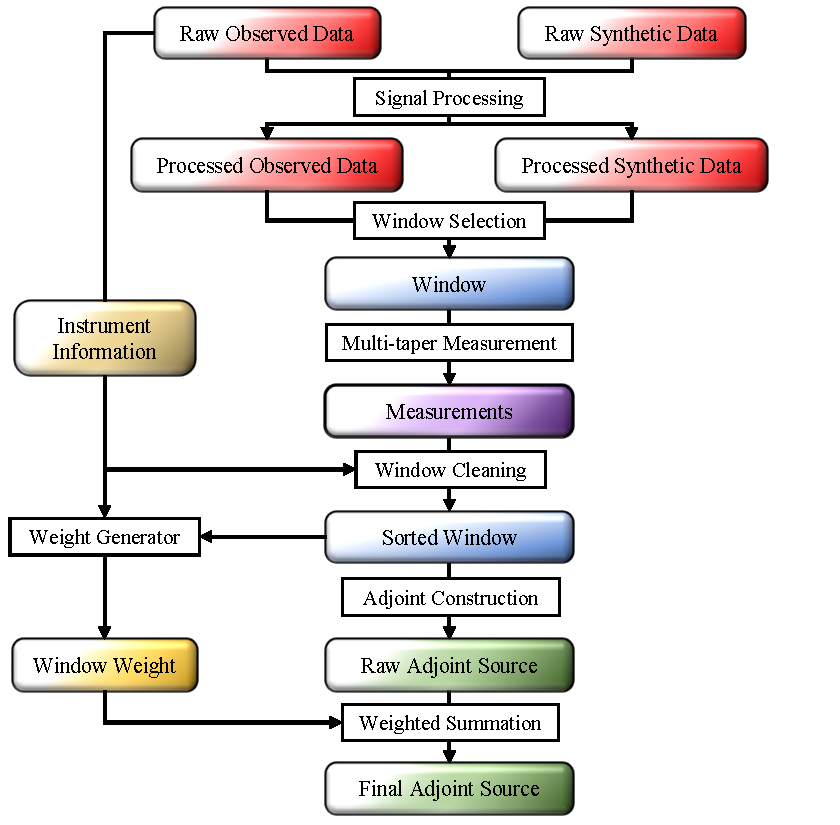
\includegraphics[width=0.8\textwidth]{ch-GLADM25/figures/Preprocess_workflow.pdf}
  \caption[Sub-workflow for pre-processing seismic data]
  {\small{Sub-workflow for pre-processing seismic data.}}
  \label{fig:preprocess_workflow}
\end{figure}

Python provides a great community environment and open-source support,
meaning that for most
of the lower level implementations we do not need write code, but
just find the right Python library.
For example,
Numpy and Scipy support common numerical and matrix operations.
For time series analysis,
Obspy is a Python-based seismic data analysis toolkit which provides
most signal processing operations, such as tapering, demeaning, detrending, filtering, and instrument response removal.
It is far more powerful than SAC,
providing rich APIs, including support for more versatile I/O methods, reading
various source formats (such as NDK, CMTSOLUTION, and QuakeML),
station formats (RESP, pole-zeros, StationXML),
and seismic data formats (e.g., SAC, MSEED, SEGY).
Also, ASDF uses HDF5 as the underlying data container,
and HDF5 already has numerous stable Python libraries, such as h5py,
to read and write HDF5 files in a serial or parallel manner.

Importantly, it is very easy to develop processing tools in a modular style in Python.
Integration of open-source Python packages,
such as Numpy, Scipy, and Obspy, takes much
less effort than writing in Fortran or C, thanks to Python's dynamic language features.
Python also provides and encourages use of very powerful software management systems,
such as pip and Anaconda,
and these tools come with version control capabilities.
All of these attriutes make it much simpler to develop tools in Python than in
Fortran, C, or C++.

There are some disadvantages to using Python.
A common complaint is lack of efficiency due to its dynamic nature.
Python will likely never match the performance of static compiled languages,
such as Fortran or C.
However,
frequently there are other factors that are more critical than speed,
such as fast development, easy deployment, and a user-friendly development environment.
For these reasons, Python has gained much popularity in data science and machine learning, where researchers rely extensively on Python to process big datasets.

In the following, we focus on software we developed
for the data processing workflow, which constitutes the preprocessing phase of the overall adjoint tomography workflow.

\subsection{Software}

\begin{figure}
  \centering
  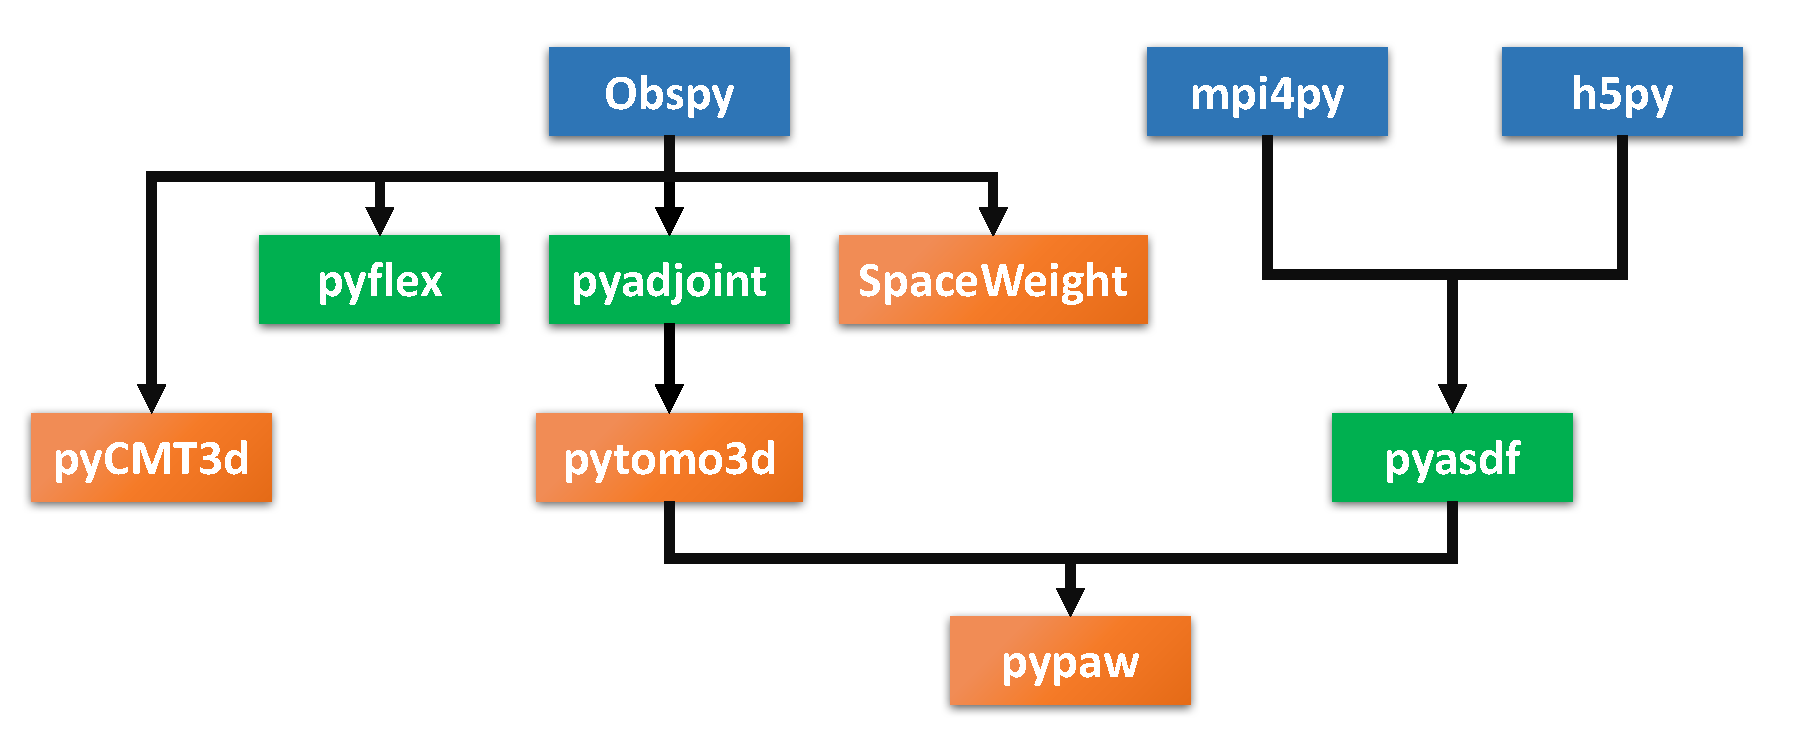
\includegraphics[width=0.98\textwidth]{ch-tools/figures/data_processing_software.pdf}
  \caption[software built for preprocessing seismic data]
  {\small{Software built for preprocessing seismic data. The position and arrows denote software dependencies. Colors denote the contribution level. Software with
  an orange box was mainly developed by me, while Greens boxes signify software I have contributed to, and blue boxes denote common open-source libraries (there are many open-source libraries we use; only major ones are listed.). All the software I developed is open source.}}
  \label{fig:preprocess_software}
\end{figure}


Fig.~\ref{fig:preprocess_software} shows the software tree we developed
for the seismic data processing workflow.
Obspy sits at the lowest level of the processing chain.
It provides APIs for operations on time series data. It is also used for
parsing QuakeML and StationXML files, rotating horizontal seismometer components, calculating arrival times and source and receiver azimuths, etc.
On top of Obspy we developed pycmt3d, pyflex, pyadjoint, and Spaceweight.
Pyflex, the Python version of the Fortran window selection tool FLEXWIN, is used to select time windows on a pair of observed
and synthetic traces.
A new feature we added to Pyflex is seismic
phase detection.
When selecting windows, Pyflex not only identifies seismic phases
based on arrival time calculations, it can also sort windows based on those phases.
This is very convenient when we only wish to select body waves during the window selection stage.
Pyadjoint, the Python port of measure\_adj, is used to make
various types of measurements and construct corresponding adjoint sources.
Spaceweight is a new software package to determine geographical source and stations weights,
which are attached to the adjoint sources and incorporated in the misfit function.
The package is mainly used for
balancing the uneven distribution of sources and stations (see Chapter~\ref{ch:weighting}).
Pycmt3d is a Python port of the Fortran package CMT3D used for seismic source inversions
In addition
to waveform misfits, an option for using envelope misfits has been built into the package,
and geographical weights based on spaceweight can also be assigned as part of the source inversion.

The Python package pytomo3d was created as a higher-level toolkit that integrates
pyflex, pyadjoint, spaceweight, and other utility functions.
Whereas pyflex and pyadjoint operate on the time series provide by obspy as
obspy.trace (one trace is one time series),
pytomo3d operates on a collection of time series provided by obspy as obspy.stream (one stream contains several traces, and in our case one stream
contains traces from the same station).
It is very natural for operations to be
applied at the stream level.
For example, rotating the two horizontal components 
from North and East to radial and transverse is one step in the signal processing
chain.
Basically, the stream options adds another level of abstraction.
Users only need to use APIs provided by pytomo3d,
rather than APIs from lower-level package.
If some lower-level packages become obsolete in the future, for example, pyflex might be
replaced by a more advanced window selection algorithm based on artificial intelligence,
users may not even be aware of that as long as we keep the APIs in pytomo3d unchanged. 
Those who do not use ASDF can utilize all the functionality provided by
pytomo3d and construct their own workflow, since pytom3d has no dependency on ASDF.

For the data container pyasdf branch, mpi4py and h5py sit at the lowest level. mpi4py is the Python version of MPI and handles messaging passing in a parallel environment.
H5py is a Python library for reading and writing hdf5 files.
Based on those libraries (there are more libraries we use, but here we mention the most important ones), we built
pyASDF, which provides the Python APIs for I/O based on ASDF.

At the top level, pypaw combines the data container and processing utility branches
by providing APIs for processing ASDF files during the data processing workflow.
It is used as part of the workflow management tools, which are discussed in the next section.

\section{Workflow Management}
\label{section:workflow_management}

The discussion thus far has focused on improvements of specific parts of the overall tomographic workflow,
such as the data format and time series analysis.
However, the volume of data and the magnitude of the numerical calculations
pose significant challenges for the overall workflow,
because hardware failures become inevitable, and human-induced errors are unavoidable.
The goal of using workflow management tools is to glue the entire inversion process together in a robust and stable fashion.
The main goal of workflow management tools is to use automation to
reduce human interference and errors.
In our global inversion,
we need to manage tens of thousands of ASDF files during each processing stage,
not to mention parameter and configuration files associated with
each data file. It is simply an impossible task to manage and monitor
manually.

By introducing workflow management tools,
we only need to setup the input and output
patterns for each processing stage, and data should
follow these patterns regardless of volume.
This has the additional benefit of reducing the overall time to solution for each iteration, since
each component can be connected without time gaps. 

Another benefit of workflow management is an increase in the robustness of the system.
With thousands of earthquakes and millions of seismic traces,
our inversion severely stresses compute nodes and the file system, and there are occasional hardware failures which cause jobs to fail.
Workflow management tools should have the capability to
detect such failures and recover from them.
Only jobs which pass validation may be labeled as completed and continue to the next stage of processing.

After exploring several existing workflow management tools,
we selected the Ensemble ToolKit (EnTK)~\cite{EnTK2017} developed by the RADICAL
group from Rutgers University.
In this environment,
the simpy (Seismic Inversion Management PYthon) toolkit was developed using RADICAL-SAGA, pypaw, and sqlite3.
RADICAL-SAGA works as the 
job management component responsible for communicating with the queue of the HPC system,
pypaw provides user-defined processing components,
and sqlite3 is used as a bookkeeping database to keep track of job statuses.

Before the start of processing,
simpy validates all input and parameter files and stores them
into the sqlite3 database.
All initial jobs are labeled as `new'.
As the workflow starts, simpy submits jobs using 
RADICAL-SAGA as the job manager engine to communicate with the HPC system.
As soon as a job finishes, simpy receives notifications from
RADICAL-SAGA and launches a job validation process.
Once job passes validation,
it labels the job as `done' in the database.
If the job fails, simpy labels
the job status according to the error type and re-submit failed jobs in batch mode.
By utilizing existing tools like RADICAL-SAGA, we only need to focus on the user logic rather
than job management, thereby offloading work to those libraries.
RADICAL-SAGA has the capability to communicate with many job submission systems,
so it can potentially be deployed on many other supercomputer systems without any
code changes (although some configuration changes may still be required).

As a most recent development, we integrated EnTK
into our forward and adjoint simulation workflows. Our ultimate
goad is to develop a workflow tool that works across platforms and integrates one entire tomographic iteration, including forward simulations, data processing, adjoin simulations, and post-processing.

\chapter{Balancing Unevenly Distributed Data in Seismic Tomography: {A} Global Adjoint Tomography Example\label{ch:weighting}}

\textbf{Note}\\
This chapter has been submitted as a paper entitled ``Balancing Unevenly Distributed Data in Seismic Tomography: {A} Global Adjoint Tomography Example'' by Ruan, Y., Lei, W., Modrak, R., \"{O}rsvuran, R., Bozda\u{g}, E., and Tromp, J.\ to the \textit{Geophysical Journal International}.


\section*{Summary}
The uneven distribution of earthquakes and stations in seismic tomography leads to slower convergence of nonlinear inversions and spatial bias in inversion results.
Including dense regional arrays, such as USArray or Hi-Net, in global tomography causes severe convergence and spatial bias problems, against which conventional preconditioning  schemes are ineffective.
To save computational cost and reduce model bias, we propose a new strategy based on a geographical weighting of sources and receivers.
We validate this strategy in
a 2D global waveform inversion test and show that the new weighting scheme leads to a nearly two-fold reduction in model error and much faster convergence relative to a conventionally-preconditioned inversion.
We implement this geographical weighting strategy for global adjoint tomography.

%%%%%------------------------------------------
%
%   1, 
%
%%%%---------------------------------------------
\section{Introduction}
%Highlight points:

The deployment of new global and regional seismographic stations has made  more data available for seismic tomography than ever before.
The spatial distribution of these stations remains highly lopsided, however, with limited Ocean Bottom Seismometers (OBSs) or ocean island stations,
%it's ocean island basalt, so I think it's also ocean island station
and fewer stations in the southern hemisphere than in the northern hemisphere. 
This uneven station coverage, combined with the uneven distribution of earthquakes dictated by plate tectonics, poses major challenges for the inverse problem.   In global adjoint tomography in particular, the large number of paths from subduction zones, such as Fiji-Tonga, to dense arrays,  such as USArray,  causes highly oscillatory behavior in model updates, hindering convergence~\cite{bozdaug2016global}. 

Since the first global tomographic study by~\cite{Dziewonski77}, uneven data coverage has been an issue of concern. 
The problem with a cluster of earthquakes or a dense receiver array is that data residuals are correlated, and large portions of data are in some sense redundant.  %This redundant information is then amplified in the inversion by force of numbers.    
The correlation of data residuals is reflected in the data covariance matrix: 
its diagonal terms are the measurement error of each datum, and off-diagonal 
terms indicate coherence between the errors of two corresponding data.
Ideally, data errors are independent, in which case only diagonal terms
need to be considered, and off-diagonal terms can be safely ignored.  When measurements are strongly 
correlated, the off-diagonal terms become relevant.  

Although uneven data coverage is a well-known issue in seismic tomography,
there is limited literature on how it should be properly dealt with.
In an important global seismic tomography study by~\cite{Li1996}, uneven data coverage was addressed by weighting the diagonal terms of the data covariance matrix according to how significant 
their errors are correlated with the errors of the other data.
The weighting function 
in this study ($\omega = \omega_e\, \omega_n  \,\omega_r$) consists of data errors 
($\omega_e$ --- the rms amplitude of a wave packet), data redundancy within a wave packet ($\omega_n$ --- the inverse of the square root of number of data), and data redundancy 
amongst wave packets sampling similar ray paths 
($\omega_r$ --- a geometrical relationship between a given source-receiver 
pair to all other pairs).
The final term addresses data covariance through a path weighting strategy and has been employed in a few subsequent global tomography studies \cite{SchaefferLebedev13}.  
In this paper, we adopt a similar but more general approach to handle unevenly distributed measurements.  

The effects of uneven data coverage depend to some extent on the model parameterization and 
regularization in a given inversion.  \cite{Boschi1999} examined the effects of uneven data 
coverage with differently parameterized and regularized inversions. They parameterized their global 
model in terms of both blocks and spherical harmonics.
Sparse data coverage in the southern hemisphere
produced fictitious model features, especially in the spherical harmonic model.
Applying stronger 
regularization or damping, however, more or less resolved the issue.
In other words, to resolve bias in inversions caused by uneven data coverage, we need to sacrifice resolution in well-covered regions through stronger damping.
Their experiments justify to some extend the use of 
strong damping in some global inversions~\cite{Masters1996,Antolik2003}.      

Besides geographical weighting, 
other strategies have been developed in different contexts~\cite{grand1994, s362ani, ritsema2011s40rts, Moulik2016}.
For instance, the use of weights based on analyst-assessed data quality or weights for jointly inverting disparate data types (e.g., seismic and gravity measurements). 
These weighting choices are sometimes ad hoc and vary from one practitioner to another.
In this study, we focus on weighting with the goal of balancing uneven data coverage, without drawing many connections with other types of weighting.
Since full-waveform adjoint tomography is computationally expensive, it is important to address slow convergence due to unevenly distributed data.  
Here, we focus on a robust weighting strategy that can be applied to 
unevenly distributed earthquakes and stations to balance their contributions.

\section{Weighting strategy}
\label{sec:dataproc}

\subsection{Measurements and Misfit Function}

Seismic waves sample different parts of Earth's interior at different dominant frequencies, so it is natural to 
categorize seismic signals in terms of their type and band.
In global adjoint tomography~\cite{bozdaug2016global, Lei2018}, we currently consider three period 
bands: 17--40~s,  40--100~s, and 90--250~s. 
Typically, we select body waves in the 17--40~s band,
body waves in the 40--100~s band,
surface waves in the 40--100~s band,
and surface waves in the 90--250~s band.
Within each band, we consider three-component 
seismograms rotated into vertical, radial, and transverse directions 
of motion, so in total there are twelve data categories, as summarized in 
Table~\ref{table:categories}. 

\begin{table}
\caption[Measurement categories in global adjoint tomography]
{\small{Measurement categories in global adjoint tomography~\cite{bozdaug2016global, Lei2018}.
    Seismic waves are categorized in terms of complementary 
    period bands on three components of motion.}}
\begin{tabular}{|c|c|c|c|}
\hline

~         &  Vertical (Z) & Radial (R) &  Transverse (T) \\
\hline
17--40~s           &   P-SV body waves                        & P-SV body waves                       & SH body waves   \\
40--100~s         &   P-SV body waves                        & P-SV body waves                       & SH body waves \\
40--100~s         &   Rayleigh waves                           & Rayleigh waves                           & Love waves \\
90--250~s         &   Rayleigh waves                           & Rayleigh waves                           & Love waves \\
\hline
\end{tabular}\\
\label{table:categories}
\end{table}

Considering all these data categories, along with all the sources and receivers available for an inversion, we define an overall data misfit
\begin{equation}
\label{eq:misfit}
\Phi = \sum_{s=1}^{S} \omega_s \sum_{c=1}^{C} \omega_{c} \sum_{r=1}^{R_{sc}} \omega_{scr} \sum_{w=1}^{N_{scr}} \omega_{scrw}\, \chi_{scrw}
\quad .
\end{equation}
Here, $s = 1, ... , S$ denotes a given source and~$S$ the total number of sources.  Likewise, $c = 1, ..., C$ denotes a given category and~$C$  the total number of categories (in our case, the twelve categories summarized in Table~\ref{table:categories}).
$R_{sc}$ denotes the number of receivers for a given source~$s$ and category~$c$. Finally, $N_{scr}$ denotes the number of measurement windows for a given source~$s$, category~$c$, and receiver~$r$.

The misfit for a given source~$s$,
category~$c$, receiver~$r$, and measurement window~$w$ is
\begin{equation}
\label{eq:misfit_def}
\chi_{scrw} = \left(\frac{\Delta d_{scrw}}{\sigma_{scrw}}\right)^2
\quad ,
\end{equation}
where~$\Delta d_{scrw}$ denotes a measurement with associated uncertainties~$\sigma_{scrw}$.
When the model fits the data to within one standard deviation, we expect that
\begin{align}
\chi_{scrw} \sim 1
\quad .
\end{align}
In the following sections we discuss various options for the assignment of the 
source, category, receiver, and window weights~$\omega_s$,
$\omega_{c}$, $\omega_{scr}$, and~$ \omega_{scrw}$, respectively.
%===
%
%===
\subsection{Category-weighting strategy}
\label{sec:simple}

We start by considering an ideal case where each datum in a certain category is independent and the 
associated errors are not correlated.  (In reality, the measurement error
of a datum is difficult to estimate, not to mention the correlation of the errors.) 
The standard deviation~$\sigma_{scrw}$ in eqn.~(\ref{eq:misfit_def}) is often 
set as an {\it a priori} constant in the practice of inversion.
Under such conditions, a common weighting strategy is to assign a constant 
weight to all windows, receivers, and sources, i.e.,
\begin{align}
\omega_{s} & =  1 \quad, \\
\omega_{scr} & = 1 \quad, \\
\omega_{scrw} & = 1 \quad.
\end{align}

We seek to define a misfit function~$\Phi$ such that when the model fits the data 
to within one standard deviation, $\Phi\sim 1$\,. The data in each category  
should contribute equally to the overall misfit,  which implies that we should choose a category weight
\begin{align}
\label{eq:simple_w}
\omega_{c} = \frac{1}{C}\,\frac{1}{N_c}
\quad,
\end{align}
where~$N_c$ is the number of measurements in category~$c$, that is
\begin{align}
\label{eq:Nc}
N_c=\sum_{s=1}^{S}\sum_{r=1}^{R_{sc}} \,N_{scr}
\quad .
\end{align}
Note that the category weight in eqn.~(\ref{eq:simple_w}) is independent of source~$s$.
Now we see that when the model fits the data to within one standard deviation, 
i.e., $\chi_{scrw} \sim 1$, then
\begin{align}
\Phi & \sim \sum_{s=1}^{S} \omega_s \sum_{c=1}^{C} \omega_{c} \sum_{r=1}^{R_{sc}} \omega_{scr} \sum_{w=1}^{N_{scr}} \omega_{scrw} \\
& = \sum_{s=1}^{S} \sum_{c=1}^{C} \omega_{c} \sum_{r=1}^{R_{sc}} N_{scr} \\
& = \sum_{c=1}^{C} \frac{1}{C}\,\frac{1}{N_c} \sum_{s=1}^{S} \sum_{r=1}^{R_{sc}} N_{scr} \\
& = \sum_{c=1}^{C} \frac{1}{C} \\
& = 1
\quad ,
\end{align}
as desired.

Let us next analyze the contribution of each datum to the misfit function at various levels.
At the receiver level, we consider
\begin{equation}
\label{eq:reclev}
\chi_{scr} = \sum_{w=1}^{N_{scr}} \omega_{scrw} \, \chi_{scrw}
\quad .
\end{equation}
When we assign a weight of one to all windows,
i.e., $\omega_{scrw}=1$, thus putting them on the same footing,
and when the model fits the data to within one standard deviation, i.e., $\chi_{scrw} \sim 1$, we see that
\begin{equation}
\label{eq:simple_scr}
\chi_{scr} \sim N_{scr}
\quad .
\end{equation}
Next, we consider the misfit for a given source~$s$ and category~$c$, namely
\begin{equation}
\label{eq:catlev}
\chi_{sc} = \sum_{r=1}^{R_{sc}} \omega_{scr} \sum_{w=1}^{N_{scr}} \omega_{scrw}\, \chi_{scrw} = \sum_{r=1}^{R_{sc}} \omega_{scr}\, \chi_{scr}
\quad .
\end{equation}
When the model fits the data to within one standard deviation, we find that
\begin{equation}
\label{eq:simple_cs}
\chi_{sc} \sim \sum_{r=1}^{R_{sc}} N_{scr} = N_{sc} 
\quad ,
\end{equation}
where~$N_{sc}$ denotes the number of measurements for a given source~$s$ in category~$c$.
Note that we have used the fact that~$\omega_{csr}=1$, meaning all receivers are weighted equally. 

Since category weighting is independent of source weighting,
we can change the order of summation.
The misfit in a given category~$c$ is given by
\begin{equation}
\chi_{c} = \sum_{s=1}^{S} \omega_s\,\chi_{sc}
\quad .
\end{equation}
Since~$\omega_{s} = 1$,
we see that when the model fits the data to within one standard deviation
\begin{equation}
\label{eq:simple_chi_c}
\chi_c \sim \sum_{s=1}^{S}N_{sc}=N_c
\quad ,
\end{equation}
as expected.

Finally, the total misfit function is
\begin{equation}
\Phi = \sum_{c=1}^{C} \omega_{c} \,\chi_{c}
\quad ,
\end{equation}
and thus we see that when the model fits the data to within one standard deviation
\begin{equation}
\Phi \sim \sum_{c=1}^{C} \frac{1}{C}\, \frac{1}{N_c} \,N_c = 1
\quad .
\end{equation}
as required. This weighting scheme is widely used in a variety 
of inversions~\cite{zhu2015seismic, bozdaug2016global}.
The behavior of the misfit function at the various levels demonstrated above will guide 
the design of source and receiver weights in the next section.
%===

\subsection{Geographical-weighting strategy}
\label{sec:geographical_weights}

In the previous section we treated each measurement datum in a given category 
equally, which means each datum was weighted only by the total number of measurements 
in its category, regardless of possible correlations between data. Solving the 
inverse problem based on this ``all data are equal'' strategy can fail sometimes, 
because the uneven spatial distribution of sources 
and receivers on Earth's surface is found to negatively affect convergence rate. 
In particular, if data from dense regional arrays such as USArray are included,  progress 
of the inversion can be extremely slow.  
In this section, we add additional weights associated with the geographical 
distribution of sources and receivers, with the goal of down-weighting 
densely sampled regions, so that we obtain more uniform spatial sampling
and minimize the dominant effects of dense regional arrays. 
  
%===
\subsubsection{Geographical Weighting}
\label{sec:geographical}

For closely located sources or dense receiver arrays, measurement errors 
are correlated for a variety of reasons~\cite{Li1996}, and the degree of correlation 
is associated with geographical distance.
With these correlations in mind, we seek to define a source and receiver weighting scheme 
that results in more uniform spatial sampling.  In such a scheme, areas with dense sampling, 
like Japan or North America, should be down-weighted relative to areas which are sparsely 
sampled, such as the Southern Ocean.  %In such way that in the inversion the redundant paths from an event cluster to a dense array, for instance, Fiji-Tonga earthquakes to USArray stations, would not dominate the model update and allow the important features in the regions with relatively sparse coverages to emerge. 

To determine weights for each source and receiver, one option is to construct a Voronoi tessellation~\cite{Du1999} of the sources or receivers, 
and then weight each source or receiver by the area of its corresponding cell.
Unfortunately, this approach can lead to instabilities, because stations at the edge of a dense array can be weighted orders of magnitude more than stations slightly away from the edge. 

A robust alternative approach is as follows.  Given a set of~$N$ receivers, 
calculate the epicentral distance~$\Delta_{ij}$ for each receiver pair. 
The weight~$\omega_i$\, assigned to each receiver~$i$ is calculated via
\begin{equation}
\omega_{i}^{-1} = \sum_{j=1}^N \exp \left[\mbox{}- \left(\frac{\Delta_{ij}}{\Delta_0}\right)^2\right]
\quad ,
\label{eq:spatial_weights}
\end{equation}
where~$\Delta_{0}$ is a reference distance parameter.
We note that if a station has few nearby stations, it is assigned a larger weight than if it has many nearby 
stations.
For large values of~$\Delta_0$ the scheme reduces to the category weighting in Section~\ref{sec:simple}.

We also note that an equivalent weighting scheme for sources can be obtained by substituting source pairs for receiver pairs in the above expression.
In Section~\ref{sec:norm} we discuss how  weights determined by eqn.~(\ref{eq:spatial_weights}) are normalized to obtain weights~$\omega_{c}$ for each event and~$\omega_{csr}$ for each receiver associated with a certain event.

Interestingly, eqn.~(\ref{eq:spatial_weights}) is just a discretized version of the 
``regularization by convolution" method used in many parameter estimation and optimal 
design studies~\cite{Modrak2016}. Rather than using convolution to smooth the gradient 
of an objective function, however, we are using it to ``smooth'' the uneven discrete receiver 
distribution. 

\subsubsection{Choice of reference parameter}
\label{sec:ref-par}

The distribution of weights calculated from eqn.~(\ref{eq:spatial_weights}) depends strongly on the reference distance~$\Delta_0$.  This parameter needs to be carefully chosen so that the ratio of maximum to minimum  weights is not unreasonably small or large. 
In the example in Figure~\ref{fig:weight_condnum}, we chose~$\Delta_0$ so that the ratio is about one third of the largest possible ratio for all choices of~$\Delta_0$.  In other words, we chose the reference length parameter to be about one third of the most aggressive value.

\begin{figure}
    \centering 
 	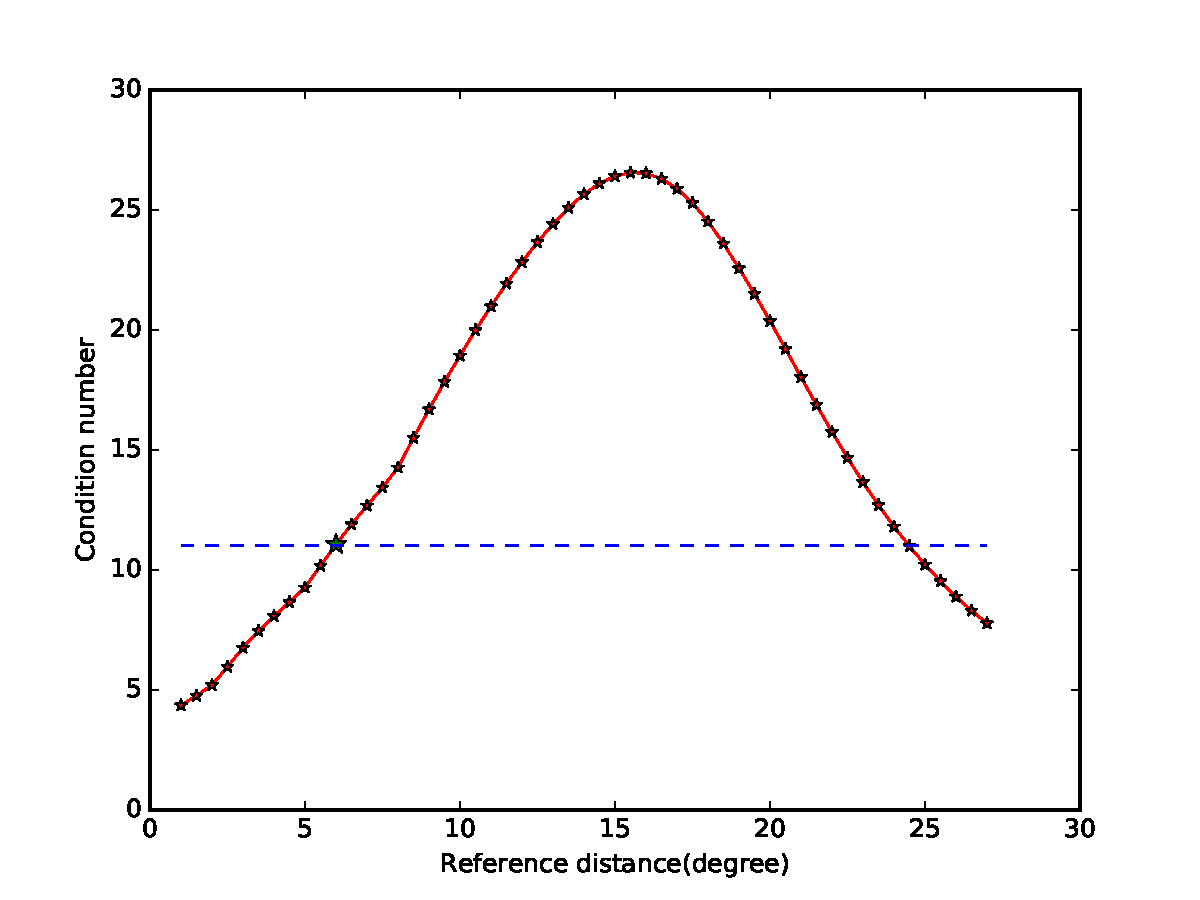
\includegraphics[width=.95\textwidth]{ch-weighting/figures/source_weight_cond_num.pdf}
  \caption[Condition number curve of the diagonal weighting matrix]
  {\small{Condition number of the diagonal weighting matrix defined by eqn.~(\ref{eq:spatial_weights})
as a function of the reference distance~$\Delta_0$\,.
The chosen value, indicated by the green star, is about one third of the largest possible value.
Since evaluation of eqn.~(\ref{eq:spatial_weights}) for different reference distances adds negligible computational expense, it is possible (and recommended) to repeat this type of analysis for each iteration.
}}
\label{fig:weight_condnum}
\end{figure}

Based on this choice, Figures~\ref{fig:receiver_weights} and \ref{fig:source_weights} illustrate the
distribution of weights in a recent global adjoint tomography study~\cite{Lei2018}. In Figure~\ref{fig:receiver_weights},
USArray and European stations weights are brought down to about one-tenth of ocean island station weights. The source weighting is similar, with the contribution of individual Fiji Tonga events brought down to about one-tenth the contribution of intraplate events in Asia. This ratio between the minimum and maximum weights can be adjusted through the reference distance parameter, as informed by practical experience in a given inversion.

\begin{figure}
 \centering 
   	\begin{minipage}[t]{.9\columnwidth}
  	\centering 
 	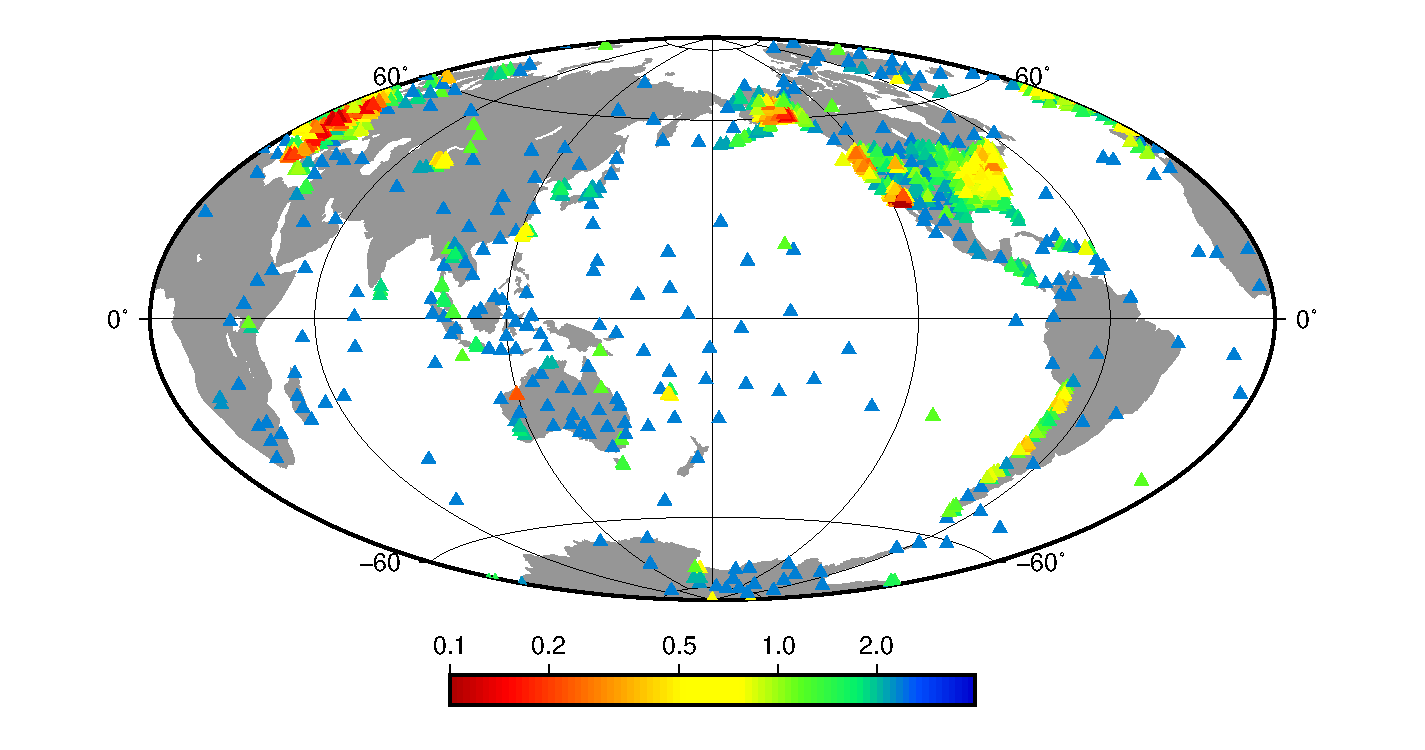
\includegraphics[width=.95\textwidth]{ch-weighting/figures/receiver-weights-40-100-Z.pdf}
	\end{minipage}
  \caption[Example of receiver weights]
  {\small{Example of receiver weights for an event C201604131355A at 40--100~s period band and vertical component determined based upon eqn.~(\ref{eq:spatial_weights}),
and normalized according to eqn.~(\ref{eq:recnorm}). The weights are in logarithmic scale.
Note the difference between USArray stations 
and ocean island stations. 
}}
\label{fig:receiver_weights}
\end{figure}

\begin{figure}
 \centering 
   	\begin{minipage}[t]{.9\columnwidth}
  	\centering 
	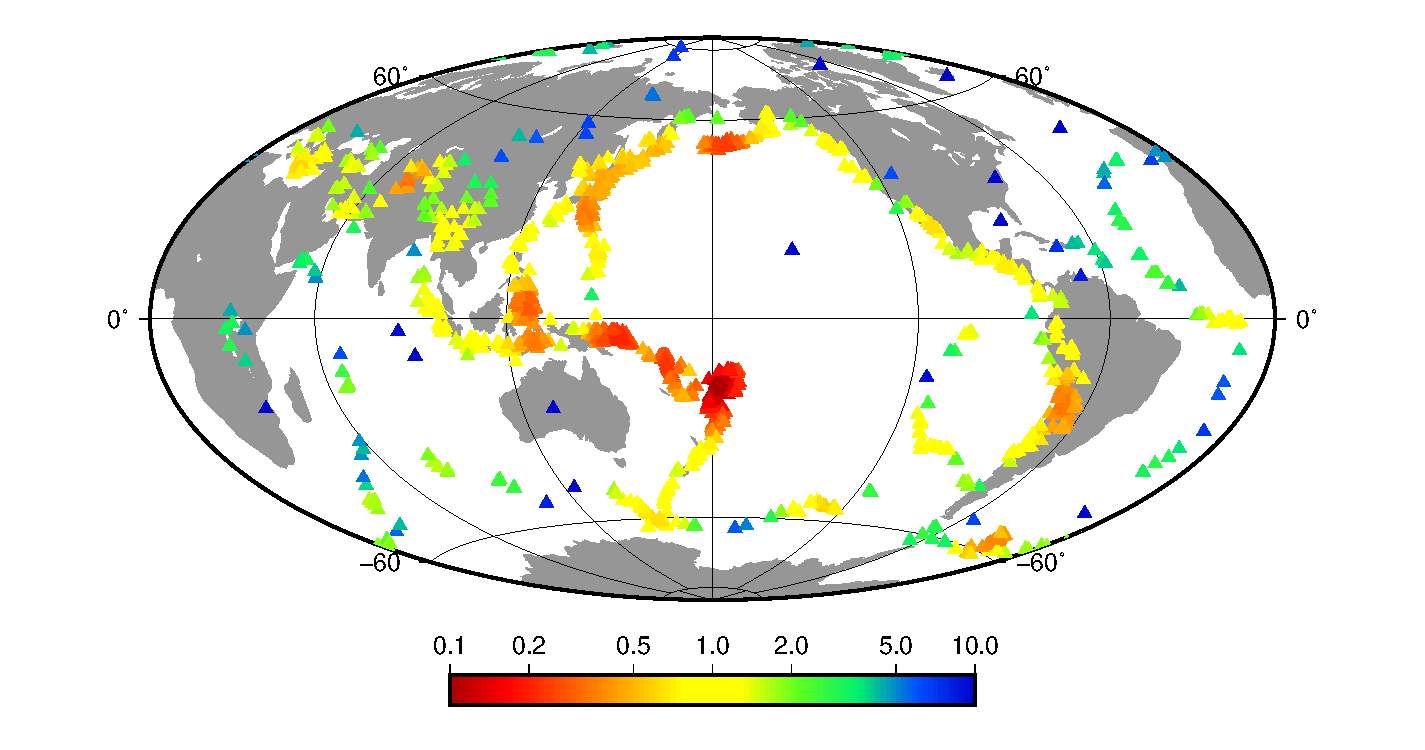
\includegraphics[width=.95\textwidth]{ch-weighting/figures/source-weights.pdf}
	\end{minipage}
  \caption[Example of source weights]
  {\small{Example of source weights determined based upon eqn.~(\ref{eq:spatial_weights}),
and normalized according to eqn.~(\ref{eqn:src_norm}).
Note the difference between dense subduction zone
earthquakes and sparse transform fault earthquakes.  
}}
\label{fig:source_weights}
\end{figure}

%===
\subsubsection{Weighting Normalization}
\label{sec:norm}

In this section our goal is to introduce geographical source and receiver weighting without changing the event- and category-level behavior of the misfit function discussed in Section~\ref{sec:simple}.  

In geometrical ray-based tomography, specific phases are identified and windowed. These phases usually correspond to distinct paths that provide constraints 
on different parts of Earth's interior, and some phases may be assigned more weight than others 
depending on the aims of the researcher.
In waveform inversion, any part of the wave train can 
be selected and phase identification is no longer required. We thus assign a uniform weight to all windows in a seismogram,
\begin{equation}
\label{eq:I_omega_scrw}
\omega_{scrw} = 1
\quad ,
\end{equation}
such that, according to eqn.~(\ref{eq:simple_scr}), $\chi_{scr}\sim N_{scr}$.
The normalization of the geographical source weights from eqn.~(\ref{eq:spatial_weights}) 
is then determined in a straightforward manner by
\begin{align}
\label{eqn:src_norm}
\sum_{s=1}^{S} \omega_{s} = S
\quad .
\end{align}

Because the number of receivers that happen to be online varies from one source to another, including receiver weights in an inversion is not as straightforward.
To guide the normalization of receiver weights, we adopt the same type of analysis performed in connection with category-weighting and eqn.~(\ref{eq:catlev}).

If the model fits the data to 
within one standard deviation, the misfit in a certain source and category ~$\chi_{sc}$ approaches~$N_{sc}$, and the receiver-level misfit ~$\chi_{scr}$ approaches~$N_{scr}$ 
(eqns.~\ref{eq:simple_scr}--\ref{eq:simple_cs}).
These properties of the misfit imply a normalization requirement for the receiver weights~$\omega_{scr}$, 
determined by eqn.~(\ref{eq:spatial_weights}) for a given category~$c$ and source~$s$:
\begin{align}
\label{eq:recnorm}
\sum_{r=1}^{R_{sc}} \omega_{scr} \, N_{scr} = N_{sc}
\quad .
\end{align}
When~$\omega_{scr} = 1$, as in the simple weighting strategy, this normalization 
condition is naturally satisfied because
\begin{equation}
\sum_{r=1}^{R_{sc}} N_{scr} = N_{sc}
\quad .
\end{equation}
After we determine the source and receiver weights, what is left is to examine the category weights~$\omega_c$\,.
For the misfit function given by eqn.~(\ref{eq:misfit}), we want the contributions from each category to be balanced, 
and this implies that
\begin{align}
\omega_{c} \sum_{s=1}^{S}\, \omega_s \sum_{r=1}^{R_{sc}} \omega_{scr}\,N_{scr}
=
\omega_{c} \sum_{s=1}^{S} \omega_s\, N_{sc}
= \frac{1}{C} 
\quad ,
\end{align}
and thus
\begin{align}
\omega_{c} = \frac{1}{C}\,\frac{1}{ \sum_{s=1}^{S} \omega_s\, N_{sc}}
\quad .
\end{align}
Note that when~$\omega_s=1$, the weighting reduce to the category-weighting strategy, namely
\begin{align}
\omega_{c} = \frac{1}{C}\,\frac{1}{ N_{c}}
\quad .
\end{align}

From the normalization of geographical weights described above, we see that when the model 
fits the data to within one standard deviation, the source-level misfit ~$\chi_{sc}$ approaches~$N_{sc}$
and category-level misfit~$\chi_{c}$ approaches~$N_{c}$.

In theory, data correlation changes the degrees of freedom in the data space 
of an inversion.
Loosely speaking,
the above normalization can be thought of as changing  the degrees of freedom of the dataset for a given category~$c$ and source~$s$, as well as the degrees of freedom of the dataset in a given category~$c$.
Geographical weighting can be viewed as an approximation of the complete 
data covariance matrix. 
%%%%%------------------------------------------
%
%   2, 
%
%%%%---------------------------------------------
\section{Numerical Validation: 2D Global Adjoint Tomography}

\begin{figure}
    \centering
    \begin{minipage}[t]{.9\columnwidth}
    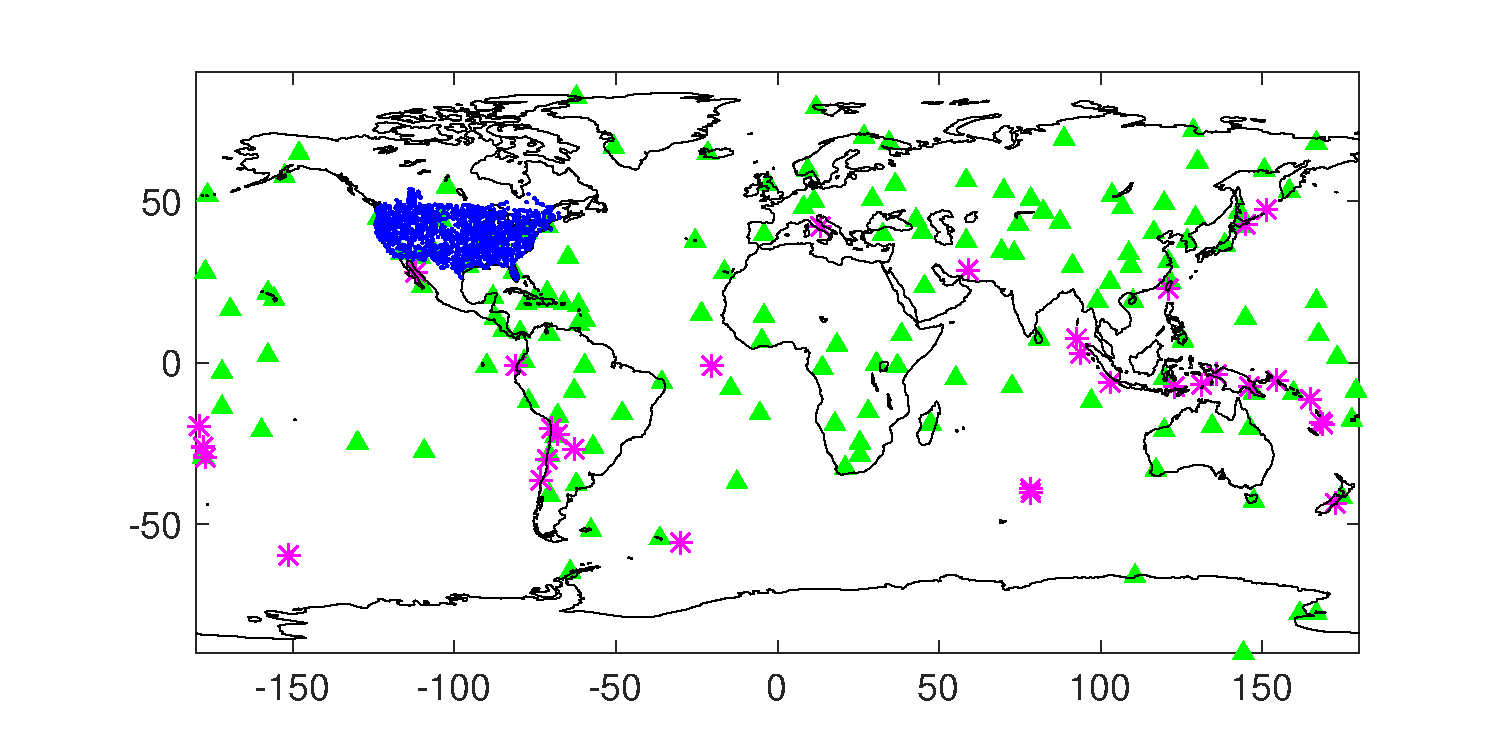
\includegraphics[width=.95\textwidth]{ch-weighting/figures/network.pdf}  %\\
    \end{minipage}
  \caption[source-receiver geometry used in synthetic inversions]
  {\small{Source-receiver geometry used in synthetic inversions.  
GSN stations are labeled by green triangles, USArray stations by blue triangles, and sources 
by magenta asterisks.
}}
\label{fig:test-src-sta}
\end{figure}

To test the geographical weighting strategy, 
we performed 2D inversions with a global test problem.  In these experiments, we used both GSN stations, which are sparsely distributed 
at the global scale, and USArray stations, which densely cover the North American continent, as shown in Figure~\ref{fig:test-src-sta}.
For the target model, we employed the acoustic test case  shown in Figure~\ref{fig:test-model}.  We generated synthetic data for this model using periodic boundary 
conditions at the edges to approximate a spherical Earth.  Finally, we inverted these data  with the workflow described by~\cite{Modrak2018}.  

\begin{figure}
    \centering
    \begin{minipage}[t]{.9\columnwidth}
    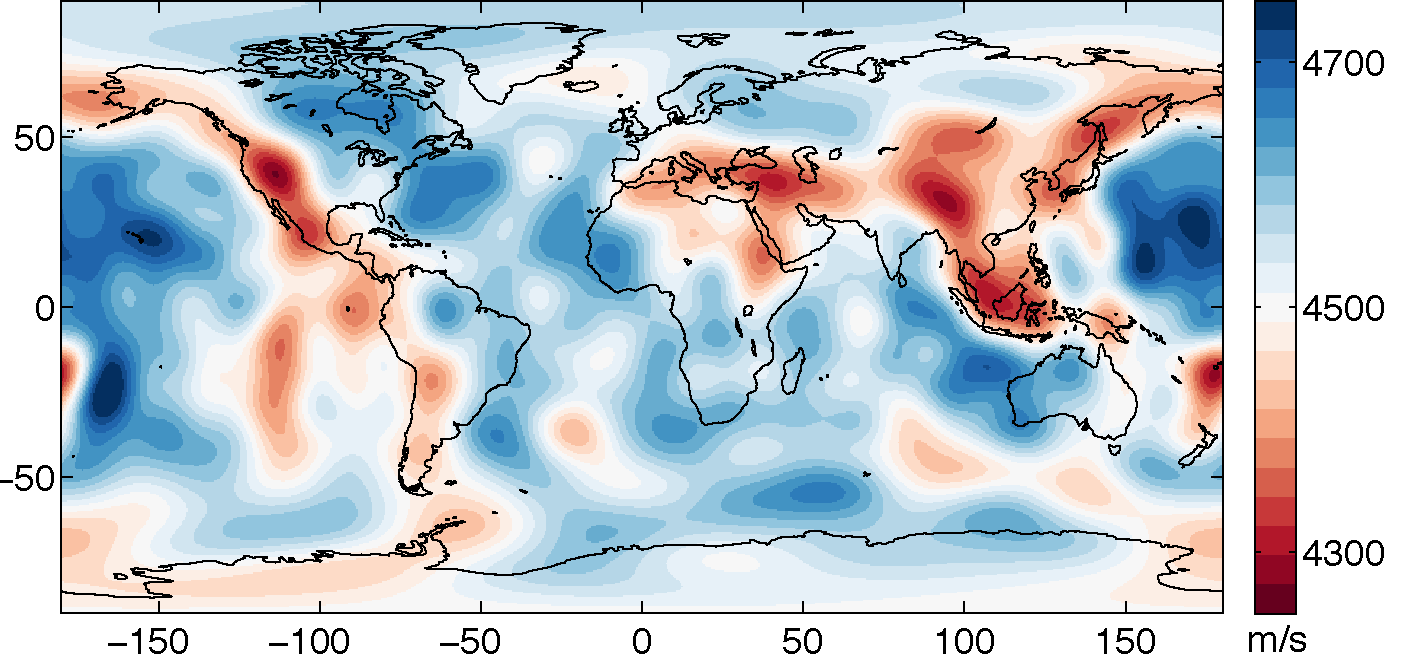
\includegraphics[width=.9\textwidth]{ch-weighting/figures/2Dmodel.pdf}  %\\
    \end{minipage}
  \caption[Target model used in the synthetic inversions for testing weighting strategies]{\small{Target model used in the synthetic inversions. Wavespeeds are determined by the 40~s Rayleigh wave phase speed model of~\cite{Trampert2003}.
}}
\label{fig:test-model}
\end{figure}
 
Starting from a homogeneous model, we tracked the reduction in model error as a function of the number of wavefield simulations in three separate inversions.
In the first inversion, we employed model-space diagonal preconditioning, using the best-performing preconditioner of all the variants tested by~\cite{Modrak2016}.
In the second inversion, we employed the category-weighting 
strategy discussed in Section~(\ref{sec:simple}).  
 In the third inversion, we used the geographical-weighting strategy described in Section~\ref{sec:geographical_weights}. The performance of the three methods is shown in Figure~\ref{fig:convergence}. 

\begin{figure}
    \centering
    \begin{minipage}[t]{.9\columnwidth}
    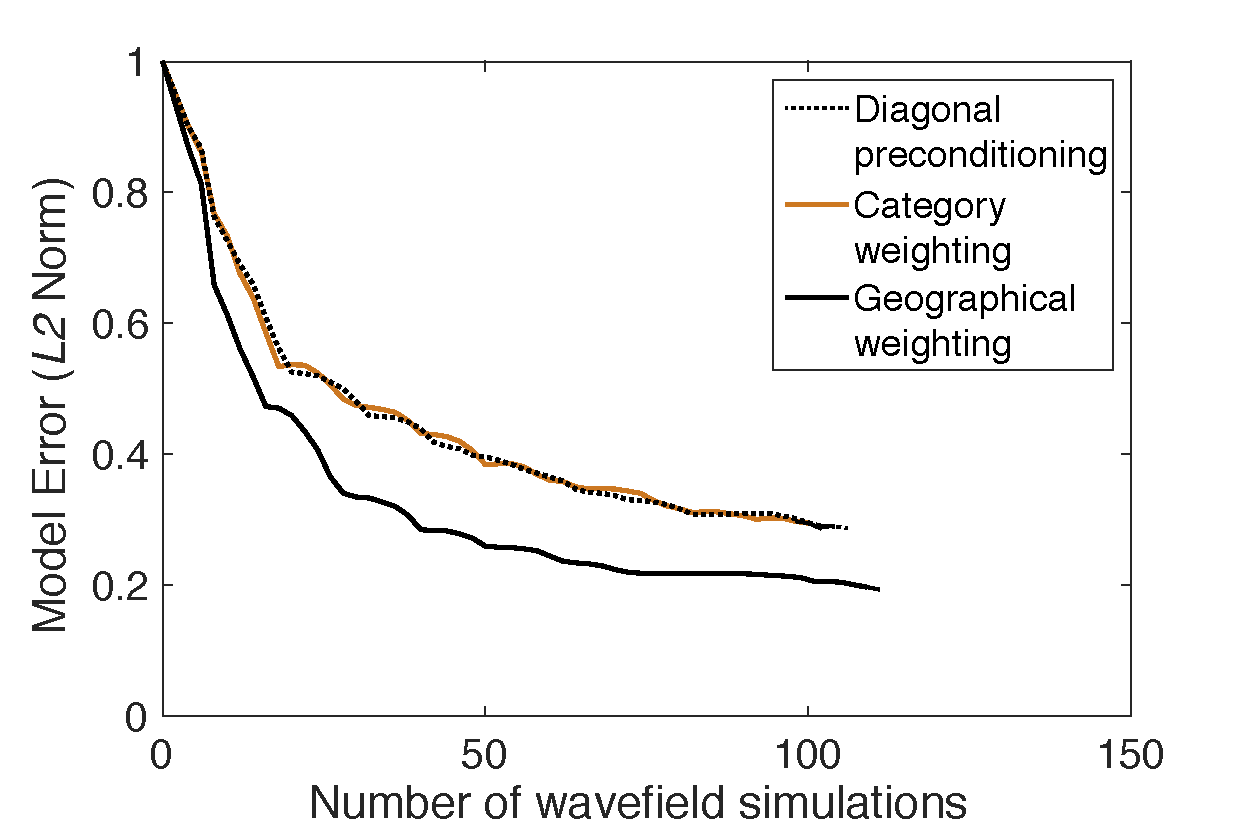
\includegraphics[width=.8\textwidth]{ch-weighting/figures/convergence_tests.pdf}  %\\
    \end{minipage}
  \caption[Convergence Test for different weighting strategies]
  {\small{With the category weighting defined in Section~\ref{sec:simple}, convergence is extremely slow.  
With the geographical weighting discussed in Section~\ref{sec:geographical_weights}, convergence is much faster.  
Diagonal model-space preconditioning, it turns out, is not an effective alternative to weighting when dealing with extremely lopsided source-receivers distributions.
}}
\label{fig:convergence}
\end{figure}

Compared with category weighting, preconditioning fails to provide an effective improvement, while the geographical-weighting 
strategy provides a much faster convergence rate. Considering the high cost of large-scale inverse problems 
like global adjoint tomography, where one iteration can require  millions of core hours, 
the saving could be significant. In addition to the performance improvement, the geographically-weighted inversion 
 demonstrates larger model error reduction than the other  approaches. 
%%%%%------------------------------------------
%
%   3, 
%
%%%%-------------------------------------------
\section{Application to 3D Global Adjoint Tomography: Misfit Statistics}

\begin{figure}
\centering
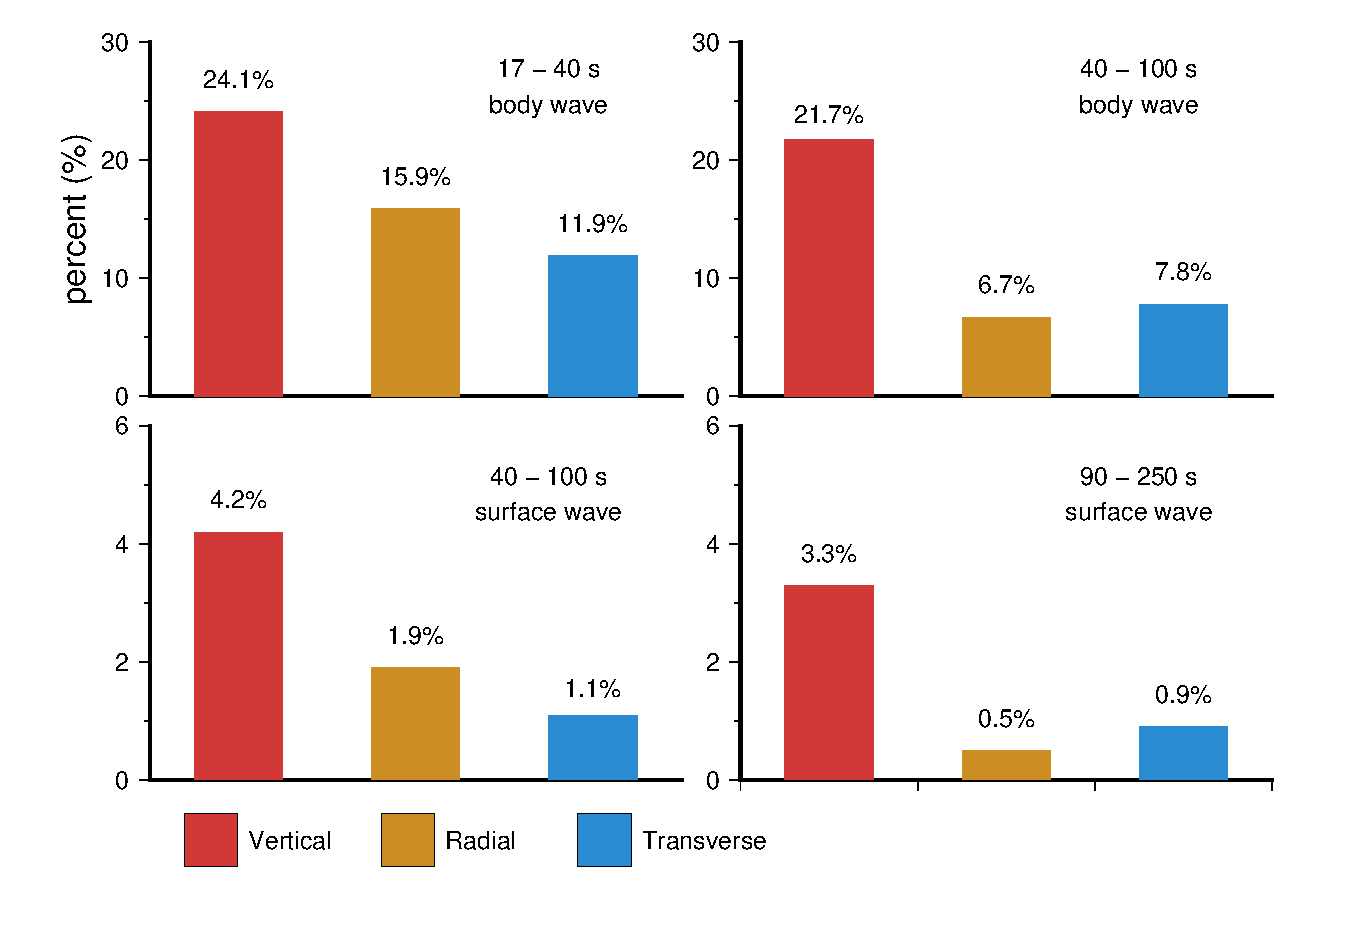
\includegraphics[width=0.8\textwidth]{ch-weighting/figures/category_wincount_contribution.pdf}
  \caption[Percentage of data in the twelve categories]
  {\small{Percentage of data (window count) in each of the twelve categories (see Table~\ref{table:categories}).
Period band and wave type are  labeled in the upper right corner of each panel.
Note the dramatic differences between  
body-wave (top) and surface-wave data (bottom). 
The large variations in data count from category to category illustrate the 
need for balancing.
}}
\label{fig:wcounts_contribution}
\end{figure}

After testing the geographical-weighting strategy through synthetic experiments,
we deployed it in our ongoing
global adjoint tomography study~\cite{Lei2018} with the goal of obtaining faster convergence and a 
better model. In this section we illustrate various aspects of the above category- and geographical-weighting
strategies.. 

\begin{figure}
\centering
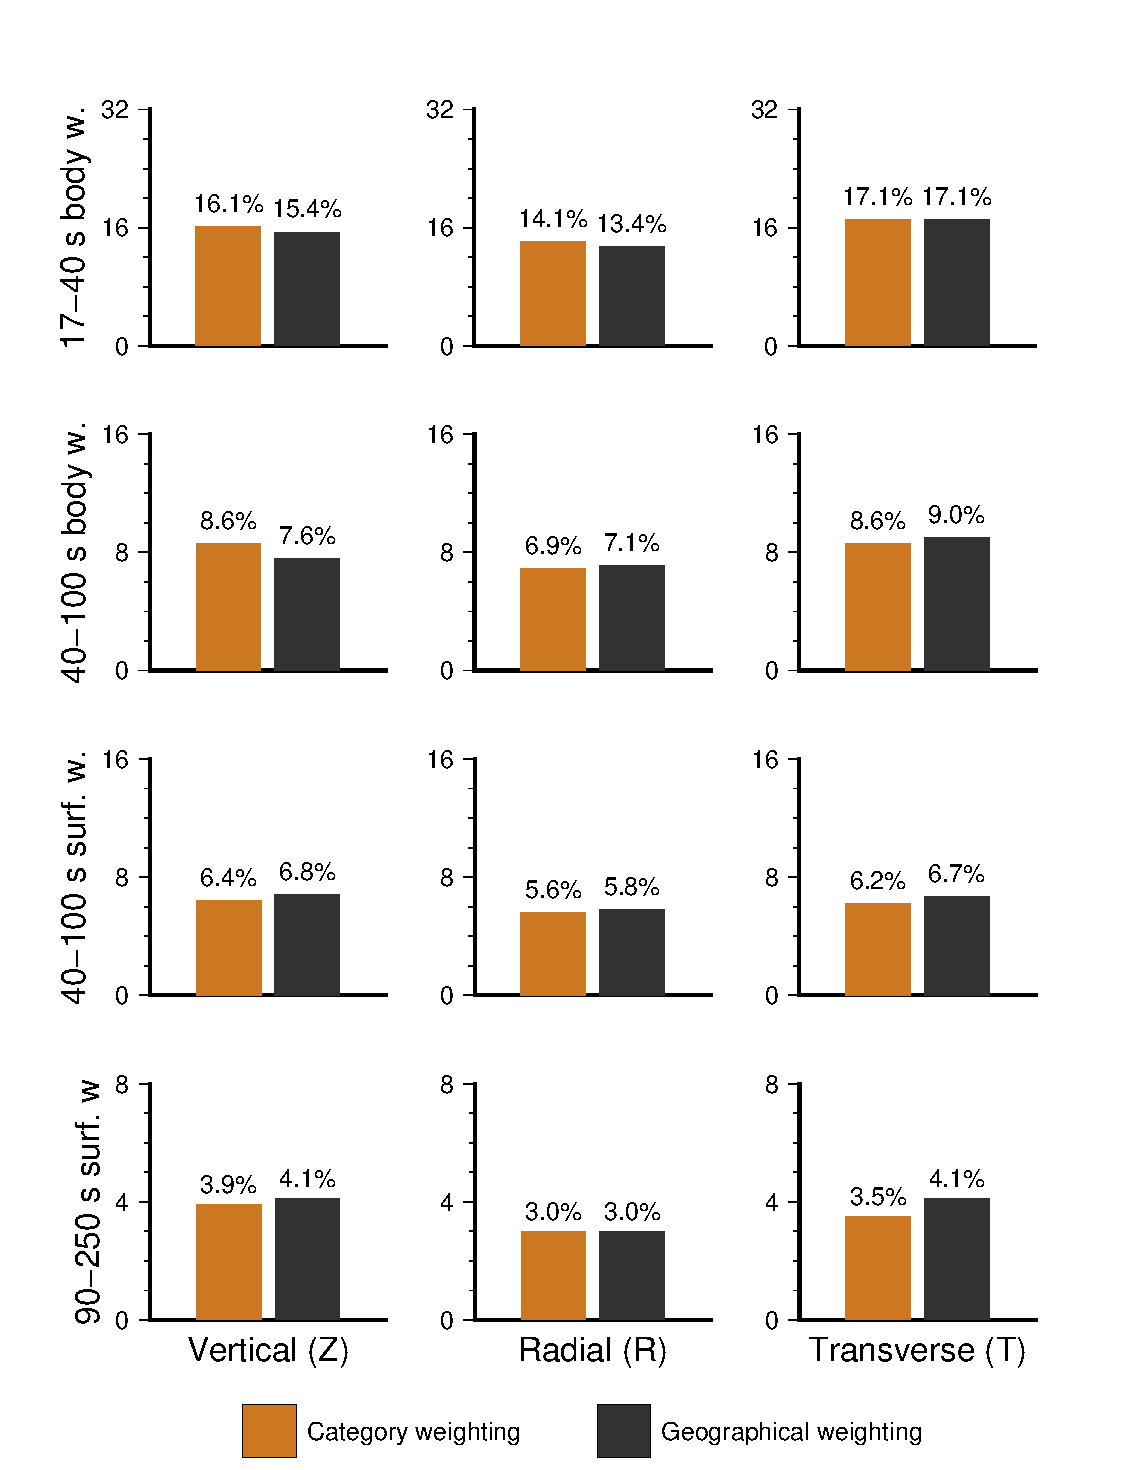
\includegraphics[width=0.8\textwidth]{ch-weighting/figures/category_misfit_contribution_color.pdf} 
  \caption[Percentage of the misfit in twelve categories]
  {\small{Percentage of the misfit in each of the twelve categories (see Table~\ref{table:categories}) using the category-weighting strategy (orange),
and geographical-weighting 
strategy (black). The percentage contribution in each category is labeled above the bars. Note that each category's contribution to the misfit barely changes with geographical weighting, because weight re-balancing only happens within each category.
}}
\label{fig:weights_histogram}
\end{figure}

As described in Section~\ref{sec:dataproc}, the weight we assign to each measurement is the product of source, category, receiver, 
and window weights: $\omega_{s}\, \omega_{c} \,\omega_{scr}\, \omega_{scrw}$\,.
In Figures~\ref{fig:receiver_weights}~and~\ref{fig:source_weights},
we plotted weights~$\omega_{s}$ assigned to sources and weights~$\omega_{scr}$ assigned to receivers.  
Next, we examine the misfit when the product of all four weights is applied.  

In total, we picked more than 17 million windows from 1,480 sources and 12 categories~\cite{Lei2018}. 
As shown in Figure~\ref{fig:wcounts_contribution}, 
the contribution from each category is far from balanced.  Short period body-wave data (17--40 s)
account for more than 50\% of the total number of windows while long period surface waves (90--250 s) contribute less than 5\%.
Across all three periods bands, more than 80\% of windows correspond to body-wave data.  For a given period band, the vertical component always provides more 
data than the horizontals.
If not balanced, these differences between categories can cause regions 
sensitive to body waves to be updated more than regions sensitive to surface waves and slow down the overall convergence rate.    

We define the weighted misfit for each category as
\begin{equation}
\Phi_{c} = \sum_{s=1}^{S} \sum_{r=1}^{R_{sc}} \sum_{w=1}^{N_{scr}} \omega_s\, \omega_{c} \,\omega_{scr}\, \omega_{scrw}\, \chi_{scr}
\end{equation}
In Fig.~\ref{fig:weights_histogram}, we calculate the percentage of the summed misfit for each category 
using two weighting strategies: (1)~orange bars correspond to category-only weighting, and (2)~black bars correspond to the full category- and geographical-weighting strategy.

\begin{figure}
\centering
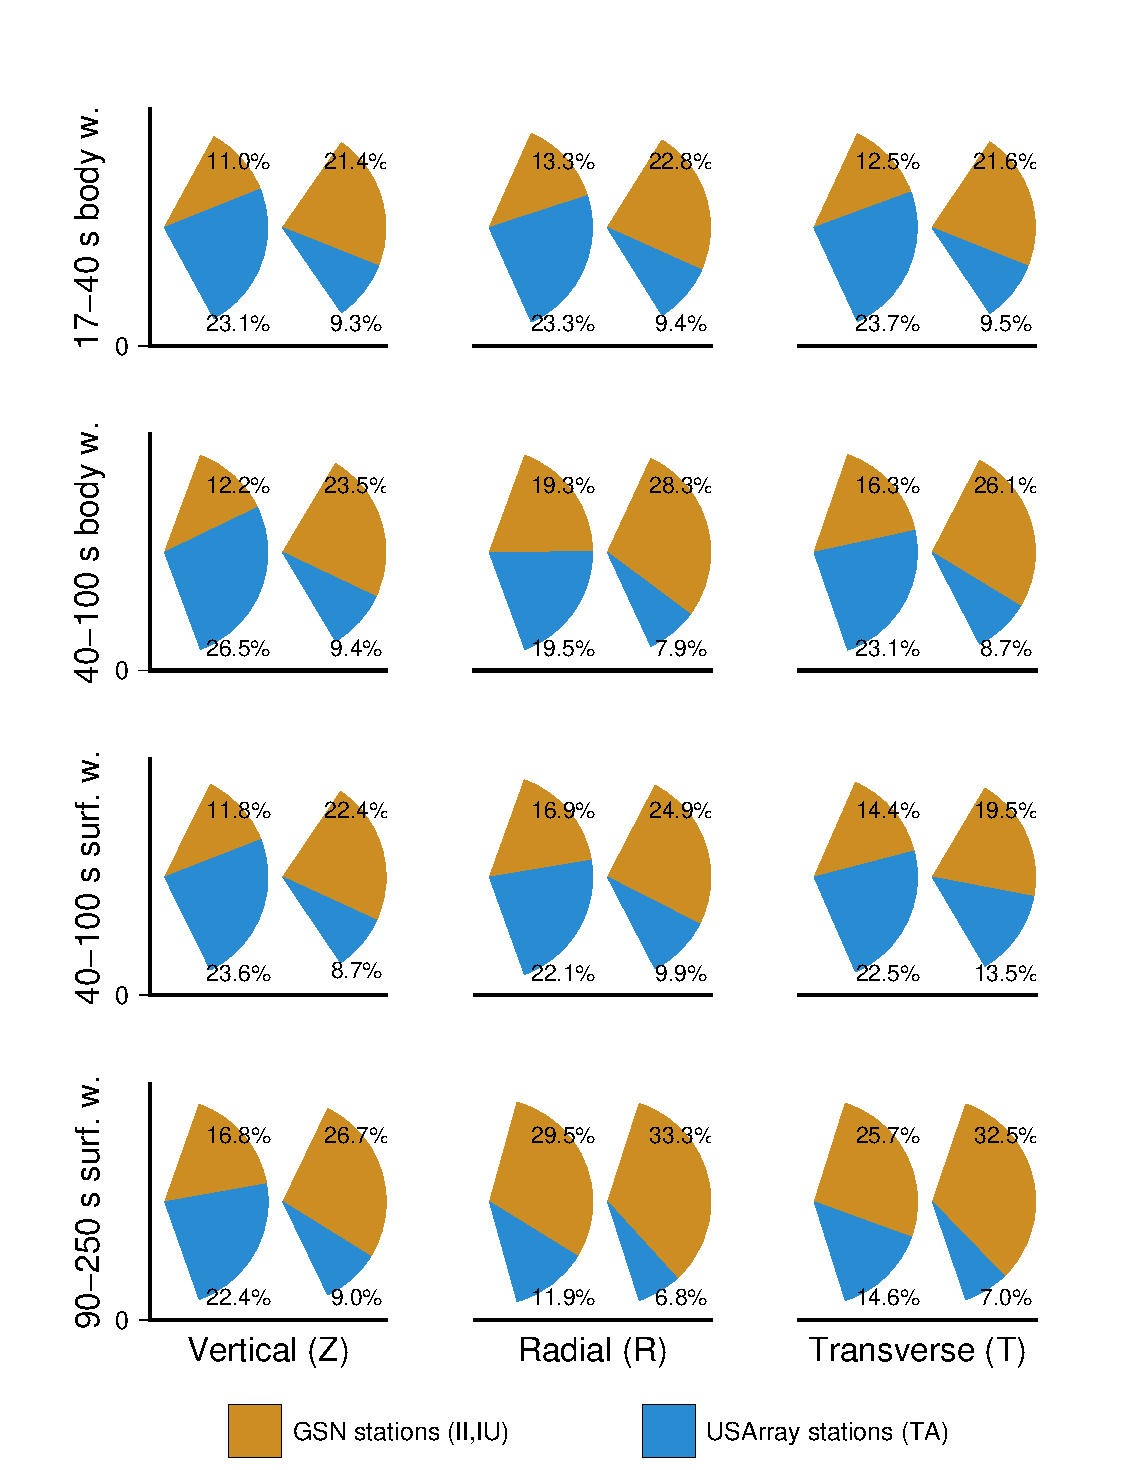
\includegraphics[width=0.85\textwidth]{ch-weighting/figures/category_sta_misfit_contribution.pdf}
  \caption[Percentage of the misfit of GSN stations and USArray stations]
  {\small{Percentage of the misfit of GSN stations (II, IU) and USArray stations (TA)
in each category using category-weighting (left wedges in each panel) and geographical-weighting
strategies (right wedges in panel).
Compared with the category-weighting strategy, the geographical-weighting 
strategy assigns more weight to GSN stations and down weights USArray stations in all categories.
}}
\label{fig:weights_contribution_sta}
\end{figure}

In the first case, after employing the category-weighting strategy in which the misfit is normalized by the 
total number of data in each category (Fig.~\ref{fig:wcounts_contribution}), misfits from different categories are better balanced 
and do not vary dramatically from category to category.  Although the 
summed weights themselves are equal in each category, the weighted misfits from each category 
are not.  The weighted misfits of short-period body waves are on average 2 to 3 
times larger than the misfits of long-period body and surface waves. We attribute this to the larger number of updates required to fit short-period phases compared with long-period phases, and we expect the body-wave misfits to decrease as the inversion progresses. 

In the second case, when geographical weighting is applied, the distribution of 
misfits in each category does not significantly change, meaning that the  re-balancing happens only within each category, as desired.

To further probe the overall re-balancing within each category, we compare the contribution to the total misfit from  two seismographic networks:  USArray (network ID TA) and GSN (network IDs II and IU).
USArray stations are densely distributed across North America and GSN stations are sparsely distributed across the  globe.

The total  misfit from USArray or GSN stations in each category is given by
\begin{equation}
\Phi_{c}^{\text{\scriptsize USArray / GSN}} = \sum_{s=1}^{S} \sum_{r=1}^{R_{sc}} \sum_{w=1}^{N_{scr}} \omega_s\, \omega_{c}\, \omega_{scr}\, \omega_{scrw}\,\chi_{scr}^{\text{\scriptsize USArray / GSN}}
\end{equation}
Fig.~\ref{fig:weights_contribution_sta} shows the percentage of~$\Phi_{c}^\text{\scriptsize USArray}$ and  
$\Phi_{c}^\text{\scriptsize GSN}$ in each category under different weighting strategies.
In the category-weighing strategy, GSN stations contribute much less to the overall misfit than  
USArray stations, reflecting the proportionality to the amount of data, as expected.
In the geographical-weighting strategy, the contribution 
of GSN stations is enhanced due to the re-balancing. 

\begin{figure}
\centering
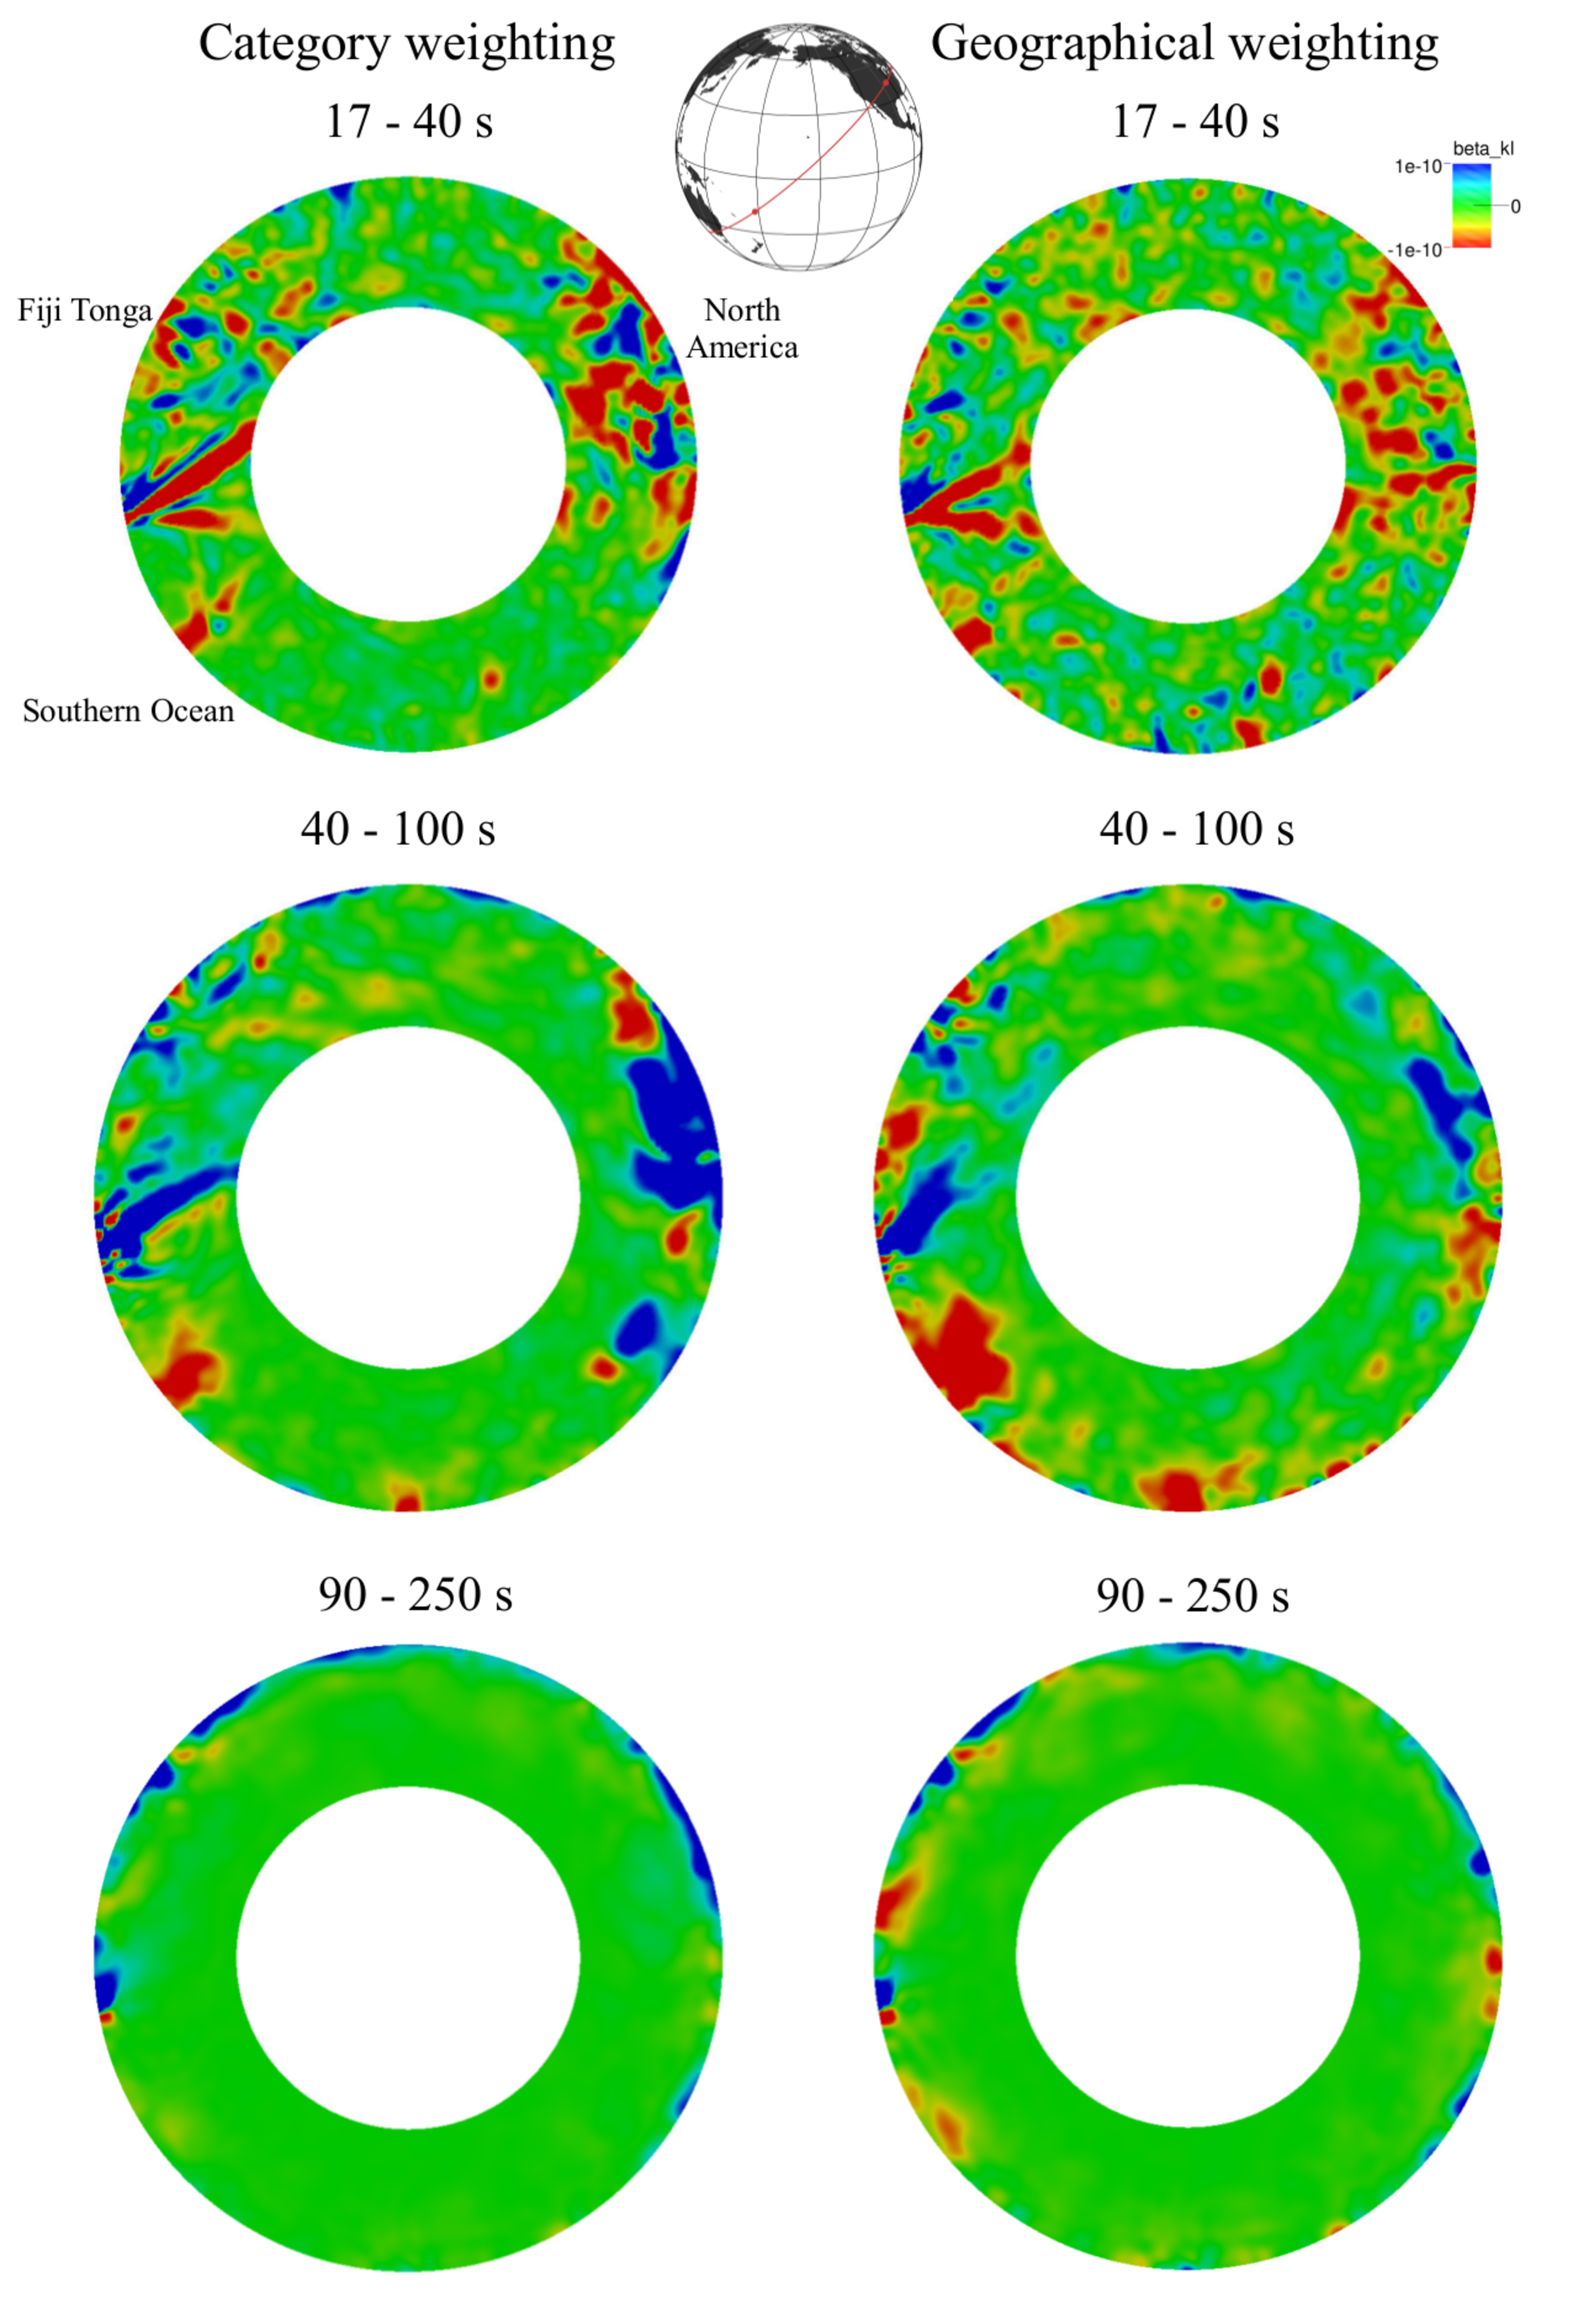
\includegraphics[width=0.85\textwidth]{ch-weighting/figures/Figure-10-small.pdf}
  \caption[Smoothed gradient contributions w/ and w/o weightings applied]
  {\small{Smoothed gradient contributions using data from 42 earthquakes without (Left Column) 
and with source \& receiver weighting (Right Column) in three
period bands: 17--40~s (Top Row), 40--100~s (Middle Row), and 90--250~s (Bottom Row). The top center map shows the cross section with red line for reference.   
The isotropic smoothing length scale is 100~km.
}}
\label{fig:gradient_category}
\end{figure}

To further illustrate the effects of weighting, we selected 42 events for a 
pilot test and examined the model update gradient. Ideally, we should run forward and adjoint simulations for 
each of the 12 categories for one weighting strategy, and repeat this process for the other weighting strategy, which would require 2,016
simulations in total.
To save computational cost while keeping the test meaningful,
we considered only three categories, 17--40~s, 40--100~s, 
and 90--250~s, and ignored wave types for the adjoint simulations. 
Fig.~\ref{fig:gradient_category} shows cross sections of the model update gradient.
In the shortest period band (17--40~s),
the gradient based on category-weighting is
dominated by regions beneath Fiji Tonga and North America,
with limited updates in the southern hemisphere.
In contrast, the geographical-weighting approach results in a balanced gradient with
more information in the southern hemisphere and relatively reduced sensitivity beneath Fiji Tonga and North America.  
The longer period bands, involving mostly surface waves,
demonstrate similar behavior but more focused on the shallow mantle.  
Upon combining all three categories, we clearly see that the model update based on the geographical 
weighting strategy is better balanced, with a more even sampling of the whole mantle (Fig.~\ref{fig:gradient_sum}).  
From this pilot test we conclude that the geographical-weighting strategy effectively 
balances the inversion and improves the convergence rate, which is necessary for any inversion dealing 
with the unevenly distributed data.

\begin{figure}
\centering
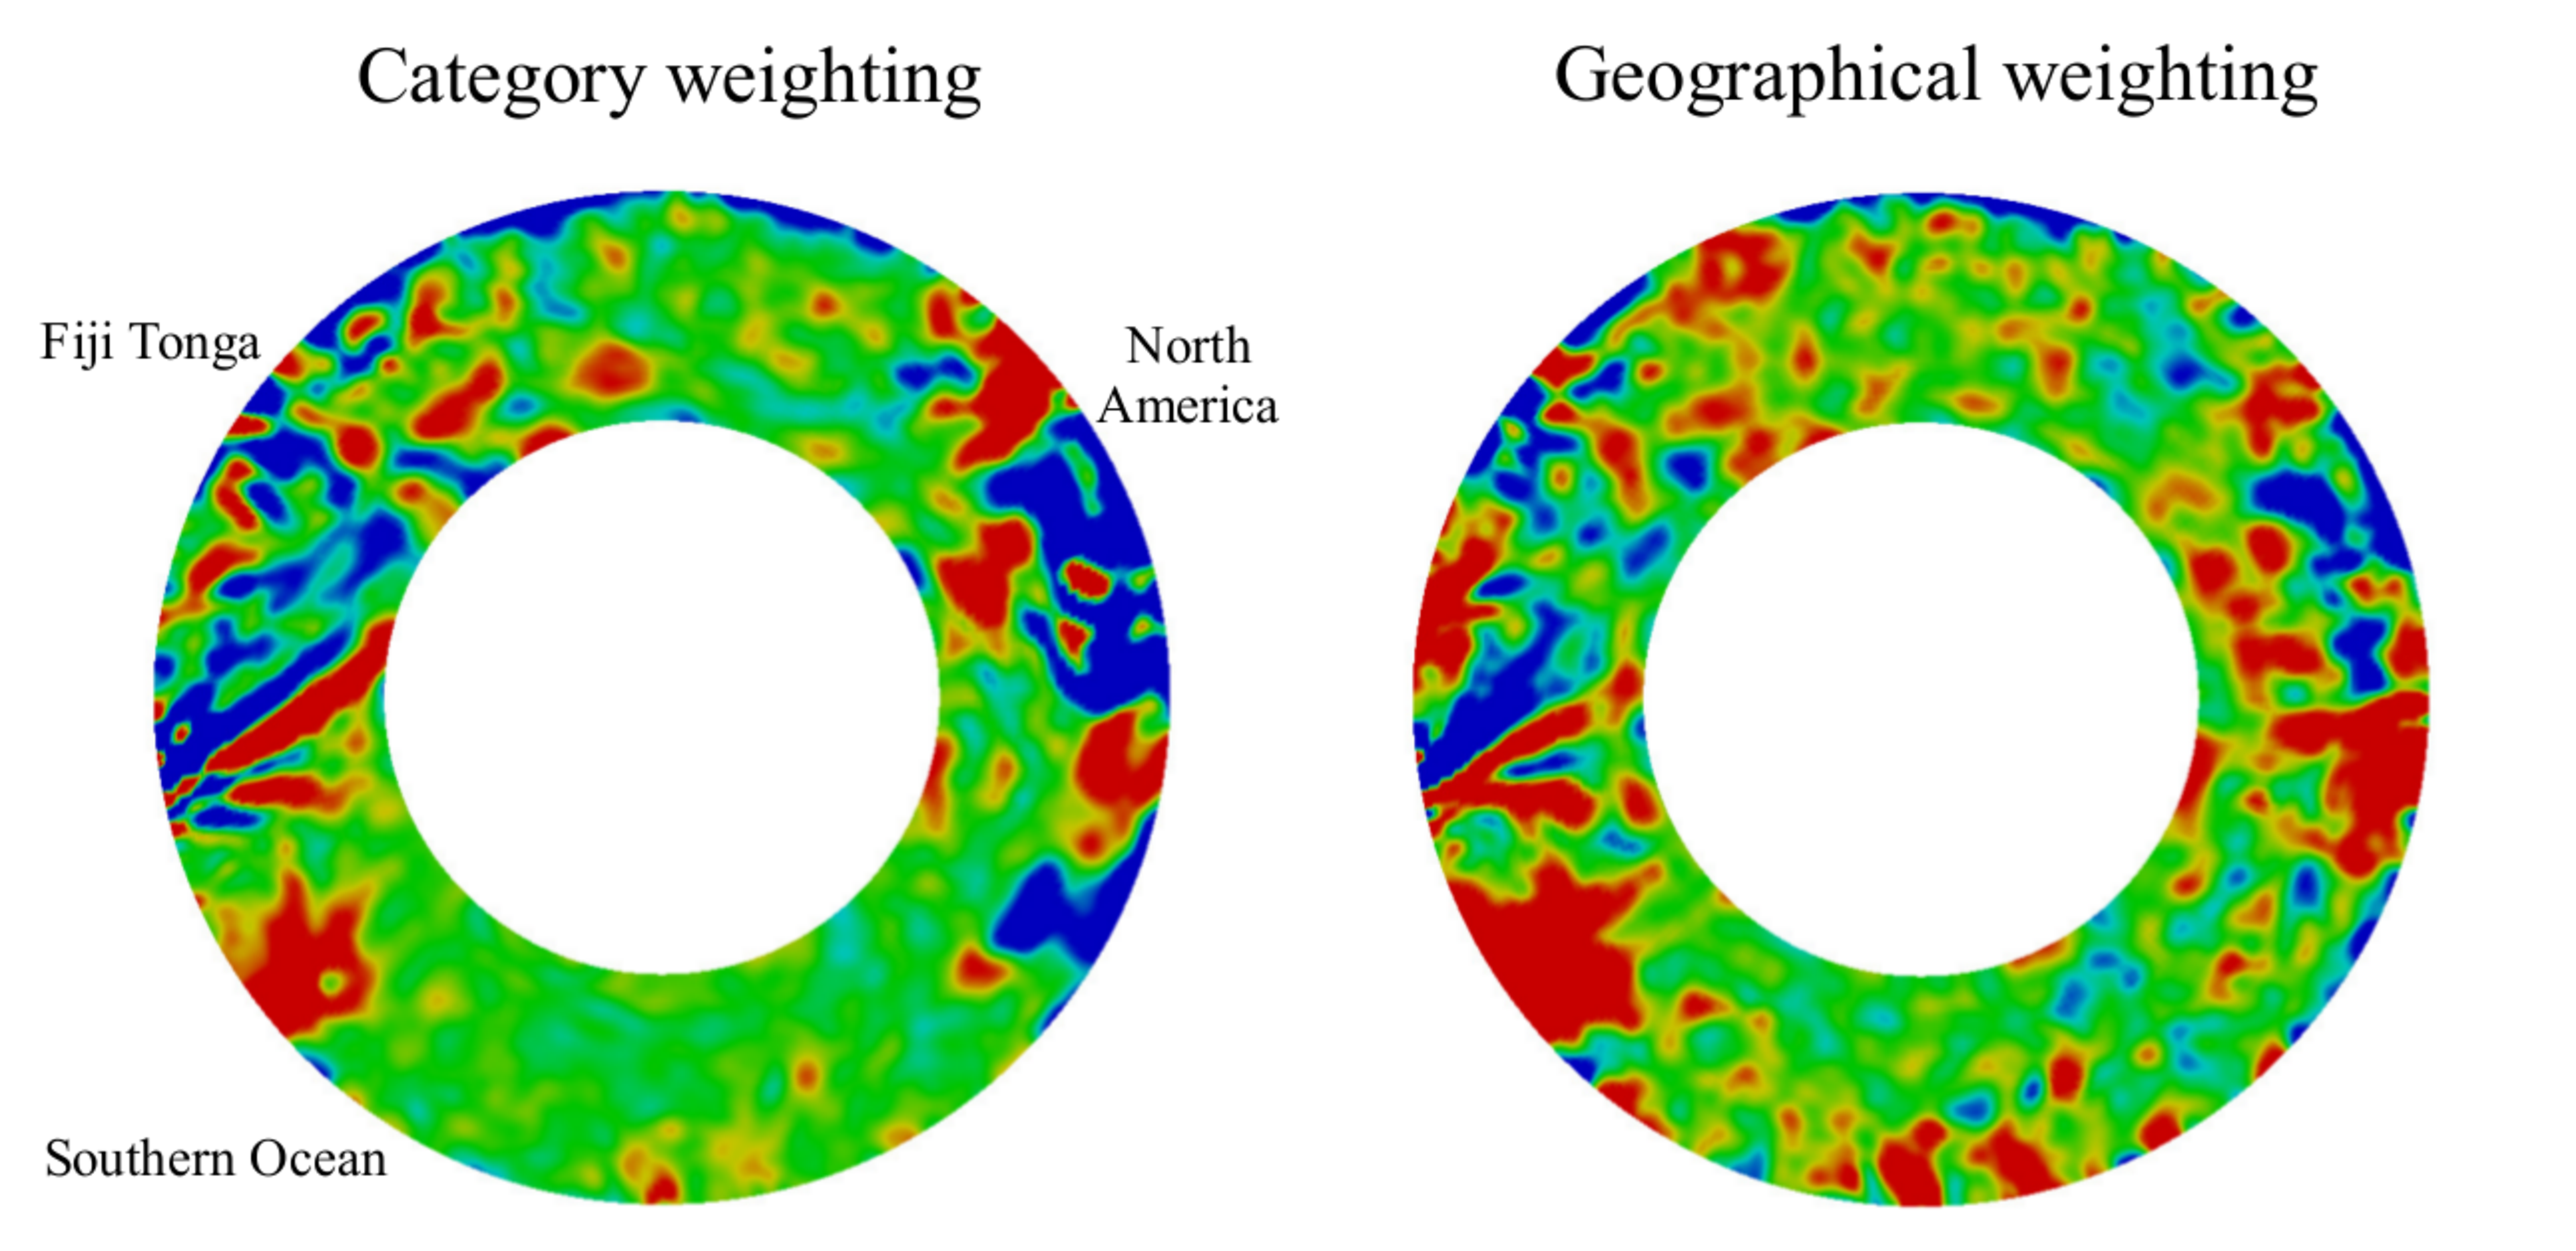
\includegraphics[width=0.85\textwidth]{ch-weighting/figures/Figure-11-small.pdf}
  \caption[Example of the summation of smoothed misfit gradients from three period bands]
  {\small{Example of a smoothed misfit gradient (weighted summation of the contributions of the three period bands shown in Fig.~\ref{fig:gradient_category}) 
using data from 42 earthquakes without (Left) and with source \& receiver weighting (Right). The isotropic smoothing length scale is 100~km.
}}
\label{fig:gradient_sum}
\end{figure}

% \subsection{Weighting double-difference Measurements}
% The geographical-weighting strategy introduced above can be adapted to other scenarios with uneven 
% data coverage. For instance, in the double difference inversion~\citep[e.g.,][]{Yuan2016} where the difference between 
% station are used as the misfit, a dense regional array will have many more station pairs than individual stations, 
% the inversion can suffer from even greater lopsidedness than conventional ones.  The station weights introduced in Section~\ref{sec:geographical_weights} (Top in Fig.~\ref{fig:dd_weights} for reference) can be adapted 
% to double difference case.  To address the unevenness of data coverage in double-difference inversion,
% we introduce an additional term~$P_{csi}$, the number of the station pairs associated with a single station, to balance the 
% contribution of station pairs. The geographical distribution of not individual stations but rather of stations pairs then 
% leads to a modified receiver weighting,
% \begin{equation}
% 	\omega_{csr} = \left( \sum_{i=1}^{R_{cs}} P_{csi} \exp\left[\mbox{}-\left(\frac{\Delta_{ir}}{\Delta_{0}}\right)^2\right] \right)^{-2} \quad ,
% \label{eq:dd_weights}
% \end{equation}
% where~$P_{csi}$ is the number of station pairs associated with the~$c$-th category,~$s$-th source, and~$i$-th receiver.  
% The normalizations and category weights described in Section~\ref{sec:norm} 
% remain the same in the double difference case as in the conventional case. 
% We note that in the limit of~$\Delta_{0} \to 0$, eqn.~\ref{eq:dd_weights} simply reduces to~$\omega_{csr} = P_{csr}^{-2}$. 
% In Fig.~\ref{fig:dd_weights},  we show the effect of the additional term in the receiver weighting.  The bottom plot shows
% that the additional term~$P_{csi}$ combine with the geographical-weighting produces larger contrast between 
% the weights of dense receivers and sparse receivers and therefore better address the unevenness in double-difference data.  
% More detail of the implementation of this weighting strategy and it's effect on the double-difference tomography is beyond the 
% scope of this paper and will be discussed in ({\color{Red} reference of Orsvuran et al.})

%%%%%-------------------------
%
%  conclusions
%
%%%%%-------------------------
\section{Conclusion}

We propose a geographic weighting strategy to address uneven data coverage in seismic tomography.  %We demonstrated how we introduce the weighting strategy while preserving the degree of freedom of the data. 
To test the approach, we performed synthetic 2D global adjoint tomography experiments using realistic source and receiver distributions.  
The results show that geographical weighting performs better than category-only weighting and conventional diagonal model-space preconditioning. %More importantly, it not only avoids pathological behavior along array-events but also achieves the results much faster and converges closer to the target. 
%The results also approve that the geographical-weighting can be a good approximation of a complete data covariance matrix.  
A 42-event pilot test was used to illustrate how  
geographical weighting balances densely and sparsely sampled regions.  
Finally,
using a database of 1,480 earthquakes, we performed a statistical analysis of 17~million measurements assimilated in the global adjoint tomography inversion of~\cite{Lei2018}, verifying expected effects of the weighting scheme. 
As more data from dense regional seismographic networks become available, we expect weighting to play an increasingly important role in scientific studies of Earth's interior~\cite{Orsvuran2019}.    

\chapter{Global Adjoint Tomography -- Model GLAD-M25\label{ch:GLAD-M25}}

\textbf{Note}\\
This chapter has been submitted as a paper entitled ``Global Adjoint Tomography -- Model GLAD-M25'' by Lei, W., Ruan, Y., Bozda\u{g}, E., Peter, D., Lefebvre, M., Komatitsch, D., Tromp, J., Hill, J.,  Podhorszki, N., and Pugmire, D.\ to the \textit{Geophysical Journal International}.

\section*{Summary}
Building on our first-generation global adjoint tomography model,
GLAD-M15~\cite{bozdaug2016global}, we present our second-generation transversely isotropic global model,
named GLAD-M25, which is the result of ten quasi-Newton tomographic iterations with an
earthquake database consisting of 1,480 events in the magnitude range $5.5\le M_w \le 7.2$,
an almost six-fold increase over the first-generation model.
We calculated fully 3D synthetic seismograms with a shortest period of 17~s based on a GPU-accelerated spectral-element wave
propagation solver which accommodates effects due to 3-D anelastic crust \& mantle structure, topography \& bathymetry, the ocean load, ellipticity, rotation, and self-gravitation.
We used an adjoint-state method to calculate Fr\'echet derivatives in 3D anelastic Earth models
facilitated by a parsimonious storage algorithm.
The simulations were performed on the Cray XK7 ``Titan'' at the Oak Ridge Leadership Computing Facility.
We quantitatively evaluated GLAD-M25 by assessing misfit reductions and traveltime \& amplitude anomaly histograms in twelve measurement
categories.
We performed similar assessments for a held-out data set consisting of 360 earthquakes,
with results comparable to the actual inversion.
We compare GLAD-M25 with numerous other global and regional models,
and highlight a variety of plumes and subduction zones.

\section{Introduction}

Construction of the first seismic tomographic models of the Earth dates back to the late 1970s~\cite{Aki77,Dziewonski77,SenTok77} and early 1980s~\cite{WD84, Nataf1984}.
Around the same time,
\cite{BaChLa77}, \cite{Lailly1983}, and~\cite{Tar84} formulated and adapted the theory of adjoint-state methods~\cite{Chavent1974} for exploration seismology with the goal of capturing the full physics of seismic wave propagation.
Mainly due to computational challenges,
it took until the late 2000s to see the first applications of adjoint-state methods in regional- and continental-scale earthquake seismology~\cite{tape2009adjoint,Fichtner09,zhu2012structure}.
The first global ``adjoint tomography'' model of the Earth's mantle,
GLAD-M15, was published in 2016~\cite{bozdaug2016global}, more than 30 years after the development of the original ``full waveform inversion'' (FWI) theory.

Current global seismic models are in general agreement regardless of data type and inversion strategy in terms of long-wavelength heterogeneity \cite{ritzwollerlavely1995,TW01,beckerboschi2002}.
However, discrepancies between models become noticeable as resolution increases.
Using accurate 3D simulations of seismic wave propagation and the computation of data sensitivities in 3D background models are key requirements for improving resolution in tomographic images on all scales.
Such detailed images are essential for understanding mantle dynamics and related surface tectonic processes
---for example the origin of hot-spots and the forces behind plate motions and earthquakes.
Higher resolution wavespeed models are also important for accurately locating earthquakes, and are required from an engineering point of view to assess seismic hazard in earthquake prone regions and to detect nuclear explosions. 

With these goals in mind,
in this study we use a GPU-accelerated version of the 3D spectral-element solver
SPECFEM3D\_GLOBE~\cite{KoTr02a,KoTr02b} on the Cray supercomputer ``Titan'' at the Oak Ridge Leadership Computing Facility (OLCF) for global adjoint tomography.
These simulations accommodate the full 3D complexity of global Earth models,
including 3D anelastic crust and mantle structure, self-gravitation, rotation, ellipticity, topography \& bathymetry, and the load of the oceans.
No compromises are made with regards to resolving the Earth's crust,
which is explicitly captured by the spectral-element mesh~\cite{tromp2010a},
thereby eschewing the need for ubiquitous ``crustal corrections''.
The ultimate goal is to use every single piece of information in seismograms,
a task made partly feasible based on the automated window selection tool FLEXWIN~\cite{maggi2009automated}.

Global adjoint tomography has a well-defined but complex workflow with multiple stages.
% including numerical simulations of synthetic seismograms (forward simulations) for all events,
% pre-processing of seismic data, making measurements, data assimilation, Fr\'echet derivative
% calculations (adjoint simulations), and post-processing of the gradient for quasi-Newton model
% updates.
It is essential to optimize, automate, and harden the entire process using workflow management tools, especially with large data sets.
For each iteration,
1,480 forward and adjoint simulations need to be performed,
generating a few Petabytes of wavefield files for the parsimonious-storage kernel calculation algorithm of~\cite{KoXiBoPeSaLiTr16}, and consuming 16~million OLCF node hours.
How to deal with hardware failures during this process is critical
to prevent contamination of the inversion results.
For these reasons, we use EnTK as our
workflow management engine~\cite{EnTK2017}.
This workflow engine can automatically detected job failures,
both from the high-performance computing (HPC) system and via user-defined functions.
This facilitates tracking of tasks and semi-automatic job resubmission if necessary.

In this article we compare the results of our inversion with a number of previous tomographic models.
On a global scale, we present comparisons with model S362ANI$+$M~\cite{moulik2014anisotropic},
which is an updated version of model S362ANI~\cite{kustowski2008anisotropic},
the starting model for the GLAD-M15 inversion.
We also consider global shear wavespeed models S40RTS~\cite{ritsema2011s40rts},
TX2015~\cite{TX2015}, SEMUCB-WM1~\cite{french2015broad},
and SL2013sv~\cite{SchaefferLebedev13},
as well as compressional wavespeed models LLNL-G3Dv3 \cite{simmons2012llnl}, GAP-P4~\cite{fukao2013subducted}, and UU-P07~\cite{van2018atlas}.
On the scale of North America
we make comparisons with models US22~\cite{zhu2017radial},
a radially anisotropic model based on adjoint tomography using USArray data from 180 regional earthquakes,
and SL2013NA~\cite{schaeffer2014imaging},
a modification of global model SL2013sv focused on North America.
In Europe we use regional model EU60~\cite{zhu2015seismic} for comparison,
which is based on the assimilation of data from 190 regional earthquakes recorded by more than 700 European seismographic stations.
Finally, in Asia we use regional adjoint tomography model EARA2014~\cite{chen2015multiparameter} as a reference, a model based on data from 227~earthquakes recorded by more than 1,800~stations.

This article is organized as follows.
Sections~\ref{section:start}--\ref{section:data} describe the starting model,
earthquake database, and seismographic data set. 
Sections~\ref{section:misfit} and~\ref{section:parameterization} describe the misfit function minimized during the inversion process
and the related model parameterization.
In Section~\ref{section:workflow} we describe the adjoint tomography workflow in some detail.
Section~\ref{section:misfit_evolution} describes the evolution of the misfit, and in Section~\ref{section:evaluation} we evaluate the model based on a held-out data set of 360 earthquakes.
Finally, in Section~\ref{section:model}, we describe the model in detail,
offering many comparisons with various global and regional models, as described in the proceeding paragraph.
We conclude with a discussion of future opportunities and directions.

\section{Starting model GLAD-M15}
\label{section:start}

As a continuation of our previous work~\cite{bozdaug2016global},
we used the first-generation model GLAD-M15 as our
starting model.
GLAD-M15 is a 3D transversely isotropic earth earth model, which combined
3D mantle model S362ANI~\cite{kustowski2008anisotropic}
with 3D crustal model CRUST2.0~\cite{bassin2000current} as its starting model.
In this study,
we continue to use the same transversely isotropic model parameterization.
Instead of relying on crustal corrections,
the mesh implementation of the crust in the spectral-element solver SPECFEM3D\_GLOBE~\cite{KoTr02a,KoTr02b,PeKoLuMaLeCaLeMaLiBlNiBaTr11} enables us to accurately accommodate topography and bathymetry as well as variations in the Moho.
GLAD-M15 was constructed using a global database of 253 earthquakes.
The first 12 iterations of the GLAD-M15 inversion used three-component seismograms with a shortest period of 27~s,
and the final 3 iterations reduced this further to 17~s.
In this study we also used three-component seismograms with a shortest period of 17~s.

\section{Earthquakes}
\label{section:earthquakes}

\begin{figure}
  \centering
  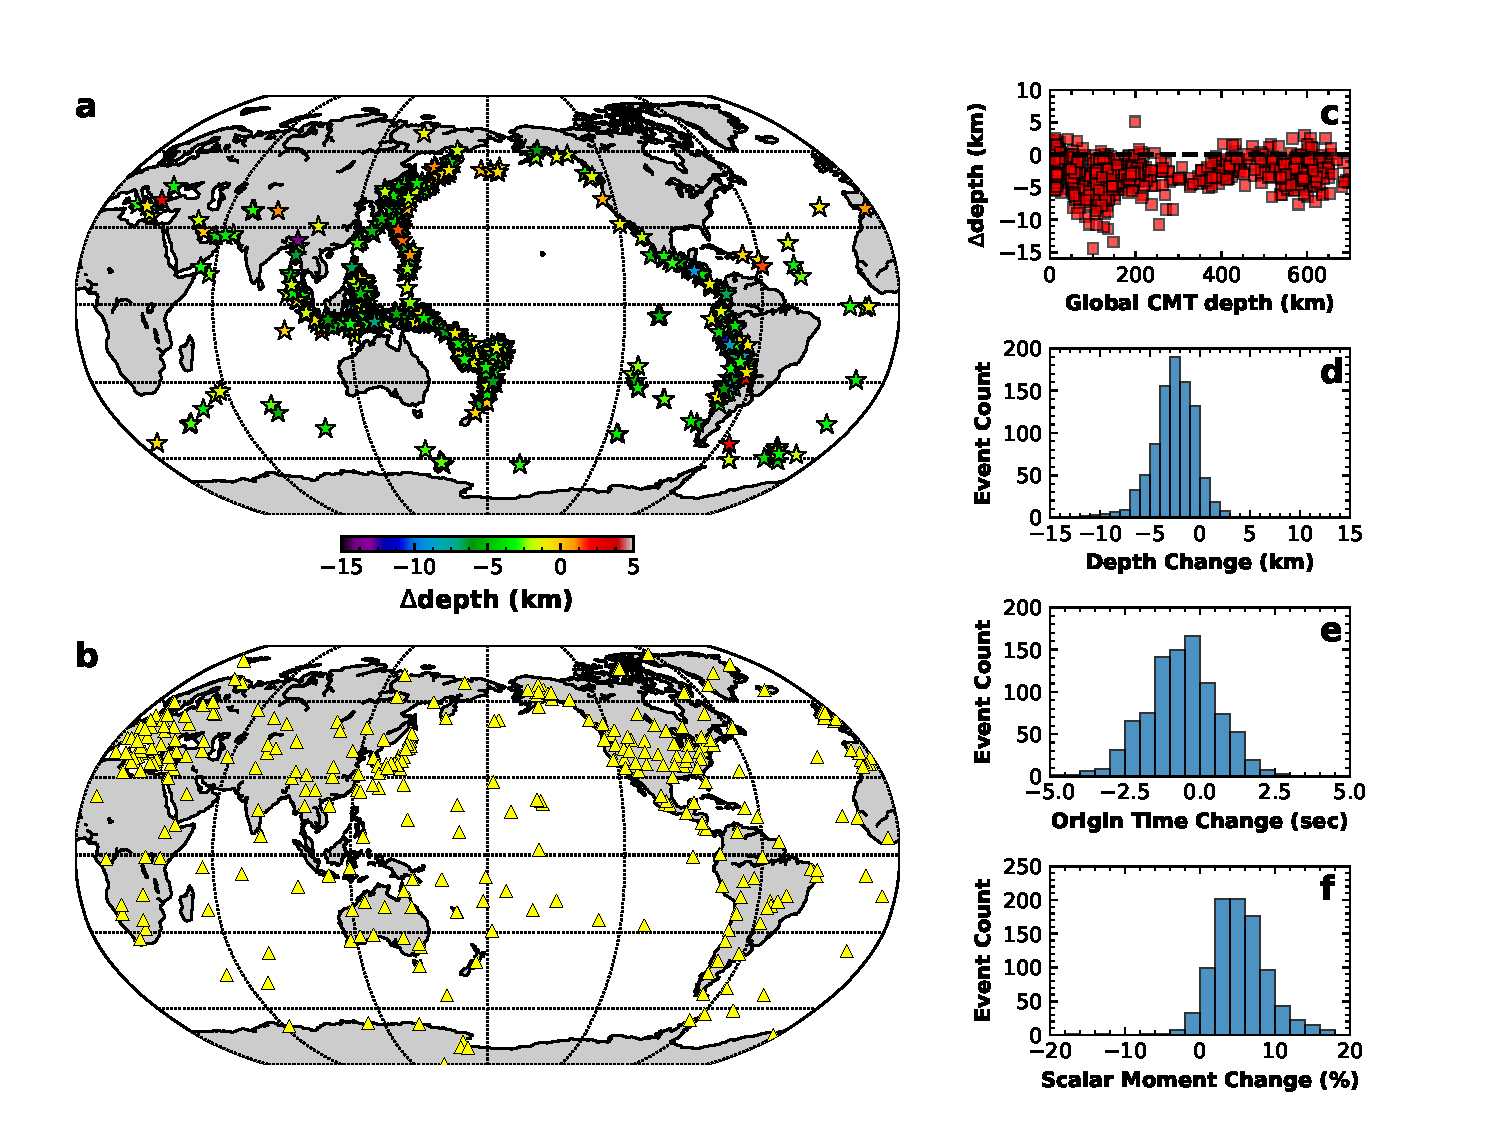
\includegraphics[width=\textwidth]{ch-GLADM25/figures/source_corrections.pdf}
  \caption[Source corrections for 1,040 events]
  {\small{Source corrections for 1,040 out of 1,480 events used in the structural inversion. (a)~Map view of depth changes. (b)~Distribution of seismographic stations used for source inversions. (c)~Depth change relative to the original global CMT Catalog depth. (d)--(f)~Histograms of depth, origin time, and scalar moment changes relative to the CMT Catalog.
  }}
  \label{fig:source_correction}
\end{figure}

In addition to the 253 earthquakes used for the construction of GLAD-M15, we initially carefully selected 784 additional earthquakes
from the global Centroid-Moment Tensor (CMT) catalog~\cite{ekstrom2012global},
resulting in a total number of 1,040 earthquakes.
To ensure a good signal-to-noise ratio on a global scale,
the smallest moment magnitude in the database is set to~5.5,
thereby capturing more deep events,
and, to avoid complications associated with source dimension and directivity,
the largest moment magnitude is set to~7.2.

Before using the 1,040 earthquakes in our structural inversion,
we performed CMT inversions using model GLAD-M15,
the results of which are summarized in Fig.~\ref{fig:source_correction}.
To ensure even global coverage,
we used seismographic stations from the  Global Seismic Network (II, IU, IC, US, CU, and GT),
GEOFON~(GE), GEOSCOPE~(G), and several regional networks, such as MedNet~(MN),
the Brazilian Lithospheric Seismic Project~(BL), the Chilean National Seismic Network~(C),
and the Japan Meteorological Agency Seismic Network~(JP) (Fig.~\ref{fig:source_correction}b).
The number of stations used for CMT inversion usually ranges
from~150 to~500.

To determine the source parameters in the starting model,
we used the CMT inversion algorithm of \cite{liu2004spectral}.
This algorithm combines a normalized waveform difference misfit with an envelope difference misfit.
Specifically, the algorithm minimizes the misfit function
\begin{equation}
   \begin{split}
      \Phi =  \sum\limits_{c=1}^{C} \omega_c \sum\limits_{r=1}^{R_c} \omega_{cr}
       \sum\limits_{w=1}^{W_{cr}} \omega_{crw}\,
          & \left\{ \lambda\, \frac
              { \int \big[ d_w(t) - s_w(t - \Delta t) \big]^2 \mathrm{d}t}
              {\int \big[ d_w(t) \big]^2  \mathrm{d}t} \right.
       \\ & \quad \left. \mbox{} + (1 - \lambda)\, \frac
              {\int \big[ e(d_w(t)) - e(s_w(t - \Delta t)) \big]^2 \mathrm{d}t}
              {\int \big[ e(d_w(t)) \big]^2\mathrm{d}t} \right\}
              \quad ,
   \end{split}
\end{equation}
where~$d_w(t)$ denotes data in time window~$w$\,,
and~$s_w(t - \Delta t)$ the corresponding synthetic for model~GLAD-M15.
We allow the synthetics to shift relative to the data by an amount~$\Delta t$
--- effectively a station correction --- determined by cross correlation.
The envelope function is denoted by~$e(\,\cdot\,)$\,,
and the parameter~$\lambda$ determines the balance between fitting waveforms versus fitting envelopes.
The number of measurement categories is denoted by~$C$\,.
Following~\cite{ekstrom2012global},
seismograms were filtered between 50~s and 100~s
to select three-component body-wave windows,
and between 60~s and 100~s to select three-component
surface-wave windows,
resulting in six measurement categories, $c=1,\ldots,C$\,.
To balance their contributions,
each category is weighted by the reciprocal of the number of measurements in that
category, $\omega_c$\,.
The number of windows for a given receiver~$r$ in a given measurement category~$c$ is~$W_{cr}$\,.
Each such window is weighted equally, i.e.,~$\omega_{crw}=1$\,.
The number of receivers that records data in category~$c$ is denoted by~$R_c$\,.
As shown in Fig.~\ref{fig:source_correction}b,
the receivers are unevenly distributed across the globe,
with several dense arrays in the Northern Hemisphere and poor coverage in the Southern Hemisphere.
To balance the coverage,
following a strategy articulated by~\cite{Ruanetal2018},
we assign receiver weights~$\omega_{cr}$ based on the expression
\begin{equation}
\omega_{cr}^{-1} = N_c\,\sum_{r'=1}^{R_c} \exp\left[\mbox{}-\left(\frac{\Delta_{rr'}}{\Delta_c}\right)^2\right]
\quad ,
\label{eq:spatial_weights1}
\end{equation}
where~$N_c$ is a normalization factor for category~$c$,
and where~$\Delta_{rr'}$ denotes the angular distance between receivers~$r$ and~$r'$\,.
The reference angular distance~$\Delta_c$ for each category~$c$ needs to be chosen such that the condition 
number of the diagonal weighting matrix defined by Eqn.~(\ref{eq:spatial_weights1}) is not too large.
The calculation of the weights may be abstracted as: given a distribution of
points on the unit sphere, determine a spatial weighting associated with each point.

The algorithm inverts for the six elements of the moment tensor
and the centroid location~(latitude, longitude, and depth).
These source inversions are computationally very expensive,
because for each of the 1,040~events nine full 3D forward simulations are required to obtain the source parameter Fr\'echet derivatives.

Because we allow the synthetics to shift in phase by an amount~$\Delta t$ relative to the data,
the CMT inversion has unreliable sensitivity to the centroid time.
To alleviate this problem,
following~\cite{zhu2012structure},
we perform a subsequent grid search for the centroid time and the scalar moment.
The grid-search calibration involves simple shift and multiply operations on seismograms
and, unlike the CMT inversion, requires minimal simulation time.

Most earthquakes show a shallower depth after inversion
(Fig.~\ref{fig:source_correction}c),
consistent with our previous experiences~\cite{zhu2015seismic,chen2015multiparameter,bozdaug2016global} and with experiments by~\cite{hjorleifsdottir2010effects}.
We observed an average depth change of~$-2.62\pm2.49$~km relative to the global CMT solutions,
an average scalar moment change of~$5.31\pm3.91$\%,
and an average centroid time shift of~$-0.60\pm1.17$~s.
These are relatively minor corrections, especially in view of the significant expense of the source inversions.
For this reason, when we added another 440 earthquakes during iteration~22,
thereby bringing the total to~1,480 events,
we only performed a grid search to calibrate the centroid times and scalar moments.
Fig.~\ref{fig:event_1480} summarizes the characteristics of all 1,480 earthquakes used in this study.

\begin{figure}
  \centering
  \includegraphics[width=\textwidth]{ch-GLADM25/figures/events_1480.pdf}
  \caption[The distribution of 1,480 earthquakes used in structural inversion]
  {\small{The 1,480~earthquakes used in this study. (a) Distribution of earthquakes. The color of each beach ball reflects its depth range, where blue designates events shallower than 50~km, green events between 50~km and 300~km, and red events deeper than 300~km. (b) \& (c) Histograms of earthquake moment magnitudes and depths.}}
  \label{fig:event_1480}
\end{figure}


\section{Seismic data}
\label{section:data}

The seismographic stations used in this study were carefully selected to ensure global coverage
and high data quality (Fig.~\ref{fig:stations}).
In addition to the seismographic  stations used for the source inversions,
we included all available data for our 1,480 event earthquake database from many data centers,
including IRIS, ORFEUS, INGV, IPGP, ETH, and GEONET.
Regional and temporary networks,
such as US Array~(TA),
Africa Array~(AF), the Canadian National Seismograph Network~(CN), Geoscience Australia~(AU),
the Antarctic Seismographic Argentinean Italian Network~(AI),
and the New Zealand National Seismograph Network~(NZ),
constitute a significant part
of our database and greatly improve coverage in certain regions.

\begin{figure}
  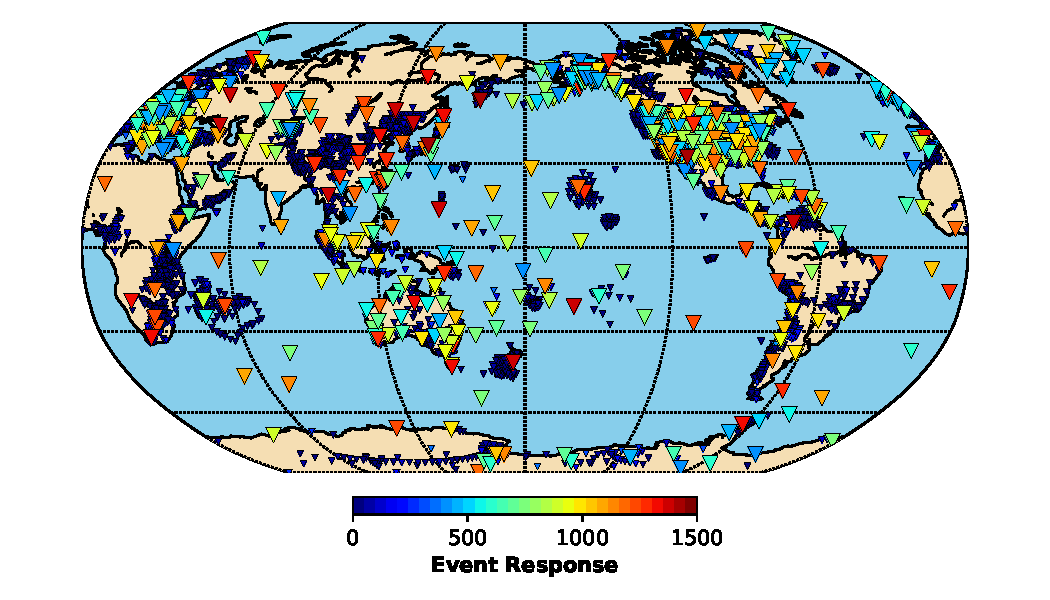
\includegraphics[width=0.8\textwidth]{ch-GLADM25/figures/station_map.pdf}
  \caption[Distribution of the seismographic stations]
  {\small{Distribution of the 11,800~seismographic stations used in this study. Colors denote the number of events for which a given station contributes waveforms to the structural inversion. Stations with a number of event responses $<400$ are plotted in smaller size; these are usually temporary arrays deployed over a short period of time, frequently ocean bottom seismometers. The maximum number of event responses comes from ANMO, in Albuquerque, New Mexico, which contributed to 1,442 out of 1,480 earthquakes in the data set.}}
  \label{fig:stations}
  \centering
\end{figure}

\subsection{Adaptable Seismic Data Format}
\label{section:ASDF}

Conventional seismic data formats, such as SAC, involve one file per time series
plus related files with instrument response and event information.
Since every earthquake in the database is typically recorded by thousands of
instruments, I/O during the preprocessing stage of the adjoint tomography workflow
quickly cripples the file system. The Adaptable Seismic Data Format
(ASDF)~\cite{krischer2016adaptable}
was developed with complete reproducibility and fast parallel processing in mind.

In this context, there are four key issues ASDF resolves.
\begin{itemize}
    \item Robustness and stability: the data container is developed and maintained to ensure accuracy of scientific results.
    \item Data organization: the container is self-describing. Data, including waveform, source, and station information, are organized into well-defined structures.
    \item Reproducibility: the container enables scientists to keep track of which operations have been performed on the data so that results can be reproduced.
    \item Efficiency: the format provides easy mechanisms for parallel processing.
\end{itemize}

ASDF serves as a self-contained-and-explained data container while taking
full advantage of parallel computing. In our workflow,
one ASDF file contains all the information needed for processing one event,
including the seismic traces, an event information file (in QuakeML format), and station response files (in StationXML format).
The related Application Programming Interfaces (API)s are carefully designed for easy data extraction and parallel processing.

\section{Misfit function}
\label{section:misfit}

The misfit function to be minimized during the iterative inversion process must
be carefully constructed.
In this study,
it typically involves cross-correlation traveltimes
for body waves and frequency-dependent multitaper phase measurements for surface waves.
Measurements are made in several passbands of three-component seismograms rotated
into vertical, radial, and transverse components, resulting in a number of measurement
categories.
In this study, we consider four passbands, namely, a 17--40~s passband targeting body waves,
two 40--100~s passbands separately targeting body and surface waves,
and a 90--250~s passband targeting longer-period surface waves.
Each passband involves measurements on all three components,
which results in a total of twelve measurement categories.
Although the inversion is designed to minimize the overall misfit,
we track the misfit reduction in each of the categories to ensure that
the model is improving the fit to the data roughly equally across the board.
One of the biggest challenges in the construction of the misfit function is the
highly uneven distribution of earthquakes --- discussed in Section~\ref{section:earthquakes} --- and seismographic stations,
which must be counterbalanced by geographically weighting the data.
This issue is discussed in detail by~\cite{Ruanetal2018};
in this section we present a brief synopsis.

With these considerations in mind,
the overall misfit, $\Phi$, is defined as follows:
\begin{equation}
\label{eq:misfit1}
\Phi = \sum_{s}^{S} \omega_s \sum_{c}^{C} \omega_{c} \sum_{r}^{R_{sc}} \omega_{scr} \sum_{w}^{W_{scr}} \omega_{scrw}\, \chi_{scrw}
\quad ,
\end{equation}
where~$S$ denotes the number of sources, $C$ the number of categories,
$R_{sc}$ the number of receivers recording source~$s$ in category~$c$,
and~$W_{scr}$ the number of measurement windows for source~$s$, category~$c$,
and receiver~$r$.
The misfit for a specific source~$s$, category~$c$, receiver~$r$, and window~$w$ is
\begin{equation}
  \chi_{scrw} = \frac{1}{\Delta\omega}\int_{\omega_1}^{\omega_2} \Big( \frac {\Delta \tau_{scrw}} {\sigma_{scrw}} \Big)^2\, \mathrm{d}\omega
\quad ,
\end{equation}
where~$\Delta \tau_{scrw}$ denotes a multi-taper frequency-dependent phase measurement over the frequency interval~$\Delta\omega=\omega_2-\omega_1$\,,
with associated uncertainties~$\sigma_{scrw}$\,.
For body waves, the window misfit is often simply the cross-correlation traveltime anomaly,
$\Delta T_{scrw}$\,, weighted by its standard deviation, i.e., $\chi_{scrw}=(\Delta T_{scrw}/\sigma_{scrw})^2$\,.
As in the source inversions,
the window weights are equal, $\omega_{scrw}=1$\,,
and the category weight, $\omega_c$\,, is the reciprocal of the number of measurements in that
category, $1/C$.
Earthquakes mainly occur along plate boundaries,
and most seismographic  stations are confined to the continents,
which leads to a very uneven distribution of sources and stations,
as illustrated in Figs.~\ref{fig:event_1480} and~\ref{fig:stations}.
Therefore, weighting is crucial in global tomography to balance this uneven sampling
of Earth's interior.
Our source and receiver weighting strategy,
encapsulated by the weights~$\omega_s$ and $\omega_{scr}$\,,
is developed to compensate for uneven spatial sampling.
Following the same strategy as for the receiver weights in the source inversions,
we define source and receiver weights as
\begin{equation}
\omega_{s}^{-1} = N\,\sum_{s'=1}^{S} \exp\left[\mbox{}-\left(\frac{\Delta_{ss'}}{\Delta}\right)^2\right]
\quad ,
\label{eq:source_weights}
\end{equation}
and
\begin{equation}
\omega_{scr}^{-1} = N_{sc}\,\sum_{r'=1}^{R_{sc}} \exp\left[\mbox{}-\left(\frac{\Delta_{rr'}}{\Delta_{sc}}\right)^2\right]
\quad ,
\label{eq:receiver_weights}
\end{equation}
respectively.
Here~$N$ and~$N_{sc}$ are normalization factors,
and~$\Delta_{ss'}$ and~$\Delta_{rr'}$ denote angular distances between source and receiver pairs~$\{s,s'\}$ and~$\{r,r'\}$\,.
The reference angular distances~$\Delta$ and~$\Delta_{sc}$ need to be chosen based on the condition 
numbers of the diagonal weighting matrices defined by Eqns.~(\ref{eq:source_weights}) and~(\ref{eq:receiver_weights}).

\section{Model parameterization}
\label{section:parameterization}

We use the same transversely isotropic model parameterization as starting model GLAD-M15.
Such a model is described by the five Love parameters $A$, $C$, $L$, $N$, and $F$~\cite{Love27},
or, alternatively, using the mass density~$\rho$, in terms of the wavespeeds~$\alpha_v=\sqrt{C/\rho}$, $\alpha_h=\sqrt{A/\rho}$, $\beta_v=\sqrt{L/\rho}$, $\beta_h=\sqrt{N/\rho}$ and the dimensionless parameter $\eta=F/(A-2L)$~\cite{PREM,DT98}.
Assuming the radial anisotropy is due to shear anisotropy, these five parameters
may be further reduced to four by introducing the bulk sound speed,
$c=\sqrt{\kappa/\rho}$\,.
Therefore, the final four parameters are $c$, $\beta_v$, $\beta_h$, and $\eta$.
Transverse isotropy is confined to the upper mantle; the lower mantle is assumed to be isotropic.

Since density is difficult to constrain with seismic data,
density perturbations are scaled to isotropic (Voigt-averaged) shear wavespeed perturbations based on the relationship~$\delta\ln\rho = 0.33\,\delta\ln\beta$~\cite{montagner1989petrological}.

Based on this parameterization,
the variation in the misfit function~(\ref{eq:misfit1}) may be expressed as~\cite{zhu2015seismic,bozdaug2016global}
\begin{equation}
    \delta \Phi = \int_V
      (\delta \ln c\,K_c + \delta \ln\beta_v\,K_{\beta_v} + \delta \ln\beta_h\,K_{\beta_h} +
      \delta\ln\eta\,K_\eta) \mathrm{d}V
      \quad ,
\end{equation}
where~$K_c$, $K_{\beta_v}$, $K_{\beta_h}$, and $K_\eta$ denote the four Fr\'echet derivatives,
which are calculated based on an adjoint-state method~\cite{Plessix_2006_RAS,Tromp2005}.

\section{Adjoint tomography workflow}
\label{section:workflow}

The adjoint tomography workflow is depicted in Fig.~\ref{fig:adjoint_workflow}.
It starts with the selection of earthquakes, as discussed in Section~\ref{section:earthquakes}.
Given the earthquake selection,
observed seismographic data and related response information are acquired,
as discussed in Section~\ref{section:data}.
For a given earthquake,
the corresponding seismograms and related response information are combined in a single ASDF file,
described in Section~\ref{section:ASDF}.
For a given earthquake data set, the conversion to ASDF needs to be performed once and for all.
In the following sections we highlight several important aspects of the workflow.

\begin{figure}
  \centering
  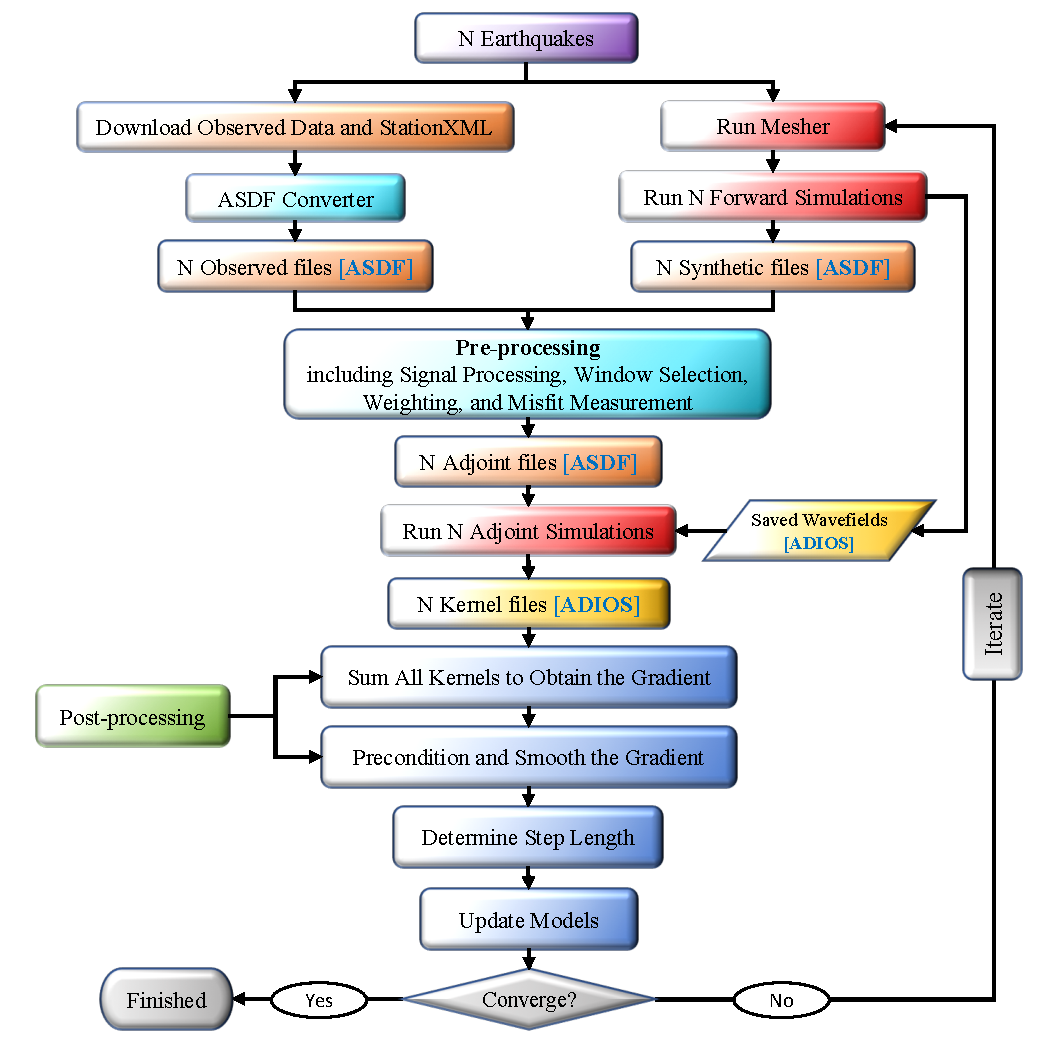
\includegraphics[width=\textwidth]{ch-GLADM25/figures/adjoint_workflow_6.pdf}
  \caption[Adjoint tomography workflow]{\small{Adjoint tomography workflow.}}
  \label{fig:adjoint_workflow}
\end{figure}

\subsection{Forward simulations}

The observed seismograms need to be compared to corresponding synthetic seismograms
for the purpose of making measurements.
The forward simulations are based on the global spectral-element solver
SPECFEM3D\_GLOBE~\cite{KoTr02a,KoTr02a}, and take a CMT solution, a relevant list
of stations, and the current earth model as input.
The solver is GPU accelerated, and the simulations are performed on the Cray supercomputer ``Titan''
at the OLCF.
To simulate 120-min seismograms with a shortest period of 17~s on 384 NVIDIA
Tesla K20X GPUs takes approximately 10~min of wall clock time.

The calculation of Fr\'echet derivatives requires
access to snapshots of the forward wavefield as part of the parsimonious storage
algorithm developed by~\cite{KoXiBoPeSaLiTr16},
with rapid I/O facilitated by ADIOS~\cite{liu2014hello}.
For the current simulation setup,
this requires about 1~TB of storage per earthquake,
so for 1,480 earthquakes this adds up to 1.5~PB.
This volume of data is generated during~$\sim$6~hours of simulations.
Based on our experience, ADIOS is capable of achieving~$\sim$120~GB/s
of sustained I/O on OLCF resources.
Given that typical write speeds for modern hard disks are~$\sim$100~MB/s,
it would be extremely difficult to carry out global adjoint tomography without the ADIOS library.

\subsection{Seismic data processing}

%\begin{figure}
%  \centering
%  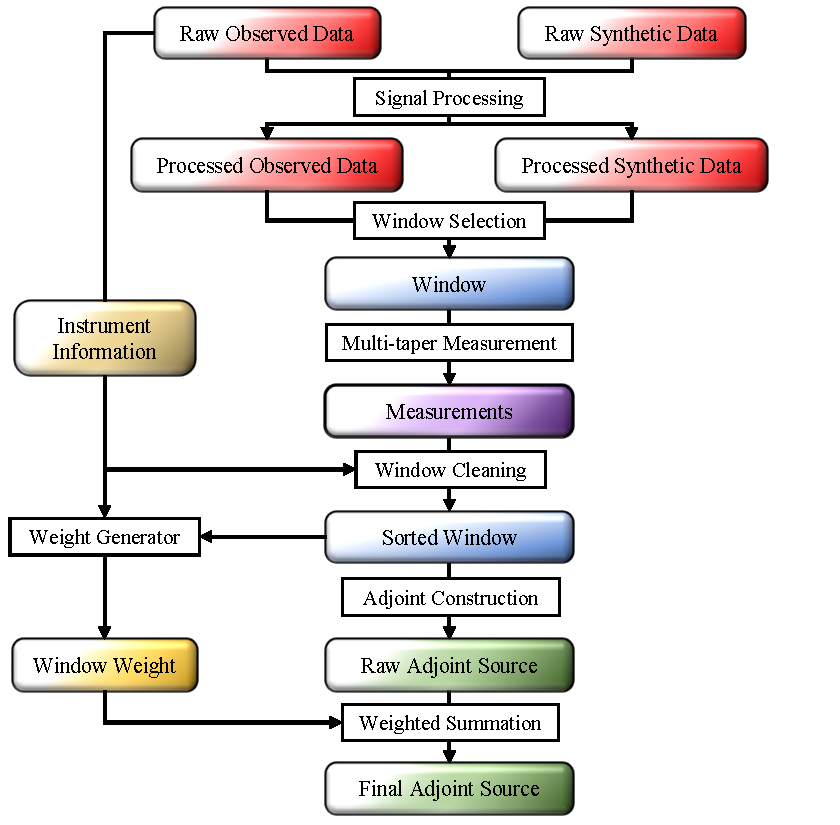
\includegraphics[width=0.8\textwidth]{ch-GLADM25/figures/Preprocess_workflow.pdf}
%  \caption[Sub-workflow workflow for preprocessing seismic data]
%  {\small{Sub-workflow workflow for preprocessing seismic data.}}
%  \label{fig:preprocess_workflow}
%\end{figure}

The seismic data preprocessing workflow takes raw observed and synthetic data as input,
and generates adjoint sources for data assimilation as output.
From a computational perspective, the preprocessing workflow consumes only~1\%
of the overall computational requirements.
But from the perspective of the tomographic inversion, this is by far the most
important stage of the adjoint tomography workflow,
directly and fundamentally impacting the outcome.
Any ``bad data'' assimilated at this stage may contaminate the gradient and
ultimately the final model.

We use millions of seismograms generating tens of millions of measurement windows,
making data selection through human interaction impossible.
The preprocessing workflow automates this task,
most importantly via the time window selection tool FLEXWIN~\cite{maggi2009automated}.
Every seismogram and potential measurement goes through multiple checks and and
balances before acceptance or rejection.

\begin{figure}
  \centering
  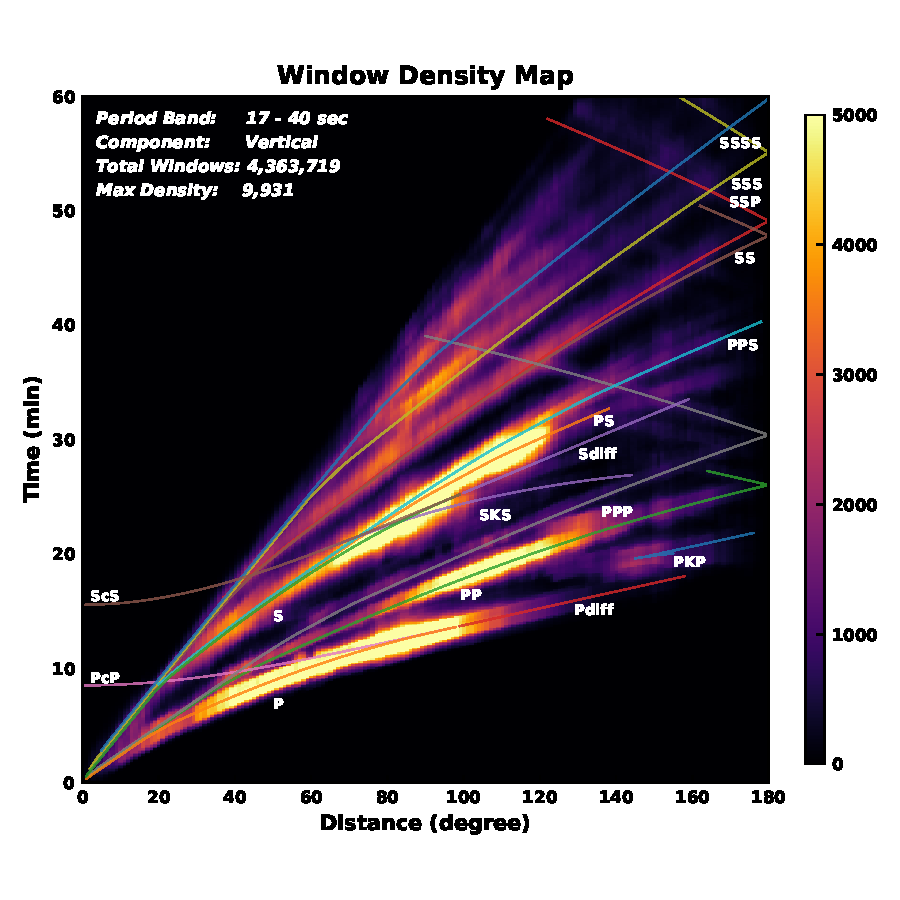
\includegraphics[width=0.9\textwidth]{ch-GLADM25/figures/window_colorbar_linear_Z.pdf}
  \caption[Time-distance plot for vertical component 17--40~s body waves]
  {\small{Time-distance plot for vertical component 17--40~s body waves showing a measurement window density map.
  A total of 4,363,719 time windows were discretized into 1~degree epicentral distance and 1~s time bins.
  The maximum window count is 9,931 in the 85--86$^\circ$ distance and 1,375--1,376~sec time bin.
  Major traveltime branches are labeled. Note that the plot contains data from events with a wide variety of depths, so the branches are for identification purposes only.
  }}
  \label{fig:window_density_Z}
\end{figure}

As illustrated in Fig.~\ref{fig:preprocess_workflow}, the preprocessing workflow
includes the following phases.
\begin{enumerate}
  \item Signal processing to remove the instrument response from observed data
    to recover ground displacement using ObsPy~\cite{obspy2010}. Both observed and synthetic data are bandpass
    filtered, and the horizontal components are rotated to obtain the radial and transverse components of motion.
  \item Window selection on a pair of
    observed and synthetic seismograms. PyFLEX (a Python version
    of FLEXWIN by \cite{krischer2015}) is
    used to automatically generate windows where observed and
    synthetic data are sufficiently close to make measurements based on user defined
    criteria.
  \item Cross-correlation traveltime or multi-taper phase measurements in selected windows.
  \item Window sorting and cleaning based on statistical analyses of all measurements to eliminate outliers.
  \item Preliminary adjoint source construction based on the sorted windows.
  \item Calculation and assignment of weights, as discussed in Section~\ref{section:misfit}.
  \item Construction of the final, properly weighted, adjoint sources.
\end{enumerate}

To illustrate which seismic phases end up being picked,
Figs.~\ref{fig:window_density_Z}, \ref{fig:window_density_R}, and \ref{fig:window_density_T} show time-distance plots
for vertical, radial, and transverse component 17--40~s body waves,
respectively,
in which the PyFLEX window count is used to identify parts of seismograms being assimilated.
The figures nicely highlight all the well-known body traveltime branches.
Collectively, the numerous compressional-wave arrivals identified in Figs.~\ref{fig:window_density_Z} and~\ref{fig:window_density_R} are of great importance, because they help constrain the compressional wavespeed structure in the model.
The PyFLEX window selection algorithm is currently configured not to pick body waves after the arrival of the surface waves, which is why the PcP and ScS branches are missing at shorter epicentral distances.
This is something we will reconsider in future applications, perhaps by introducing aspects of machine learning. 

\begin{figure}
  \centering
  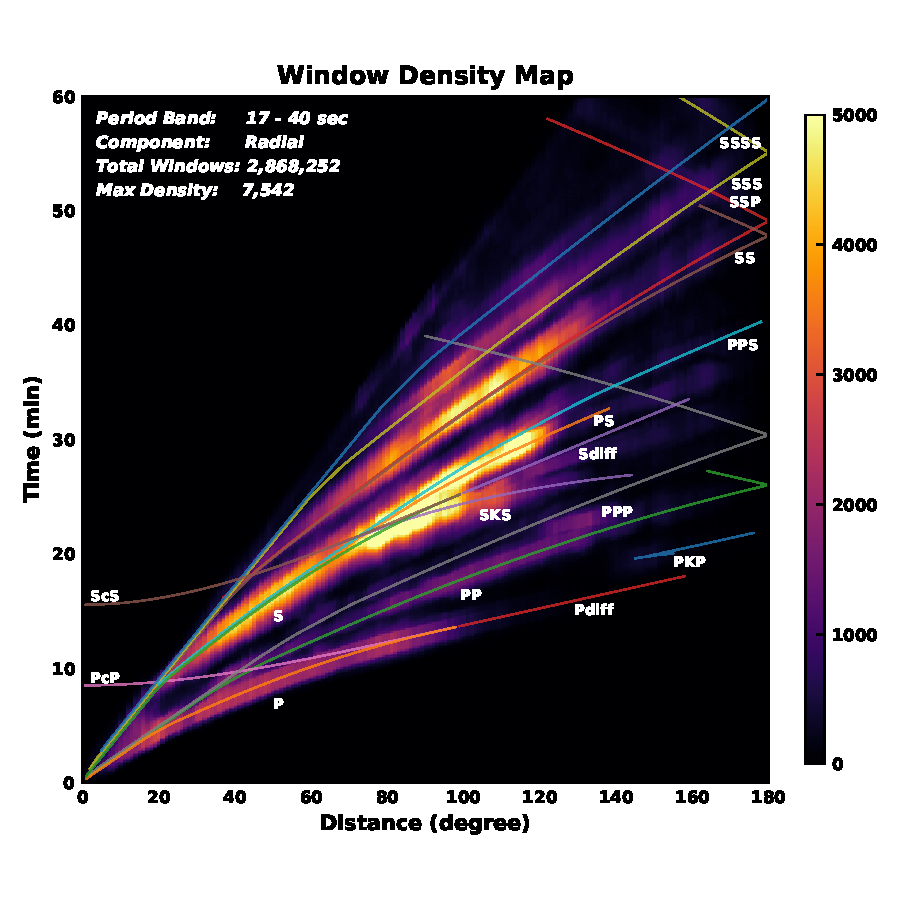
\includegraphics[width=0.9\textwidth]{ch-GLADM25/figures/window_colorbar_linear_R.pdf}
  \caption[Time-distance plot for radial component 17--40~s body waves]
  {\small{Same as Fig.~\ref{fig:window_density_Z}, except for radial component 17--40~s body waves.
   A total of 2,868,252 time windows were discretized into 1~degree epicentral distance and 1~s time bins.
  The maximum window count is 7,542 in the 86--87$^\circ$ distance and 1,378--1,379~s time bin.
   }}
  \label{fig:window_density_R}
\end{figure}

\begin{figure}
  \centering
  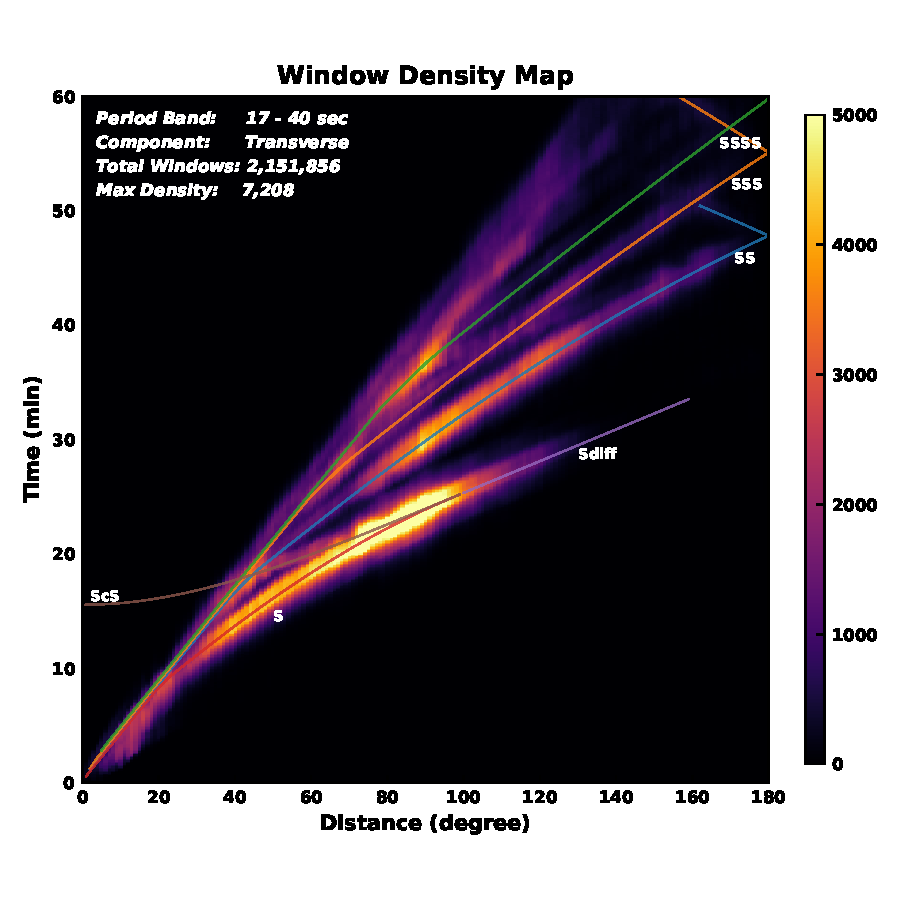
\includegraphics[width=0.9\textwidth]{ch-GLADM25/figures/window_colorbar_linear_T.pdf}
  \caption[Time-distance plot for transverse component 17--40~s body waves]
  {\small{Same as Fig.~\ref{fig:window_density_Z}, except for transverse component 17--40~s body waves.
   A total of 2,151,856 time windows were discretized into 1~degree epicentral distance and 1~s time bins.
   The maximum window count is 7,208 in the 89--90$^\circ$ distance and 1,398--1,399~s time bin.
   Only SH traveltime branches are labeled.}}
  \label{fig:window_density_T}
\end{figure}

\subsection{Adjoint Simulations}

Collectively,
the adjoint simulations are the most expensive stage of the workflow. 
Adjoint simulations take the adjoint sources as input, and generate Fr\'echet
derivatives of the four model parameters as output.
The computational cost of one adjoint simulation is roughly twice ($\sim25$~min) that of
a forward simulation, since the forward wavefield is recalculated for convolution with
the adjoint wavefield during the adjoint simulation.
Using this procedure,
both the forward and adjoint wavefield are calculated in forward time,
and attenuation is accurately taken into account in both simulations.

\subsection{Postprocessing}

The postprocessing stage of the workflow takes Fr\'echet derivatives as input and
generates a model update as output.
It involves the follow steps.
\begin{enumerate}
  \item Summation of the individual Fr\'echet derivatives for each earthquake to obtain the overall gradient of the misfit function. The contribution of each source is weighted to balance
    the uneven distribution of earthquakes based on the weighting strategy discussed in Section~\ref{section:misfit} .
  \item Smoothing of the raw misfit gradient using a 3D Gaussian, which
    serves as a regularization procedure. Instead of using a changing
    smoothing radius based upon the ``ray density''~\cite{bozdaug2016global},
    we used a fixed value at a given iteration, following~\cite{zhu2012structure}.
  \item Preconditioning of the smoothed gradient based on a technique proposed by~\cite{luo2013strategies}.
  \item Line search to determine the magnitude of the model update.
  The search direction is determined using a nonlinear conjugate gradient method~\cite{wright1999numerical} (iterations 16--21) or a Limited-memory Broyden\-Fletcher\-Goldfarb\-Shanno (L-BFGS) quasi-Newton method (iterations 22--25).
  We used a subset of 160 earthquakes to conduct the line search and determine the step length.
\end{enumerate}

\subsection{Workflow management}

There are more than ten stages in the adjoint tomography workflow,
and each stage involves thousands of small tasks.
For every model iteration,
we performed up to 1,480 forward and adjoint simulations, each involving hundreds of
compute cores and graphics cards, as well as heavy I/O.
The workflow is prone to human error and hardware failure, making it fragile~~\cite{Lefebvre2018}.
For these reasons, we hardened the workflow by taking advantage of modern
workflow management software.
We selected EnTK as our
workflow management engine~\cite{EnTK2017}, and developed complementary seismic tomography
workflow tools.
The workflow engine can automatically detected job failures both from the
HPC system and via user-defined functions. This enables us to keep track of
all tasks and semi-automatically resubmit jobs if necessary.
Given that most HPC system time is spent waiting in the job queue, automatic
failure detection and relaunching greatly shortens the overall time to solution.

\section{Misfit evolution}
\label{section:misfit_evolution}

The inversion went through ten iterations in a number of stages, as documented
in this section. The evolution of the overall misfit function~(\ref{eq:misfit1})
as well as its behavior in the various measurement categories is summarized
in Fig.~\ref{fig:misfit}.

\begin{figure}
  \centering
  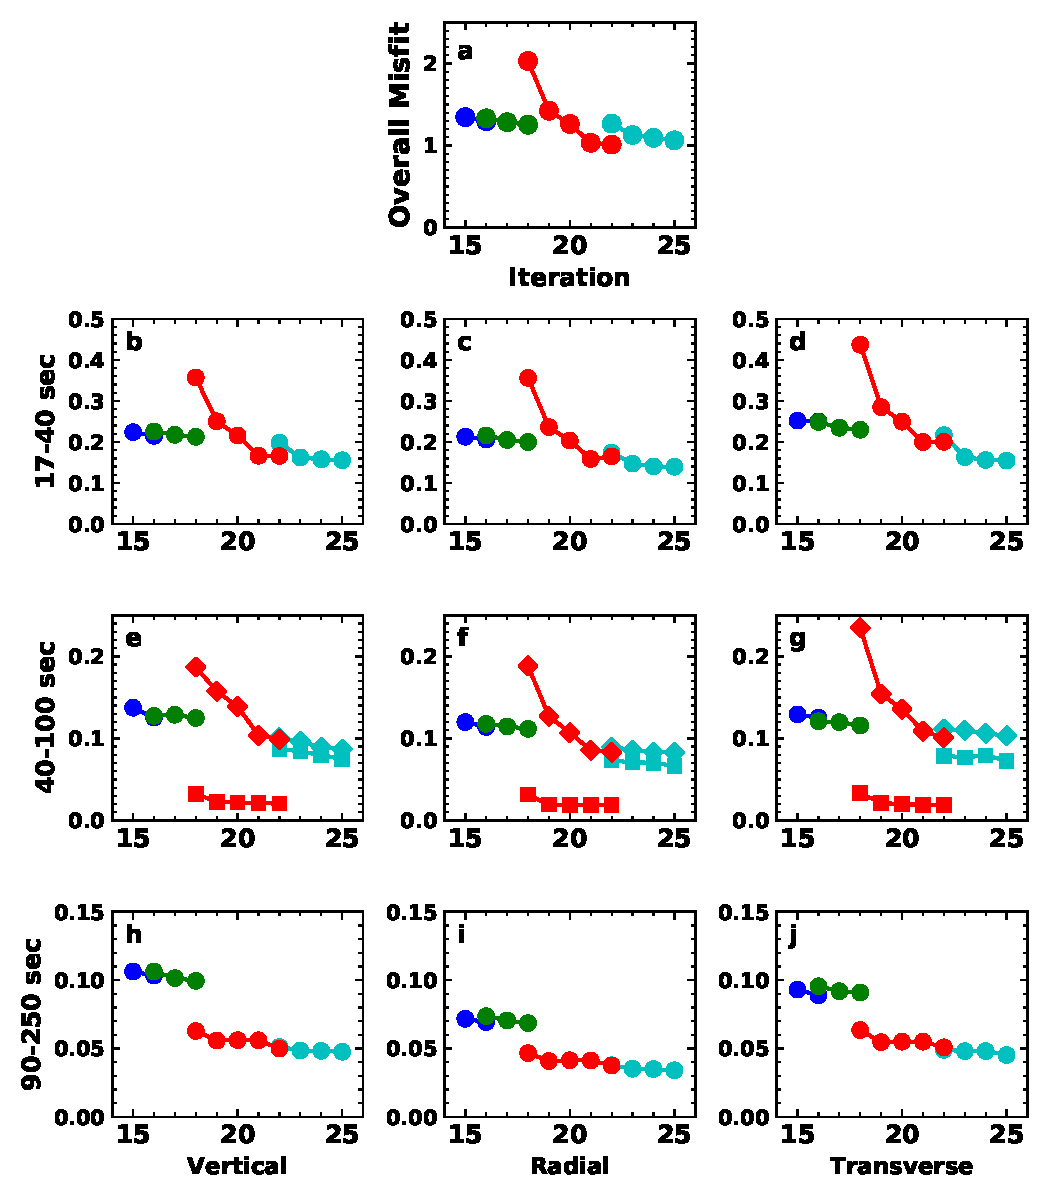
\includegraphics[width=0.8\textwidth]{ch-GLADM25/figures/misfit.pdf}
  \caption[Evolution of misfit function from GLAD-M15 to GLAD-M25]
  {\small{Evolution of the misfit function from GLAD-M15 to GLAD-M25.
  Each color denotes different stages of the inversion, as discussed in Sections~\ref{sec:I}--\ref{sec:III}.
  (a) Evolution of the total misfit. (b)--(j) Misfit in
  each period band (rows) on three components (columns). (e)--(g) Since iteration 18,
  we  split the 40--100~s period band into two
  measurement categories: body waves (diamonds) and surface waves
  (squares).
  }}
  \label{fig:misfit}
\end{figure}

\subsection{Stage~I: Iterations 15--17}
\label{sec:I}

Starting model GLAD-M15 was constructed using a database of 253 earthquakes.
For iterations 15--17 of the inversion we used an expanded database of 520 events.
Our focus was to validate and test our software and workflow before scaling up
to a larger database of 1,040 events.
For these iterations we used three period bands, namely,
17--40~s, 40--100~s, and 90--250~s,
and we used a nonlinear conjugate
gradient method to update the model.

\subsection{Stage~II: Iterations 18--21}

We see an abrupt change in the value of the misfit function at iteration~18
in Fig.~\ref{fig:misfit},
reflecting the addition of 520~events to the inversion database,
and a change in the weighting strategy for 40--100~s surface waves.
For iterations 18--21 we split the 40--100~s period band into two, separating the
body and surface waves (Figs.~\ref{fig:misfit}e--g).
Since body and surface waves sample different parts of the mantle,
this split facilitated more control over the spatial distribution of the model update.
Because the 17th iteration model explains 40--100~s surface wave data relatively well,
we reduced their weight on all three components for iterations 18--21,
as indicated by the lower red curves in Figs.~\ref{fig:misfit}e--g.

The misfit reduction for 17--40~s body waves (Figs.~\ref{fig:misfit}b--d) tapers off by
iteration~21, prompting us to add more earthquakes and change the weighting strategy again by reintroducing 40--100~s surface waves.

% Table~\ref{table:measurement_category} shows the four passbands we used in Stage~II, tabulating misfit reductions in all four passbands on three components,
% that is, in twelve measurement categories.

% \begin{table}[!htb]
%   \centering
%   \begin{tabular}{|c|c|c|c|}
%     \hline
%     ~          &  Vertical & Radial &  Transverse \\
%     \hline
%     17--40~s   &   P-SV          & P-SV           & SH   \\
%     40--100~s  &   P-SV          & P-SV            & SH \\
%     40--100~s  &   Rayleigh   & Rayleigh    & Love \\
%     90--250~s  &   All                 & All                  & All  \\
%     \hline
%   \end{tabular}\\
%   \caption{\small{Twelve measurement categories used for iterations 18--25.
%   Before iteration~18, the 40--100~s body and surface waves categories were combined into a single category on each component, resulting in nine categories.}}
%   \label{table:measurement_category}
% \end{table}

\subsection{Stage~III: Iterations 22--25}
\label{sec:III}

At iteration~22 we added another 440 earthquakes to the database,
bringing the total to 1,480 events,
and we changed the 40--100~s surface wave weights back to their
setting in Stage~I. During this stage we switched from a nonlinear
conjugate gradient optimization algorithm to an L-BFGS quasi-Newton method.

\subsection{Misfit assessment}
\label{section:Misfit assessment}

In the previous sections we discussed the evolution of the misfit through
three key stages of the inversion.
It is important to note that ``the misfit function'' is, in fact, a
continually moving target, because at every iteration the number of
measurements increases as the model improves,
and the number of earthquakes increases at iterations~18 and~22.

In this section we calculate specific changes in misfit using all 1,480
earthquakes and an identical set of weights and windows for three models,
namely, GLAD-M25, GLAD-M15, and S362ANI combined with CRUST2.0.
Table~\ref{table:misfit_reduction_M15_M25} summarizes the changes in fit in
the twelve measurement categories between the new model, GLAD-M25, and its
starting model, GLAD-M15, and between GLAD-M25 and model S362ANI combined
with CRUST2.0, which was the starting model for the GLAD-M15 inversion.

In all categories we observe significant misfit reductions,
with dispersive 40--100~s surface waves exhibiting the largest improvements.
The improvements in fit per component are comparable in all period bands,
indicating that the various categories are reasonably well balanced in the
assessment of misfit.

\begin{table}
  \centering
  \begin{tabular}{|c|c|c|c|}
    \hline
    ~          &  Vertical (\%) & Radial (\%) &  Transverse (\%) \\
    \hline
    %17--40~s  body waves    &   17.4 (31.1)   &       21.1 (37.1) &       24.6 (42.2) \\
    %40--100~s body waves    &   16.8 (31.3)  &       21.3 (40.2)  &       21.7 (42.0) \\
    %40--100~s surface waves &   28.5 (50.1)  &       28.3 (51.1) &       28.4 (53.8)  \\
    %90--250~s surface waves &   14.5 (36.2)  &       13.4 (38.8) &       25.7 (38.6) \\
    17--40~s  body waves    &   19.1 (37.3)   &       23.7 (46.3) &       28.2 (54.8) \\
    40--100~s body waves    &   18.3 (37.5)   &       24.0 (51.4) &       24.5 (54.5) \\
    40--100~s surface waves &   33.6 (69.6)   &       33.3 (71.5) &       33.5 (77.2) \\
    90--250~s all waves &   15.7 (44.9)   &       14.4 (49.1) &       29.6 (48.7) \\
    \hline
  \end{tabular}\\
  \caption[Changes in fit for 1,480 earthquakes used as inversion dataset]
  {\small{Changes in fit in the twelve measurement categories
    between the new model, GLAD-M25, and its starting model, GLAD-M15,
    and, in parentheses, between GLAD-M25 and model S362ANI combined with
    CRUST2.0, which was the starting model for the GLAD-M15 inversion.}}
  \label{table:misfit_reduction_M15_M25}
\end{table}

% \begin{table}[!htb]
%   \centering
%   \begin{tabular}{|c|c|c|c|}
%     \hline
%      ~          &  Vertical(\%) & Radial(\%) &  Transverse(\%) \\
%     \hline
%     17--40s body waves     &    31.1    &       37.1 &       42.2 \\
%     40--100s body waves    &    31.3    &       40.2 &       42.0 \\
%     40--100s surface waves &    50.1    &       51.1 &       53.8 \\
%     90--250s               &    36.2    &       38.8 &       38.6 \\
%     \hline
%   \end{tabular}\\
%   \caption{\small{Misfit Reduction from M00 to M25 for 1480 earthquakes used in the inversion.}}
%   \label{table:misfit_reduction_M00_M25}
% \end{table}

\subsection{Histogram comparisons}
\label{section:Histogram comparisons}

Another way to evaluate model performance is by assessing the distribution
of measurements in the various categories.
Again we use all 1,480 events and a set of identical windows on all three components
to assess GLAD-M25, GLAD-M15, and S362ANI combined with CRUST2.0.
The total number of selected windows,
determined using model GLAD-M25, exceeds 18~million.
Fig.~\ref{fig:phase_hist} shows histograms of the resulting phase
measurements in all twelve measurement categories.
We observe that the distributions generally become better centered on zero,
and that all standard deviations are steadily reduced.
Again we note that the inversion is aimed at reducing the overall misfit,
so there are small trade-offs between different measurement categories.

\begin{figure}
  \centering
  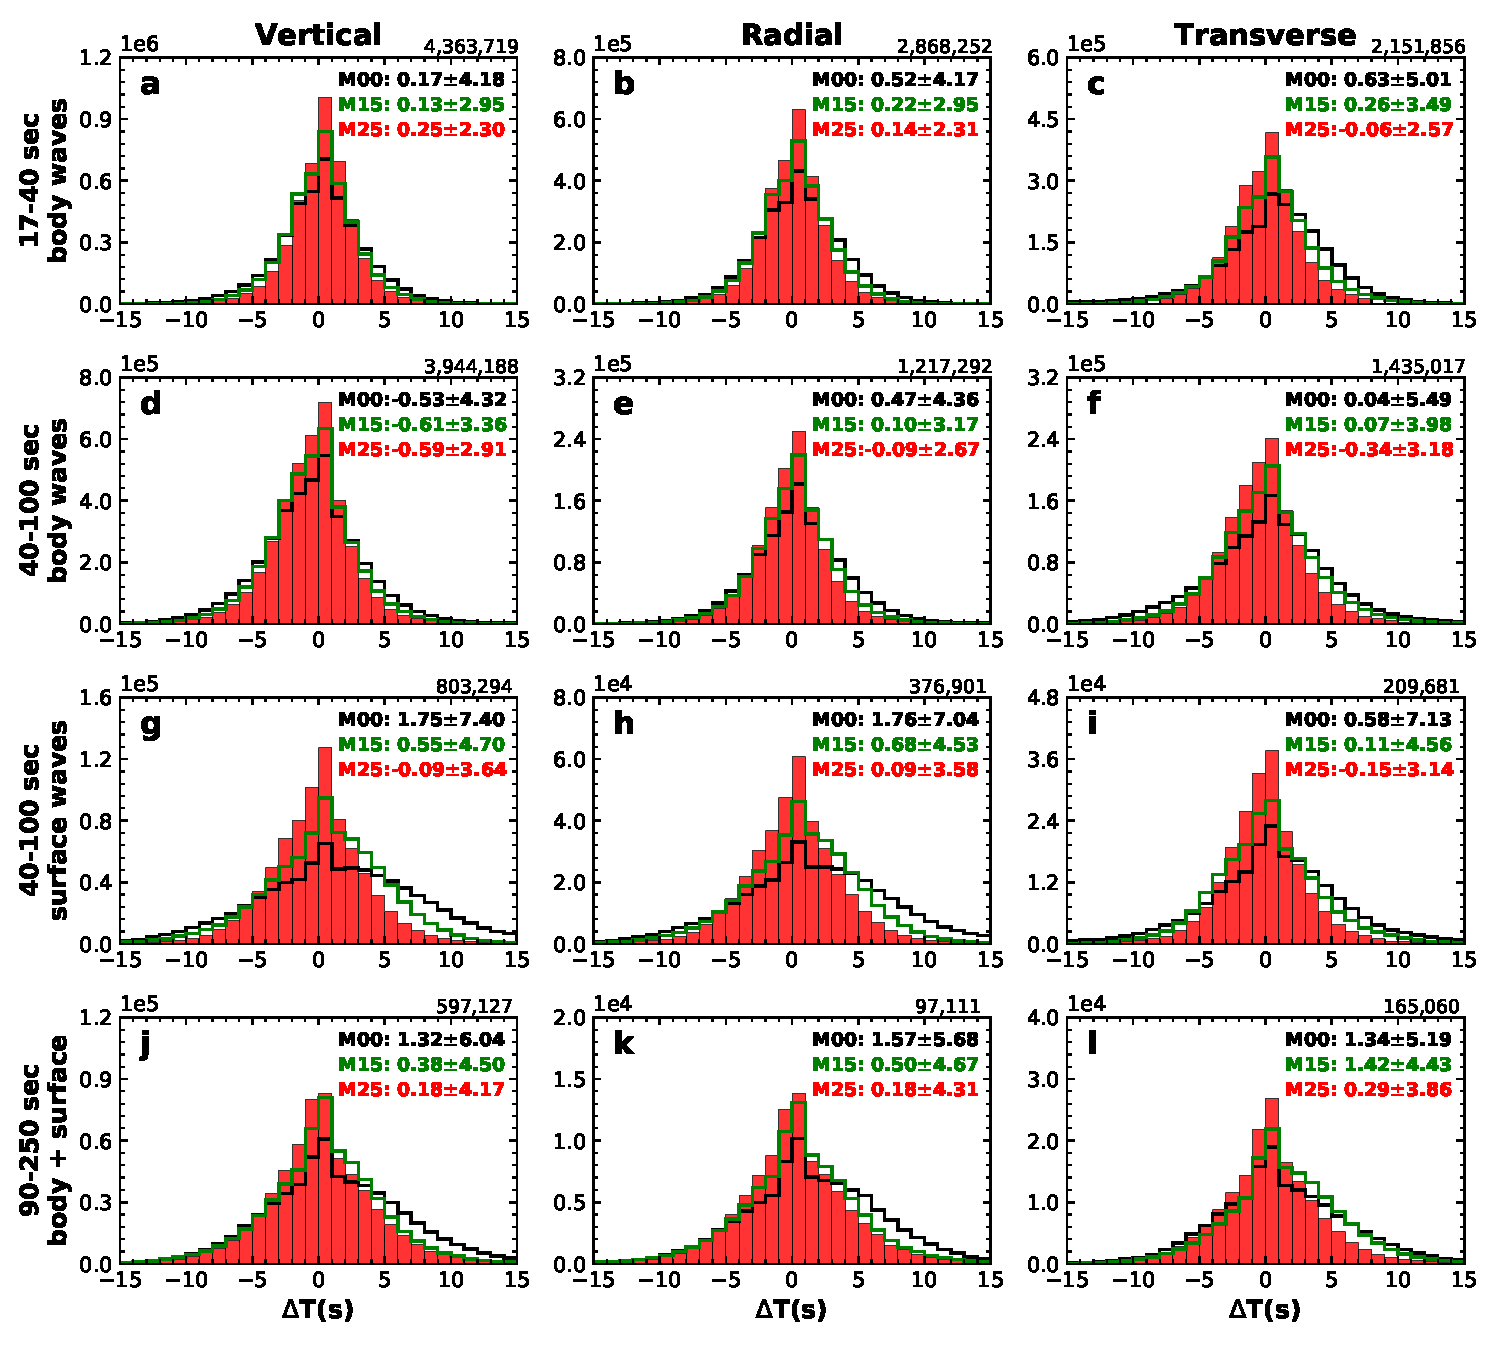
\includegraphics[width=\textwidth]{ch-GLADM25/figures/dt_histogram.pdf}
  \caption[Histograms of phase measurements in all twelve measurement categories]
  {\small{Histograms of phase measurements in all twelve measurement categories for S362ANI combined with CRUST2.0 (M00, Black), GLAD-M15 (M15, Green), and GLAD-M25 (M25, Red).
  Each column represents one component and each row corresponds to a period band.
  The numbers above the top right of each panel denote the number of measurements in the corresponding category.
  The total number of measurements is 18.2 million.
  The mean and standard deviations of the phase measurements for the three models are displayed in the top right corner of each panel.}}
  \label{fig:phase_hist}
\end{figure}

Fig.~\ref{fig:PS_phase_hist} shows histograms of 17--40~s P-wave traveltime anomalies on the vertical and radial components, and 17-40~s S-wave traveltime anomalies on the transverse component.
Both P and S waves exhibit consistent reductions in terms of both mean and variance. 

\begin{figure}
  \centering
  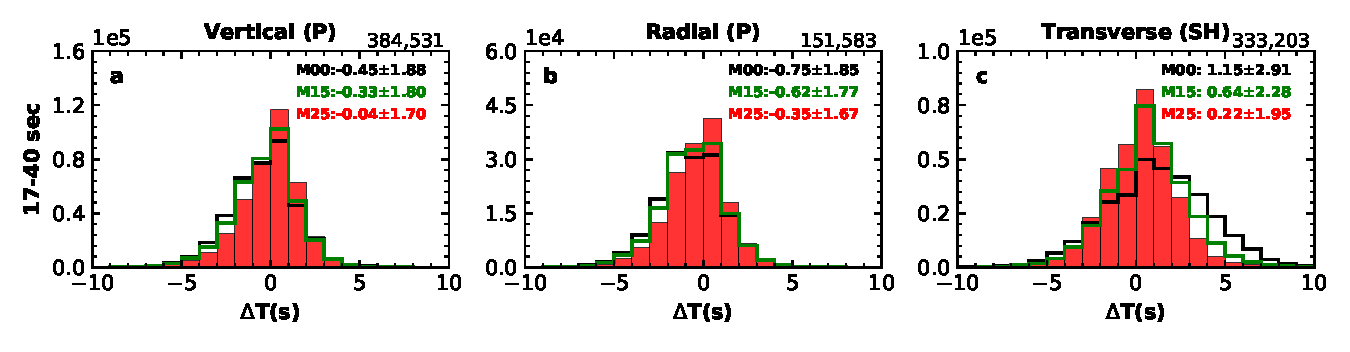
\includegraphics[width=\textwidth]{ch-GLADM25/figures/dt_histogram_phase.pdf}
  \caption[Histograms of 17--40~s traveltime anomalies of P and SH arrivals]
  {\small{Histograms of 17--40~s traveltime anomalies of P (vertical and radial), and SH (Transverse) arrivals for models S362ANI combined with CRUST2.0 (M00, Black), GLAD-M15 (M15, Green), and GLAD-M25 (M25, Red).
  }}
  \label{fig:PS_phase_hist}
\end{figure}

Fig.~\ref{fig:amp_hist} shows histograms of the amplitude
measurements for all twelve measurement categories,
which were not used in the current inversion.
Despite this,
we observe modest reductions in all standard deviations of the histograms.
The histograms are nicely centered, indicating that the moment magnitudes are
suitably selected, because the scalar moment affects all measurement categories equally.
In the next phase of our ongoing inversion we plan to begin assimilating amplitude measurements while simultaneously adding shear attenuation as a new model parameter.

\begin{figure}
  \centering
  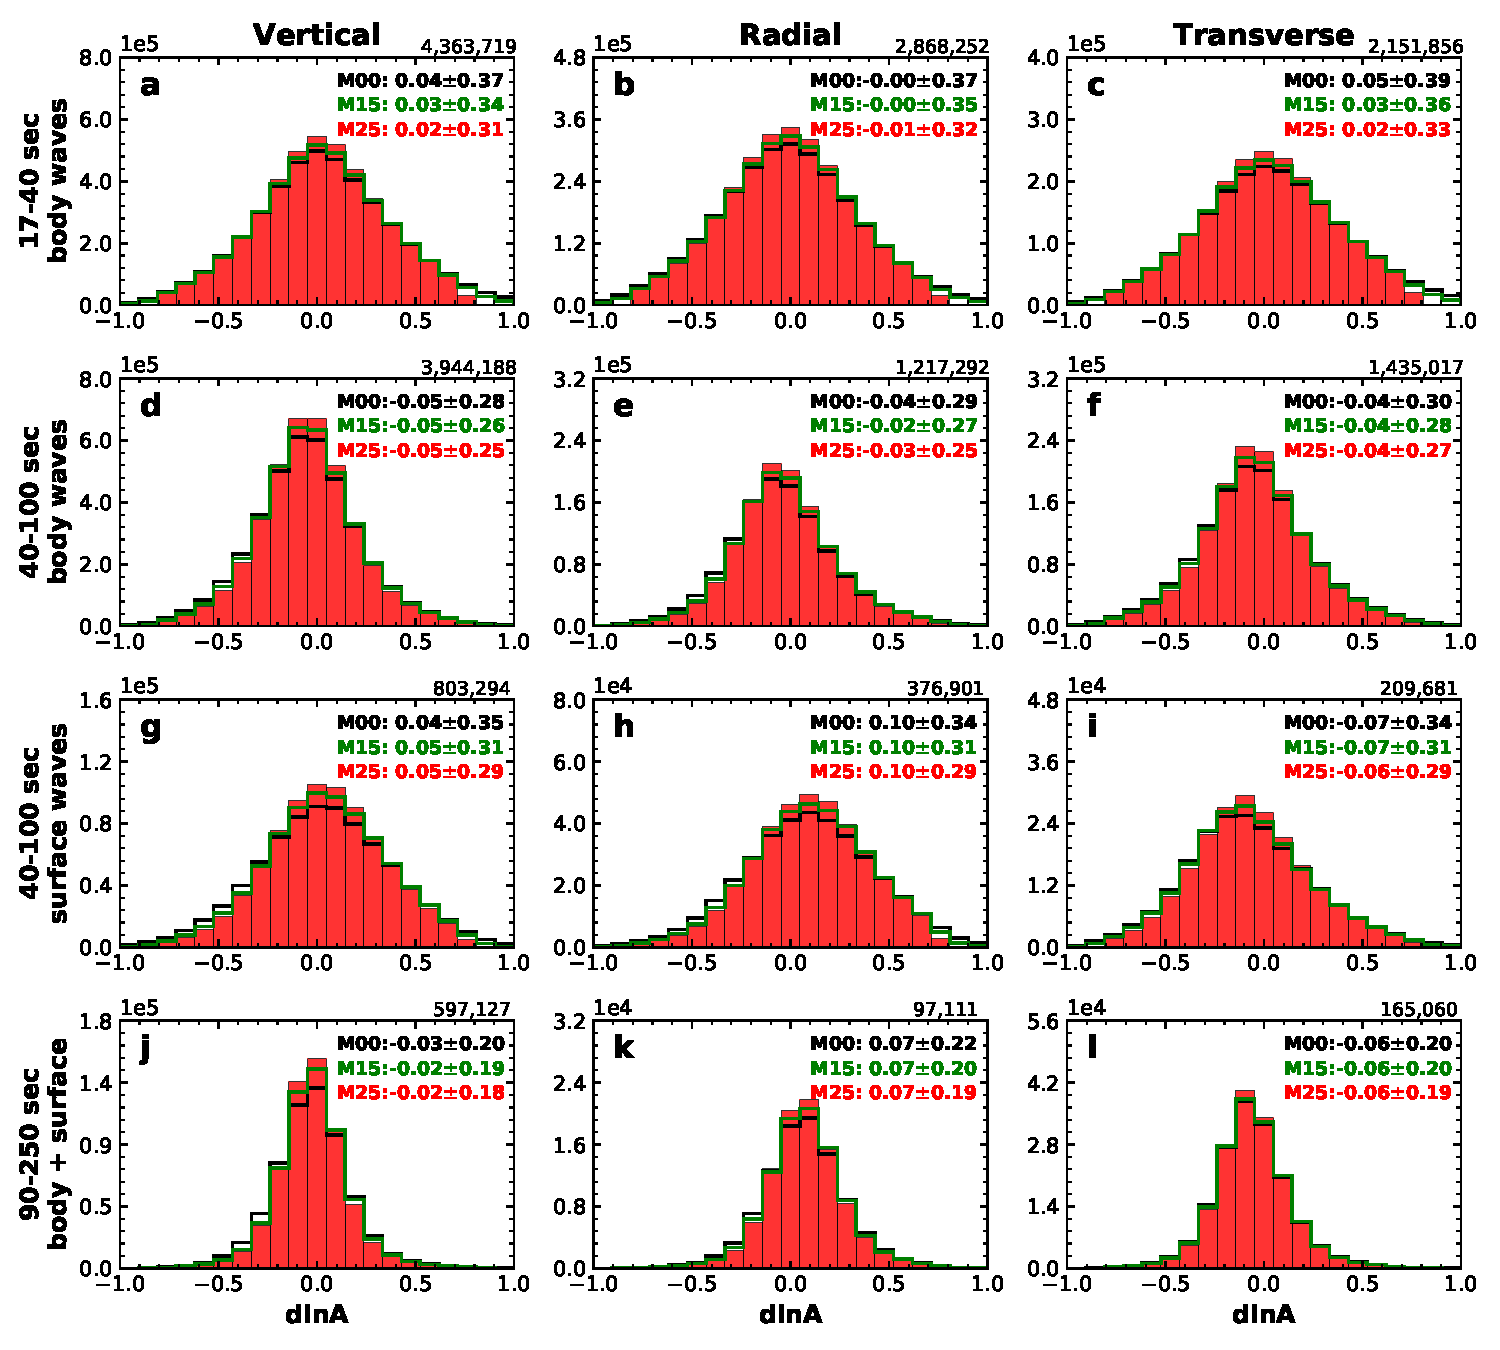
\includegraphics[width=\textwidth]{ch-GLADM25/figures/dlna_histogram.pdf}
  \caption[Histograms of amplitude measurements in all twelve measurement categories]
  {\small{Same as Fig.~\ref{fig:phase_hist} except for amplitude measurements. These measurements are currently not used in the inversion.}}
  \label{fig:amp_hist}
\end{figure}

\section{Model evaluation}
\label{section:evaluation}

% In this section we evaluate model GLAD-M25 further based on a point-spread
% function resolution analysis as well as a ``held-out'' data set, that is,
% a set of data not used in the actual structural inversion.

\subsection{Point-spread function analysis}

Checkerboard tests or tests involving a chosen known structure, e.g., a plume or slab,
are frequently used to evaluate resolution in a tomographic inversion.
Such tests are extremely expensive in FWI and adjoint tomography, because they
require roughly the same computational resources as the actual inversion.
In lieu of such tests, we previously performed two point-spread function (PSF) analyses
for model GLAD-M15~\cite{bozdaug2016global}.
Since GLAD-M25 --- like its predecessor GLAD-M15 --- uses waves with a shortest period of 17~s
but an earthquake database that is six times larger,
we can expect improved versions of these already successful PSF tests.
In the interest of focusing our efforts on obtaining the new model,
we chose to direct our limited OLCF INCITE allocation towards the actual inversion
rather than improved PSF tests.

\subsection{Held-out data set}

\begin{figure}
  \centering
  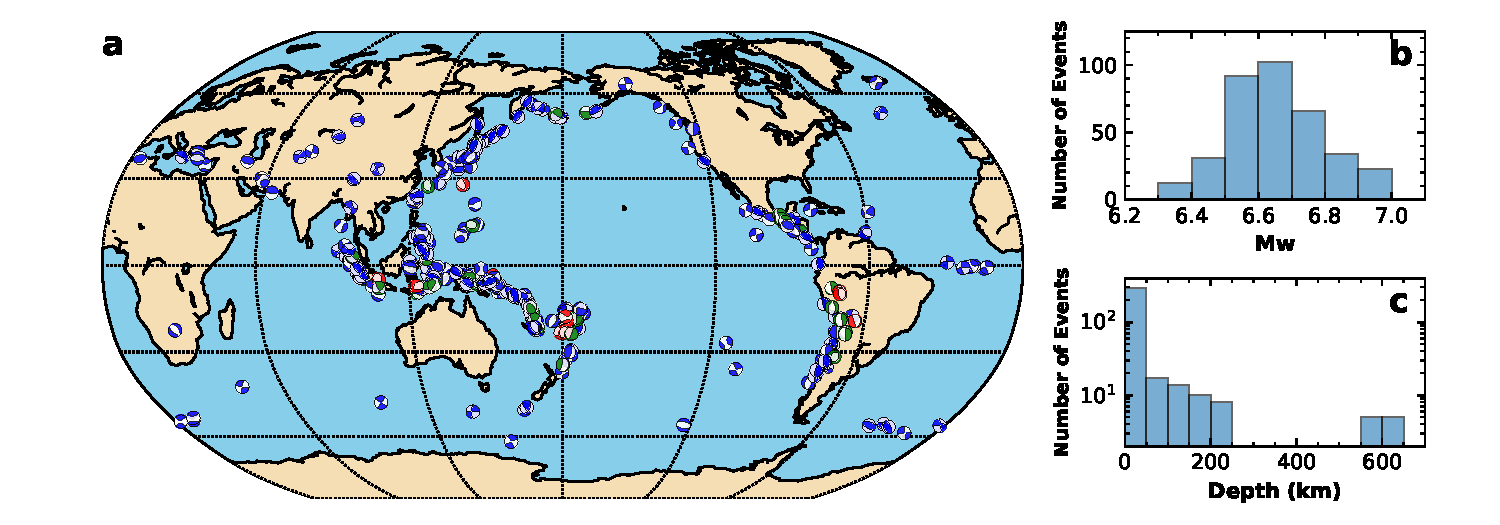
\includegraphics[width=\textwidth]{ch-GLADM25/figures/events_360.pdf}
  \caption[Distribution of 360 earthquakes used as held-out data]
  {\small{Summary of the held-out database containing 360 earthquakes. Theses events were not used in the structural inversion. (a)~Distribution of events color coded by depth range as in Fig.~\ref{fig:event_1480}. (b) \& (c)~Histograms of moment magnitude and depth.}}
  \label{fig:events_360}
\end{figure}

Following the approach of \cite{tape2009adjoint}, \cite{chen2015multiparameter},
and \cite{bozdaug2016global}, we selected 360 earthquakes that were not used
in the actual inversion. This held-out data set consists of all magnitude 6.3--7.0
earthquakes in the global CMT catalog that were not used in the inversion.
We chose larger events to generate as many measurements as possible.
We calibrated the centroid time and scalar moment using a grid search based on
3D synthetics calculated in GLAD-M25.
Fig.~\ref{fig:events_360} summarizes the properties of the held-out database.

First, we repeated the misfit assessment discussed in
Section~\ref{section:Misfit assessment} for the held-out database.
Table~\ref{table:misfit_reduction_M15_M25_360} summarizes the reductions
in misfit for the held-out database for model GLAD-M25 compared to GLAD-M15
as well a S362ANI combined with CRUST2.0.
It is a validation of our approach to see that the reductions are comparable to the
values tabulated in Table~\ref{table:misfit_reduction_M15_M25} for the actual inversion.
Overall, the reductions are slightly smaller, partly due to the fact that we did not
conduct full CMT inversions for the held-out database.

\begin{table}
  \centering
  %\label{tab:category}
  \begin{tabular}{|c|c|c|c|}
  \hline
  ~          &  Vertical (\%) & Radial (\%) &  Transverse (\%) \\
  \hline
  17--40~s                &          11.8 (29.2) &       14.1 (33.7) &       21.5 (43.4) \\
  40--100~s body waves    &          14.5 (26.2) &       12.9 (32.2)  &       16.9 (39.0) \\
  40--100~s surface waves &          29.3 (49.1) &       28.1 (49.4) &       23.7 (51.2) \\
  90--250~s               &          10.9 (30.9) &       14.3 (34.8)  &       24.0 (34.9) \\
  \hline
  \end{tabular}\\
  \caption[Changes in fit for 360 earthquakes used as held-out dataset]
  {\small{Changes in fit for 360 earthquakes not used in the inversion in the
      twelve measurement categories between the new model, GLAD-M25, and its
      starting model, GLAD-M15, and, in parentheses, between GLAD-M25 and model
      S362ANI combined with CRUST2.0, which was the starting model for the GLAD-M15 inversion.}}
  \label{table:misfit_reduction_M15_M25_360}
\end{table}

% \begin{table}[!htb]
%   \centering
%   %\label{tag:misfit_reduction_M00_M25_360}
%   \begin{tabular}{|c|c|c|c|}
%     \hline
%     ~          &  Vertical(\%) & Radial(\%) &  Transverse(\%) \\
%     \hline
%     17--40s                &         29.2 &       33.7 &       43.4 \\
%     40--100s body waves    &         26.2 &       32.2 &       39.0 \\
%     40--100s surface waves &         49.1 &       49.4 &       51.2 \\
%     90--250s               &         30.9 &       34.8 &       34.9 \\
%     \hline
%   \end{tabular}\\
%   \caption{\small{Misfit Reduction from M00 to M25 for 360 earthquakes as held-out data set.}}
%   \label{table:misfit_reduction_M00_M25_360}
% \end{table}

\begin{figure}
  \centering
  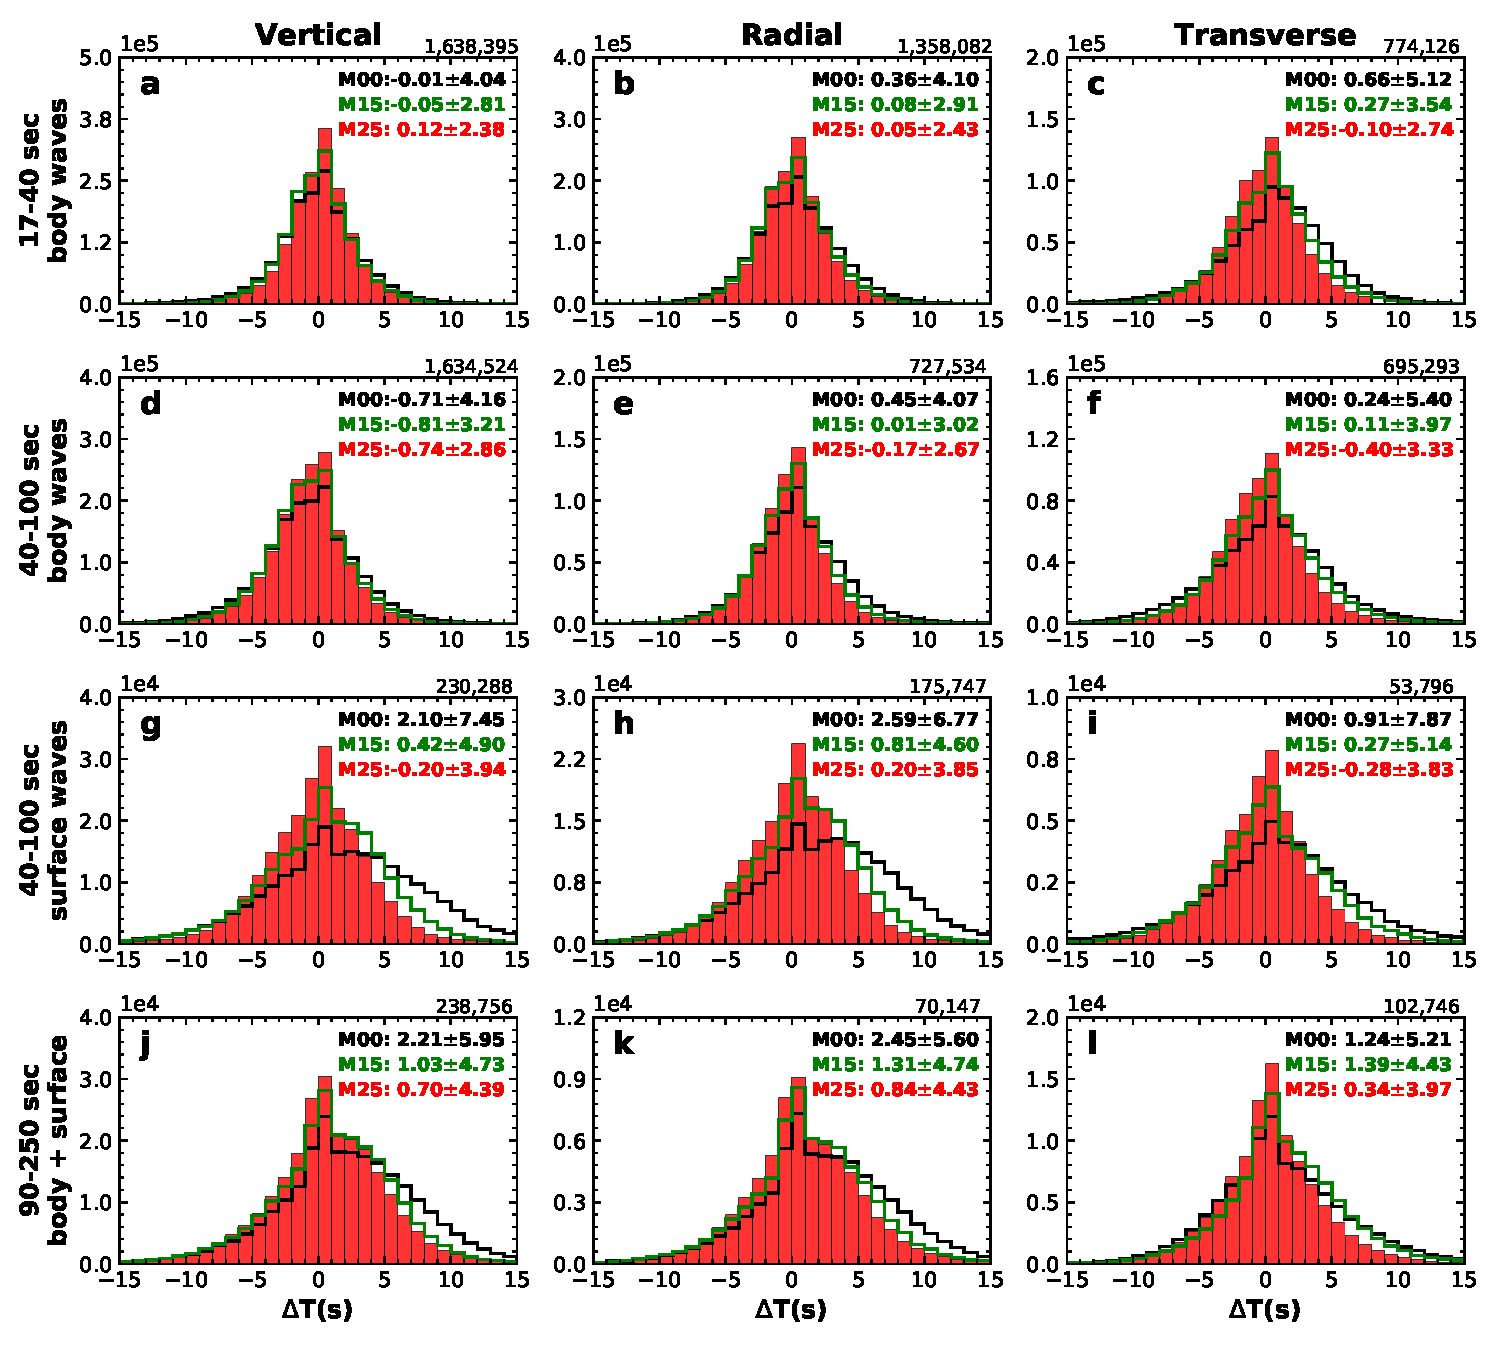
\includegraphics[width=\textwidth]{ch-GLADM25/figures/dt_histogram_360.pdf}
  \caption[Histograms of amplitude measurements in all twelve measurement categories for held-out database]
  {\small{Same as Fig.~\ref{fig:phase_hist}, except for the held-out database.}}
  \label{fig:phase_hist_360}
\end{figure}

\begin{figure}
  \centering
  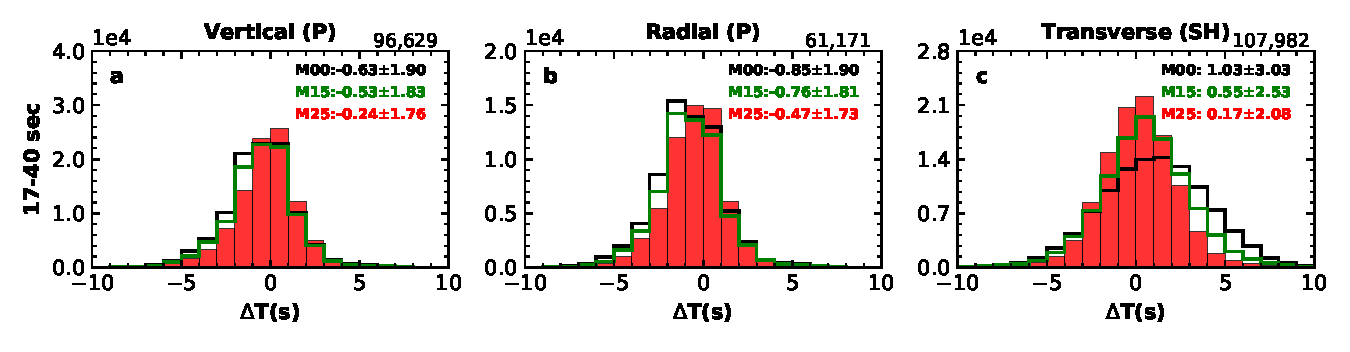
\includegraphics[width=\textwidth]{ch-GLADM25/figures/dt_histogram_360_phase.pdf}
  \caption[Histograms of 17--40~s traveltime anomalies of P and SH arrivals for held-out database]
  {\small{Same as Fig.~\ref{fig:PS_phase_hist}, except for the held-out database.}}
  \label{fig:phase_hist_360_P}
\end{figure}

Second, we repeated the histogram comparisons discussed in
Section~\ref{section:Histogram comparisons} for the held-out database.
We used a set of identical windows on all three components to assess
phase anomalies in models GLAD-M25, GLAD-M15, and S362ANI combined with CRUST2.0.
Fig.~\ref{fig:phase_hist_360} shows histograms of the resulting phase
measurements in all twelve measurement categories.
The total number of measurements exceeds 7.8~million.
As in the actual inversion,
we observe systematic decreases in all standard deviations in all twelve categories,
and we note a sharpening of the distributions centered around zero.

Finally,
direct P and S traveltime anomaly measurements were extracted and compared for three models in Fig.~\ref{fig:phase_hist_360_P}.
Again the histograms are consistent with the actual inversion,
as expected.


\section{Model GLAD-M25}
\label{section:model}

In this section we discuss model GLAD-M25 in some detail.
We begin with a global overview of the model, before concentrating on
specific geographical regions.
We conclude by highlighting various slabs and plumes.
The focus is on isotropic shear and compressional wavespeed variations.
We provide comparisons with numerous other global and regional tomographic models,
but we refrain from detailed tectonic/geodynamic interpretations,
which will be the subject of more targeted future investigations.
Our goal in the article is to discuss the construction of model GLAD-M25,
and to place it into a broader tomographic context. 

Vertical cross sections are plotted relative to the spherical average of GLAD-M25,
as discussed in Appendix~\ref{chapter:1Dmodel}.
For plotting purposes and use in other applications,
an expansion of the model in spherical harmonics and radial B-splines is
discussed in Appendix~\ref{chapter:shanalysis}.

\subsection{Global structure}

\begin{figure}
  \centering
  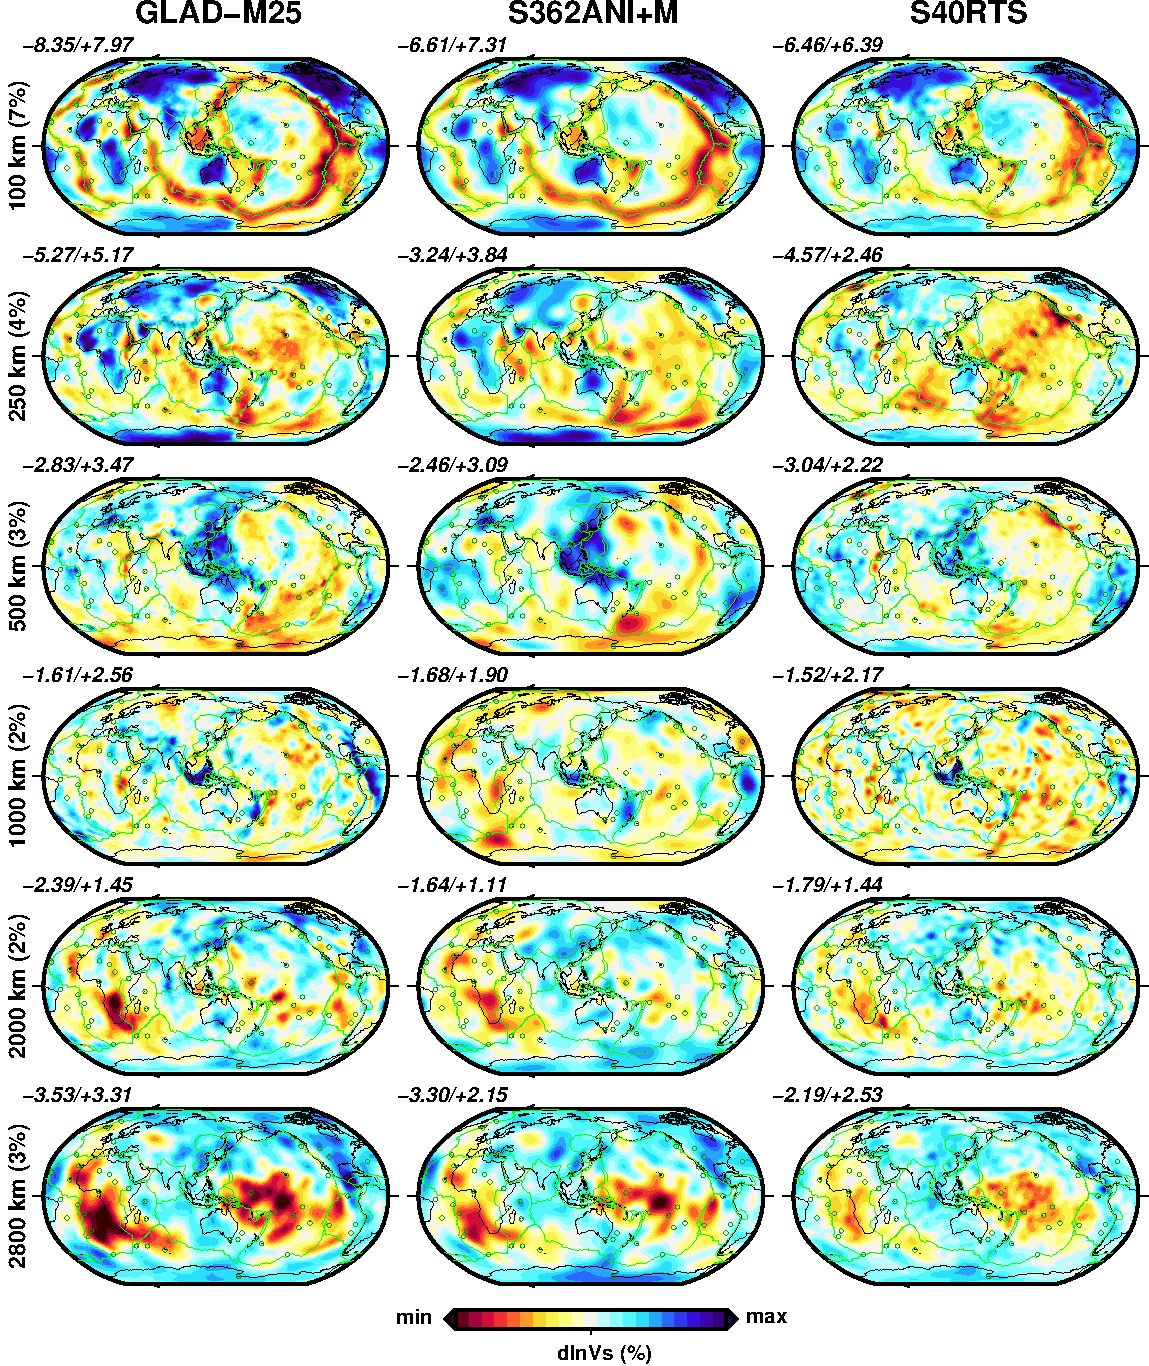
\includegraphics[width=0.9\textwidth]{ch-GLADM25/figures/depth_slice/globe_vs.pdf}
  \caption[Map views of global shear wavespeed perturbations at various depths]
  {\small{Map views of global shear wavespeed perturbations at various depths for  model
  GLAD-M25~(left column), S362ANI$+$M(middle column)~\cite{moulik2014anisotropic},
  and S40RTS(right column)~\cite{ritsema2011s40rts}.
  At a given radius,
  perturbations are calculated relative to each model's average.
  The range of perturbations in shear wavespeed varies from map to map, as indicated in the top left of each panel.
  The green circles denote locations of various
  hot-spots~\cite{montelli2006catalogue}.
  The range of the colorbar is the same for each row,
  and its maximum value is indicated in parentheses on the left, after
  the depth.}}
  \label{fig:global-vs}
\end{figure}

We first examine model GLAD-M25 in the context of existing global tomographic models.
In Fig.~\ref{fig:global-vs} we compare global maps of the isotropic part of our
shear wavespeed model with model S362ANI$+$M~\cite{moulik2014anisotropic},
which is an updated version of the starting model for the GLAD-M15 inversion,
and model S40RTS~\cite{ritsema2011s40rts}.
Overall, these models are in good agreement
at the longest wavelengths, especially GLAD-M25 and S362ANI$+$M.
The perturbations in GLAD-M25 tend to be larger than in the other models,
consistent with observations by~\cite{french2014whole},
whose model is also based on a form of waveform inversion.

%\begin{figure}
%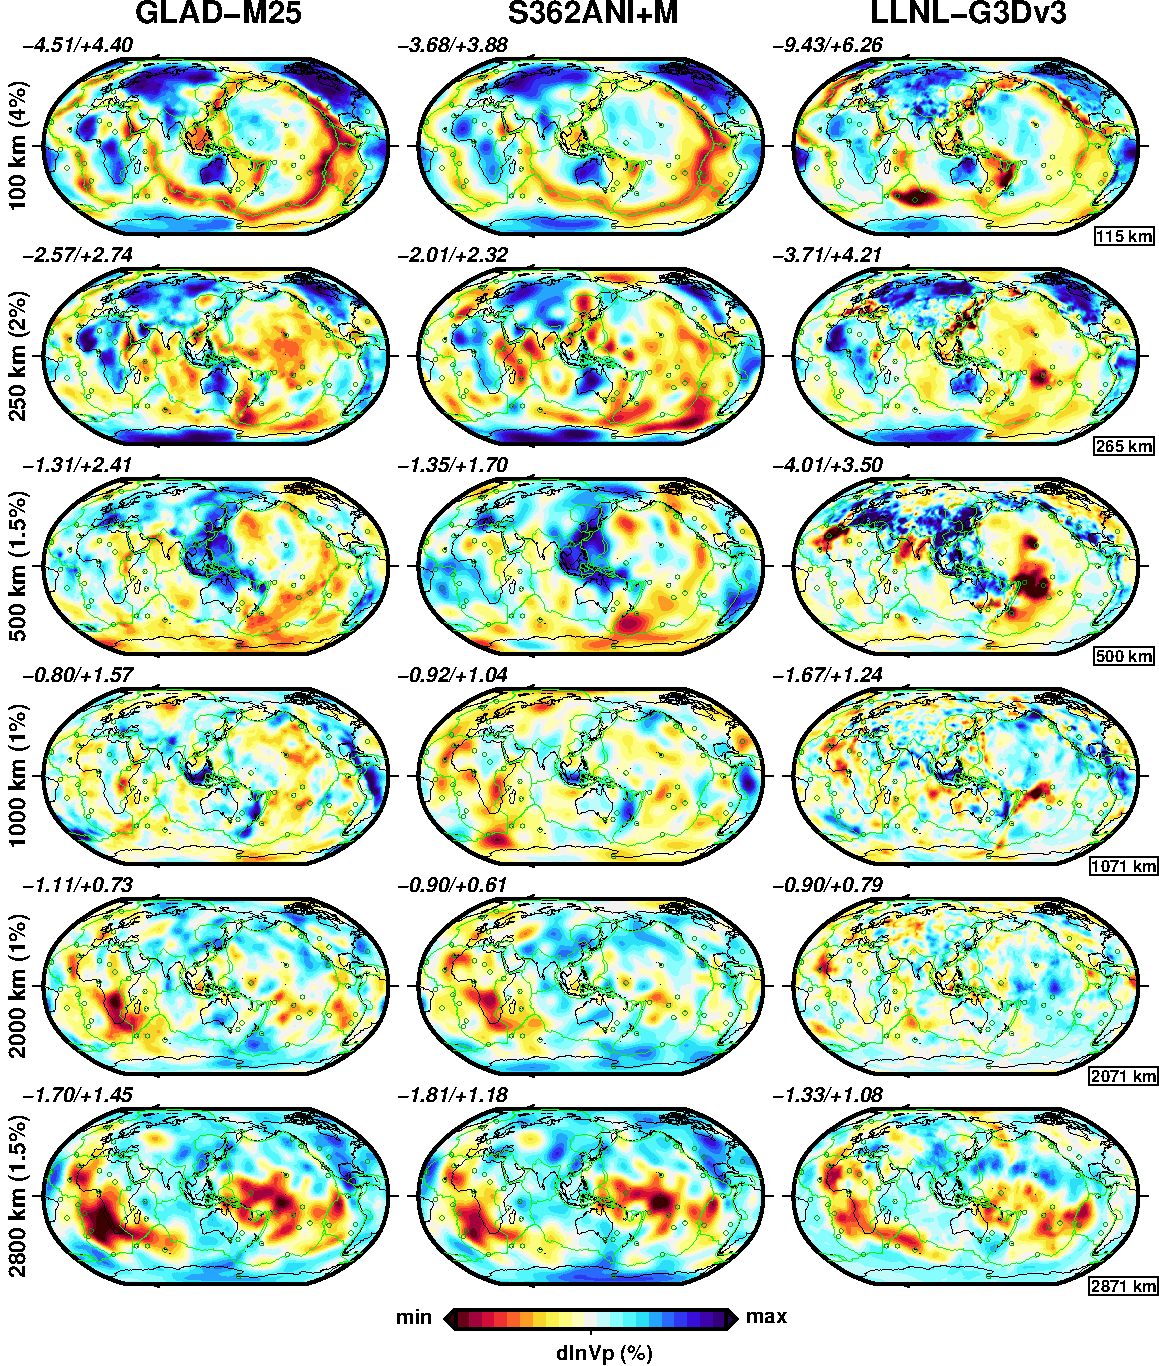
\includegraphics[width=0.9\textwidth]{ch-GLADM25/figures/depth_slice/globe_vp_S362ANI-LLNL.pdf}
%  \caption{\small{Map views of global $V_\textrm{P}$ variations at various depths for our model GLAD-M25(left column), S362ANI$+$M(middle column) and LLNL-G3Dv3(right column)\cite{simmons2012llnl}. For LLNL-G3Dv3, the depths is labeled on the right bottom based on its own mesh spacing. Other plotting conventions are used similar as in Figure \ref{fig:global-vs}.}}
%\label{fig:global-vp}
%\centering
%\end{figure

An important aspect of our inversion is that it constrains shear and
compressional waves simultaneously. In Fig.~\ref{fig:global-vs} we
compare global maps of our compressional wavespeed model with global P models
LLNL-G3Dv3~\cite{simmons2012llnl} and GAP-P4~\cite{fukao2013subducted}.
At a depth of 100~km,
GLAD-M25 shows prominent mid-oceanic ridges, cooling of the Pacific lithosphere,
and the roots of numerous continental cratons. In the upper mantle, LLNL-G3Dv3
exhibits the largest lateral variations,
e.g., very slow compressional wavespeeds at 500~km depth below Hawaii, Samoa, and Tahiti.
In the mid-mantle we can see remnants of subduction beneath South America, Indonesia,
and Tonga-Kermadec.
In the deep mantle, LLNL-G3Dv3 and GAP-P4 begin to fade out, but the long-wavelength patterns,
in particular the lower parts of the Africa and Pacific superplumes, are very similar.

\begin{figure}
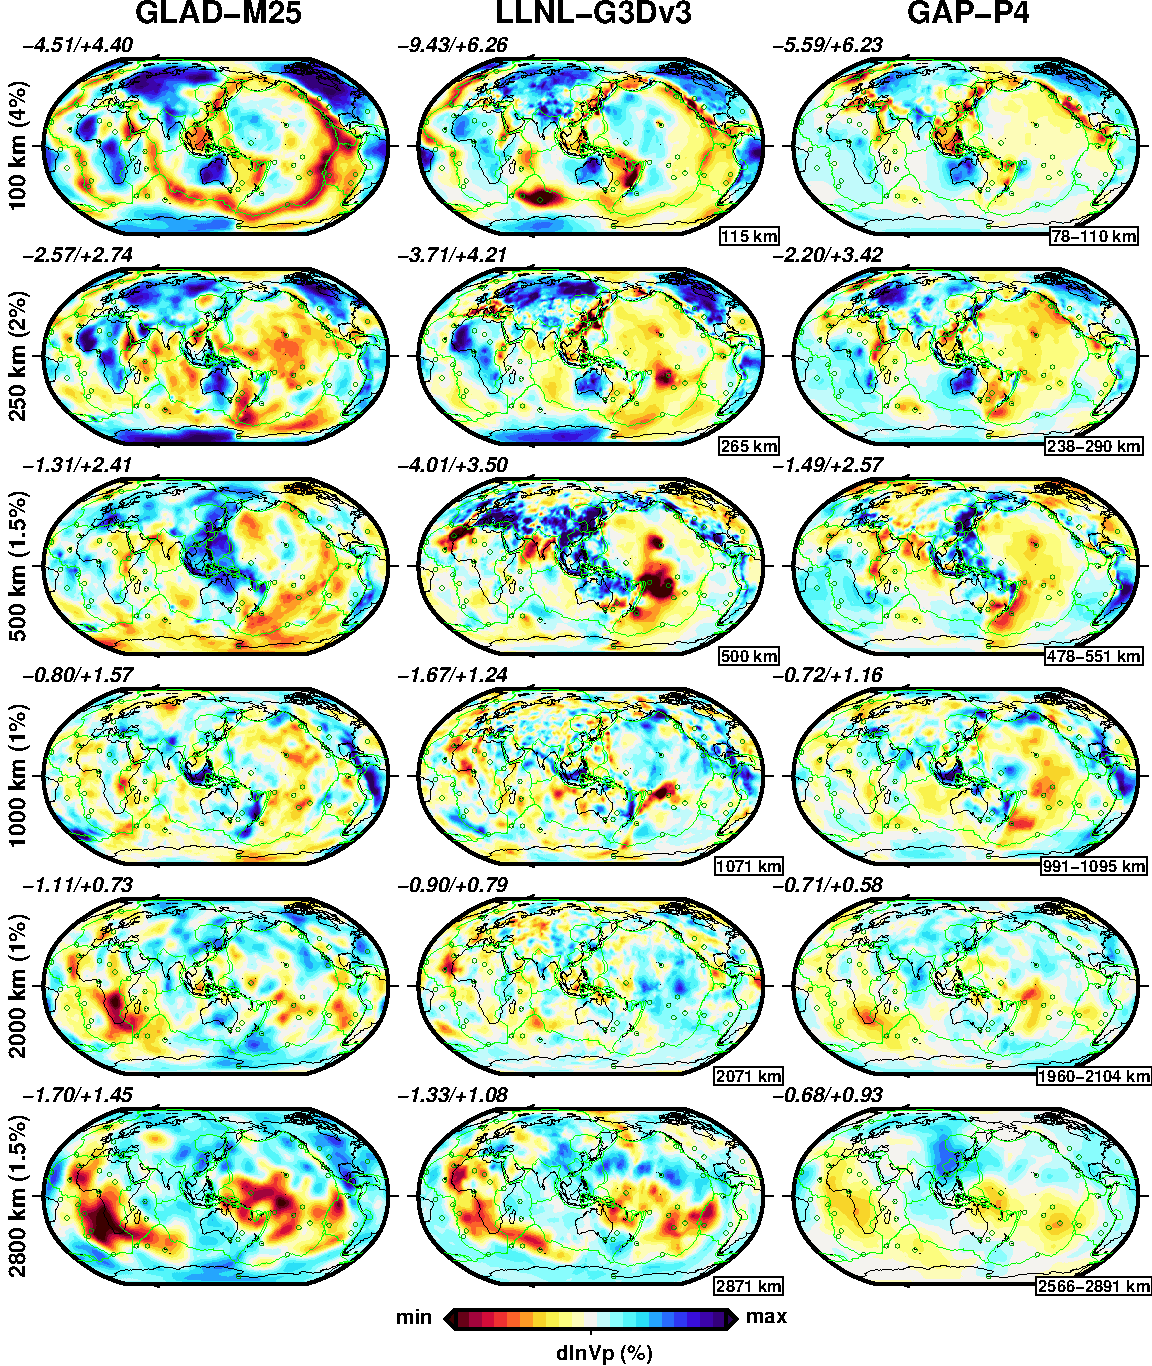
\includegraphics[width=0.9\textwidth]{ch-GLADM25/figures/depth_slice/globe_vp_LLNL-GAP.pdf}
  \caption[Map views of global compressional wavespeed variations at various depths]
  {\small{Map views of global compressional wavespeed variations at various depths for model
  GLAD-M25 (left column), LLNL-G3Dv3(middle column)\cite{simmons2012llnl}, and
  GAP-P4(right column)~\cite{fukao2013subducted}.
  For LLNL-G3Dv3, depth ranges are labeled in the bottom right
  bottom of each panel. Other plotting conventions are as in Fig.~\ref{fig:global-vs}.}}
\label{fig:global-vp}
\centering
\end{figure}

\subsubsection{North America}

\begin{figure}
\centering
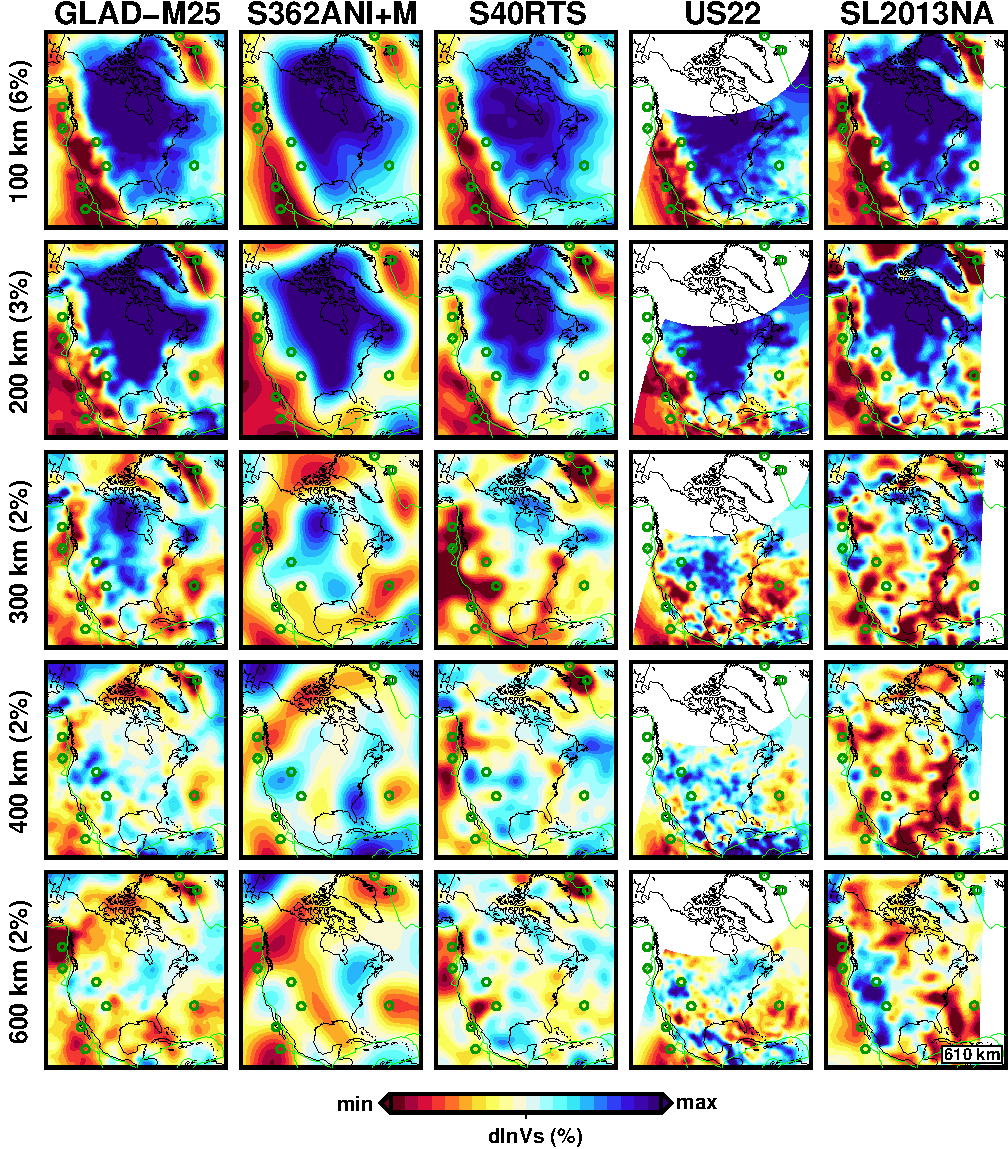
\includegraphics[width=0.9\textwidth]{ch-GLADM25/figures/depth_slice/america_vs.pdf}
  \caption[Map views of isotropic shear wavespeed variations beneath North America]
  {\small{Map views of isotropic shear wavespeed variations beneath North America 
  for model GLAD-M25 (first column) and several global (S362ANI$+$M and S40RTS)
  and regional US22~\cite{zhu2017radial} and SL2013NA~\cite{schaeffer2014imaging}
  models. Green circles denote the locations of hot-spots. For SL2013NA, we
  show a depth of 610~km instead of 600~km, reflecting its model parameterization.}}
\label{fig:america-vs}
\end{figure}

The deployment of USArray has dramatically increased data coverage across the
continental United States,
and yet despite this tremendous increase in data coverage, there is not as much overlap between different models as one might anticipate.
In this section, we compare GLAD-M25 in this region 
with two global models, S362ANI$+$M and S40RTS, and two regional models,
US22~\cite{zhu2017radial} and SL2013NA~\cite{schaeffer2014imaging}.
US22 is a radially anisotropic model based on adjoint tomography using
USArray data from 180 regional earthquakes using 15--50~s
body waves and 25--150~s surface waves.
SL2013NA is a global upper-mantle shear wavespeed model based on multimode
surface waveform tomography primarily focused on North America.

North America is characterized by a large, high-wavespeed lithospheric craton,
bounded by the Rocky Mountain Front to the West and continental
margin to the East~\cite{grand1984upper, whitmeyer2007tectonic}.
On both sides the lithosphere has been deformed by
low wavespeed structures, thus forming sharp tectonic boundaries
~\cite{masters1996shear, grand1997high, megnin2000three, gu2001models}.

At a depth of 100~km, we observe that the edges of the craton are sharper in
GLAD-M25 than in the other two global models,
and quite similar in shape and sharpness to the two regional models.
We can clearly see impressions of the Snake River Plain (with Yellowstone)
and the Raton hot-spot, which also have distinct slow expressions at depths of 200~km.
The core of the craton exhibits fast wavespeeds at depths reaching 300~km Northwest of
Hudson Bay.
In the regional models the craton has basically faded away at these depths.
The Wyoming and Medicine Hat Blocks show a very strong and thick lithospheric
root from shallow depths to $\sim$400~km, similar to US22 but
difficult to discern in SL2013NA.
Similar observations can be made for the Yavapai and
Mazatzal Blocks, which define the southern boundary of the large craton
~\cite{schaeffer2014imaging}.

In the 200--400~km depth range, we observe a high wavespeed
anomaly within the Gulf of Mexico, which coincides spatially with the deepest
bathymetry and corresponds to a portion of ancient oceanic
lithosphere~\cite{muller2008, schaeffer2014imaging}.
A remnant of the Juan de Fuca plate,
with a high wavespeed footprint, is visible at depths of 300~km and 400~km,
where SL2013NA shows a much stronger anomaly.

In the North, we see a high wavespeed craton beneath Greenland which is partly
separated from the North American craton by low wavespeed structures beneath
Baffin Bay and the Labrador Sea, where the North American craton nicely follows
the coastline~\cite{chalmers2001development}.
In the Northeast corner of the maps we see that the Iceland hot-spot is very
prominent in GLAD-M25 in all depth ranges, similar to S40RTS but largely missing
in S362ANI$+$M. In the Northwest we see a clear imprint of the Aleutian
subduction zone in the 200--400~km depth range, comparable to SL2013NA but absent
in the other global models.

In the East, at 100~km depth,
we see ageing of the Atlantic lithosphere, comparable to the other global models
~\cite{muller2008, schaeffer2014imaging}.
All models show fast anomalies beneath Newfoundland and Nova Scotia extending to
depths of 300~km. The Bermuda hot-spot shows a very nice slow wavespeed impression,
getting sharper and stronger at depths of 200~km and 300~km (note differences in
the scales of the maps).
The Caribbean slab, a relatively young subduction zone, is clearly
visible in our model in the 200--400~km depth range.
At greater depths,
GLAD-M25 shows a very distinct image of the Farallon slab,
but since it goes well beyond the depth range of this comparison,
we return to this feature in Section~\ref{section:slabs}.

\subsubsection{Europe}

\begin{figure}[ht!]
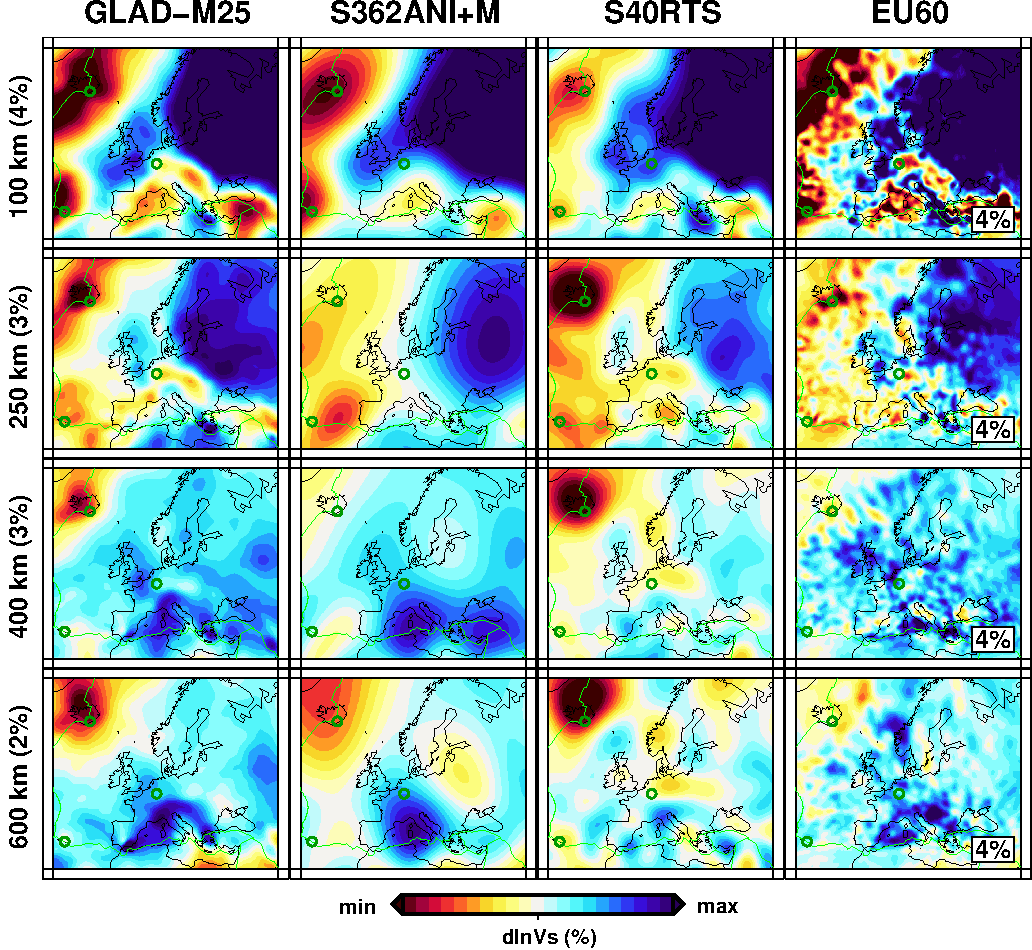
\includegraphics[width=0.9\textwidth]{ch-GLADM25/figures/depth_slice/europe_vs.pdf}
  \caption[Map views of isotropic shear wavespeed variations beneath Europe]
  {\small{Map views of isotropic shear wavespeed variations beneath Europe for model GLAD-M25 (first column), two global model (S362ANI$+$M and S40RTS), and
  one regional model EU60~\cite{zhu2015seismic}. For EU60, the range of the color
  bar is 4\% at all depths, as indicated in the bottom right bottom of the panels.}}
\label{fig:europe-vs}
\centering
\end{figure}

Fig.~\ref{fig:europe-vs} shows isotropic shear wavespeed perturbations beneath Europe.
In addition to models GLAD-M25, S362ANI$+$M, and S40RTS, we included regional
model EU60~\cite{zhu2015seismic} for comparison.
EU60 is the result of adjoint tomography of the crust and upper mantle
beneath the European continent and the North Atlantic based on the assimilation of data from
190 earthquakes recorded by 745 seismographic stations.

A defining tectonic feature of Europe is the Trans-European Suture Zone~(TESZ),
also known as the Tornquist-Teisseyre Zone,
separating the Precambrian East European Craton~(EEC) in the Northeast from
Phanerozoic Europe in the Southwest~\cite{zielhuis1994deep}.
The TESZ is very consistent across all models,
even though is much sharper in GLAD-M25 and EU60.

At depths of 100---250~km we observe high wavespeeds beneath the Central Graben
in the North Sea, which is clearly separated from the EEC.
The tectonic history of the Mediterranean is complex,
involving several regional plates and multiple past and present subduction zones
~\cite{dewey1989kinematics}.
We see slab ponding in the transition zone beneath the western Mediterranean
associated with slab roll-back of the Apennines-Maghrebides subduction zone
~\cite{wortel2000subduction, zhu2012structure}.
At shallower depths, we see low wavespeeds along its western border,
which are interpreted as back-arc extension associated with  roll-back.
Compared to S362ANI$+$M and S40RTS,
our model shows much sharper features for these tectonic structures.

In the Eastern Mediterranean, there is a distinct fast anomaly beneath the 
Dinarides Mountains, separating the Adria plate from the Pannonian Basin,
indicating subduction of the Adria plate beneath the Eurasian plate.
This anomaly gets sharper at 600~km depth.
Its southern part interacts with the Hellenic slab, which penetrates the mantle
transition zone and extends below 1,000~km in our model.
We discuss the Hellenic Arc further in Section~\ref{section:slabs}.
The Pannonian Basin is characterized by a low wavespeed
anomaly at depths from 100~km to 250~km.
In this depth range we also see slow wavespeeds beneath Anatolia,
stronger than in the two other global models.

In Central Europe we note the Cenozoic Ridge System~\cite{ziegler1992european},
characterized by low 
wavespeeds from the Massif Central to the Eifel. Both EU60 and
GLAD-M25 exhibit a slow anomaly beneath the northern part of the Rhine Graben,
which is interpreted as the reservoir that fuels the Eifel hot-spot
~\cite{goes1999lower, zhu2015seismic}.

Beneath the Atlantic Ocean, our model enhances slow anomalies beneath the
ridges, especially underneath Iceland and the Azores.
Compared to S362ANI$+$M, Iceland becomes much stronger in the upper mantle at
depths from 250~km to 400~km, extending all the way to the mantle-transition zone.
The Azores represent a much shallower hot-spot, with a maximum depth of about 250~km.

\subsubsection{Asia}

\begin{figure}[ht!]
  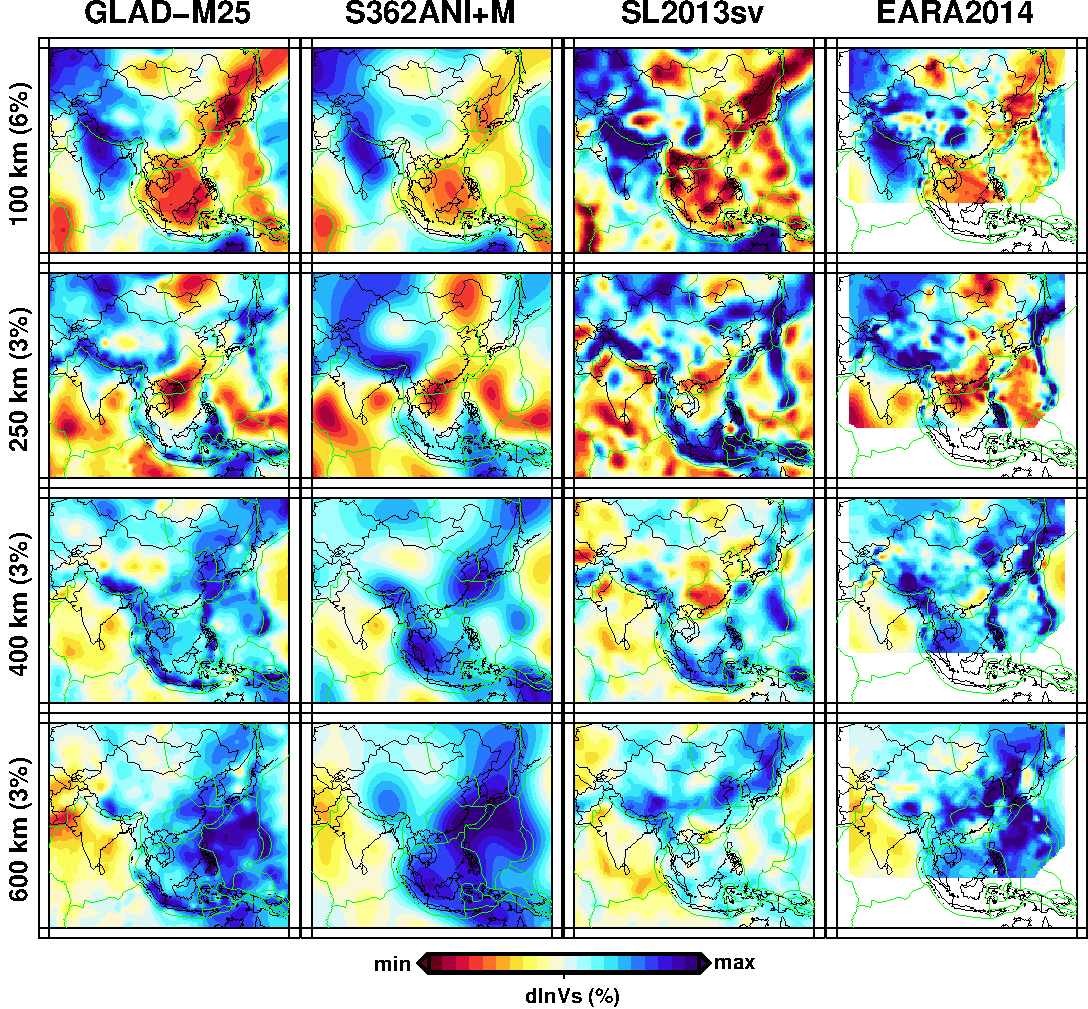
\includegraphics[width=0.9\textwidth]{ch-GLADM25/figures/depth_slice/asia_vs.pdf}
  \caption[Map views of shear wavespeed variations beneath Asia]
  {\small{Map views of shear wavespeed variations beneath Asia for GLAD-M25~(first column),
  global models S362ANI$+$M (second column) and SL2013sv (third column), and regional model EARA2014 (last column)~\cite{chen2015multiparameter}.}}
  \label{fig:asia-vs}
  \centering
\end{figure}

Asia, like Europe, has a complex tectonic history, involving
interactions among the Indian, Eurasian, Australian, Pacific, and Philippine
plates.
Map views of GLAD-M25 centered on Asia are plotted in Fig.~\ref{fig:asia-vs},
together with S362ANI$+$M, SL2013sv~\cite{SchaefferLebedev13}, and regional model EARA2014~\cite{chen2015multiparameter}.
EARA2014 is a transversely isotropic model based on adjoint
tomography, assimilating 1.7~million frequency-dependent traveltime
measurements from 227 earthquakes recorded by 1,869 seismographic  stations.
It has superior data coverage, mainly by incorporating data from the China Array.

The Southwestern part of China is dominated by the Himalayas,
expressing the collision between India and Eurasia~\cite{lebedev2003upper}.
GLAD-M25 exhibits strong high wavespeed anomalies in this area,
which extend all the way from 100~km to 600~km, narrowing and sharpening with depth,
in good agreement with EARA2014.
The Tibetan plateau shows relatively low wavespeeds
compared to its surroundings, including the Himalayas to its South and
the Tianshan Mountains to its North, consistent with the other global
and regional studies.

The southern part of Asia shows major tectonic activity between the
Philippine, Eurasian, and Australia plates.
The Sunda trench is visible as a distinct high wavespeed anomaly below 200~km,
nicely following the plate boundary.
This feature remains very sharp at 600~km and extends
down to 1000~km.
We discuss this subducting slab further in Section~\ref{section:slabs}.
The Manila and Philippine trenches are also much sharper in our model between 200~km and
600~km than in the other global models, and comparable to EARA2014.
The eastern edge of the map features a series of trenches following plate boundaries,
including Japan, Izu-Bonin, and Mariana.
These slabs are absent in the other global model,
but feature more prominently in EARA2014.
Along the northern edge we see low wavespeeds associated with the
Altai-Sayan and Baikal rift systems.
In terms of intra-plate activities,
at shallow depths we see clear low wavespeed impressions of the Hainan and Changbai volcanoes,
suggesting a lithospheric rather than deeper mantle origin~\cite{yin2000geologic}.
The Sichuan basin, a very localized high-wavespeed structure, extends below
250~km depth. At 600~km, most models shows a large region of high wavespeed
beneath the Philippine plate, indicating ponding of ancient subducted plates.

\subsubsection{South America}

\begin{figure}[ht!] 
  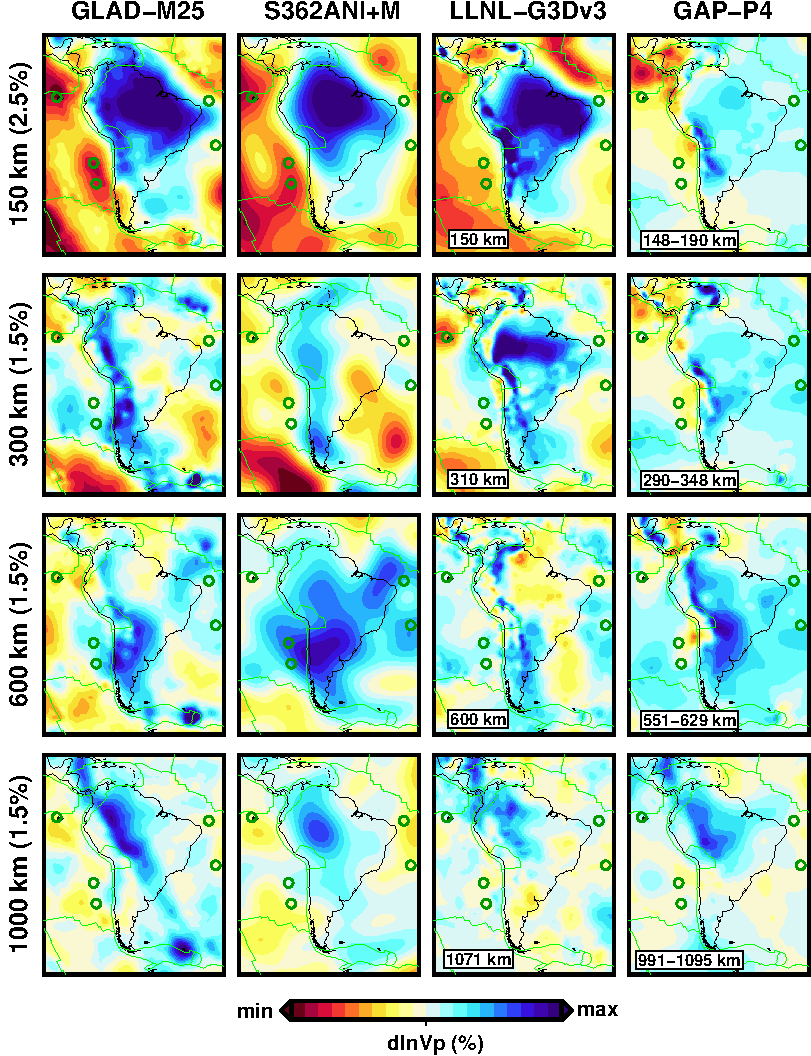
\includegraphics[width=0.9\textwidth]{ch-GLADM25/figures/depth_slice/south_america_vp.pdf}
  \caption[Map views of compressional wavespeed variations beneath South America]
  {\small{Map views of compressional wavespeed variations beneath South America for GLAD-M25~(first column) and global models S362ANI$+$M~\cite{moulik2014anisotropic} (second column), LLNL-G3Dv3~\cite{simmons2012llnl} (third column), and GAP-P4~\cite{fukao2013subducted} (fourth column).}}
  \label{fig:southamerica-vp}
  \centering
\end{figure}

Fig.~\ref{fig:southamerica-vp} shows compressional wavespeed anomalies in model GLAD-M25 in comparison with three
global models, namely, S362ANI$+$M~\cite{moulik2014anisotropic}, LLNL-G3Dv3~\cite{simmons2012llnl}, and GAP-P4~\cite{fukao2013subducted};
the latter two are $V_\textrm{P}$ models.

At 150~km depth, the northern half of South America is covered by a large lithospheric craton, exhibiting fast anomalies in all models except GAP-P4.
The Galapagos,
San Felix, and Juan Fernandez hot-spots are associated with distinct low wavespeed anomalies in GLAD-M25,
but not in the other models.
At 300~km depth, we see sharpened subduction of the Nazca plate
in GLAD-M25 compared to S362ANI+M, similar in shape to model LLNL-G3Dv3.
Moving to greater depths,
we see distinct Peru and Chile slabs in GLAD-M25,
with the Chile slab ponding in the transition zone
and the Peru slab penetrating into the lower mantle and still clearly visible at 1000km depth.
These differences in behavior are consistent with GAP-P4
\cite{fukao2013subducted}.

In the south,
Scotia Arc subduction is very distinct in GLAD-M25 at all depths,
but barely observable in other models.
This is probably a consequence of coverage provided by events in the region (see Fig.~\ref{fig:event_1480}).
To the north,
Caribbean subduction is clearly discernible in model GLAD-M25 and the two $V_\textrm{P}$ models.

\subsection{Plumes}
\label{section:plumes}

\begin{figure}[ht!]
  \centering
  \sidesubfloat[]{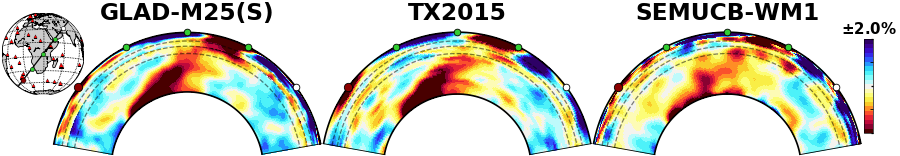
\includegraphics[width=0.98\textwidth]{ch-GLADM25/figures/plumes/Afar.png}}\\[-1pt]
  \sidesubfloat[]{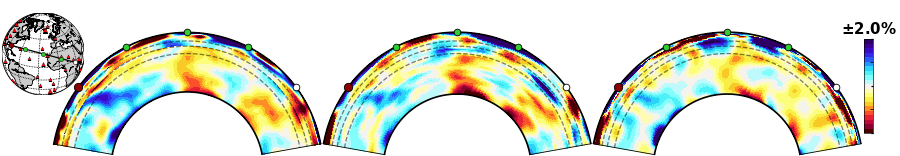
\includegraphics[width=0.98\textwidth]{ch-GLADM25/figures/plumes/Bermuda_Canary.png}}\\[-1pt]
  \sidesubfloat[]{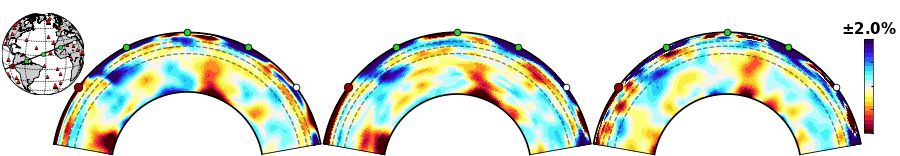
\includegraphics[width=0.98\textwidth]{ch-GLADM25/figures/plumes/CapeVerde_Hoggar.png}}\\[-1pt]
  \sidesubfloat[]{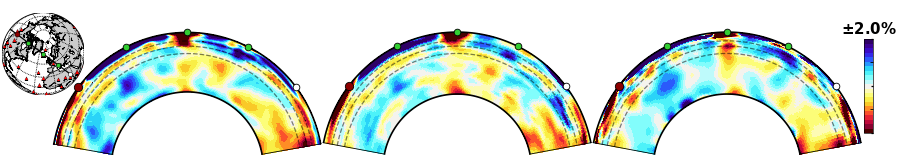
\includegraphics[width=0.98\textwidth]{ch-GLADM25/figures/plumes/Iceland_Eifel.png}}\\[-1pt]
  \sidesubfloat[]{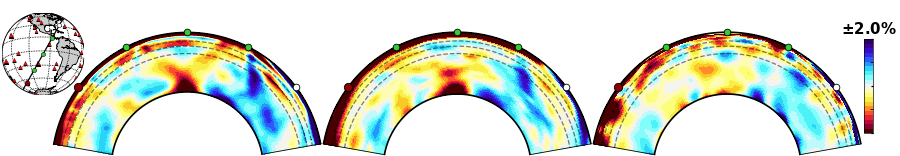
\includegraphics[width=0.98\textwidth]{ch-GLADM25/figures/plumes/Easter_Galapagos.png}}\\[-1pt]
  \sidesubfloat[]{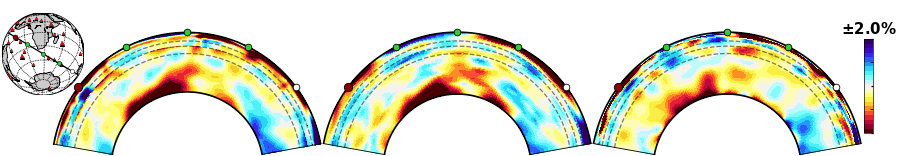
\includegraphics[width=0.98\textwidth]{ch-GLADM25/figures/plumes/Marion3_Kerguelen.png}}\\
  \caption[Vertical cross sections of shear wavespeed perturbations for various plumes]
    {\small{Vertical cross sections for various plumes for models GLAD-M25 ($V_\textrm{S}$; left column),
    TX2015~\cite{TX2015} (center column), and SEMUCB-WM1~\cite{french2015broad} (right column).
    The map in the top left corner of each row shows the cross section with color-coded red, green,
    and white dots for geographical reference;
    hot-spots are denoted by red triangles.
    The dashed black semicircles in the cross sections denote depths of 410~km, 660~km, and 1000~km.
    (a) Afar; (b) Bermuda (left) and Canary (middle); (c) Cape Verde (middle) and Hoggar (right);
    (d) Iceland (middle) and Eifel (right); (e) Easter (left) and Galapagos (right); (f) Marion (middle),
    and Kerguelen (right). }}
  \label{fig:plumes_combo}
\end{figure}

In this section we highlight various plume systems on Earth. Fig.~\ref{fig:plumes_combo}
shows cross sections of several plumes, comparing models GLAD-M25 ($V_\textrm{P}$),
TX2015~\cite{TX2015}, and SEMUCB-WM1~\cite{french2015broad}.
All three models have common plume features,
and GLAD-M25 and TX2015 are in overall good agreement.  

The three models tend to agree near the CMB,
and there is overall good agreement between GLAD-M25 and TX2015,
but the models can differ substantially in the mid and upper mantle,
with profoundly different implications for mantle
convection.

\begin{itemize}
\item[]{\it Afar} In Fig.~\ref{fig:plumes_combo}(a),
we see that the Afar plume in model GLAD-M25 originates from the CMB, narrows its diameter
in the mid mantle, and broadens again above the 660~km discontinuity.
It exhibits
very similar behavior in TX2015 but differs significantly in SEMUCB-WM1.  
\item[]{\it Bermuda and Canary} In Fig.~\ref{fig:plumes_combo}(b), from left to right, we see in model GLAD-M25 (i) the Farallon
slab; (ii) the Bermuda hot-spot above the 660~km discontinuity; (iii) the Canary hot-spot originating from the CMT and
rising all the way up the Earth's surface; (iv) the Afar hot-spot from another angle.
\item[]{\it Cape Verde and Hoggar} Fig.~\ref{fig:plumes_combo}(c) features (i) South America subduction; (ii) the Cape Verde hot-spot extending from the CMB all the way to the surface; (iii) the Hoggar hot-spot from 660~km to the surface. 
\item[]{\it Iceland and Eifel} Fig.~\ref{fig:plumes_combo}(d) shows a plume which rises from the CMB right below Iceland, reaches 660~km, amplifies,
and ascends to the surface.
The intensification above 660~km may be an indication of partial melting.
\item[]{\it Easter and Galapagos} Fig.~\ref{fig:plumes_combo}(e) contains (i) the Easter hot-spot; (ii) the Galapagos
hot-spot; (iii) the Central America slab.
In models GLAD-M25 and TX2015,
the Easter and Galapagos hot-spots appear to originate from the same underlying plume in the deep mantle,
which is the eastern arm of the Pacific superplume.
\item[]{\it Marion and Kerguelen}
Finally,
in Fig.~\ref{fig:plumes_combo}(f) we see the Marion and Kerguelen hot-spots, which might be connected to Afar in the lower mantle.
Recovering these plumes is challenging due to poor data coverage in the southern hemisphere.
\end{itemize}

%\begin{figure}
%    \centering
%    \sidesubfloat[]{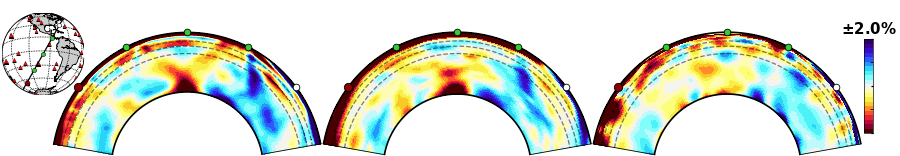
\includegraphics[width=0.98\textwidth]{ch-GLADM25/figures/plumes/Easter_Galapagos.png}\label{fig:a}}\\[-1pt]
%    \sidesubfloat[]{\includegraphics[width=1.0\textwidth]{ch-GLADM25/figures/plumes/Macdonald_Yellowstone.png}\label{fig:b}}\\[-1pt]
%    \sidesubfloat[]{\includegraphics[width=1.0\textwidth]{ch-GLADM25/figures/plumes/Pitcairn_Guadalupe.png}\label{fig:c}}\\[-1pt]
%    \sidesubfloat[]{\includegraphics[width=1.0\textwidth]{ch-GLADM25/figures/plumes/Samoa_Hawaii.png}\label{fig:d}}\\[-1pt]
%    \sidesubfloat[]{\includegraphics[width=1.0\textwidth]{ch-GLADM25/figures/plumes/Samoa_MarquesasS1.png}\label{fig:e}}\\[-1pt]
%    \sidesubfloat[]{\includegraphics[width=1.0\textwidth]{ch-GLADM25/figures/plumes/Tahiti_Macdonald.png}\label{fig:f}}\\
%    \caption{\small{Vertical cross sections of shear wave velocity perturbations of plumes in the pacific region.}}
%\end{figure}

\subsection{Subduction zones}
\label{section:slabs}

\begin{figure}
    \centering
    \sidesubfloat[]{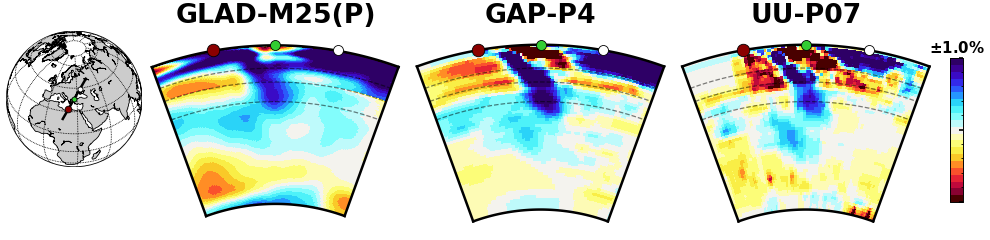
\includegraphics[width=0.88\textwidth]{ch-GLADM25/figures/subductions/Aeg.png}\label{fig:subd_a}}\\[-8pt]
    \sidesubfloat[]{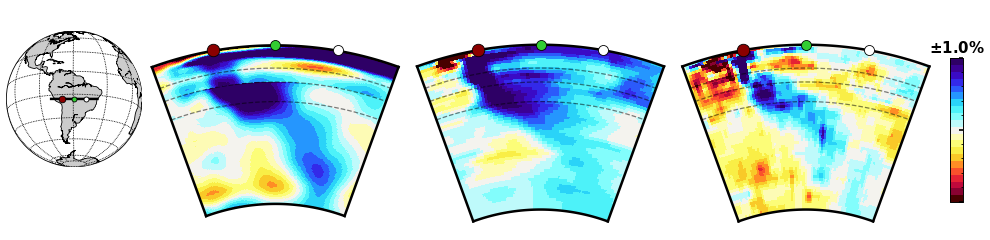
\includegraphics[width=0.88\textwidth]{ch-GLADM25/figures/subductions/Br.png}\label{fig:subd_b}}\\[-8pt]
    \sidesubfloat[]{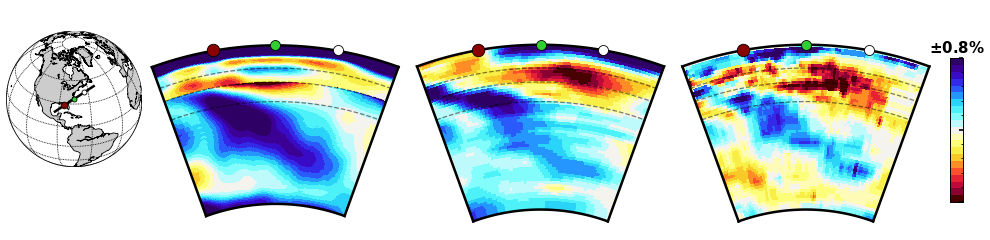
\includegraphics[width=0.88\textwidth]{ch-GLADM25/figures/subductions/Ha.png}\label{fig:subd_c}}\\[-8pt]
    \sidesubfloat[]{\includegraphics[width=0.88\textwidth]{ch-GLADM25/figures/subductions/Wc.png}\label{fig:subd_e}}\\[-8pt]
    \sidesubfloat[]{\includegraphics[width=0.88\textwidth]{ch-GLADM25/figures/subductions/Ne.png}\label{fig:subd_d}}\\[-8pt]
    \sidesubfloat[]{\includegraphics[width=0.88\textwidth]{ch-GLADM25/figures/subductions/Su.png}\label{fig:subd_f}}\\[-8pt]
    \caption[Vertical cross sections of compressional wavespeed perturbations in various subduction zones]
    {\small{Vertical cross sections of compressional wavespeed perturbations in various subduction zones
    for models GLAD-M25 ($V_\textrm{P}$; left column), GAP-P4~\cite{fukao2013subducted} (middle column) and UU-P07~\cite{van2018atlas} (right column).
    The map in the top left corner of each row shows the cross section with color-coded red, green, and white dots for geographical reference.
    The dashed black semicircles in the cross sections denote depths of 410~km, 660~km, and 1000~km.
    (a)~Aegean; (b)~South America; (c)~Hatteras; (d)~Wichita. (e)~Nepal; (f)~Sunda.}}
    \label{fig:subd_combo}
\end{figure}

In this section we highlight various subduction systems on Earth.
In Fig.~\ref{fig:subd_combo} we compare GLAD-M25~($V_\textrm{P}$) with two compressional wavespeed models,
namely, GAP-P4~\cite{fukao2013subducted} and UU-P07~\cite{van2018atlas}.
Fig.~\ref{fig:subd_combo}(a) features the Aegean subduction zone. All models show a slab penetrating into the lower mantle beyond a depth of 1,000~km.
Fig.~\ref{fig:subd_combo}(b) shows the South American slab, which, in this cross section, ponds in the shallow lower mantle in all three models, before sinking all the way to the CMB.
Figs.~\ref{fig:subd_combo}(c) and~(d) show cuts across the ancient Farallon slab, which penetrates deeply into the lower mantle,
as spectacularly documented by, for instance, \cite{grand1994,hilst1997,grand1997high}.
At depths greater than 1,000~km, 
we see a very strong expression of the slab in model GLAD-M25, which is much weaker in the two P models.
The difference may be attributed to increased data coverage thanks to USArray, as well as the use of finite-frequency Fr\'echet derivatives.
Fig.~\ref{fig:subd_combo}(e) shows subduction beneath the Himalayas.
All three models show two distinct fast anomalies below 660~km,
one above 1,000~km and the other, further to the southwest, below 1,000~km.
Finally, Fig.~\ref{fig:subd_combo}(f) shows subduction beneath the Java portion of the Sunda Arc.
At this location the slab penetrates into the lower mantle, at which point its spreads out laterally,
in agreement with models GAP-P4 and UU-P07.
\cite{fukao1992} explained this flattening using a model of~\cite{ringwood1988},
suggesting that the subducted slab thickened and buckled to form a dense megalith
above the 660~km discontinuity before sinking into the lower mantle.

Overall, the three models are in reasonably good agreement.
At shallow depths, model GLAD-M25 shows more distinct continental crust and cratons, thanks to the inclusion of surface waves.
But in the upper and mid mantle,
the models share very similar attributes.

\section{Discussion}

Seismology is a science driven by data.
There was a time when global seismologists would meticulously inspect single seismograms to glean valuable information from them.
Today, we have easy access to data from thousands of earthquakes recorded by tens of thousands of seismographic stations, and individual inspection of all of these records has become impossible.
Still, it would be a shame not to utilize as much as possible of the information in this massive seismographic database.

To facilitate fast and effective access to such vast data resources,
we use ASDF~\cite{krischer2016adaptable} in the preprocessing stage of the adjoint tomography workflow,
and to accommodate massive I/O during the postprocessing stage we use the ADIOS library~\cite{liu2014hello}.
For data assimilation,
tools such as FLEXWIN, which automatically select data windows suitable for measurements, are indispensable, and we see tremendous opportunities for the use of machine learning algorithms in this context~\cite{chen2017}.
Without these libraries and tools, the construction of model GLAD-M25 would have been impossible. 

Some form of automated parallel workflow management is critical for the global adjoint tomography process,
because classical inversion workflows suffer from I/O inefficiencies, lack of fault tolerance, and an inability to work in distributed resource environments~\cite{Lefebvre2018}.
The EnTK workflow management engine~\cite{EnTK2017}
largely overcomes these limitations by facilitating tracking of tasks and job failure detection,
thereby enabling semi-automatic job resubmission if necessary.
These are the attributes required for bringing global FWI to its full potential,
enabling the assimilation of data from thousands of earthquakes on the largest HPC systems.

It should be clear from this discussion that modern seismic tomography requires close collaborations with computational scientists, HPC specialists, and visualization experts,
as reflected in the list of authors for this article, in addition to access to the most advanced computational platforms,
such as those offered through the DOE INCITE and NSF XSEDE programs.

Although Figs.~\ref{fig:window_density_Z}--\ref{fig:window_density_T} illustrate that much information in seismograms is
being assimilated, we still have a long way to go before explaining every wiggle in hundreds-of-minutes-long seismograms.
Currently, we are only fitting the phase in selected time windows, and amplitude information remains completely unused.
We accommodate the full physics of seismic wave propagation,
but we are not exploiting the most general earth model parameterization.
GLAD-M25 is an elastic model with radial anisotropy confined to the upper mantle.
It is well known that the upper mantle is azimuthally anisotropic~\cite{montagner1989petrological,montagner1991},
and we also know that amplitude information helps constrain second derivatives in phase speed~\cite{WW86,TDI,TDII},
in addition to lateral variations in attenuation~\cite{romanowicz1998,reidetal2001,DaEkDz08}.
Thus, the natural next step in global FWI is to use phase and amplitude information simultaneously to jointly constrain the elastic and anelastic structure of the Earth.
To accomplish this next step, source parameters need to be constrained more carefully, especially as we push the resolution to shorter periods~\cite{valentine2010}.

The global distribution of earthquakes (Fig.~\ref{fig:event_1480}) and stations (Fig.~\ref{fig:stations}) is highly uneven.
This problem may be alleviated to some extent by using suitably chosen misfit functions with appropriate geographical weighting of sources and receivers~\cite{Li1996,Ruanetal2018}.
The ultimate solution may be a dense network of Ocean Bottom Seismometers,
but meanwhile an armada of floating seismometers may offer a cheaper and more practical alternative~\cite{Nolet19}.

\section{Conclusion}

Building on our experiences during the construction of our first-generation global adjoint tomography model GLAD-M15~\cite{bozdaug2016global},
for this study we expanded our earthquake database from 253 to 1,480 events,
which were collectively recorded by more than 11,000 seismographic stations.
We used three-component seismograms in four period bands,
namely 17--40~s body waves, 40--100~s body waves, 40--100~s surface waves, and 90--250~s surface waves,
resulting in twelve measurement categories.
This culminated in the assimilation of more than 18~million time windows.

GLAD-M25 --- like its predecessor GLAD-M15 --- invokes no crustal corrections, and constrains crust and mantle shear and compressional wavespeeds simultaneously.
Such ubiquitous crustal corrections may affect inferences about upper-mantle anisotropy~\cite{BozdagTrampert2008,PaLeRo10,Ferreira10}, and are likely the main reason for significant differences between radially anisotropic upper-mantle models~\cite{Chang14}.
Treating the crust and mantle equally and simultaneously is one of the main strengths of GLAD-M25, accepting the additional computational costs, but thereby avoiding any approximations or corrections.
Another strength is the fact that the effects of attenuation are fully accommodated, both in forward and in adjoint simulations.
These points highlight the importance of taking the full physics of seismic wave propagation properly into account in seismic imaging. 

Another very important attribute of GLAD-M25 is that it constrains shear and compressional wavespeeds simultaneously in the same period range,
thereby enabling us to interpret the two wavespeeds together.
As illustrated in Figs.~\ref{fig:window_density_Z} and~\ref{fig:window_density_R},
numerous compressional wave arrivals are assimilated, including P, PP, PPP, PKP, PS, and PPS.
In future work we will capitalize on this by using the $V_\text{P}/V_\text{S}$ ratio to help constrain thermo-chemical and geodynamical processes in the mantle.

GLAD-M25 was quantitatively evaluated in several ways.
First, it produces significant misfit
reductions in all twelve measurements categories.
Second,
it produces nicely-centered Gaussian traveltime \& amplitude anomaly histograms
in all measurement categories.
Finally,
for a held-out data set of 360 events
we see similar misfit reductions and traveltime \& amplitude anomaly histograms as in the actual inversion.

When we compare GLAD-M25 with other global models,
we find overall good agreement at longer wavelengths.
In particular, GLAD-M25 and TX2015 feature very similar plume structures.
Unlike other global models, when we compare GLAD-M25 with regional models
we also observe generally good agreement at smaller wavelengths,
and, in particular, plumes and subduction zones feature prominently.
However, it is important to note that GLAD-M25 tends to agree well with regional models based on the same S362ANI~$+$~Crust2.0 starting model, numerical wave propagation solver, and quasi-Newton inversion technique (e.g., EU60, US22, and EARA2014).
It is also important to point out that even in regions with dense seismographic coverage, such as North America,
recent models can differ substantially, especially at greater depths.
Nevertheless, our global inversion is bridging the gap between global and regional studies,
approaching regional-scale resolution is areas with sufficient data coverage.
We can observe this increase in resolution in GLAD-M25 in the normalized power per spherical harmonic degree as a function of radius, which is displayed in Fig.~\ref{fig:powerspectraradius}.

\begin{figure}
  \centering
  \includegraphics[width=0.95\textwidth]{ch-GLADM25/figures/power_radius.pdf}
  \caption[Normalized power spectrum]
  {\small{Normalized power per degree~$\ell$ as a function of radius, based on Eqn.~(\ref{eq:powerdegreeradius}), for models S362ANI (left), GLAD-M15 (middle), and GLAD-M25 (right).
  Shown are depths greater than 120~km.
  (Courtesy of Caio Ciardelli.)
  }}
  \label{fig:powerspectraradius}
\end{figure}

% \begin{figure}
%   \centering
%   \includegraphics[width=0.95\textwidth]{ch-GLADM25/figures/power_radius2.pdf}
%   \caption{\small{Normalized power per degree~$\ell$ as a function of radius, based on Eqn.~(\ref{eq:powerdegreeradius}), for models S362ANI (first column), S40RTS (second column), GLAD-M15 (third column), and GLAD-M25 (fourth column).
%   Shown are depths greater than 120~km.
%   (Courtesy of Caio Ciardelli.)
%   }}
%   \label{fig:powerspectraradius}
% \end{figure}

Obvious future directions of research include growing the earthquake database further to the roughly 6,000 earthquakes in the right magnitude range already available via the Global CMT database,
and reducing the shortest simulation period further from 17~s to 8.5~s.
The most recent machine at OLCF, called ``Summit'', uses IBM Power9 CPUs accelerated by NVIDIA Tesla V100 GPU and can readily accommodate such simulations.

Other future directions of research involve inversions for azimuthal anisotropy
and attenuation.
The feasibility of such inversions on a regional scale has already been demonstrated in studies focused on Europe by~\cite{ZhuTromp2013} and \cite{Zhuetal2013}.

\section{Acknowledgments}
This research used resources of the Oak Ridge Leadership Computing Facility,
which is a DOE Office of Science User Facility supported under contract DE-AC05-00OR22725.
Additional computational resources were provided by the Princeton Institute
for Computational Science \& Engineering (PICSciE).
We acknowledge IRIS ({\tt iris.edu}) and ORFEUS ({\tt orfeus-eu.org}) for
providing the data used in this study.
We thank Ryan Modrak, Ridvan \"{O}rsvuran, Frederik J.\ Simons, and James Smith for fruitful discussions,
and Caio Ciardelli for implementing the spherical harmonic model expansion.
The open source spectral-element software package SPECFEM3D\_GLOBE and
the seismic measurement software package FLEXWIN used for this article are
 freely available via the Computational Infrastructure for Geodynamics
 (CIG; {\tt geodynamics.org}).
 This research was supported by NSF grant~1644826.


In this work, we explain how to use the puthesis.cls class file and the accompanying template.  


%
\chapter{Related Work\label{ch:pastwork}}

Everyone needs a chapter about related work, so here is a placeholder.

% include other files for sections of this chapter. These use the 'input' command since each section within a chapter should not start a new page.
% If you want to swap the order of sections, it is as simple as reversing the order you include them. 
\section{Tables}
\label{sec:pastwork:tables}

Tables are also quite important. Any table that can fit entirely on one page can be a floating table. If a table is longer and will span multiple pages, a long table can be inserted in-line with the text. This is demonstrated in Table~\ref{tab:usage:options}, and explained in Appendix~\ref{ch:implementation}.

Tables that fit on one page use normal floating figures. Keep the 'p' placement option (in addition to 'h' and 't') so that if the float cannot fit in-line with the document text, it can be on a separate page by itself immediately after it is placed. Without the 'p' option, the float may get pushed to the end of the chapter, along will all other floats in the chapter that follow it.

Table~\ref{table:pastwork:publishing} lists the various options for publishing your dissertation, with costs, as of 2010. You will have to bring a check for the appropriate amount, made out to ``Princeton University Library'', when you submit your bound dissertation copies to Mudd Library, along with the appropriate forms and the electronic copy of your dissertation burned to a CD (not a DVD) as a single PDF file. (See~\cite{muddthesis2009}.)

Traditional publishing is cheaper initially and lets you earn royalties if the publisher sells many copies of your dissertation. However, most of us won't have a best-seller dissertation and most likely won't earn royalties anyway. Instead, by choosing open access publishing, your dissertation will be available online for free to anyone who is interested. I strongly advocate for open access, to maximize the impact of your research.

Your dissertation is protected by copyright regardless of whether or not you have the copyright registered. However, registration establishes a public record of your copyright claim~\cite{muddthesis2009}. ProQuest will submit the copyright registration for an extra fee (about \$55). Alternatively, you can register it yourself at the Copyright Office's website for only \$35: \url{http://www.copyright.gov/eco/}.

\begin{table}[htbp]
\centering
\caption[Thesis Publishing Options]{Thesis publishing options~\cite{mudd2009}, as of May 2010. }
\label{table:pastwork:publishing}
\begin{tabular}{p{0.3\textwidth} p{0.15\textwidth} p{0.15\textwidth} p{0.15\textwidth} p{0.15\textwidth}}
\toprule
\textbf{Publishing Method} & \textbf{Publishing Fee}
 & \textbf{Diploma Fee} & \textbf{Copyright Registration Fee} & \textbf{Total} \\
\midrule
\multicolumn{5}{c}{Traditional Publishing}\\
\midrule

Traditional without copyright registration
& 65 & 15 & -- & 80 \\[0.2em]

Traditional with copyright registration
& 65 & 15 & 55 & 135 \\[0.2em]

\midrule
\multicolumn{5}{c}{Open Access}\\
\midrule

Open access without copyright registration
& 160 & 15 & -- & 175 \\[0.2em]

Open access with copyright registration
& 160 & 15 & 55 & 230 \\

\bottomrule
\end{tabular}
\end{table}
\section{Figures}
\label{sec:pastwork:figures}

Everyone needs floating figures in their dissertation. 

As shown in Figure~\ref{fig:pastwork:titlepage}, the Mudd Library dissertation requirements~\cite{muddthesis2009} specify additional options for formatting the title page. For example, if your thesis has multiple volumes, or to indicate the proper formatting for a master's thesis.

\begin{figure}[htb]
  \begin{center}
    \includegraphics[width=0.9\linewidth]{ch-pastwork/figures/titlepage}
    \caption[Sample Title Page Layout]{Sample title page layout~\cite{muddthesis2009}}
    \label{fig:pastwork:titlepage}
  \end{center}
\end{figure}



%
\chapter{Usage\label{ch:usage}}

To start, in your main .tex file, use this class as your main documentclass instead of `report' or `book'. For example:
\begin{quote}
$\backslash documentclass[12pt,lot, lof]\{puthesis\}$
\end{quote}

In this example, we setup our document to use the PU Thesis style, with 12pt font for body text, and to include a List of Tables and List of Figures in the front matter. You could instead set an 11 point or 10 point font by changing the first option. You can also add `los' to include a list of symbols.

To use single spacing, add the option `singlespace'. This is a special option for the \texttt{puthesis} documentclass, which sets single spacing for both the front matter and for the document itself. Additional parameters should be set in your main .tex file, and are described in detail in Section~\ref{sec:usage:options}.

The template itself declares two other options, to be set immediately after the \texttt{documentclass} command. First is `printmode', declared with the command:
\begin{quote}
$\backslash newcommand\{\backslash printmode\}\{\}$
\end{quote}
This command, used later in the thesis.tex file, turns off the \texttt{hyperref} package and all internal links in the PDF file. This removes any colored links and highlighting that would not be appropriate in a printed and bound thesis. Instead the \texttt{url} package is loaded, so that \\url commands in your document will continue to work and urls will break properly across multiple lines.

When `printmode' is not specified, the hyperref package is included. It creates colored links for citations, footnotes, and internal references, which can be used to navigate the PDF document more easily. It also adds bookmarks to the PDF file, mirroring the table of contents. By default, it is set to use colored links. For the PDF file that you will submit electronically to ProQuest, this may not be desirable since some copies may be printed, while others will be used electronically. Thus another option, `proquestmode', is defined that keeps hyperref but disables colored links:
\begin{quote}
$\backslash newcommand\{\backslash proquestmode\}\{\}$
\end{quote}
This mode has no effect when used in combination with `printmode'. 


\section{Options}
\label{sec:usage:options}

In this section, we describe the options you can set when using this thesis class.
\tablespacing
% tablespacing is defined by the class to set single spacing for the long table when in doublespacing mode. If the singlespace option is set, this command has no effect.

\begin{longtable}{p{0.3\linewidth} p{0.6\linewidth}}

  % First page heading
  \caption[Options Provided by the PUthesis Class]{List of options for the puthesis document class and template} \label{tab:usage:options}\\
  \toprule
  \textbf{Option} & \textbf{Description} \\
  \midrule
  \endfirsthead

  % Future page heading
  \caption[]{(continued)}\\
  \toprule
  \textbf{Option} & \textbf{Description} \\
  \midrule
  \endhead

  % Page footer
  \midrule
  \multicolumn{2}{r}{(Continued on next page)}\\
  \endfoot

  % Last page footer
  \bottomrule
  \endlastfoot

  12pt &
  Specify the font size for body text as a parameter to \texttt{documentclass}. The Mudd Library requirements~\cite{muddthesis2009} state that 12pt is preferred for serif fonts (e.g., Times New Roman) and 10pt for sans-serif fonts (e.g., Arial).
  \\

  letterpaper &
  If your document is coming out in a4paper, your LaTeX defaults may be wrong. Set this option as a parameter to \texttt{documentclass} to have the correct 8.5"x11" paper size.
  \\

  lot &
  Set this option as a parameter to \texttt{documentclass} to insert a List of Tables after the Table of Contents.
  \\


  lof &
  Set this option as a parameter to \texttt{documentclass} to insert a List of Figures after the Table of Contents and the List of Figures.
  \\

  los &
  Set this option as a parameter to \texttt{documentclass} to insert a List of Symbols after the Table of Contents and the other lists.
  \\

  singlespace &
  Set this option as a parameter to \texttt{documentclass} to single space your document. Double spacing is the default otherwise, and is required for the electronic copy you submit to ProQuest. Single spacing is permitted for the printed and bound copies for Mudd Library.
  \\
  
  draft &
  Set this option as a parameter to \texttt{documentclass} to have \LaTeX mark sections of your document that have formatting errors (e.g., overfull hboxes). 
  \\

  % the cmidrule here spans both columns but is indented slightly on the left and right. 
  \cmidrule[0.1pt](l{0.5em}r{0.5em}){1-2}

  \raggedright
  $\backslash newcommand$ $\{\backslash printmode\}\{\}$ &
  Insert this command after the \texttt{documentclass} command to turn off the hyperref package to produce a PDF suitable for printing.
  \\

  \raggedright
  $\backslash newcommand$ $\{\backslash proquestmode\}\{\}$  &
  Insert this command after the \texttt{documentclass} command to turn off the `colorlinks' option to the hyperref package. Links in the pdf document will then be outlined in color instead of having the text itself be colored. This is more suitable when the PDF may be viewed online or printed by the reader.
  \\

  $\backslash makefrontmatter$ &
  Insert this command after the \texttt{$\backslash begin\{document\}$} command, but before including your chapters to insert the Table of Contents and other front matter.
  \\
  
  \cmidrule[0.1pt](l{0.5em}r{0.5em}){1-2}

  $\backslash title$ &
  Set the title of your dissertation. Used on the title page and in the PDF properties.
  \\

  $\backslash submitted$ &
  Set the submission date of your dissertation. Used on the title page. This should be the month and year when your degree will be conferred, generally only January, April, June, September, or November. Check the Mudd Library rules~\cite{mudd2009} for the appropriate deadlines.
  \\

  $\backslash copyrightyear$ &
  Set the submission year of your dissertation. Used on the copyright page.
  \\

  $\backslash author$ &
  Your full name. Used on the title page, copyright page, and the PDF properties. \\

  $\backslash adviser$ &
  Your adviser's full name. Used on the title page. \\

  $\backslash departmentprefix$ &
  The wording that precedes your department or program name. Used on the title page. The default is ``Department of'', since most people list their department and can leave this out (e.g., Department of Electrical Engineering), however if yours is a program, set $\backslash departmentprefix\{Program in\}$ \\

  $\backslash department$ &
  The name of your department or program. Used on the title page. \\

  \cmidrule[0.1pt](l{0.5em}r{0.5em}){1-2}
  
  \raggedright  
  $\backslash renewcommand$ $\{\backslash maketitlepage\}\{\}$ &
  Disable the insertion of the title page in the front matter. This is useful for early drafts of your dissertation. \\

  \raggedright  % full justification places the * in an awkward place
  $\backslash renewcommand*\{\backslash makecopyrightpage\}\{\}$ &
  Disable the insertion of the copyright page in the front matter. This is useful for early drafts of your dissertation. \\

  \raggedright 
  $\backslash renewcommand*\{\backslash makeabstract\}\{\}$ &
  Disable the insertion of the abstract in the front matter. This is useful for early drafts of your dissertation. \\

\end{longtable}
\bodyspacing
% bodyspacing restores double spacing or single spacing after the table

% need blank space after \bodyspacing

I've seen other people print their dissertations using $\backslash pagestyle\{headings\}$, which places running headings on the top of each page with the chapter number, chapter name, and page number. This documentclass is not currently compatible with this option -- the margins are setup to be correct with page numbers in the footer, placing them 3/4" from the edge of the paper, as required. If you wish to use headings, you will need to adjust the margins accordingly.
 




%
\chapter{Conclusion\label{ch:conclusion}}

In this work, we explain how to use the puthesis.cls class file and the accompanying template.   % Conclusion
\section{Future Work}

Future work should include options in the template for a masters thesis or an undergraduate senior thesis. It should also support running headings in the headers using the `headings' pagestyle.  The print mode and proquest mode included in the template might also be candidates to include in the class itself. 

  % Future work


\appendix % all chapters following will be labeled as appendices
\chapter{Spherically symmetric average model}
\label{chapter:1Dmodel}

In this appendix we determine the spherically symmetric (radial) average of model GLAD-M25.
To accomplish this,
we first need to transform the 3D spectral-element mesh --- which includes ellipticity, topography/bathymetry and undulations on internal boundaries --- into a spherical volume.
After these adjustments, we obtain a spectral-element mesh for a perfect cubed sphere~\cite{KoTr02a}.

In the spherical mesh, the model may be expressed in the form
\begin{equation}
    m(\mathbf{x})=\sum_{\mathrm{elem}}\sum_{\alpha,\beta,\gamma}m^{\alpha\beta\gamma}\,h_{\alpha}(\xi)\,h_{\beta}(\eta)\,h_{\gamma}(\zeta)\,
    \quad ,
\end{equation}
where~$h_\alpha$ denotes a Lagrange polynomial, and where we have used the invertible mapping
\begin{equation}
    \mathbf{x}=\mathbf{x}(\xi,\eta,\zeta)
\end{equation}
between spatial points~$\mathbf{x}=\{x,y,z\}$ and Gauss-Lobatto-Legendre (GLL) points in the reference element~$\{\xi,\eta,\zeta\}$~\cite{KoTr99}.

The spherically symmetric part of the model is defined as
\begin{equation}
    \overline{m}(r)=\frac{1}{4\pi}\,\int_\Omega m(\mathbf{x})\,\mathrm{d} \Omega
    \quad,
\end{equation}
where~$r$ denotes the radius and~$\Omega$ the unit sphere.

Using 2D GLL quadrature~\cite{KoTr99} in the unit sphere,
the radial average may be determined numerically via GLL quadrature:
\begin{equation}
    \overline{m}(r)=\frac{1}{4\pi\,r^2}\,\sum_{\alpha,\beta}\omega_\alpha\omega_\beta\,m^{\alpha\beta}(r)\,J^{\alpha\beta}(r)
    \quad.
    \label{eq:radial_average}
\end{equation}
Here~$\alpha$ and~$\beta$ denote GLL points in the sphere with radius~$r$\,,
$\omega_\alpha$ denotes a GLL quadrature weight, and $J^{\alpha\beta}(r)$ is the 2D Jacobian of the mapping to the sphere.
%It is important to carry out the summations in~(\ref{eq:radial_average}) at the elemental level to ensure that first-order discontinuities are honored in the process.

Figure~\ref{fig:global-average} shows the resulting radial averages of the isotropic shear and compressional wavespeeds for model~GLAD-M25
compared to 1D starting model~STW105~\cite{kustowski2008anisotropic} and PREM~\cite{PREM}.
The radial average of~GLAD-M25 remains very close to the radial starting model~STW105.
The main difference between these two models and~PREM
is the absence of the 220~km discontinuity and a lower~$V_\text{P}/V_\text{S}$ ratio in the top 200~km.

\begin{figure}
  \centering
  \includegraphics[width=0.8\textwidth]{ch-GLADM25/figures/1d_profile.pdf}
  \caption[1D radial shear and compressional wavespeed profiles for GLAD-M25, STW105, and PREM]
  {\small{1D radial shear and compressional wavespeed profiles for GLAD-M25, STW105, and PREM.
  The reference frequency for physical dispersion is ~7.77~mHz.}}
  \label{fig:global-average}
\end{figure}

\begin{figure}
  \centering
  \includegraphics[width=0.9\textwidth]{ch-GLADM25/figures/1d_profile_ra.pdf}
  \caption[1D radial-anisotropic shear and compressional wavespeed profiles for GLAD-M25 and STW105]
  {\small{1D radial-anisotropic shear and compressional wavespeed profiles for GLAD-M25 and STW105. The reference frequency for physical dispersion is ~7.77~mHz.}}
  \label{fig:global-ra-average}
\end{figure}

\chapter{Spherical harmonic model expansion}
\label{chapter:shanalysis}

In this appendix we express model GLAD-M25 in a spherical harmonic basis
to facilitate easy plotting, analysis, and comparisons with other models.
The resulting spherical harmonic model should only be used for these purposes, not for numerical simulations, which should always be based on the fully 3D spectral-element mesh.

To accomplish the transformation,
we first need to transform the 3D mesh --- which includes ellipticity, topography/bathymetry and undulations on internal boundaries --- into a spherical volume.
After these adjustments, we obtain a spectral element mesh for a perfect sphere,
that is, the sort of mesh used for spherically symmetric earth models, such as PREM~\cite{PREM}.

In the spherical mesh, the model may be expressed in the form
\begin{equation}
    m(\mathbf{x})=\sum_{\mathrm{elem}}\sum_{\alpha,\beta,\gamma}m^{\alpha\beta\gamma}\,h_{\alpha}(\xi)\,h_{\beta}(\eta)\,h_{\gamma}(\zeta)\,
    \quad ,
\end{equation}
where~$h_\alpha$ denotes a Lagrange polynomial, and where we have used the invertible mapping
\begin{equation}
    \mathbf{x}=\mathbf{x}(\xi,\eta,\zeta)
    \label{eq:map}
\end{equation}
between spatial points~$\mathbf{x}=\{x,y,z\}$ and Gauss-Lobatto-Legendre (GLL) points in the reference element~$\{\xi,\eta,\zeta\}$~\cite{KoTr99}.

Our goal is to expand our spectral-element model in a spherical harmonic basis, i.e.,
\begin{equation}
    m(\mathbf{x})=\sum_{n=0}^N\sum_{\ell = 0}^L\sum_{m=-\ell}^\ell {}_nC_{\ell m}\,R_n(r)\,Y_{\ell m}(\theta,\phi)
    \quad ,
    \label{eq:m}
\end{equation}
where~$r$ denotes the radius, $\theta$ colatitude, and~$\phi$ longitude.
We choose a radial basis of the form~$R_n(r)$\,, $n=0,\ldots,N$\,,
e.g., layers or B-splines.
These radial basis functions need to be chosen sufficiently dense to mimic the density of the radial spectral element mesh.
The radial basis may or may not be orthogonal,
i.e.,
\begin{equation}
    \int_b^a R_{n'}(r)\,R_{n}(r)\,r^2\mathrm{d}r = A_{n'n}
    \quad ,
    \label{eq:R}
\end{equation}
where~$b$ denotes the radius of the CMB and~$a$ the free surface.
The matrix elements~$A_{n'n}$ define a positive definite matrix which is invertible.
As lateral basis functions we use fully normalized spherical harmonics~$Y_{\ell m}(\theta,\phi)$\,, $\ell=0,\ldots,L$ and $m=\mbox{}-\ell,\ldots,\ell$\,, i.e.,~\cite{DT98}
\begin{equation}
    \int_0^{2\pi}\int_0^\pi Y^*_{\ell'm'}(\theta,\phi)\,Y_{\ell m}(\theta,\phi)\,\sin\theta\,\mathrm{d}\theta\,\mathrm{d}\phi = \delta_{\ell' \ell}\,\delta_{m'm}
    \quad ,
    \label{eq:Y}
\end{equation}
where an asterisk denotes complex conjugation.
The maximum degree~$L$ needs to be chosen to resolve the spectral-element mesh laterally.

To obtain the expansion coefficients~${}_nC_{\ell m}$\,, we multiply Eqn.~(\ref{eq:m}) by
$R_{n'}(r)\,Y^*_{\ell' m'}(\theta,\phi)$ and integrate over the volume of the mantle and crust,~$V$\,, using Eqns.~(\ref{eq:R} and~(\ref{eq:Y}):
\begin{equation}
    \int_V m(\mathbf{x})\,R_{n'}(r)\,Y^*_{\ell' m'}(\theta,\phi)\,\mathrm{d}^3\mathbf{x}=\sum_{n=0}^N {}_nC_{\ell' m'}\,A_{n'n}
    \quad ,
\end{equation}
We evaluate the integral on the left using GLL quadrature~\cite{KoTr99}:
\begin{equation}
    \sum_{\mathrm{elem}}\sum_{\alpha,\beta,\gamma}\omega_\alpha\,\omega_\beta\,\omega_\gamma\,m^{\alpha\beta\gamma}\,J^{\alpha\beta\gamma}\,R_{n'}^{\alpha\beta\gamma}\,Y_{\ell'm'}^{*\,\alpha\beta\gamma}
    =\sum_{n=0}^N {}_nC_{\ell' m'}\,A_{n'n}
    \quad .
\end{equation}
Here~$\omega_\alpha$ denotes a GLL quadrature weight,
$J_{\alpha\beta\gamma}$ the Jacobian of the mapping~(\ref{eq:map}) evaluated on the GLL points,
and $R_{n'}^{\alpha\beta\gamma}$ and $Y_{\ell'm'}^{*\,\alpha\beta\gamma}$ the values of the radial and spherical harmonic basis functions at a GLL point.

Finally, the desired model coefficients may be obtained ---one combination of $n$\,, $\ell$\,, and $m$ at a time--- via
\begin{equation}
    {}_nC_{\ell m}=\sum_{n'}A^{-1}_{nn'}\sum_{\mathrm{elem}}\sum_{\alpha,\beta,\gamma}\omega_\alpha\,\omega_\beta\,\omega_\gamma\,m^{\alpha\beta\gamma}\,J^{\alpha\beta\gamma}\,R_{n'}^{\alpha\beta\gamma}\,Y_{\ell m}^{*\,\alpha\beta\gamma}
    \quad ,
    \label{eq:Cnlm}
\end{equation}
where~$A^{-1}$ denotes the inverse of the~$N\times N$ matrix~$A$.
Expressions of the form~(\ref{eq:Cnlm}) are commonplace in spectral-element simulations,
and thus easily calculated.

The normalized power per degree~$\ell$ may be calculated via
\begin{equation}
    \sigma_\ell^2=\frac{1}{2\ell+1}\,
    \sum_{n' = 0}^N\sum_{n = 0}^N\sum_{m = -\ell}^\ell\,A_{n'n}\,{}_{n'}C^*_{\ell m}\,{}_{n}C_{\ell m}
    \quad .
\end{equation}
Alternatively,
one may wish to calculate the power per degree as a function of radius,
which is determined via
\begin{equation}
    \Sigma_\ell^2(r)=\frac{1}{2\ell+1}\,
    \sum_{n' = 0}^N\sum_{n = 0}^N\sum_{m = -\ell}^\ell\,R_{n'}(r)\,R_{n}(r)\,{}_{n'}C^*_{\ell m}\,{}_{n}C_{\ell m}
    \quad .
\end{equation}

Instead of the complex spherical harmonic model expansion~(\ref{eq:m}),
we may wish to use a real spherical harmonic expansion of the form~\cite{DT98}
\begin{equation}
\begin{split}
    m(\mathbf{x}) \ = & \ \sum_{n=0}^N\sum_{\ell = 0}^L \left[ {}_na_{\ell 0}\,R_n(r)\,X_{\ell 0}(\theta)
   +\sqrt{2}\sum_{m=1}^\ell R_n(r)\,({}_na_{\ell m}\,\cos m\phi+{}_nb_{\ell m}\,\sin m\phi)\,X_{\ell m}(\theta)\right]
    \quad ,
\end{split}
    \label{eq:mreal}
\end{equation}
where Eqn.~B.30~\cite{DT98}
\begin{equation}
    Y_{\ell m}(\theta,\phi)=X_{\ell m}(\theta)\exp(i m\phi)
    \quad ,
\end{equation}
and where
\begin{equation}
    {}_na_{\ell 0}=\sum_{n'}A^{-1}_{nn'}\sum_{\mathrm{elem}}\sum_{\alpha,\beta,\gamma}\omega_\alpha\,\omega_\beta\,\omega_\gamma\,m^{\alpha\beta\gamma}\,J^{\alpha\beta\gamma}\,R_{n'}^{\alpha\beta\gamma}\,X_{\ell m}^{\alpha\beta\gamma}
    \quad ,
\end{equation}
and for~$1\le m\le \ell$
\begin{equation}
    {}_na_{\ell m}=\sqrt{2}\,\sum_{n'}A^{-1}_{nn'}\sum_{\mathrm{elem}}\sum_{\alpha,\beta,\gamma}\omega_\alpha\,\omega_\beta\,\omega_\gamma\,m^{\alpha\beta\gamma}\,J^{\alpha\beta\gamma}\,R_{n'}^{\alpha\beta\gamma}\,X_{\ell m}^{\alpha\beta\gamma}\,(\cos m \phi)^{\alpha\beta\gamma}
    \quad ,
\end{equation}
\begin{equation}
    {}_nb_{\ell m}=\sqrt{2}\,\sum_{n'}A^{-1}_{nn'}\sum_{\mathrm{elem}}\sum_{\alpha,\beta,\gamma}\omega_\alpha\,\omega_\beta\,\omega_\gamma\,m^{\alpha\beta\gamma}\,J^{\alpha\beta\gamma}\,R_{n'}^{\alpha\beta\gamma}\,X_{\ell m}^{\alpha\beta\gamma}\,(\sin m \phi)^{\alpha\beta\gamma}
    \quad .
\end{equation}
The normalized power per degree~$\ell$ may then be calculated via
\begin{equation}
    \sigma_\ell^2=\frac{1}{2\ell+1}\,\sum_{n'=0}^N\,\sum_{n=0}^N\,A_{n'n}\,\left[{}_{n'}a_{\ell 0}\,{}_{n}a_{\ell 0}+\sum_{m=1}^\ell({}_{n'}a_{\ell m}\,{}_na_{\ell m}+{}_{n'}b_{\ell m}\,{}_nb_{\ell m})\right]
    \quad ,
    \label{eq:powerdegree}
\end{equation}
and the normalized power per degree as a function of radius is determined via
\begin{equation}
    \Sigma_\ell^2(r)=\frac{1}{2\ell+1}\,\sum_{n'=0}^N\,\sum_{n=0}^N\,R_{n'}(r)\,R_{n}(r)\,\left[{}_{n'}a_{\ell 0}\,{}_{n}a_{\ell 0}+\sum_{m=1}^\ell({}_{n'}a_{\ell m}\,{}_na_{\ell m}+{}_{n'}b_{\ell m}\,{}_nb_{\ell m})\right]
    \quad .
    \label{eq:powerdegreeradius}
\end{equation}
In Fig.~\ref{fig:powerspectra} we plot the normalized power per degree~$\ell$ for models S362ANI, GLAD-M15, and GLAD-M25,
and Fig.~\ref{fig:powerspectraradius} shows the normalized power per degree as a function of radius
for the same set of models.

\begin{figure}
  \centering
  \includegraphics[width=0.5\textwidth]{ch-GLADM25/figures/power.pdf}
  \caption[Normalized power per degree~$\ell$,]{\small{Normalized power per degree~$\ell$, based on Eqn.~(\ref{eq:powerdegree}), for models S362ANI (red), GLAD-M15 (green), and GLAD-M25 (blue).
  The calculation includes depths greater than 120~km.
  Model S362ANI has no power beyond degree~18,
  and model S40RTS has no power beyond degree~40.
  (Courtesy of Caio Ciardelli.)
  }}
  \label{fig:powerspectra}
\end{figure}

\chapter{An Adaptable Seismic Data Format\label{ch:asdf}}
\label{chapter:asdf}

\textbf{Note}\newline
This chapter was published as a paper entitled ``An adaptable seismic data format''
by Krischer, L., Smith, J., Lei, W., Lefebvre, M., Ruan, Y., de Andrade, E.S.,
Podhorszki, N., Bozda\u g, E. and Tromp, J. in the
\textit{Geophysical Journal International}.

\section*{Summary}

We present ASDF, the Adaptable Seismic Data Format, a modern and practical data
format for all branches of seismology and beyond.
The growing volume of freely available data coupled with ever expanding
computational power opens avenues to tackle larger and more complex problems.
Current bottlenecks include inefficient resource usage and insufficient data
organization. Properly scaling a problem requires the resolution of both these
challenges, and existing data formats are no longer up to the task.
ASDF stores any number of synthetic, processed, or unaltered waveforms in a
single file. A key improvement compared to existing formats is the inclusion of
comprehensive meta information, such as event or station information, in the
same file.  Additionally, it is also usable for any non-waveform data, for
example, cross correlations, adjoint sources, or receiver functions. Last but
not least, full provenance information can be stored alongside each item of
data, thereby enhancing reproducibility and accountability. Any dataset in our
proposed format is self-describing and can be readily exchanged with others,
facilitating collaboration.
The utilization of the HDF5 container format grants efficient and parallel
I/O operations, integrated compression algorithms, and check sums to guard
against data corruption. To not reinvent the wheel and to build upon past
developments, we use existing standards like QuakeML, StationXML, W3C PROV, and
HDF5 wherever feasible.
Usability and tool support is crucial for any new format to gain acceptance. We
developed mature C/Fortran and Python based APIs coupling ASDF to the widely
used SPECFEM3D\_GLOBE and ObsPy toolkits.

\section{Introduction}

\subsection{Motivation}

Seismology is, to a large extent, a science driven by observing, modeling, and
understanding data.  The process of making discoveries from data requires
simple, robust, and fast processing and analysis tools, empowering
seismologists to focus on actual science.  Modern seismological workflows
assimilate data on an unprecedented scale, and the need for efficient
processing tools is pressing.  In this context, the format in which data is
stored and exchanged plays a central role.  For example, passive seismic data
are commonly stored in such a way that each time series corresponds to a single
file on the file system.  The amount of I/O required to process and assimilate
data stored this way quickly becomes debilitating on modern HPC platforms.  As
another example, simulated seismograms depend on a large number of input
parameters, particular versions of modeling software, and specific run-time
execution commands.  A modern data format should strive for complete
reproducibility by keeping track of such data provenance.
The majority of existing seismic data formats were created in a more primitive
computing era, when no one could have foreseen the size, complexity, and
challenges that seismological datasets must accommodate today.
New seismological techniques, such as interferometry and adjoint tomography,
require access to very large computers, where I/O poses a major bottleneck and
data mining and feature extraction are challenging.

In this article we introduce a new data format ---the Adaptable Seismic Data
Format (ASDF)--- designed to meet these challenges.  We are fully
aware of the fact that the introduction of yet another seismic data format
should ideally be avoided.  However, we believe it to be justified because the
current state of the art is just not good enough. We further believe that the
advantages of the proposed format are significant enough to quickly outweigh
the initial difficulties of switching to a new format.
We identify five key issues that a new data format must resolve, namely:

\begin{itemize}

    \item \textbf{Efficiency:} Data storage is cheap, but data operations are
        increasingly becoming the limiting factor in modern scientific
        workflows. More efficient and better performing data processing and
        analysis tools are badly needed.

    \item \textbf{Data Organization:} Different types of data (waveforms,
        source \& receiver information, derived data products such as adjoint
        sources, receiver functions, and cross correlations) are needed to
        perform a variety of tasks. This results in ad hoc data organization
        and formats that are hard to maintain, integrate, reproduce, and
        exchange.

    \item \textbf{Data Exchange:} In order to exchange complex datasets, an
        open, well-defined, and community driven data format must be developed.

    \item \textbf{Reproducibility:} A critical aspect of science is the ability
        to reproduce results. Modern data formats should facilitate and
        encourage this.

    \item \textbf{Mining, Visualization, and Understanding of data:} As data
        volumes grow, more complex, new techniques to query and visualize large
        datasets are needed.
\end{itemize}

The ultimate goal is to empower seismologists to focus on actual science. This
is the time for the community to build an organized, high-performance, and
reproducible seismic data format for seismological research.
In order to facilitate integration of the new format into existing scientific
workflows and to demonstrate that this is not just an academic exercise, we
developed a Python library hooking ASDF into the ObsPy library~\cite{obspy2010},
which, as a hugely beneficial side-effect, also takes
%\cite{obspy2010}, which, as a hugely beneficial side-effect, also takes
care of any data format conversion issues, be it to, or from ASDF.  A C-based
ASDF library features an API for reading and writing ASDF files and includes
examples in both C and Fortran.  Embedding this library in the widely used
spectral-element waveform solver SPECFEM3D\_GLOBE
~\cite{KoTr02a, KoTr02b} made it gain native support for
ASDF-integrated workflows. To engage and educate the community, a wiki provides
demonstrations of the format and includes technical and non-technical
introductions for both users and developers.

\subsection{Scope}

The proposed Adaptable Seismic Data Format is designed to be an efficient,
self-describing data format for storing, processing, and exchanging
seismological data, including full provenance information.
It is intended to be used by researchers and analysts working with data, after
it has been recorded.
In contrast, it is not aspiring to replace the time proven MiniSEED format for
data archival, streaming, and low-latency applications. These use cases are
contrary to a comprehensive and self-describing data format and both can
probably not be achieved simultaneously.

ASDF is applicable to a large number of areas in seismology and
related sciences. Its use ranges from classical earthquake seismology to active
source datasets, ambient seismic noise studies, and GPS time series.
Furthermore, it is generic enough to accommodate any kind of derived or
auxiliary data that might accrue in the course of a research project.

\subsection{Benefits}

A well-defined format with the previously listed attributes directly results in
a number of advantages and applicable use cases. In this section we list a few
of these, in no particular order.

\begin{itemize}

    \item Seismological datasets usually contain waveform data as well as
        associated meta data, such as information about events and stations.
        All this data needs to be integrated and accessed concurrently, which
        requires a large amount of bookkeeping as datasets grow. Many tools are
        one-off scripts that cannot be reused for subsequent
        projects. Additionally, datasets become difficult to share with
        research groups that do not employ the same internal structure and data
        organization. Over the years, numerous groups have developed customized
        seismological data formats to work around these limitations. In
        contrast, ASDF is a well-defined format that can be used
        to store and exchange full seismological datasets, including all
        necessary meta information.

    \item It is oftentimes convenient to locally build up a database of
        preprocessed waveforms. A common example is storage of instrument
        corrected and bandpass filtered data. If a project continues for some
        years, it might ultimately no longer be known how exactly data were
        processed. The make up of the team may have changed, or perhaps the
        processing software had a bug that has been fixed in the meantime, and
        this may or may not have affected the data.  \emph{Provenance}, that
        is, the tracking and storing of the history of data, solves this
        particular problem, and ASDF accommodates that. Existing data
        formats do not (or only in a very limited manner) track the origin of
        data and what operations were performed on it due to limited and
        inflexible metadata allowances. ASDF is capable of storing the
        full provenance graph that resulted in a particular piece of waveform
        or other data.

    \item For the first time, ASDF accommodates proper storage and
        exchange of synthetic seismograms, including information about the
        numerical solver, earthquake parameters, the Earth model, and all other
        parameters influencing the final result. Waveform simulations at high
        frequencies and in physically plausible Earth models are extremely
        expensive computationally, so preserving and carefully documenting such
        simulations is of tremendous value.

    \item ASDF greatly reduces the number of files necessary for many
        tasks, because a single ASDF file can replace tens to hundreds
        of thousands of single waveform files. Beside raw performance and
        organizational benefits, this also facilitates workflows that run into
        hard file count quota limits on supercomputers. Note that
        ASDF can store data from very many receivers as well as
        arbitrarily long time series from only a single receiver and any
        combination in between.

    \item Importantly, ASDF offers efficient parallel I/O on modern
        clusters with the required hardware. This facilitates fully parallel
        data processing workflows that actually scale.

    \item ASDF offers optional and automatic lossless data
        compression, thereby reducing file size.

    \item Seismograms are certainly not the only type of data used in
        seismology. Other data types, including spectral estimations,
        cross correlations, adjoint sources, receiver functions, and so on,
        also benefit from organized and self-describing storage.

\end{itemize}


ASDF is intended as a container for all the various kinds of data
materializing in seismological research, including all required meta
information. Additionally, each piece of data should be able to describe itself
and what led to it. Having an organized and standard data container will, in
the long run, increase the speed and accuracy of seismic research, and provides
a medium for effectively communicating research results.
The rest of this chapter is structured as follows. We first provide an
overview of the layout of the format and justify some choices that needed to be
made. We then compare the ASDF format to existing data formats in use
in seismology, thereby further justifying its development. Finally, we showcase
a number of existing implementations, detail several use cases for the
ASDF format, and discuss future possibilities. The article is
intentionally light on technical details to focus on a high-level view. A
technical definition of the ASDF format can be found on line and in the electronic
supplements.

\section{Overview of the Format}

ASDF, at its most basic level, organizes its data in a hierarchical structure
inside a container --- in a simplified manner a container can be pictured as a
file system within a file. The contents are roughly arranged in four sections,
as follows.

\begin{enumerate}
    \item Details about seismic events of any kind (earthquakes, mine blasts,
        rock falls, etc.) are stored in a QuakeML document.
    \item Seismic waveforms are sorted in one group per seismic station
        together with meta information in the form of a StationXML
        document. Each waveform is stored as an HDF5 array.
    \item Arbitrary data that cannot be understood as a seismic waveform is
        stored in the auxiliary data section.
    \item Data history (provenance) is kept as a number of SEIS-PROV
     documents (an extension to W3C PROV).
\end{enumerate}

Existing and established data formats and conventions are utilized wherever
possible. This keeps large parts of ASDF conceptually simple, and delegates
pieces of the development burden to existing efforts. The ASDF structure is
summarized in Figure~\ref{fig:asdf_container} and is discussed in more detail
in the following paragraphs. It is worth noting that almost everything is
optional. The amount of stored information can thus be adapted to any given use
case.

\subsection{Container}

Large parts of the ASDF definition are independent of the employed container
format. An advantage of this approach is a certain resilience to technological
changes as major pieces of ASDF can in theory be adapted to other container
formats. Nonetheless, the container format has to be fixed to not severely
affect interoperability and ease of data exchange. We evaluated a number of
possibilities and chose HDF5 (Hierarchical Data Format version 5) \cite{hdf5}.
It is used in a wide variety of scientific projects and has a healthy and
active ecosystem of libraries and tools. NetCDF 4 \cite{netcdf} is implemented
on top of HDF5 and ASDF does not gain from the additional functionality. While
not being as fast as ADIOS \cite{liu2014hello} for the most extreme use cases, HDF5
also fulfills our hard requirement of being capable of efficient parallel I/O
with MPI (message passing interface) \cite{MPI}. It can be argued that
seismology does not have to deal with the same amount of data as, for example,
particle physics or biology, where single datasets can easily attain volumes of
multiple petabytes \cite{cern_report, big_data_biology}.  At the time of
writing, the HDF5 libraries work on more platforms and have more users as well
as available tools, which we believe is well worth the minor loss in maximum
potential I/O performance. Using HDF5 also grants a number of useful features
(other formats also offer some or all of them): First, there is no need to
worry about the endianness of data, which historically has been a big issue in
seismology. Second, HDF5 has a number of built-in data compression algorithms
and data corruption tests in the form of check summing.

\subsection{Seismic Event Information}

Information about all kinds of seismic events, including earthquakes, building
collapses, fluid injections, and so on, are stored in a single QuakeML
\cite{quakeml_orfeus_newsletter, Schorlemmer2011} file inside the container.
QuakeML is an XML \cite{xml_spec} representation intended for different types
of seismological meta information, but is in practice mostly used to describe
earthquakes.

Note that one QuakeML document can describe an arbitrary number of events in a
comprehensive manner. It is the de-facto standard for defining seismic events,
adopted as a standard by the International Federation of Digital Seismograph
Networks (see \url{https://www.fdsn.org}), and widely available, because it
is served by web services of data centers around the world. A crucial
capability is that it can specify a number of different hypocenters and focal
mechanisms for each individual event, which might be the results from different
source inversion algorithms. Each of these is identified by a unique id. ASDF
uses these identifiers to, for example, determine the exact moment tensor and
event location that was used to simulate an event that resulted in a particular
waveform.

Shortcomings of the latest QuakeML version at the time of writing include no
proper possibility for storing either finite fault sources or custom source
time functions. This might be alleviated in future QuakeML versions, at which
point ASDF also gains that functionality. As of now, both could either be
stored in custom elements in a QuakeML document in a separate namespace, or as
part of the auxiliary data section of ASDF files.

The exploration community employs seismic sources that cannot be appropriately
described by the QuakeML standard. Nonetheless the concept of having detailed
descriptions of seismic sources naturally translates to the active source case.
It is conceivable that a standard for describing these sources might appear in
the future at which point it can be incorporated into ASDF. In the use cases
section we demonstrate how that could be achieved.


\subsection{Waveforms and Station Meta Information}

At the heart of ASDF is the waveform data. A single file can store any number,
combination, and length of waveform data. Waveforms are restricted to single
and double precision floating point and signed integer data and are stored as
HDF5 native data arrays. These data arrays are logically grouped by using four
codes: the network code denotes the operator of a seismological network, the
station code denotes a station within that network, the location code denotes a
particular instrument at a station, and finally the channel code denotes the
recording component.  These codes are often called SEED compatible identifiers
\cite{SEEDManual} and, together with some temporal information, allow the
unique identification of seismic instruments and are also used in the QuakeML
and StationXML standards.

ASDF organizes waveforms and associated meta information at a station level
granularity. Other choices would have been possible, but this provides a
certain balance between the necessary nesting and the number of elements per
group (like a directory in HDF5 terms).
Each station can optionally contain a StationXML document made up of meta
information for one or more channels of that station. StationXML is the current
FDSN standard for station information and the successor of the SEED standard.
Roughly speaking, it contains information about who runs a network and deployed
the station, about the geographical and geological setting of the station, and
the impulse response of each recording channel.  This is vital information, and
storing it alongside the actual waveform data eases many common undertakings. A
StationXML document can contain as much or as little information as appropriate
for any given task.  A further benefit is that StationXML can also be used to
describe non-seismological time series, such as pressure and temperature
curves.

The waveform data are stored as pieces of continuous, well-behaved time series
data. Each piece, in the following called a trace, consists of a start time, a
sampling rate, and a data array representing regularly sampled data.  The
starting time of each trace is internally represented as a nanosecond precision
UNIX epoch time. The use of a 64-bit integer grants a temporal range from about
the year 1680 to 2260, which is sufficient for all envisioned use cases.  Times
are always in UTC in accordance with most other seismological data and file
formats.

Every station can contain an arbitrary number of traces consisting of data from
multiple locations and channels. Each trace is named according to the following
scheme:

\vspace{2ex}

\texttt{NET.STA.LOC.CHA\_\_STARTTIME\_\_ENDTIME\_\_TAG}

\vspace{2ex}

\texttt{NET}, \texttt{STA}, \texttt{LOC}, and \texttt{CHA} are placeholders for
the network, station, location, and channel codes. \texttt{STARTTIME} and
\texttt{ENDTIME} are string representations of the start and end time of the
trace. The final \texttt{TAG} part serves as another hierarchical layer. The
need for this layer becomes obvious, for example, when attempting to store data
from two waveform simulations but with a slightly different Earth model. They
need to be given different names --- a randomized string would have been
possible, but human readable tags seem to be a nicer alternative. Unprocessed
data straight from a digitizer are, by convention, given the tag
\texttt{raw\_recording}; other tags will always depend on the use case.
Traces may have any length without inhibiting the ability to work with them.
Incidentally, HDF5 supports reading portions of an array which enables users to
read only portions of very long time series within an ASDF file.

Real world data are not perfect, and seismic receivers can fail and thus produce
gaps or overlaps in data. Many existing file formats have no concept of this
and thus require workarounds. In ASDF a gap is represented by one trace before
and another trace after the gap and two overlapping traces denote an overlap.
This construct has proven itself to work very well in practice and is also
employed in the MiniSEED format as well as the ObsPy library.

Last but not least, each trace potentially also carries some more meta
information and relations to other places within an ASDF file. These are
elaborated upon in a later section.

ASDF's construction is not a perfect fit for active source exploration data,
which is mainly a consequence of the chosen nesting structure and StationXML
heavily leaning towards passive source and station based seismology. Most
branches of seismology, however, work with the concept of sources and
receivers.  Thus we encourage the exploration community to come up with a
general definition of their receivers, at which point it can be integrated into
ASDF with only a minor effort.

\subsection{Auxiliary Data}

Seismologists are used to working with waveform data so they oftentimes exploit
the same formats for other data. Receiver functions, cross correlations, and
H/V stacks are all examples of this reuse. Header fields of the format are then
used to store some limited amount of meta information. This becomes problematic
if that data should be archived for future generations of researchers or
exchanged with the wider community. Within the ASDF format this type of data is
referred to as auxiliary data, and can be anything that is not considered a
seismic waveform. Conceptually, each piece of auxiliary data is stored in an
arbitrarily nested path in the auxiliary data group and consists of a data
array of any dimension and any necessary meta information in a key-value
representation.

ASDF does not define auxiliary data in more detail on purpose. On the one hand,
many areas of seismology where the concept of auxiliary data is interesting are
in a heavy state of flux and are seeing a lot of active research. It is often
unclear what to store and keep track of and that view constantly evolves. On
the other hand, we are not experts in all areas of seismology, and it would
take a long time to agree on what needs to be stored for each type of auxiliary
data.

Over time, we hope that conventions for certain types of data, such as cross
correlations, will become established by the wider community. Nonetheless, ASDF
allows for arbitrary and descriptive meta information for any type of data to
explain what the data actually is. This becomes particularly powerful when
combined with the provenance information, which is described next.

\subsection{Provenance}

Reproducibility is frequently discussed and widely recognized as a critical
requirement of scientific results. In practice, it is so difficult and time
consuming to achieve that it is frequently just ignored.  Provenance is the
process of keeping track of and storing all constituents of information that
were used to arrive at a certain result. This
information is then used to judge the quality and trustworthiness of the
results.  While not being identical to reproducibility, the concept of
provenance is a key ingredient towards this goal.

Each piece of waveform and auxiliary data within ASDF can optionally store
provenance information in the form of a W3C PROV or SEIS-PROV document. This implies that ASDF can store any piece of observed, processed,
derived, or synthetic data with full provenance information. Thus, such a file
can be safely archived and exchanged with others, and information that led to a result is readily available to the user. It is important to note that
SEIS-PROV only documents the processes that led to a certain piece of data. It
does not, by default, store the actual data at each intermediate step, altough
this could also be achieved within the ASDF format.

W3C PROV is a data model to describe provenance, and SEIS-PROV is a
domain-specific extension for using W3C PROV in the context of seismological
data processing and generation. We quickly introduce SEIS-PROV as it is a
critical component of ASDF; the motivation and reasoning behind it will be
detailed in a separate publication.

Provenance can be described from different points of view. SEIS-PROV employs a
process-centered provenance description that aims to capture all actions taken
to arrive at a result. This is a natural fit for seismological
data processing. In a nutshell, it works by describing things or entities which
(in the context of seismology) might be waveform traces or cross correlation
stacks at different stages in a processing chain. These representations are
then connected by so called activities that can use existing entities and
create new ones. A simple example of an activity is a filter in signal
processing that takes an existing waveform trace and produces a new, filtered
one.  Additionally, all entities and actions can be assigned to agents that are
responsible for it.  Agents are usually persons or software programs.
Figure~\ref{fig:simple_provenance_example} illustrates these concepts with a
simplistic example.

The goal of the provenance descriptions in ASDF is that scientists looking at
data described by provenance should be able to tell what steps were taken to generate
the result.

ASDF only takes cares of the storage of the provenance information. In
practice, provenance will only be generated and used if it is captured and
stored in a fully automatic fashion and is thus strongly dependent on the
software used to generate and process data.

\subsection{Data Relations}

Data always needs to be regarded and interpreted in a wider context. This
ranges from information about the origin of the data, which is dealt with in
the previous section, to relations to other pieces of data. Classical relations
in seismology are waveform data and information about the recording site and
instrument, as well as the sources of the recorded wavefield.

Any time different pieces of data are required that are stored in varying
places, formats, and files, the required bookkeeping to make workflows run can
be substantial. ASDF greatly eases that pain by storing everything in a
well-defined place within the same file. The need to find and assemble the
different pieces can thus be performed by software, thereby requiring less
mental work from scientists.
ASDF, as shown in the previous sections, can store waveforms, events, station
meta information, provenance, and auxiliary data all in the same file.
Additionally, it permits relations between these items. For example, each
waveform trace can be associated with a certain event, or a certain event
origin or focal mechanism.  Relations for each block of data to its provenance
record are also retained.

All in all this allows for fully self-explanatory, complete datasets preserving
complex internal relations. This is something that is required in
scientific and data driven applications. Today, people usually use project-specific directory structures that cannot be exchanged nor
properly archived, and ASDF clearly improves that system on all fronts.

\section{Comparison to Existing Formats}

Having yet another format induces more complexity and, potentially, noise into
the community using that type of data and the landscape of software able to
deal with it. ``Do we really need a new format?'' is thus a natural and
understandable question. This sections addresses why no single existing data
format in seismology is able to satisfy our needs and thus justifies the
introduction of the ASDF format.

We limit ourselves to detailing alternative waveform formats as we directly
incorporate the StationXML and QuakeML formats and no true alternative to
storing derived data or provenance is currently in existence.
A wide variety of different seismological data formats is used by researchers
world wide. We will discuss the most widely used ones, namely,
(Mini)SEED, SAC, and SEG Y/PH5.
Please see \cite{NMSOP-2} and \cite{Havskov} for additional information and
descriptions of more formats.


\subsection{MiniSEED}

The Standard for the Exchange of Earthquake Data (SEED) was developed in the
late 1980s and at least the data-only part (MiniSEED) continues to be in wide
use today, and will likely continue to be the dominant data streaming and
archival format for the foreseeable future. The ASDF format does not attempt to
replace it. Some of MiniSEED's features, such as the ability to build up large
data volumes by concatenating small and short pieces, are very well suited for
their use in data archives, where data is constantly streamed in.  While the
full SEED format can in theory store waveforms as well as station meta
information, the complexity of the format hinders that. It furthermore can only
properly store raw waveform recordings and no event information.  Additionally,
the dataless part of SEED, e.g., the part with the station information, sees
declining usage nowadays with that responsibility being taken over by
StationXML. MiniSEED, on the other hand, is more than capable of storing
arbitrarily large waveform volumes, but the file then contains no index of
what is in it, so one must always read the entire file to figure that out,
making large data volumes fairly impractical.  Additionally, the amount of
meta information in MiniSEED files is strongly limited, so one always needs
additional files to work with it.

Summing up, MiniSEED is a good data archival format for data centers,
streaming, and low-latency applications, but it is not well suited for the
later research and processing stages, where ASDF has significant
advantages.

\subsection{SAC}

The Seismic Analysis Code (SAC, \cite{HelffrichWookeyBastow201311})
introduced a new format named after its parent program, and is still in
widespread use today. This is likely due to two reasons: the popularity of the
SAC program itself and the relative simplicity of the format with a
number of header fields that can be adapted to different purposes.

The SAC format is well suited for many tasks, but ASDF offers
a number of advantages. The most obvious ones are the ability to store
multiple components ---including gaps and overlaps--- in a single file without
awkward workarounds, as well as the potential to create full datasets
incorporating all necessary meta information. ASDF is, for large
workflows, also more efficient, facilitates the storage of different data types ---
integers as well as floats --- and, with the help of HDF5 offers file
compression and check summing.

The combination of these factors results in ASDF being more suitable and
convenient for many workflows. Some, for example experiments with millions of
waveform files, are almost impossible without a more advanced seismological
data format.
In fact, part of the motivation for developing ASDF stems from the fact that
reading and writing SAC files for a large tomographic inversion practically
brings a huge parallel file system to its knees due to the very large number of
involved files.

\subsection{SEG Y and PH5}

\label{subsec:segy}

The SEG Y Data Exchange Format~\cite{SEGY} is one of many in the
family of data formats introduced and defined by the Society of Exploration
Geophysicists (SEG) Technical Standards Committee. Amongst these, it
is probably the most widely known and used. The more modern PH5~\cite{PH5}
format has a data model similar to SEG Y, but stores its
data in an HDF5 container. This eliminates some limitations of the
SEG Y format and facilitates more extensive meta information. It has
been developed as an archiving format for active source seismic experiments.
Typical workflows extract data from PH5 and save it as SEG Y,
which is used in the further stages.

Both on- and off-shore active source data is very structured, meaning that all
receivers generally have the same response and record for the same time span
with the same sampling rate.  Receivers are placed in lines and geo-referenced
by relative coordinates.  In contrast, passive source seismology is frequently
very unstructured, with different receiver types scattered across a
geographical region, and the meta information is fairly rich and detailed.

SEG Y and PH5 are well suited for active source experiments,
but it is difficult to adapt these formats for passive source seismologists to
suit their purposes.  Historically, SEG Y is essentially not used in
passive source seismology, and there is no reason to expect this will change
with PH5. The inverse is true as well, in that passive source
seismology tools are rarely used in active studies. A consequence is that the
current iteration of the ASDF format is not fully suitable for
exploration studies as it relies on certain formats and conventions. In the use
cases section we will show an example of how it can still be done.

The concept of seismic sources and receivers nonetheless holds true in both
active and passive source seismology. We have the hope that, in the future,
ASDF will be used as a standard for both. Active source
seismology currently lacks community accepted standards for sources and
receivers as is common in passive source seismology with formats like
QuakeML and StationXML.  Methods, ideas, and techniques are
frequently exchanged between these communities, and we encourage the
development of these missing standards.  A common data format would enable
greater sharing of tools, whole workflows, and most importantly human knowledge
and skill, greatly benefiting both sides.  The ASDF format is ready to
incorporate these aforementioned definitions.

\section{Implementations}

We developed three usable implementations of the ASDF format and expect more to
follow:

\begin{enumerate}
    \item A C library with Fortran bindings to read and write ASDF files. This
        is for example used in the SPECFEM3D\_GLOBE
        \cite{KoTr02a, KoTr02b} wave propagation solver.
    \item A Python library to read, write, and convert ASDF files to a large
        number of other formats backed by the ObsPy library \cite{Megies2011,
        Krischer2015}.
    \item A graphical user interface to visually and interactively explore the
        contents of ASDF files.
\end{enumerate}

Technological advances often make existing codes and tools obsolete in a matter
of just a few years, and we anticipate that these implementations will continue
to undergo rapid development and expansion.

\section{Demonstrations and Use Cases}

The proposed ASDF format can be used in a number of different branches in
seismology and its success will revolve around its adoption by the
seismological community. This section shows some practical applications and
benefits of the format.


\subsection{Dataset Building}

A dataset is the collection of all data necessary for a particular purpose.
Examples include waveform data for a number of stations for a particular
earthquake, all waveforms from a single array, or data from an active source
study. A complete dataset also includes information about seismic receivers and
sources and therefore contains everything that is needed for a certain task.
All of this can be stored in a single ASDF file. Thus, one no longer needs to
deal with complicated and custom directory structures. Tools and scripts
written to work on larger datasets can work on a defined structure and be
exchanged and adapted to new uses more easily.

Aside from facilitating data management this greatly decreases the number of
files one has to deal with. Transfer and copy times can be prohibitive when
dealing with a large number of small files. One million waveform files can
easily take an hour to transfer from a cluster to a personal workstation.
Storing all these waveform in about 50 ASDF files reduces the total transfer
time to about a minute. Additionally, many clusters and operating systems
impose hard file count limits.

HDF5 furthermore grants access to a number of different losless compression
algorithms reducing the size of ASDF files.
Figure~\ref{fig:compression_efficiency} shows the efficiency and computational
cost of these for a number of typical seismological datasets.


\subsection{Storage, Exchange, and Archival of Processed or Synthetic Waveforms}

Synthetic seismograms can be very expensive to compute, especially in
three-dimensional media with realistic rheologies. The same is true for some
processing chains to, for example instrument correction, and filtering of data, and it
is thus oftentimes worthwhile to preserve these pieces of data.

Their proper long-term storage, exchange, and archival is only possible if all
processes that went into their creation are documented and stored alongside the
data. This includes, for example, the precise version of the used software, and
details about all processing steps. For synthetic data it includes the used
Earth and source model as well as the waveform solver's settings. ASDF, in
combination with SEIS-PROV, preserves all this information.


\subsection{(Parallel) Large Scale Data Processing}

Data volumes are constantly growing, and the community has access to the
computing power needed to process and work with it. However, we are at a point
where I/O itself, i.e., reading and writing from and to disk, is one of the
most expensive parts of many operations. This is especially true for a very
large number of typically small files, as previously pointed out.  ASDF, with
the help of HDF5, supports efficient, parallel I/O on full data sets. Our
implementations shown in the previous section make use of this and facility the
construction of fully parallel workflows.

Applications for this operational approach are numerous and in the following we
illustrate ASDF on an example occurring in large scale full waveform inversions
using adjoint techniques \cite{Tromp2005, Fichtner2006, Tape2010}, but the
general concepts translate to other types of workflows using large
amounts of data. This iterative procedure requires routine comparison of
millions of waveform traces. We replaced an implementation based on the SAC
package and file format \cite{HelffrichWookeyBastow201311} with an ASDF
centered implementation. The SPECFEM3D\_GLOBE waveform solver
\cite{KoTr02a, KoTr02b}
directly produces ASDF files which are then tied into a single
cohesive workflow relying on the ObsPy \cite{obspy2010} package.  All
components integrate with each other and stream data from one unit to the next.
I/O only happens at the very beginning and the end.

These changes empower us to increase the scale of our inversions ---in terms of
frequency content, number of earthquakes, and number of stations--- and fully
exploit modern computational platforms. Additionally, they reduce the
complexity of operations and thus stabilize them. Last but not least,
provenance information is kept to increase reproducibility and for future
reference.


\subsection{Active Source Industry Dataset}

Industry datasets are not the primary focus of the ASDF format, but it is
worthwhile proposing how we could adapt the format to that particular case in
an effort to bring the active and passive communities closer together. Active
source data is more structured and array-like, both in sources and receivers.
As the industry currently lacks standards to describe these, we utilized the
QuakeML and StationXML formats with some extensions to for example share the
array configuration and source time functions. Waveforms are grouped by
recording instrument --- one network corresponds to one receiver layout.

We believe the industry would benefit from adopting ASDF, since the format
offers improved data organization, simple but efficient parallel processing,
and provenance capabilities all wrapped up in a modern format.
Please refer to section \ref{subsec:segy} for some concrete suggestions and
requirements.


\subsection{Further Uses}

The extraction of information from recordings of ambient seismic noise is a
prime candidate for fully utilizing ASDF as the required data volumes are
amongst the biggest in our science. ASDF enables the storage of arbitrarily
long waveform traces in a single file with fine grained access.  One example is
storing a station's data for several years in one file and only accessing a
portion of the data whenever it is needed.

Many more use cases of the ASDF format can be envisioned, and we hope different
subgroups within the seismological community will adapt it for their own
purposes. Aside from seismological waveforms, ASDF's ability to save auxiliary
data, including full provenance, enables it to store a lot of different pieces
of data.

Examples include storing time dependent power spectral densities and combining
them into probabilistic power spectral densities on the fly
\cite{McNamara2004} or building a database of historical earthquake
data.  Even non-seismological data, such as GPS time series and magnetotelluric
data, is not out of the question and would benefit from the provenance
description and the advanced processing tools developed around ASDF. Some of
these examples are already being attempted, and we intend to maintain a
collection of use cases on our website.

\section{Conclusions and Future Directions}

ASDF has been developed with the broader seismological community in mind, and
our hope is that scientists within this community will continually test, offer
feedback, and improve the format and its associated tools.  Through such a
communal effort, we will gracefully meet future data challenges and empower
ourselves to make new scientific discoveries.

All components of the format, including its definition, implementation, and
other tools, are freely available under open source licenses and hosted on
GitHub. A central entry point is the \url{http://seismic-data.org} website. We
welcome any outside comments, criticisms, and success stories, and we are
committed to maintaining the documentation and implementations for the foreseeable
future.

\begin{figure*}
    \noindent\includegraphics[width=\textwidth]{ch-asdf/figures/ASDF_container}
    \caption{\small{The general structure of an ASDF file in its
        HDF5 container --- it has four distinct parts:
        (1, yellow) Information about an arbitrary number of earthquakes (or
        other seismic events) is stored in a single QuakeML document, the
        most complete earthquake description format currently available.
        (2, green) Seismic waveforms are stored per station together with the
        necessary meta information in the form of an FDSN StationXML
        document.
        (3, red) Anything that cannot be regarded as a seismic waveform is
        hierarchically stored in the auxiliary data section.
        (4, blue) Provenance information is stored as a number of
        SEIS-PROV documents, an extension to W3C PROV.
        Background colors in the attributes (rectangular boxes) denote
        relations to other sections in an ASDF file. Examples of this
        are relations of a waveform to a certain event or a provenance record
        for a piece of auxiliary data.
    }}
    \label{fig:asdf_container}
\end{figure*}


\begin{figure*}
    \noindent\includegraphics[width=\textwidth]{ch-asdf/figures/simple_provenance}
    \caption{\small{
            Simple example to illustrate the key concepts of storing provenance
            information with SEIS-PROV and W3C PROV. It
            describes a single waveform trace that has been lowpass filtered to
            create a filtered waveform trace. The arrows in this graphical
            representation mostly point backwards in the process towards the
            origin of something. The yellow ellipses are called entities, and
            here they represent a waveform trace at two different points in
            time. The blue rectangle is an activity that can use and generate
            entities.  It denotes a lowpass filter and uses the first waveform
            trace to generate a new, filtered waveform trace. The orange house
            shape symbolizes an agent who is responsible for something. In this
            case it stands for the software that performed the filtering
            operation.  Finally, the white rectangles are attributes with more
            details about any node. Please note that this figure shows only one
            possible graphical representation of the underlying data model and
            more or less detailed ones can be employed as appropriate.
    }}
    \label{fig:simple_provenance_example}
\end{figure*}


\begin{figure*}
    \noindent\includegraphics[width=\textwidth]{ch-asdf/figures/ASDF_data_compression}
    \caption{\small{
        Compression efficiency of the ASDF format using algorithms available in
        HDF5 for a number of typical seismological datasets.  Please keep in
        mind that the efficiency and I/O speed of these algorithms are heavily
        dependent on the actual data and hardware, and thus your mileage may
        vary. The columns represent the file size relative to the uncompressed
        case, the numbers inside are the achieved compression ratios. The small
        boxes above the columns denote the relative writing duration in red and
        the relative reading duration in green compared to the uncompressed
        case. The left plot shows the efficiency for a dataset containing 500
        StationXML documents adding up to 120 MiB. I/O speed differences are
        irrelevant as the cost for parsing and generation of the XML documents
        is constant and dominates the total run time. The middle plot shows the
        compression efficiency for a bandpass filtered waveform dataset stored
        as 32-bit floating point numbers. It consists of 3,466 waveform traces
        taking up 282 MiB on disk. The red bar compares it to the uncompressed
        SAC format. The rightmost plot shows the efficiency for storing 3,346
        raw waveform files stored as 32-bit integers taking up 2,340 MiB. The
        red bars here show the efficiency for the same dataset of the STEIM1
        and STEIM2 special purpose compression algorithms defined for the SEED
        format measured by writing them as MiniSEED files.
    }}
    \label{fig:compression_efficiency}
\end{figure*}


\chapter[Data \& Workflow Management for Exascale Global Adjoint Tomography]{Data \& Workflow Management for Exascale Global Adjoint Tomography}
\label{ch:exascale_tomography}

\textbf{Note}\\
This chapter was published as a chapter with the same title by
M. Lefebvre, Y. Chen, W. Lei, D. Luet, Y. Ruan, E. Bozda\u g, J. Hill,
D. Komatitsch, L. Krischer, D. Peter, N. Podhorszki, J. Smith, and J. Tromp,
in the book entitled ``Exascale Scientific Applications: Programming Approaches
for Scalability, Performance, and Portability'', edited by T.P. Straatsma, K.B. Antypas, and T.J. Williams.

\section{Introduction}\label{sec:intro}

Striving to comprehend Earth's interior has been a longstanding pursuit for
humankind, and has been fantasized about by many, from Dante Alighieri~\cite{Dante1320}
to Jules Vernes~\cite{Vernes1864}.
Seismologists see Earth's interior through seismic waves generated by seismic
sources such as earthquakes, oceanic noise or man-made explosions, and
recorded by seismic instruments deployed at the surface.
The information inherent to these seismic waves, which are sensitive
to physical parameters of the medium they propagate through, is used to construct
3D images of the Earth based on \emph{seismic tomography}.
%similar to the cat-scan in medicine.
Advances in the theory of wave propagation and 3D numerical solvers, supported by
dramatic increases in the amount and quality of seismic data as well as
the unprecedented amount of computational power provided by large-scale high-performance
computing centers, enables us to greatly improve our understanding of the
physics and chemistry of Earth's interior.

Adjoint methods are very efficient at 
incorporating 3D numerical wave simulations in seismic tomography.
They have, for instance, successfully been
applied to regional- and global-scale earthquake tomography
~\cite{tape2009adjoint, Fichtner09,
zhu2012structure, bozdaug2016global} and ---to some extent--- in exploration seismology studies
~\cite{Zhu2009, Luo2013}.

Adjoint tomography workflows consist of a series of iterations. Each iteration is
composed of a few shared operations (e.g., mesh generation, model updates) and
of a large number of embarrassingly parallel operations (e.g., forward and
adjoint simulations for each seismic event, pre- and post-processing of seismic
data).
One of the main computational challenges is to increase the quality of seismic
models while keeping the time to solution as short as possible. Having fast and
efficient solvers still remains an important concern~\cite{Rietmann2012}, but
new obstacles have emerged: large-scale experiments and big datasets create
bottlenecks in workflows causing significant I/O problems on HPC systems.

In this chapter, we devise and investigate strategies to scale global
adjoint tomography to unprecedented levels by assimilating data from thousands
of earthquakes. We elaborate on improvements targeting not only current
supercomputers, but also next generation systems, such as OLCF's \emph{Summit}. The
following remarks and developments stem from lessons learned while performing
simulations on OLCF's \emph{Titan} for the first-generation global adjoint tomography 
model, which is the result of 15 iterations and a limited dataset of 253 earthquakes
~\cite{bozdaug2016global}.

We begin in Section~\ref{sec:scientific_method} by laying down the scientific
methodology of the global adjoint tomography problem and providing explanations
of the scientific workflow and its components. We then follow a reductionist
approach, considering each component individually. Section~\ref{sec:solver}
examines the computational aspects of \texttt{SPECFEM3D\_GLOBE}
~\cite{KoTr02a, KoTr02b}, our 3D seismic wave
equation solver and the most computationally demanding part of our workflow. We
provide a brief overview and discuss the programming approach it follows. We also
present scalability analyses. Section~\ref{sec:computational_data} is 
closely related to the solver and describes the approach we chose to optimize
I/O for computational data, that is, data related to meshes and models. We then
describe a modern seismic data format in Section~\ref{sec:asdf}.
Assimilating a large number of seismic time series from numerous earthquakes requires
improvement of legacy seismic data formats, including provenance  information
and the ability to seamlessly integrate in a complex data processing chain.
With the previous points in mind, Section~\ref{sec:workflow_management}
returns to our initial holistic approach and discusses how to bring the global
adjoint tomography workflow bits and pieces under the control of a scientific
workflow management system. Finally, Section~\ref{sec:software_practices}
explains our approach to software practices, an often overlooked but crucial
part of scientific software development.

% Legacy seismic data formats were initially designed for specific seismic
% applications involving limited data sets, with little concern for performance.
% We are developing a new modern seismic data format based on ORNL's ADIOS
% libraries --called the Adaptable Seismic Data Format (ASDF)--  that is suitable
% for a variety of seismic workflows, allowing users to retain provenance related
% to observed and simulated seismograms. Here, we give examples from global
% adjoint tomography and exploration seismology, which are two of the extreme
% cases in seismic imaging. Pre-processing tools  (resampling, filtering, window
% selection, computing adjoint sources, etc.) are modified to take advantage of
% this new data format. We accommodate the ADIOS libraries in our numerical
% solvers to reduce the number of files that are read and written during
% simulations (i.e., meshes, kernels, models, etc.) to drastically decrease disk
% access. We adjust post-processing tools (i.e., summing, pre-conditioning and
% smoothing gradients, model updates, etc.) accordingly.  Moreover, parallel
% visualization tools, such as VisIt~\cite{Childs2011}, take advantage of metadata
% included in our ADIOS outputs to extract features and display massive data.

\section{Scientific Methodology}
\label{sec:scientific_method}
%\red{Youyi}\\

Seismic tomography involves the construction of images of Earth's interior by
minimizing a predefined misfit function involving observed and synthetic data. Typically, 
seismic signals are generated by a wide variety of sources and recorded by a
set of receivers as time series of a physical quantity. Sources can be either 
passive (e.g., earthquakes, ambient noises) or active (e.g., nuclear explosions, 
air guns, etc.). In the most common cases, the receivers record a quantity, such as displacement, 
on vertical and/or horizontal components. In the past decades, 
seismic datasets have grown very fast with accumulating sources and a
dramatic increase in the number of receivers (e.g., cross-continental array
deployments in passive seismology, 3D surveys in active source seismology). Such
growth provides more information to constrain the model in greater details, but
also poses a challenge for processing massive seismic data. In addition to
the data deluge, a numerical solver capable of accurately simulating seismic wave
propagation is very important for tomography to achieve higher resolution. 
To solve the (an)elastic or acoustic wave equation in realistic 3D models, a spectral-element
method~\cite{KoTr99, KoTr02a, KoTr02b} is used to achieve
high accuracy for realistic Earth models in complex geometries.
Since the most computationally expensive part of a tomographic inversion
involves wavefield simulations, excellent performance of the solver is crucial,
as discussed in Section~\ref{sec:solver}.

\begin{figure}
  \begin{center}
  \includegraphics[width=\columnwidth]{ch-workflow/figures/seismic_data_workflow.pdf}
  \caption[General adjoint tomography workflow]
    {General adjoint tomography workflow. The focus is on the data
involved in each step. Seismic data are depicted by red boxes and for each of
the $N_{s}$ seismic events they are recorded by $N_{sr}$ receivers.
Computational data are represented by green and blue boxes. The amount of
elementary data varies depending on the workflow stage and can eventually be
grouped into a smaller number of files.}
  \label{fig:seismic_data_workflow}
  \label{default}
  \end{center}
\end{figure}
%

%Using data from 253 earthquakes and adjoint tomography technique, we generated 
%a global Earth model, GLAD-M15 ~\cite{Bozdag2016}.  To further improve the resolution 
Using data from 253 earthquakes and adjoint tomography technique, we generated model
GLAD-M15~\cite{bozdaug2016global}, the first Earth model where forward and Fr\'echet
derivative calculations were performed numerically in 3D background models.  To
further improve the resolution of this model, we have expanded the dataset to
1,000 earthquake, and will eventually include all available earthquakes (Mw
5.0-7.0) on the global scale (more than 6,000 as of 2016). Inverting 
such a large dataset requires optimizing I/O
performance within data processing and simulations as well as efficient management
of the entire workflow. Preparing for exascale computing in seismic
tomography, we address the bottlenecks we encounter in our current adjoint
tomography studies and discuss possible solutions. A
typical adjoint tomography workflow is shown in
Figure~\ref{fig:seismic_data_workflow}.
It involves three major
stages: (1) calculating synthetic seismograms and pre-processing observed and synthetic data, 
(2) calculating the gradient of the misfit function
(the Fr\'echet derivatives), and (3) post-processing and updating the model.

The pre-processing stage is dedicated to assimilating data: (1) signal
processing (i.e., tapering, re-sampling, filtering, deconvolving the instrument
response, etc.), (2) window selection to determine the usable parts of
seismograms according to certain criteria by comparing observed and simulated
seismograms; and (3) making measurements in each window and computing
the associated adjoint sources~\cite{Tromp2005, tape2009adjoint, Zhu2009, Luo2013}. 
The pre-processing stage can easily involve dealing with millions of seismograms 
and has become a bottleneck in tomographic inversions.
Although some groups have their own data formats, the Seismic Analysis Code (SAC) format 
has been the main seismic data format for earthquake seismology. Seismic data
in SAC files are single time series stored independently for each component of each receiver, along with 
limited metadata as header. For large scales studies, this format produces
severe I/O traffic in data processing and numerical simulation due to the large
numbers of files to be dealt with.  
An Adaptable Seismic Data Format (ASDF) has been developed as an alternative 
to SAC\@. It enables flexible data types and allows storing large data in a single file 
through its hierarchical organization. We illustrate the advantages of this new data
format in Section~\ref{sec:asdf}.

Computing the gradient of the misfit or objective function is accomplished through
the interaction of a forward seismic
wavefield with its adjoint wavefield; the latter is generated by back-projecting
seismic measurements simultaneously from all receivers~\cite{Tarantola1984}.
This procedure requires two numerical
simulations for each source: one for the forward wavefield from the source to
the receivers, and another for the adjoint wavefield from all the receivers to the
source. The simulations are run for each source, resulting in \emph{event kernels},
and the gradient of the misfit function is simply the sum of all event kernels.
Between forward and adjoint simulations, we need to store a vast amount of
wavefield data to account for the full attenuation of seismic waves in an anelastic
Earth model.  
For thousands of events, the I/O approach we used to efficiently
calculate the kernels is discussed in Section~\ref{sec:computational_data}.
In the post-processing stage, the gradient is pre-conditioned and
smoothed.  Based upon the gradient, a model update is obtained using a
conjugate gradient or L-BFGS~\cite{Nocedal1980} optimization scheme. Usually,
tens of iterations have to be performed to obtain a stable model, and in each iteration
we have to process data, and run forward and adjoint simulations for thousands of
events. At each stage, an additional complication is the necessity to check
results and relaunch jobs when failure occurs. Manually handling the procedures
described above is difficult because of the size of the dataset and also because of
the distributed resource environment.
Therefore an efficient scientific workflow
management system is needed, and various options will be discussed in
Section~\ref{sec:workflow_management}.

\section{Solver: \texttt{SPECFEM3D\_GLOBE}}
\label{sec:solver}

\subsection{Overview and programming approach}
%\red{Matthieu}

Our seismic inversion workflow includes many parts, each of them
implemented based on a different software package. The most computationally expensive
part involves the solver \texttt{SPECFEM3D\_GLOBE}, a spectral-element code capable of
modeling seismic wave propagation using fully unstructured hexahedral meshes of 3D
Earth models of essentially arbitrary complexity. Capabilities for its application
in adjoint tomography are extensively illustrated in~\cite{Peter2011}.
Table~\ref{tab:comp_storage_req_17s} outlines the importance of the solver
relatively to other parts of the workflow for a shortest period of 17\,s. As the
number of earthquakes grows, the importance of having a computationally
efficient solver to perform both forward and adjoint simulations becomes clear.

\begin{table}
\begin{center}
\tabletitle{Summary of computational requirements for a maximum resolution of 17~seconds,
using 180~minutes seismograms on OLCF infrastructure.}
\begin{tabular}{lccc}
%\toprule
       &   \tch{1 earthquake} & \tch{253 earthquakes}  & \tch{6,000 earthquakes}  \\
Shortest period: 17~s     &                      & \tch{1 iteration}      & \tch{1 iteration}       \\
Duration: 180~m &                      &                        &                   \\
\midrule%[\heavyrulewidth]
Solver (core hours) &  $\sim 11,520$   & $\sim 2,764,560$ & $\sim 69,120,000$ \\
(forward+adjoint)   & & & \\
%\midrule
Pre-processing    & $\sim 15$  & $\sim 3,795$     & $\sim 90,000$ \\
(core hours)      & & & \\
%\midrule
Post-processing  & $\sim 5,760$  & $\sim 5,760$     & $\sim 5,760$ \\
(core hours)     & & & \\
%\cmidrule(r){1-1}
%\bottomrule
\end{tabular}
%\captionsetup{singlelinecheck=off}
\label{tab:comp_storage_req_17s}
\end{center}
\end{table}

%\subsection{Programming approach}
At the top level, \texttt{SPECFEM3D\_GLOBE} is parallelized using MPI. The
parallelization extensively relies on the analytical decomposition of a
cubed-sphere mesh, splitting the mesh into partitions with close-to perfect load
balancing and assigning a single partition to a single MPI process. This coarse
domain decomposition parallelism may even include a finer level of parallelism
inside each domain.

To take advantage of architectures of modern processors, in particular multicore
CPUs and hardware accelerators such as GPUs, a finer level of parallelization is
added to each MPI process. For computations on multicore CPU clusters, partial
OpenMP support and vectorization has recently been added by Tsuboi et
al.~\cite{Tsuboi28022016}.

The \texttt{SPECFEM} software suite has been running on CUDA-enabled
GPUs since 2009~\cite{KoMiEr09}. It has continuously been adapted to take
advantage of advances in NVIDIA
GPUs~\cite{Komatitsch20107692, Rietmann2012}.

With the advent of heterogeneous supercomputers, our code base ---as for many
other applications--- has become increasingly complex. Due to a relatively large
user base and the variety of targeted systems, several code paths have to be
maintained. The most important issue is to ensure that similar capabilities are
available, regardless of the system. Another matter is to provide the user with
optimized software.

Our solution has been to use the BOAST~\cite{Cronsioe2013} transpiler to
generate both CUDA and OpenCL kernels. The performance of these BOAST-generated
kernels is very close to those implemented directly in CUDA, and provides code
optimized for various NVIDIA GPU generations.

On the one hand, because \texttt{SPECFEM3D\_GLOBE} strives to be a tool capable of solving
unexplored geophysical problems, most of it is written by geophysicists. On the
other hand, BOAST provides the programmer with a Ruby-based domain specific
language (DSL), an unfamiliar language for most of our developers. This implies
that while BOAST is equally capable of generating Fortran or C code, we maintain
the original Fortran code as the reference source for CPU execution.

In the future, and in particular for the next generation heterogeneous
supercomputers, it will be interesting to investigate
directive-based approaches. This is increasingly true with accelerator support
becoming more mature in OpenMP\,4. If performance is close to hand written code,
it will certainly be the solution of choice toward a portable, geophysicist-friendly code base.


%\subsubsection{Portability}

%\subsubsection{External Libraries}

\subsection{Scalability and Benchmarking results}
%\red{Yangkang}

During a large-scale inversion, the proportion of computational time spend to
simulate wave propagation mandates the solver to be performant and to scale
well.
Figure~\ref{fig:s480} shows \texttt{SPECFEM3D\_GLOBE} strong scaling results
for simulations running on multiple GPUs with a shortest period of 9\,s. It
demonstrates that very close to ideal efficiency can be achieved with a minimum
size of about 100\,MB of data per GPU. Thus, the code exhibits excellent scalability
and can be run with almost ideal code performance in part because communications
are almost entirely overlapped with calculations. Also note that the average
elapsed calculation time per time-step is inversely proportional to the number
of GPUs whether one uses a single MPI process per GPU or two MPI processes. This
indicates that we can run multiple MPI processes on a single GPU without loss of
performance. Depending on the number of simultaneous seismic events that we want
to simulate and the expected maximum time-to-solution, these benchmarks help us
select both the optimal number of GPUs and the organization of the MPI tasks
across them. Scalability improves as the scale of the simulation becomes larger
and larger. Though scalability performance at the lowest resolution (27~s) is
not optimal (Figures~\ref{fig:s160unq} and~\ref{fig:s160nounq}), as the
resolution increases to 9~s scalability performance is very close to
ideal (Figures~\ref{fig:s480} and~\ref{fig:s480nounq}). It should also be
admitted that as the number of MPI tasks used in the simulation increases
---though scalability performance is not affected--- the overall performance of
each GPU node will be slightly decreased. This is because communications
between MPI processes on each node will slightly slow down the computation.

\begin{figure}
  \centering
  \includegraphics[width=0.8\textwidth]{ch-workflow/figures/s480}
  \caption[Strong scaling of SPECFEM3D GLOBE for the PREM Earth model on Titan for 9\,s minimum period]
  {Strong scaling for the spherically symmetric PREM Earth model on Titan for a minimum seismic
	period of 9\,s. The mesh is comprised of \~\,25 million elements for this
	resolution. Values are plotted against the number of MPI processes. }
   \label{fig:s480}
\end{figure}

Figure \ref{fig:weak} shows \texttt{SPECFEM3D\_GLOBE} weak scaling test results
for an increasing problem size while keeping the
work load for each MPI process almost the same. Weak scaling tests are a bit
unusual for \texttt{SPECFEM3D\_GLOBE}. What we do is find a
setup where slices will have more or less the same number of elements, then
correct the timing by dividing the actual number of elements per slice and
multiply with the setup which we take as a reference. It can be observed from
the weak scaling plot that parallel efficiency for GPU simulations is excellent
and scales within 95\% of the ideal runtimes across all benchmark sizes.
Comparing weak scaling performances between GPU and CPU-only simulations on a
Titan node, i.e., a K20x GPU (Kepler) versus 16 CPU-cores (AMD Interlagos), we
see a speedup factor of the GPU simulations of $\sim$18x for the chosen mesh
sizes. For high-end Intel Xeons microprocessor or IBM Power microprocessor, the
speedup factor of the GPU simulation may not be as high as 18x. To make
\texttt{SPECFEM3D\_GLOBE} ready for next-generation supercomputers, e.g.,
GPU-based machines with high-end microprocessors, continuous work should be
carried out in order to maintain a high speedup factor for GPU simulations. Our
scaling results indicate that asynchronous message passing is nearly perfect in
hiding network latency on Titan. Note that this becomes more of a challenge for
smaller mesh sizes, where the percentage of outer elements increases compared to
inner elements, but such small meshes are never used in practice.
\begin{figure}
  \centering
  \includegraphics[width=0.8\textwidth]{ch-workflow/figures/weak}
  \caption[Weak scaling of SPECFEM3D GLOBE for the PREM Earth model on Titan for 9\,s minimum period]
  {Weak scaling for the PREM Earth model on Titan. Performance is measured
	as the averaged mean time for each time step. The same work load is applied to
	each MPI process in different cases.}
   \label{fig:weak}
\end{figure}

%\subsubsection{Performance}
%\red{Yangkang}

%\texttt{SPECFEM3D\_GLOBE} parallelization extensively relies on the analytical decomposition of a cubed-sphere mesh, splitting the mesh into partitions with close-to-perfect load balancing and assigning a single partition to a single MPI process. This coarse domain decomposition parallelism may even include a finer level of parallelism inside each domain. For CPU-only computations we carefully and thoroughly optimized the main calculations routines to allow compilers to fully vectorize most of the critical loops. To address accelerators such as GPUs, and eventually Intel Xeon Phi, we rely on BOAST, and open-source source-to-source compiler to generate either CUDA or OPENCL from kernels defined in Ruby. Our experience shows that this gives the same level of performance as programming the SPECFEM3D computation kernels directly in CUDA, but with much improved portability. To date \texttt{SPECFEM3D\_GLOBE} supports OpenMP only for a few routines. OpenMP support was partially added mostly to assess software performance of the code on Xeon Phi accelerators.

%\subsection{Benchmarking results}
%\red{Yangkang}
%Scaling plots, w/ w/o undo attenuation, with varying number of stations.

Next,
we discuss scaling results for low- and high-resolution simulations.
We anticipate that the scalability of low-resolution
simulations will be worse, since the
computing resources of each node will not be
effectively used and MPI communication costs will take up a larger percentage of
the total computation time.
An additional issue is that accurate calculation of the gradient of the misfit function requires full attenuation.
This involves storage of snapshots of the forward wavefield which are read back during the
adjoint simulation, leading to increased I/O.
We expect this additional I/O to adversely affect performance.

Figures~\ref{fig:s160unq} and~\ref{fig:s160nounq} show strong scaling tests
for a low-resolution model (minimum period of 27\,s) with
and without full attenuation, respectively. In each figure, the two
diagrams show the scaling results for 1 and 2 MPI tasks per GPU node. The
scalability does not change as the number of MPI tasks increases. However, when
the number of GPU tasks increases from 1 to 2, the processing time per time step
doubles. The scalability does not change wether or not we are considering full attenuation.  As
anticipated, when considering full attenuation the processing time per time step is a
bit longer than when not considering full attenuation. Table~\ref{tbl:comp160} shows a
comparison of processing time per time step in two different cases for a different
number of MPI processes. Processing time with full attenuation is a bit longer than without.

Figures~\ref{fig:s256unq} and~\ref{fig:s256nounq} show strong scaling tests
for a medium resolution model (minimum period of 17\,s)
in two different situations: with and without full attenuation. The
scalability in the two cases is similar, except that
when considering full attenuation the scalability is a bit better than that of the
opposite case. The number of MPI processes still does not affect scalability
 but is inversely proportional to computational performance.
Compared to the 27~s case, the
17~s simulation shows scalability. Processing efficiency with
full attenuation is also a bit lower than that of without full attenuation, as
shown in table \ref{tbl:comp256}.

Figure~\ref{fig:s480} shows strong scaling tests for 9~s resolution with
full attenuation. Figure~\ref{fig:s480nounq} is the same test without
full attenuation. It is obvious that scalability is close to ideal in
both cases. Comparing the actual processing time for the two cases, as shown in
Table~\ref{tbl:comp480}, we conclude again that full attenuation
causes slightly lower efficiency.

\begin{table}[]
\centering
  \caption[Processing time with and without full attenuation at 27~s resolution]
  {\small{Comparison of processing time per time step with and without full 
    attenuation (27~s resolution).}}
\label{tbl:comp160}
    \begin{tabular}{lccccc}
	  \tch{No.\ of MPI processes} & 24 & 96 & 150 & 600   &  2400			       		 \\
    \midrule
	  \tch{With full attenuation} & 0.025 & 0.00679 & 0.00462 & 0.00174 &0.00148 \\
    \tch{Without full attenuation} & 0.025 & 0.00678 &0.00462 &0.00171 & 0.00135		       		 \\
    \end{tabular}
 \end{table}

\begin{table}[]
\centering
  \caption[Processing time with and without full attenutation at 17~s resolution]
    {\small{Comparison of processing time per time step with and without
      full attenuation (17~s resolution).}}
\label{tbl:comp256}
    \begin{tabular}{lccccc}
	  \tch{No.\ of MPI processes} & 96 & 384 & 1536 & 6144 		       		 \\
    \midrule
	  \tch{With full attenuation} & 0.0194 &0.00542 & 0.0226 & 0.0189 \\
    \tch{Without full attenuation} & 0.0193 & 0.00490 & 0.0023 & 0.00171		       		 \\
    \end{tabular}
 \end{table}

 \begin{table}[]
\centering
   \caption[Processing time with and without full attenuation at 9~s resolution]
   {\small{Comparison of processing time per time step with and without
      full attenuation (9~s resolution).}}
\label{tbl:comp480}
     \begin{tabular}{lcccc}
	  \tch{No.\ of MPI processes} & 600 & 1350 & 2400 & 5400 		       		 \\
    \midrule
	  \tch{With full attenuation} & 0.0175 &0.00848 & 0.0051 & 0.00233 \\
    \tch{Without full attenuation} & 0.017 & 0.00827 & 0.005 & 0.00229	       		 \\
    \end{tabular}
 \end{table}

\begin{figure}
  \centering
  \includegraphics[width=0.8\textwidth]{ch-workflow/figures/s160unq}
  \caption[Strong scaling of SPECFEM3D GLOBE for the PREM Earth model on Titan for 27\,s minimum period with full attenuation]
	{Strong scaling for the PREM Earth model on Titan for a minimum seismic
	period of 27\,s with full attenuation. Values are plotted
	against the number of MPI processes. }
   \label{fig:s160unq}
\end{figure}


\begin{figure}
  \centering
  \includegraphics[width=0.8\textwidth]{ch-workflow/figures/s160nounq}
  \caption[Strong scaling of SPECFEM3D GLOBE for the PREM Earth model on Titan for 27\,s minimum period w/o ffull attenuation]
	{Strong scaling for the PREM model on Titan for a minimum seismic
	period of 27\,s in the case of without \emph{full attenuation}.
  Values are plotted against the number of MPI processes. }
   \label{fig:s160nounq}
\end{figure}


\begin{figure}
  \centering
  \includegraphics[width=0.8\textwidth]{ch-workflow/figures/s256unq}
  \caption[Strong scaling of SPECFEM3D GLOBE for the PREM Earth model on Titan for 17\,s minimum period with
  full attenuation]
	{Strong scaling for the PREM model on Titan for a minimum seismic
	period of 17\,s in the case of with \emph{full attenuation}. Values are plotted
	against the number of MPI processes. }
   \label{fig:s256unq}
\end{figure}


\begin{figure}
  \centering
  \includegraphics[width=0.8\textwidth]{ch-workflow/figures/s256nounq}
  \caption[Strong scaling of SPECFEM3D GLOBE for the PREM Earth model on Titan for 17\,s minimum period w/o
  full attenuation]
	{Strong scaling for the PREM model on Titan for a minimum seismic
	period of 17\,s in the case of without \emph{full attenuation}.
  Values are plotted against the number of MPI processes. }
   \label{fig:s256nounq}
\end{figure}

\begin{figure}
  \centering
  \includegraphics[width=0.8\textwidth]{ch-workflow/figures/s480nounq}
  \caption[Strong scaling of SPECFEM3D GLOBE for the PREM Earth model on Titan for 9\,s minimum period w/o
  full attenuation]
	{Strong scaling for the PREM model on Titan for a minimum seismic
   period of 9\,s in the case of without \emph{full attenuation}.
   Values are plotted against the number of MPI processes. }
   \label{fig:s480nounq}
\end{figure}

We compare the processing time per time step for different output data formats,
including ASDF, our newly design modern seismic data file format (see
Section~\ref{sec:asdf}). Whether or not we use ASDF, the
processing time per time step is almost unaffected.
This observation is encouraging, because when we enjoy the benefits of
ASDF we do not lose the superb scalability performance of the code.
We
also compare scalability performance with respect to the number of receivers.
We find that the number of receivers does not influence scalability of 
\texttt{SPECFEM3D\_GLOBE}. This indicates that as the global
seismographic network becomes denser and denser, scalability will not degrade.

In order to prepare \texttt{SPECFEM3D\_GLOBE} for the next generation
supercomputers, e.g., `Summit', code improvements should be done to ensure a
linear speed up of GPU simulations to at least 20\,\% of current Titan nodes
($\sim$3,600 MPI processes) for both high-resolution and medium-resolution
simulations. High-resolution simulations ($\sim$9\,s) have already demonstrated
perfect scalability to at least 5,400 nodes, which ensures a stable
application for the intermediate future. 

\section{Optimizing I/O for computational data}
\label{sec:computational_data}
%\red{Matthieu}

The workflow sketched in the previous sections deals with two main types of
data, namely, seismic and computational data. In this section, we focus on computational
data.

Computational data are, in general, characterized by discretization and
representation of the scientific problem. In our case, these are mesh and model
files, and data sensitivity kernels, which are the output of SPECFEM3D and
\texttt{SPECFEM3D\_GLOBE} used in the post-processing stage. They are shown in blue and
green in the workflow chart in Figure~\ref{fig:seismic_data_workflow}. The size
of these files depends on the spatial and temporal resolutions.
For instance, a transversely isotropic global adjoint simulation ($100$~minutes
long seismograms at a resolution going down to 27\,s with 1300 receivers) reads
49~GB of computational data and writes out 8~GB of data for adjoint data
sensitivity kernels. When increasing the resolution of the simulations by going
down to a shortest period of 9\,s, all these numbers should be multiplied by
$3^3$, yielding about 1.3\,TB of computational data. In practice, the number of
events drastically reduces the simulation size we are able to reach, even on the
latest supercomputers.
This problem becomes even more prevailing when more realistic physics is used.
To compute anelastic sensitivity kernels with full attenuation, a parsimonious
disk storage technique is introduced~\cite{KoXiBoPeSaLiTr16}.
It avoids instabilities that occur when time-reversing dissipative wave
propagation simulations. In practice, this leads to a dramatic increase for
I/O, as outlined in Figure~\ref{fig:undo_att_scheme}.

\begin{figure}
  \begin{center}
    %\documentclass[11pt, oneside]{article}   	% use "amsart" instead of "article" for AMSLaTeX format
%\usepackage{geometry}                		% See geometry.pdf to learn the layout options. There are lots.
%\geometry{letterpaper}                   		% ... or a4paper or a5paper or ... 
%\geometry{landscape}                		% Activate for for rotated page geometry
%\usepackage[parfill]{parskip}    		% Activate to begin paragraphs with an empty line rather than an indent
%\usepackage{graphicx}				% Use pdf, png, jpg, or eps§ with pdflatex; use eps in DVI mode
								% TeX will automatically convert eps --> pdf in pdflatex		
%\usepackage{amssymb}

% PGF/TIKZ images
%\usepackage{tikz}
%\usetikzlibrary{shapes,arrows,decorations.pathreplacing}

%\title{Brief Article}
%\author{The Author}
%\date{}							% Activate to display a given date or no date

%\begin{document}
%\maketitle
%\section{}
%\subsection{}

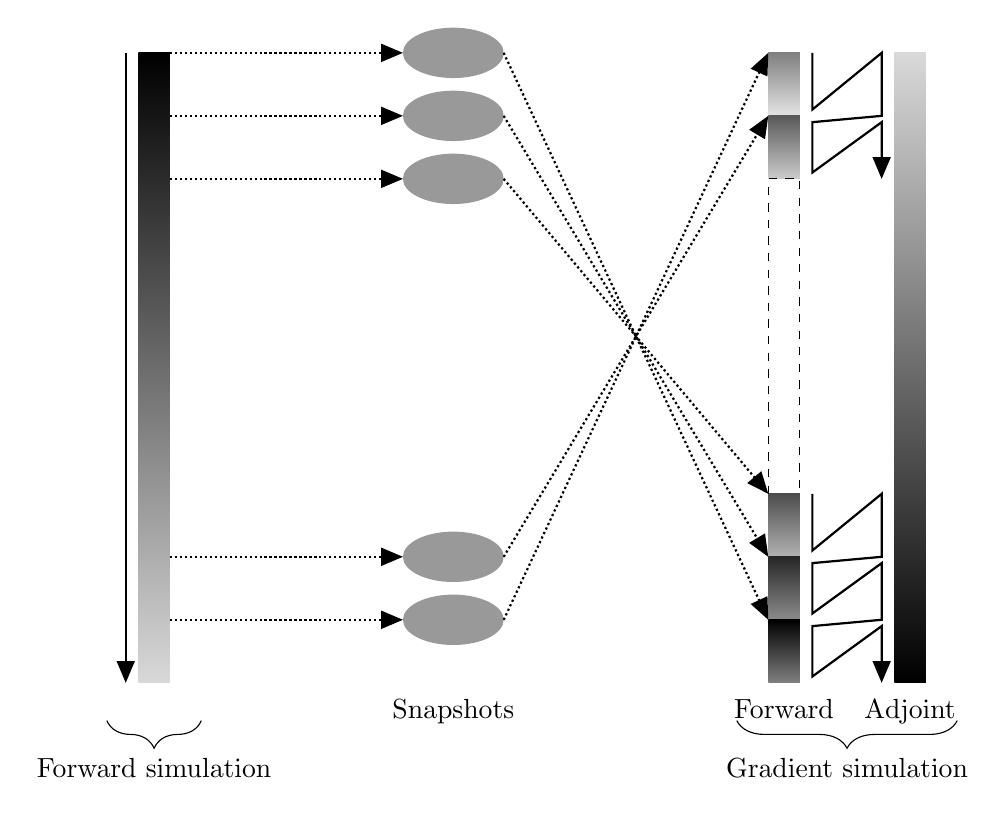
\begin{tikzpicture}[scale=0.8]

% forward bar
\shade [top color = black, bottom color = black!15!white] (0,0) rectangle +(0.5,10);

% adjoint - forward bar
\shade [top color = black!50!white, bottom color = black!10!white] ((10,9) rectangle +(0.5,1);
\shade [top color = black!65!white, bottom color = black!20!white] ((10,8) rectangle +(0.5,1);
%\shade [top color = black, bottom color = black!15!white] ((10,7) rectangle +(0.5,1);
\draw [dashed] (10,3) rectangle +(0.5,5);
\shade [top color = black!70!white, bottom color = black!30!white] ((10,2) rectangle +(0.5,1);
\shade [top color = black!85!white, bottom color = black!45!white] ((10,1) rectangle +(0.5,1);
\shade [top color = black, bottom color = black!50!white] ((10,0) rectangle +(0.5,1);

% adjoint - adjoint bar
\shade [top color = black!15!white, bottom color = black] (12,0) rectangle +(0.5,10);

% snapshots
 \fill [color = black!40!white] (5,10) circle [x radius=8mm, y radius=4mm];
 \fill [color = black!40!white] (5,9) circle [x radius=8mm, y radius=4mm];
 \fill [color = black!40!white] (5,8) circle [x radius=8mm, y radius=4mm];
 %...
 \fill [color = black!40!white] (5,2) circle [x radius=8mm, y radius=4mm];
  \fill [color = black!40!white] (5,1) circle [x radius=8mm, y radius=4mm];

% forward to snapshots
 \draw [->, thick, densely dotted, > = triangle 45] (0.5,10) --(4.2,10);
 \draw [->, thick, densely dotted, > = triangle 45] (0.5,9) --(4.2,9);
 \draw [->, thick, densely dotted, > = triangle 45] (0.5,8) --(4.2,8);
%...
 \draw [->, thick, densely dotted, > = triangle 45] (0.5,2) --(4.2,2);
 \draw [->, thick, densely dotted, > = triangle 45] (0.5,1) --(4.2,1);

% snapshots to adjoint - forward
 \draw [->, thick, densely dotted, > = triangle 45] (5.8,1) --(10,10);
 \draw [->, thick, densely dotted, > = triangle 45] (5.8,2) --(10,9);
%...
 \draw [->, thick, densely dotted, > = triangle 45] (5.8,8) --(10,3);
 \draw [->, thick, densely dotted, > = triangle 45] (5.8,9) --(10,2);
 \draw [->, thick, densely dotted, > = triangle 45] (5.8,10) --(10,1);

% forward timeline
\draw [->, thick, > = triangle 45] (-0.2,10) -- (-0.2,0);
% adjoint timeline
 \draw [->, thick, > = triangle 45] (10.7,10) -- (10.7,9.1) -- (11.8,10) --(11.8, 9) -- (10.7, 8.9) 
 						-- (10.7,8.1) -- (11.8, 8.9) -- (11.8, 8);
 \draw [->, thick, > = triangle 45] (10.7,3) -- (10.7,2.1) -- (11.8,3) --(11.8, 2) -- (10.7, 1.9)
 						-- (10.7,1.1) -- (11.8, 1.9) -- (11.8, 1) -- (10.7, 0.9) -- (10.7, 0.1)
						-- (11.8, 0.9) -- (11.8, 0);

% Legend
\node [align=center,below] at (5,-0.1) {Snapshots};
\node [align=center,below] at (10.25,-0.1) {Forward};
\node [align=center,below] at (12.25,-0.1) {Adjoint};

\draw [decorate,decoration={brace,amplitude=10,mirror},yshift=0]
(9.5,-0.6) -- (13,-0.6) node [black,midway,xshift=0, yshift=-17] {Gradient simulation};
\draw [decorate,decoration={brace,amplitude=10,mirror},yshift=0]
(-0.5,-0.6) -- (1,-0.6) node [black,midway,xshift=0, yshift=-17] {Forward simulation};
\end{tikzpicture}


%\end{document}  

    \caption[I/O pattern with full attenuation]
    {I/O pattern with full attenuation. The forward simulation (left bar) produces
snapshots at regular intervals. During the kernel simulation (right bars) these
snapshots are read in reverse order to piece-wise reconstruct the forward
wavefield for a number of time steps. The interaction of this reconstructed
wavefield with the adjoint wavefield yields to the so-called event kernels,
the sum of which is the misfit gradient. Solid arrows depict computation order, dashed arrows represent I/O.
Bars shade from black to light gray jointly with forward time.}
    \label{fig:undo_att_scheme}
  \end{center}
\end{figure}



\subsection{Parallel file formats and I/O libraries for scientific computing}
\label{subsection:ADIOS}

Although I/O libraries and file systems must be considered together to improve
I/O techniques, only I/O libraries are exposed to the scientific programmer. In
what follows, we try to focus our efforts on a more library-oriented approach.

The POSIX standard defines an I/O interface designed for sequential processing.
Its single \emph{stream of bytes} approach is well known to poorly scale on
distributed memory machines. Extensive studies tried to extend this
standard~\cite{Vilayannur2008}, most of the time in combination with research on
parallel file systems.%~\cite{Carns2000}.

When considering parallel software, developer choices have a great impact on how
I/O calls perform. There are two simple ways to use the POSIX I/O interface in
such parallel software:
\begin{itemize}
\item The most straightforward method is having separate files for each task.
Eventually, subsequent processing can be applied on subsets of files to gather data.
For a large number of tasks, this approach leads to a large number of files,
potentially causing contention on the file system metadata servers.
\item Each process sends its data to a set of master MPI tasks in charge of
writing data to disk. Conversely, data can be read from disk by a subset of MPI
tasks and then distributed among all MPI tasks. This approach has a few
drawbacks. In particular, nodes running master tasks might run out of memory if
the number of scattered/gathered data is high. Moreover, network traffic is
likely to reach high levels, slowing down the execution.
\end{itemize}

Over the past decades, a number of techniques has been developed and
incorporated into libraries  to ease writing ---sometimes large amounts of data---
to disk.
%\subsection{Parallel I/Os}
Our goal is not to provide a full description of parallel I/O techniques and
libraries evolution. Fur this purpose, the reader may consult Schikuta and
Vanek~\cite{Schikuta2001} or Liu et al.~\cite{Liu2013}. However, we do believe
that understanding where the need for simple and generic APIs comes from helps
determine a solution satisfying our needs. In what follows, we consider
distributed memory systems and software programmed using MPI, to date the most
common paradigm to address large scientific simulations on modern HPC systems.

The first version of MPI did not define a dedicated I/O API. Parallel I/O
libraries were often developed to match particular architectural or applicative
requirements. For instance, ChemIo~\cite{Nieplocha1998} was developed as an
interface for chemistry applications and SOLAR~\cite{Toledo1996} to accelerate
writing dense out-of-core matrices. Thakur et al.\ developed ADIO
(Abstract-Device interface for parallel I/O)~\cite{Thakur1996}
to fill the gap between various parallel filesystems and parallel I/O libraries.
This work ultimately lead to ROMIO~\cite{Thakur1999}, one of the most popular
MPI-IO libraries that was later integrated as a component into the well-known
MPICH2 library. While MPI-2 introduced support for parallel I/O with the MPI-I/O
approach, using it in large scientific code is not always straightforward. As a
matter of fact, it is a low level API writing raw data to files and demands a
concerted effort from the scientific programmer.

%\subsubsection{Metadata file formats}

Scientific software can benefit from libraries wrapping complexity into a higher
level function set. Hence, libraries accommodating metadata were designed to
ease further exploitation of produced data. Two of the most popular parallel I-O
libraries embedding metadata are netCDF~\cite{Li2003} and
HDF5~\cite{Howison2010}. Both of them provide a parallel interface. While netCDF
is principally oriented toward the storage of arrays ---the most common
scientific data structure--- HDF5 is more versatile and based on user-defined data
structures. The distinction between these two libraries became blurrier as
netCDF, starting from version 4, is implemented through HDF5. Metadata allow
further analysis on potentially large datasets in providing the necessary
information to fetch values of interest. A significant number of well
established tools are based on this format, showing their durability.

%Although these libraries help designing better data file structures and ease the life of the  programmer, their primary intent was not to scale on large numbers of processing nodes, and a lot of optimization is required.

%\subsubsection{The ADIOS library}

An alternative is the ADIOS library~\cite{Liu2013}
%\cite{Lofstead2008, Liu2013}
released by ORNL. Compared to netCDF and HDF5, it works on simpler data
structures since its main focus is parallel performance. Besides metadata
availability similar to the other formats previously mentioned, it also lets
users change the transport method to target the most efficient I/O method for a
particular system or platform. A set of optimizations is embedded in so called
\emph{transport methods}. I/O experts have the option to develop new transport
methods while scientific developers have to pick one matching the platform,
their software and their simulation case. In particular, transport methods
describe the file pattern, that is to say, if a number of MPI tasks write data
to the same number of files, to a smaller number of files or to a single file.
The underlying optimizations contain methods such as aggregation, buffering, and
chunking, and are transparent to the user.

Two APIs are available, one POSIX-like API with a reduced number of functions
and one XML API which is not as flexible as the regular API but allows one to
keep I/O separated from the main program.

From a user perspective, reading data is very similar to writing them. It must
be noted that it is possible to read and write data form a \emph{staging} memory
area, thus limiting disk access when produced data are consumed right away.

Although the ADIOS library needs to be improved by providing optimizations tuned
for a larger number of file systems (GPFS for instance), its architecture allows
domain scientists to focus on the actual problem.

Liu et al.~\cite{Liu2013} demonstrated excellent improvements in terms of I/O
speed. For instance, both S3D, software simulating reactive turbulent flows, and
PMCL3D, a finite-difference based software package simulating wave propagation,
show a 10 fold improvement when switching from MPI-IO to ADIOS. They managed to
write at a 30\,GB/s rate when using 96K MPI tasks for S3D and 30K MPI tasks for
PMCL3D.

\subsection{Integrating parallel I/O in adjoint-based seismic workflows}

%\subsubsection{Constraints}

%The previous section described two different types of data. The different purposes of these data imply different constraints.

%The main bottlenecks in the adjoint tomography workflow stem from the number of files to be read and written, which reduces performance significantly and creates problems on filesystems due to heavy I/O traffic. Classical seismic data formats, which describe each seismic trace as a single file, exacerbate this problem. Moreover, since we are considering large seismic simulations on the latest supercomputers, we have a particular concern about parallel performance.

%It is apparent that the classical data formats neither fulfill the computational requirements on HPC systems nor the provenance of computations and analysis for reproducibility of experiments. Furthermore, the lack of a common and flexible data format, both seismic and computational, has been a major problem in the seismological community, restricting the exchange of data and Earth models, and thus collaborative science.

%Geophysical variables might be shared across the scientific community for further reference or study. Thus, such data must keep track of their full history for reproducibility purpose. Further extraction and processing imposed that data are stored in a flexible and convenient format.


%\subsubsection{Optimizing computational data}

Computational data, in general, do not require complex metadata since they are
well structured within numerical solvers. In legacy
\texttt{SPECFEM3D\_GLOBE}, the way computational data were written to disk was
not problematic on local clusters for smaller size scientific problems (e.g.,
regional- or continental-scale wave propagation, small seismic data sets, etc.).
However, to run simulations more efficiently on HPC systems for more challenging
problems, such as global adjoint tomography or increased resolution regional-
and exploration-scale tomography, we needed to revise the way the solver handles
computational data. In the previous version of the \texttt{SPECFEM3D} packages,
for each variable or set of closely related variables, a file was created for
each MPI process. The number of files, for a single seismic event, was
proportional to the number of MPI processes~$P$.  For a full iteration of the workflow
the number of files was $\mathcal{O}(P.N_{s})$. Accessing
these files during large-scale simulations did not only have an impact on
performance, but also on the filesystem due to heavy I/O traffic. This is because of
the difficulty for the file system metadata server to handle all requests to
create the whole set of files. The new implementation uses ADIOS to limit the
number of files accessed during reading and writing of computational data,
independent of the number of processes, that is $\mathcal{O}(N_{s})$. Since
writing a simple file is also a potential bottleneck due to lock contention, we
are sometimes asked to change the transport method to output a limited number of
files. This is mostly invisible to the code user as these files are output as
subfiles that are part of a single file. As an additional benefit, using ADIOS,
HDF5 or netCDF let us define readers for popular visualization tools, such
as Paraview and VisIt.

Tests have been run to assess the I/O speed to write models in
\texttt{SPECFEM3D\_GLOBE} on the Titan supercomputer. The test case has been
chosen to match the number of processes and to result in the same amount of I/O
as the complete simulation for our 253 earthquake database. This results in more
than 6~millions ($6 \times 1007^2$) spectral elements on the Earth's surface,
processed through $24,576$ MPI tasks. ADIOS experts at ORNL indicated that the
preferred way to get I/O performance is to use the \texttt{MPI\_AGGREGATE}
transport method. This method is carefully tuned for large runs on Lustre
filesystems. Suitable parameters for this transport method were given by ORNL
ADIOS experts in order to match both OLCF Spider file system characteristics and
the test case parameters. A single ADIOS writer process was associated with 256
Object Server Targets (OST), 32 MPI tasks running on 2 Titan nodes. The test was
later reproduced on the new OLCF Atlas file system. Results in
Table~\ref{table:adios_perfs} show that switching from Spider to Atlas brings a
significant improvement in terms of I/O bandwidth. Moreover, in this case, the
peak bandwidth on the Spider filesystem is 16.9 GB/s, while on the Atlas
filesystem the peak bandwidth is 51.5 GB/s. This is likely to be beneficial for
our research, especially when the spatial resolution is increased, yielding
large data volumes on a high number of nodes.
%However, for tomographic iterations with limited resolution, the performance level is expected to be lower.
%The first reason is that each simulation is independent and output relatively small files.
%The second reason is that ADIOS most efficient transport method (\texttt{MPI\_AGGREGATE}) do not support append mode.
%Different regions of the globe are computed separately and thus outputted at a different time. As visualization require to gather these different regions in a single file, appending successive regions is mandatory. This limitation is likely to be lifted in future ADIOS versions.


\begin{table}%1
%\noautomaticrules
  \caption[Benchmarks of I/O Bandwidth for ADIOS]
  {\small{Bandwidth for \texttt{SPECFEM3D\_GLOBE} output using the ADIOS
    \texttt{MPI\_AGGREGATE} transport method for mesh using 24,576 MPI tasks.
    Results are presented both for the old (Spider) and new (Atlas) OLCF
    filesystems. Numbers for different regions outline that large files benefit the
    most from use of the ADIOS library.}}
\begin{tabular}{@{}lccc@{}}
\tch{Mesh Region}    &\tch{Ouput Size (GB)} &\tch{Spider (GB/s)} &\tch{Atlas (GB/s)}\\[-2pt]
\midrule
Crust-Mantle     & $2, 548$             & $14.3$             & $40.6$               \\
Outer Core        & $317$                & $7.4$               & $8.47$               \\
Inner Core        & $177$                 & $4.8$              & $7.6$              \\
\end{tabular}
\label{table:adios_perfs}
\end{table}

\section{A Modern Approach to Seismic Data: Efficiency and Reproducibility}
\label{sec:asdf}
%\red{Wenjie}

Seismology is a science driven by observing, modeling, and
understanding data. In recent years, large volumes of high-quality seismic data
are becoming more and more easily accessible through the dramatic growth of
seismic networks. Together with the development of modern compute platforms,
both large-scale seismic simulations and data processing can be done
very efficiently. However, the  seismological community is not yet ready to
embrace the era of big data. Most seismic data formats and processing
tools were developed more than a decade ago and are becoming obsolete in many
aspects. In this chapter, we present our thoughts and efforts in bringing
modernity into the realm.

%\subsection{Introduction}

The very basic unit of seismic data is the seismogram, which is a time series of
ground motion recorded by a seismometer during an earthquake. Most seismometers on
land are able to record 3-component data: one vertical component, and two
horizontal components perpendicular to each other(usually east and north) while
seismometers in the ocean vary, some are equipped with a water pressure sensor and
others record 3-component displacement of the seabed (an Ocean Bottom
Seismometers). Seismometers are recording 7/24 and data are archived at data
centers. The data we are primarily interested in are 3-hour time windows after
an earthquake, during which time seismic waves propagate inside the
earth and gradually damp out.

\subsection{Legacy}

Most earthquake seismologists are familiar with Seismic Analysis Code (SAC, see
\cite{HelffrichWookeyBastow201311}), a general-purpose program designed for the
study of time series. It provides basic analysis capabilities, including general
arithmetic operations, Fourier transforms, filtering, signal stacking,
interpolation and etc., which fit the general requirements of researchers.

Alongside the software package, SAC also defines a data format, which has been
widely used by seismologists over the last few decades. In the SAC data format,
each waveform (time series) is stored as a separate data file, containing a
fixed length header section to store metadata, including time and location
information), followed by the data section (the actual time series). Thus, for
one earthquakes recorded by 2,000 seismometers, one would expect 6,000 independent
SAC files. The main reason SAC is popular within the seismological
community is its ease of use and its interactive command line tools. Even though
functionality is limited, SAC covers the most frequent needs of
seismologists. For example, visualizing seismograms is very easy in SAC and is
frequently used to check the effect of operations applied to data.
% What is more, considering the resource, both on data availability and
% computation power, are quite limited, even though the definition SAC data format
% is simple, it is sufficient for users at that time.

However, things are evolving quickly as more and more seismometers are
installed. For a single network, the number of seismometers can go easily beyond
$1,000$, leading to sizable datasets. Thus, SAC and its associated format is
no longer a good choice for the following reasons.
\begin{itemize}
    \item It has limited non-programmable functionalities.
      SAC tools have to be invoked by system calls (shell scripts) and the lack of APIs for programming
      languages, such as C and Fortran, makes it difficult to customize workflows.
    \item The SAC data format only stores one waveform per file.
      Given 5,000 earthquakes and 2,000 stations for each earthquake,
      $3*10^7$ SAC files have to be generated and stored. Reading or
      writing such a large number of files is highly inefficient,
    \item The header in the SAC data format is very limited, with only
      a fixed number of pre-defined slots to store metadata. However, a modern
       data format should be flexible enough for users to define metadata relevant to
       the problem they are solving. Imposing pre-defined offsets in bytes
       to access information is a recipe for disaster.
    \item Station information, which contains instrument response information,
    is stored in separate files. This approach increases the number of files to deal
    with and the possibility of making errors.
    Having the ability to store station information along with the waveform data
    greatly reduce the chances of mistakes.
\end{itemize}

\subsection{The Adaptable Seismic Data Format}

We looked for existing solutions lacking the drawbacks listed in the previous
paragraph.
Because introducing a new data format should ideally be avoided,
the seismological community has been postponing the
definition of more modern approaches.
We believe that the advantage of a new data format are significant
enough to quickly outweigh the initial difficulties of switching to a new
format. We identify five key issues that the new data format must resolve.
\begin{itemize}
  \item \textbf{Robustness and stability}: The data format should be stable enough
  to be used on large datasets while ensuring data integrity and the correctness of scientific results.
  \item \textbf{Efficiency}: The data format should be exploitable by efficient, parallel tools.
  \item \textbf{Data Organization}: Different types of data (waveform, source \& station information,
    derived data types) should be grouped at certain levels to perform a variety of tasks. The data
   should be self-describing so no extra effort is needed to understand the data.
  \item \textbf{Reproducibility}: A critical aspect of science is the ability to reproduce
    results. A modern data format should facilitate and encourage this.
  \item \textbf{Mining and Visualization of data}: Data could be queried and visualized anytime
    in an easy manner.
\end{itemize}

The Adaptable Seismic Data  Format (ASDF)~\cite{krischer2016adaptable} was introduced to
solve these issues.
Using HDF5 at its most basic level, it organizes its data in a hierarchical
structure inside a container ---in a simplified manner a container can be
pictured as a file system within a file.

HDF5 was chosen as the underlying data format for a variety of reasons.
First, HDF5 has been used in a wide variety of scientific projects and
has a rich and active ecosystem of libraries and tools. It has a number of
built-in data compression algorithms and data corruption tests in the form of
check summing.
Second, it also fulfills our hard requirement of being capable of parallel I/O
with MPI~\cite{MPI, Howison2010}.
Besides, there is no need to worry about the endianness of data, which
historically has been a big issue in seismology.

An ASDF file is roughly arranged in four sections, as follows.
\begin{enumerate}
    \item Details about seismic events of any kind (earthquakes, mine blasts,
        rock falls, etc.) are stored in a QuakeML document.
    \item Seismic waveforms are grouped seismic station
        along with meta information describing the station properties
        (a StationXML document).
    \item Arbitrary data that cannot be understood as a seismic waveform are
        stored in the auxiliary data section.
    \item Data history (provenance) is kept as a number of SEIS-PROV
     documents (an extension to W3C PROV).
\end{enumerate}

Existing and established data formats and conventions are utilized wherever
possible. This keeps large parts of ASDF conceptually simple, and delegates
pieces of the development burden to existing efforts. The ASDF structure is
summarized in Figure~\ref{fig:asdf_container}. With such a layout, every
seismograms of a given earthquake can be naturally grouped into one ASDF file.
Also, event information and station information are incorporated so no extra
files have to be retrieved during processing.

Reproducibility is frequently discussed and widely recognized as a critical
requirement of scientific results. In practice, it is a cumbersome goal to
achieve and is frequently ignored. Provenance is the process of keeping track of
and storing all constituents of information that were used to arrive at a
certain result or at a particular piece of data. The main goal of storing
provenance data directly in ASDF is that scientists looking at data described by it should be able to tell what
steps were taken to generate that particular piece of data. Each piece of
waveform and auxiliary data within ASDF can optionally store provenance
information in the form of a W3C PROV or SEIS-PROV document. Thus, such a file
can be safely archived and exchanged with others, and information that led to a
certain piece of it is readily available.

More details about ASDF may be found in \cite{krischer2016adaptable}.

\begin{figure}[htb!]
  \centering
  \includegraphics[width=0.8\textwidth]{ch-workflow/figures/ASDF_container_bw}
  \caption{Layout of the Adaptable Seismic Data Format, including earthquake
  event information, waveforms and station meta information, auxiliary data and
  provenance. In such layout, different types of data are grouped into
  one file and ready for later retrieval.}
  \label{fig:asdf_container}
\end{figure}

\subsection{Data Processing}

Global adjoint tomography is ideal for the ASDF data format.
First, the data volumes involved are massive, easily containing millions of
seismograms. Second, it necessitates sophisticated processing to turn raw data
into meaningful results. Here, we present a typical data processing workflow
occurring in full seismic waveform inversions with adjoint techniques
\cite{Tromp2005, Fichtner2006, Tape2010, zhu2012structure}.
The general idea also
translates to other types of tomography (see \cite{Liu2012} for a recent
review).

To enable a physically meaningful comparison between observed and synthetic
waveforms, time series need to be converted to the same units and filtered in a
way that ensures a comparable spectral content. This includes standard
processing steps like detrending, tapering, filtering, interpolating,
deconvolving the instrument response, and others. Subsequently, time windows in
which observed and simulated waveforms are sufficiently similar are selected and adjoint sources
are constructed from the data within these windows, see
Figure~\ref{fig:adjoint_workflow} for a graphical overview.

\begin{figure}[htb!]
  \centering
  \includegraphics[width=0.8\textwidth]{ch-workflow/figures/adjoint_workflow_bw}
  \caption{Workflow of seismic data processing using ASDF. First, time
  series analysis is applied to raw observed and synthetic data to ensure a
  comparable spectral content at a later stage. Then, time windows are selected
  for pairs of processed observed and synthetic data, inside which
  measurement are made. Finally, adjoint sources are generated as the
  final pre-processing output. ASDF speeds up these tasks by using parallel processing (MPI).
  For each step, processing information is added to the provenance.}
  \label{fig:adjoint_workflow}
\end{figure}

The following is an account of our experiences and compares a legacy workflow
to one utilizing the ASDF format, demonstrating the latter's clear advantages.
Existing processing tools oftentimes work on pairs of SAC files, observed and
synthetic seismic data for the same component and station, and loop over all
seismic records associated with any given earthquake.
Given the large number of seismic receivers and earthquakes, the frequent read
and write operations on a very large number of single files create severe I/O
bottlenecks on modern compute platforms.
The implementation centered around ASDF shows superior scalability for
applications on high-performance computers: observed and synthetic seismograms
of a single event are stored in only two ASDF files, resulting in a
significantly reduced I/O load.  What is more, it is beneficial to keep meta
information in the same file. For example, one does not need to reach out for
separate files that keep track of the stations' instrument information or files
containing earthquake information, which greatly reduces the complexity of
operations and the possibility of making mistakes. Last but not least,
provenance information is kept to increase reproducibility and for future
reference.

Other than the data format itself, the data processing workflow benefits from the extensive
APIs provided by ASDF. ASDF is supported in the \texttt{SPECFEM3D\_GLOBE}
package \cite{KoTr02a}. Synthetic ASDF files are
directly generated, meaning synthetic data can seamlessly be fed as an input
into the workflow. To maximize performance, we rewrote our existing processing
tools. A big drawback in the old versions was that codes were written in
different languages and unable to communicate with each other easily. For
example, the SAC package was used for
signal processing and the Fortran based FLEXWIN program \cite{maggi2009automated} for
window selection.
In the new version we treat tasks as individual components in a single cohesive
workflow. Relying on the seismic analysis package ObsPy \cite{obspy2010}, we
re-developed all workflow components in Python. Therefore, all components
integrate with each other and stream data from one unit to the next. I/O only
happens at the very beginning, when we read the seismogram into memory, and at
the very end, when we write out the adjoint sources. All in all these changes
empower us to increase the scale of our inversions ---in terms of frequency
content, number of earthquakes, and number of stations--- and fully exploit
modern computational platforms.


\section{Bringing the Pieces Together: Workflow Management}
\label{sec:workflow_management}
%\red{Matthieu}

%\subsection{Intro: Why do we need workflow management plan?}

The importance of a performant solver to simulate forward and adjoint wavefields
is well understood and accepted. In our case, sustained efforts are being made
to adapt and tune \texttt{SPECFEM3D\_GLOBE} to newer architectures.
One of the most significant benefits of this work is the ability to
use GPU acceleration.

The ever increasing performance level of the wave simulation software goes along
with rapidly growing data volumes. This offers new opportunities for improving
our understanding of the physics and chemistry of Earth's interior, but also brings
new data management and workflow organization challenges.

Existing geoscience inversion workflows were designed for smaller scientific
problems and simpler computational environments and suffer from I/O
inefficiency, lack of fault tolerance, and inability to work in distributed
resource environments.
Workflow management challenges are by no mean limited to
earthquake seismology, let alone to global adjoint tomography.
In exploration seismology, streamers can contain sixty thousand hydrophones,
and the number of shots can reach fifty thousand, requiring petabytes of
storage.
Even then, a crying lack of scalable seismic inversion software (outside
of proprietary, closely-guarded oil industry codes) poses a continuing obstacle
to robust and routine inversions.
Given data volumes in the petabytes and compute time requirements in tens to
hundreds of millions of core-hours, new workflow management strategies are needed.

This section starts with a discussion of some of the most widely used scientific
workflow management system and solutions that have been brought in
order to manage seismic workflow. We then expose the requirements for large-scale
seismic inversions and the design of a solution. Finally, additional challenges
are outlined.

\subsection{Existing solutions}

When researching which workflow engine would be the most appropriate for
global adjoint tomography, the need to restrict the signification of the word
\emph{workflow} emerges. Indeed, workflow and workflow management have very
different meanings depending on the application domain. While there is some degree of
similarity between business and scientific workflows ~\cite{Ludascher2009}, we
will exclusively consider tools focusing on the latter.

Even then, the number of tools available to manage scientific workflows is large. What
follows discusses the main options and is by no means exhaustive. For more
in depth reviews, the reader should consult
~\cite{Yu2005, Hemert2008, Curcin2008}.

Focusing on usability by domain scientists, we also restrict ourselves to tools
providing a higher level of abstraction, and forbid ourselves to directly work
with powerful but complex tools such as HTCondor~\cite{condor-practice}.
%Distributed computing has also a long history. E,g, Globus, HTCondor.

From an user experience point of view, and forgetting about technical details,
two competing approaches are available. The first one relies on graphical user
interfaces (GUI). Examples include Kepler~\cite{Altintas2004},
Taverna~\cite{Wolstencroft2013}, and Triana~\cite{Taylor2007}.
The second approach involves scripting and is implemented by
a number of workflow management systems, such as Swift~\cite{Wilde2009},
Pegasus~\cite{Deelman201517}, or Radical-Ensemble~\cite{Turilli2016}.
Scripting is particularly well suited to scientists familiar with both HPC systems
and software development. It allows for fast prototyping and flexible definition
of workflows. As such, it provide users with powerful exploratory tools.

In the field of geophysics, fully managed workflows seem to be the exception
rather than the norm. Of course, proprietary software geared toward the oil
industry exists, but their closed nature forbids us to adapt and use them to
perform global adjoint tomography.
Most of the daily research and production computational work rely on a mixture
of hand-written scripts steering more computationally expensive software such as
solvers and data processing packages. Each scientist, or group of scientists, has
their own set of scripts embedding a fair amount of specific knowledge about the
system they are running on. Needless to say, such an approach is nonportable and error prone.
Attempts to provided a more streamlined way of running these hand-written 
scripts have been made. Starting from the ever increasing importance of
reproducible research~\cite{Fomel2007}, Fomel et al.\ developed
Madagascar~\cite{Fomel2013}, where dependencies between tasks are managed with
SCons, a software build tool similar in essence to GNU Make.

As science workflows, computer systems, and workflow engines grow more mature and
complex, inter-disciplinary collaboration is mandatory to bring seismic
simulation and processing to the next level.
One major exception to the lack of fully managed seismic workflows is
CyberShake~\cite{Graves2011}, which aims is to compute probabilistic seismic
hazard maps. CyberShake developers have been experimenting and using a number
of workflow managers to schedule computations on a wide range of HPC centers.
Among the workflow managers CyberShake has been run under the control of are
Condor, Globus, Pegasus~\cite{Callaghan2010}, and Radical-Pilot.

The Hadoop ecosystem, a popular paradigm to perform distributed computations, is
worth mentioning. It has been used in production environments for many years by
the industry and is gaining traction in scientific computing, especially to
solve data-driven problems. For many scientific problems relying on HPC systems,
involving large, multi-nodes simulations, it has so far remained an exotic
approach. The frontier tends to blur, thanks to approaches such as Yarn. A non
critical, but interesting feature for a suitable workflow engine is to be
able to address both Hadoop and HPC systems. This is for example the case for
some of Radical-Pilot~\cite{Luckow2015} most recent developments.

\subsection{Adjoint tomography workflow management}

As each problem and domain has widely different requirements, we fill focus
on ad-hoc solutions suited to large-scale seismic inversions on leadership-class
resources, such has the ones provided by the DOE computing centers.

The first requirement for large-scale seismic inversions is performance along
with efficiency. Indeed, the number of core-hours required to perform a global
inversion being in the hundreds of millions, a suitable workflow
management system needs to ensure that a minimum amount of compute cycles are
wasted. Large compute centers have requirements on the size of jobs that are
allowed to run; as they are primarily designed to accommodate computations that
would not fit any other place. While elementary computations of a seismic
inversion do not fulfill this condition, the large number of simulations involved
does. This means that in order to match the queueing requirements, smaller-scale
jobs have to be bundled in batches. Ideally, the workflow management
system should be in charge of such accounting matters. This is, for instance,
one of the features offered by the Pilot approach.

A second condition is the ability to execute in a relatively heterogeneous
environment. Here, the concept of heterogenous environment is understood
differently than for its more traditional grid computing definition. Each
elementary part of the workflow is run on an homogenous machine, while different
parts are not. For instance, for our current global inversions, Titan is used
to run simulations while Rhea, an Intel-based commodity cluster, is used to
process data. Appropriate resources are also used for visualizing data and
data transfer.

Another reason to run seismic inversion under a workflow management system is
reliability. On large systems, the mean time between
failures~\cite{Cappello01112009} is reduced compared to smaller-scale systems.
This is specially true for systems, such as the ones provided by DOE facilities,
that are on the edge of what is technically feasible. Job failures due to
hardware and software errors as well has corrupted data do happen. Hand-tracking
causes of such failures when dealing with large data sets and numerous simulations
is time consuming and error prone. The ability for a workflow to account for
this failures and eventually relaunch jobs is become even more critical as we
are the number of earthquake we assimilate data from raise.

It is equally important to keep the user in mind and to follow the science
problem logic. The typical user is a domain scientist with experience running
simulations on large-scale supercomputers. While the computer science details
must be hidden from such users, they are usually fluent in developing scripts,
allowing some level of technical details to be exposed to them.
For this scenario, scripting is particularly well adapted as it provides a
dynamic environment to define and iteratively improve workflows. This
flexibility is a very desirable feature for our global tomographic inversion, where
the numerical algorithmic strategy needs to be adapted according to the decrease
in the misfit function and the lessons learned performing previous iterations.
Domain logic is also better accommodated by a flexible ad-hoc approach. From
experience, concepts such as direct acyclic graphs (DAG) are, surprisingly
enough, difficult to convey to domain scientists.
It is important to note that the previous remarks are specific to large-scale
exploratory computations by power-users on leadership systems. A better approach
for the broader community might very well be such that it includes a graphical
interface and does not require any knowledge of the underlying system.

Additionally, a desirable feature is workflow portability. As newer distributed
paradigms, such has Hadoop, are gaining traction across the scientific community,
being able to run part of the workflow, most likely data processing, on such
infrastructures would undoubtedly benefit us.


% Scientific workflows, and in particular seismic tomography workflows are
% becoming increasingly complex. One of the reason for this, is the increasing
% amount of data to process.
% We would like to be able to add flexibility. Flexibility is needed to be able to
% easily change or improve the processing steps. Flexibility might be required to
% target a large number of computer infrastructures. For now we are targeting
% supercomputers that offer the ability to compute everything in a single place.
% This requires the domain scientists to have such a system to its disposition.
% Cloud computing can help to increase the avail- ability of scientific software
% for everyone. However, such resources might not sit at the same place. Hence the
% necessity to look at more distributed workflow management.


% \\
% Familiarity. Follows the problem logic. Can be expressed in a manner that is
% understandable to the usual computational domain scientist (that is not the
% regular domain scientist -- one that is at least familiar with large-scale
% systems and problems; and also has some comprehension of the difficulties
% encountered to run large problem sets).
% \\
% Technical requirements. MPI-aware: ability to launch large simulations on
% supercomputers. Allows for ad-hoc optimizations (e.g. in our case, to run
% simultaneous runs.)

% Two proof-of-concept applications have been identified as of primary interest
% for the development of an Ensemble approach. The first, Seisflows is an
% open-source research-grade framework used to quickly prototype and assess the
% numerical performances of inversion methods. It typically deals with a small to
% moderate amount of data and medium-sized computations (both for exploration and
% seismology problems) and runs an inversion from start to finish. The second is
% the adjoint tomography of the entire earth which requires tremendous amount of
% computational power to assimilate a large number of earthquakes at high
% resolution. The computational steps are similar to Seisflows, but due to the
% computational cost, a higher level of user interaction is required. In
% particular, visual checks of the gradient should be made possible after each
% iteration. Even though the computational focus of the two applications is
% different (one emphasizing full automation, the other striving for computational
% performance), a carefully designed Ensemble toolkit will enable the whole
% adjoint-based seismic inversion family of applications under a unified umbrella.
% In addition to facilitating truly large-scale inversions, our proposed scalable,
% flexible inversion toolkit stands to benefit a much larger inversion community
% working at small to medium scales. By being capable of interfacing with the
% popular, open source SPECFEM solvers and by leveraging the existing Seisflows
% user base, an ensemble toolkit will start as well-positioned workflow manager,
% which through functionality and ease of use, will attract additional inversion
% practitioners moving forward. Moreover, as discussed, new scientifically
% compelling anisotropic inversion capabilities will follow naturally, as well as
% new capabilities for assimilating data from thousands of earthquakes and
% performing simulations at higher frequencies – down to 1Hz.
% \\

% \\
% The goal is not to provide users with a completely effortless workflow. Indeed,
% a scientific workflow is exploratory and thus very different in nature than a
% business workflow. Its maturation follows the understanding of the science
% problem and as as matter of fact is iterative.

\subsection{Moving toward fully managed workflows}

From this panorama of existing workflow management systems and requirements, we
can see what a suitable solution for large-scale seismic inversion is.

%Need to separate the how from the what
Past experience on defining scripts ranging from simple bash scripts to
sophisticated modular python scripts taught us the need to separate the
application domain from the engine running the workflow.
This has several benefits, the most immediate being able to take advantages
of the most recent advances in the application domain and in workflow science.
Decoupling is also a good software engineering practice, as each part can be
implemented, tested, and maintained independently. For instance, the application
domain pieces might be used as standalone applications or plugged in different
workflow engines. Similarly, the workflow engine can evolve to exhibit common
patterns for a class of problems and thus be reused.
However, this does not mean that each side should not be designed with the other
one in mind. Indeed, complex inverse workflows impose significantly more complex
and sophisticated resource management and coordination requirements than simple
parameter sweeps in that they support varying degrees of coupling between the
ensemble members, such as global or partial synchronization. In addition, all
parts of the workflow must successfully complete to yield a meaningful scientific
result.

From the previous requirements, and after surveying a few workflow management
systems, it appears that two of them are particularly well suited to our needs:
Pegasus and Radical-Pilot.

The first step to be able to take advantages of such tools is to ensure the most
desired separation between the science software and the workflow management
system. Due to the number of steps involved in processing seismic data
(as explained in Section~\ref{sec:asdf}) and to create adjoint sources, we picked this
stage of the inversion workflow as the first sub-workflow to implement.

An important preparation has been to define clear interfaces for each of the
executables. That is, each executable must clearly define its inputs and outputs
without assumptions such as their relative location.
Different parts can then be assembled, either as a DAG (in the case of Pegasus),
or as an ad-hoc dependency description (in the case of Radical-Pilot).
We experimented with both, and consideration over the end-user experience
oriented our choice toward the latter.

To operate, workflow engines store information about job statuses along with
data useful to their internal machinery. Information of interest to the
scientist and to the science workflow, regardless of the engine, also need to be
tracked.
We have chosen to have information relevant to our pre-processing workflow
stored in an SQLite database. This database is regularly polled by the workflow
engine to dynamically create and launch jobs along with relevant parameters. Its
purpose is two-fold: to feed the workflow engine and to keep track of the
assimilated data. The process is described in
Figure~\ref{fig:workflow_management}.

\begin{figure}[htbp] %  figure placement: here, top, bottom, or page
   \centering
   \includegraphics[width=5in]{ch-workflow/figures/WorkflowManagement.pdf}
   \caption[Steering process of the workfow management system]
   {Steering process of the workflow management system. Two objects (DB
   manager and Job Manager) serve as an interface between the database and the
   workflow engine. The job manager requests data from the DB manager~(1), which
  polls an SQLite database~(2). Once the request is served~(3), executables,
   parameters, and inputs are formatted (4) to feed the workflow engine~(5). The
   workflow engine transparently launches the job and monitors its status, which is
   then returned~(6). The status is used to update the database~(7, 8) in order
   to keep track of the inversion status. This process is repeated~(9), until
   everything has been processed.}
   \label{fig:workflow_management}
\end{figure}

For now, the workflow engine is rudimentary and relies on Radical-SAGA to launch
jobs. Adapting it to a more complete solution, similar to Ensemble-MD, is
ongoing. Relying on Radical-Pilot, patterns common to seismic inversions would
be exhibited and released to the public.

\subsection{Additional challenges}

As we progress through the implementation and the understanding of automated
seismic inversion workflows, several challenges worth mentioning will need to
be taken care of.
Taking full advantage of large-scale resources requires tight software
integration. For instance, some next generation supercomputers will have burst
buffers allowing staging of data between computing steps. While this is a promise
of greater performance, this is problematic from a workflow management
perspective. Indeed, such techniques disrupt the control flow and defy the
purpose of a workflow engine. How to solve this is an open question.
A second challenge comes from the desire of scientists to visualize intermediate
data. This is motivated by the will to take informed decisions to steer the
inversion process in the best direction possible. This calls for a level of
interactivity that interfaces well with an automated approach.

It is equally important to start thinking from the beginning about the general
geophysicist population and how they can benefit from developments made
for large-scale inversions. We are confident that the pattern defining approach
of the Ensemble toolkits, along with the system-agnostic Radical-SAGA backend,
is a step toward dissemination.
% \\
% During the first tests, our work has been carried out on a local machine with a
% personal HTCondor installation. More advanced test have been performed on a
% virtual machine running Ubuntu. This virtual machine is spawned by Vagrant,
% using Chef recipes. In the longer term this will allow seamless deployment of
% the seismic inversion workflow on a variety of computational infrastructures.


\section{Software Practices}
\label{sec:software_practices}

The number and complexity of the software packages that we have developed, in order to be able
to perform exascale seismic inversions, have required us to adopt more rigorous
software practices.

Compared to professional software development teams, scientific software
developers face particular issues.
First, they are often a group of independent researchers that are in different
physical locations.
Second, there is often a large range in the level of programming
experience.
To address these issues, we implemented a simple
collaborative workflow based on modern software development techniques, such as
Agile
development and Continuous Integration/Continuous Development.

The two main goals of this workflow are to facilitate communication between
the developers, and to ensure that new software developments meet some agreed
upon quality criteria before being added to the common code base.
In practice, we have implemented this workflow using the tools provided by the
GitHub platform, and the automatic testing frameworks Buildbot, Jenkins and Travis CI.

%As illustrated in Figure \ref{fig:ReposBranches_all}, our collaborative
Our collaborative
software development practice
is organized around three Git repositories.
\begin{description}
\item[The central repository:] where the code is shared among developers, and
where users can download releases of the code.
\item[Forks of the central repository:] where each developer can post their
changes to
be tested by Buildbot, before being committed into the central
repository.
\item[Local clones:] where each developer builds his/her changes.
\end{description}
The first two repositories are hosted on the Computational Infrastructure for
Geodynamics (CIG) GitHub organization. The third repository is on the
developers desktop or laptop.

%\begin{figure}[tbh!]
%\centering
%\resizebox{5in}{!}{\input{ch-workflow/figures/ReposBranches_all.pdf_t}}
%\caption{There are three types of Git repositories: the central repository on
%  GitHub, the developer's fork on GitHub, and the developer's clone on their own
%  machine. The only way for developers to commit their changes to the central
%  repository is through a pull-request, which the code maintainers must accept.
%  Short tests are run before the maintainers accept the changes. Longer, more
%  extensive, tests are run on daily and weekly bases, as well as when new
%  developments are transferred from the \texttt{devel} to the \texttt{master}
%  branches of the central repository. \label{fig:ReposBranches_all}}
%\end{figure}

An essential part of our workflow is the differentiation between production and
development code: the production code is in a Git branch called
\texttt{master}, and the
development code is in a branch called \texttt{devel}.
The code in the \texttt{master} branch is intended for users that are only
interested in
running the code, while the \texttt{devel} branch is intended for code
developers. The changes to the code are first committed to the \texttt{devel}
branch.
Development code is transferred to the \texttt{master} branch only after
extensive
testing.

A fundamental rule of our workflow is that code changes can only be
committed to the \texttt{devel} branch of the central repository through a
pull-request. This provides us with two important features: first it allows us
to test the changes before they are committed to the central
repository, and, second, it sends an e-mail notification to the group of
developers. The notification to the developers is important because  it lets
them  review the changes before they are committed to the shared repository.

We have two distinct roles within our developer's community: \emph{code
maintainer}
and \emph{code developer}. The code maintainer role consists of accepting the
code changes proposed by the developers. The code maintainers have push/pull
(or read/write) permissions to the central repository, while the developers
only
have pull (or read only) permissions. In addition, code maintainers cannot
accept their
own source code changes.

Assuming that a developer already has a clone of the central repository on
his/her local machine, a typical workflow for committing new code developments
%to the central repository is as follows (see Figure \ref{fig:ReposBranches_all}).
to the central repository is as follows.
\begin{enumerate}
\item The developer pushes his/her changes to his/her fork on GitHub.
\item He/she opens a pull-request.
\item Opening a pull-request triggers automatic testing of the changes.
\item The maintainers and developers are notified of the results of the tests.
If the changes failed the tests, then the developer needs to fix the problems
and follow the steps 1 through 4, if they pass the test, go to step 5.
\item Before they can be committed in the central repository, the code needs to
be
reviewed by other developers.
\item The maintainers accept the changes and the new code is committed to the
  \texttt{devel} branch of the central repository.
\end{enumerate}

For this workflow to be successful, it is crucial to have a carefully designed
test suite. We use three types of tests for our codes.
\begin{description}
\item[Compilation tests:] they consist in looping through all the available
compiling options (e.g. OpenMP, MPI, CUDA) and using different compilers
(GCC and Intel compilers).
\item[Unit tests:] they tests individual functions by checking the output for
some
  predefined set of input parameters.
\item[Functional tests:] in our case, functional testing refers to the testing
of
  the a set of features of the code. Concretely, we run full examples for which
we
  compare the computed seismograms with some precomputed reference seismograms.
\end{description}

The compilation, unit, and some functional tests can be all done within 15~min
of opening the pull-request. These quick tests are the only ones that are done
before a pull-request is accepted. Other tests, that take longer to execute, are
run on daily and weekly bases. If these tests fail, then some changes need to be
reverted, but at least the changes are recent and there are few of them, so it is
easy to find what needs to to be fixed; we failed but we failed early.

In conclusion, our experience over the past three years has shown this
software development workflow to balance simplicity and effectiveness. Its
simplicity has made it easy to adopt for both experienced and new developers,
without hindering new developments. Its effectiveness at detecting problems
early has ensured the stability of our central repository.
In addition, by making the changes to the code more visible, this workflow
has improved the communication within our developer's community and enabled the
release of increasingly more sophisticated software.

\section{Conclusion}

%Problem: increasing volume of data to assimilate. increasing resolution.

We have outlined some of the difficulties arising in modern computational
seismology. They stem from the need to simultaneously handle large data sets and
increased Earth model resolution. This is even more true when performing large-scale
inversions at leadership supercomputer centers. Even though the data
volumes might not be comparable to what is commonly referred as ``big data'',
data and workflow management are creating performance and filesystem issues on
supercomputers.

In order to be able to pursue our scientific goals on the next-generation
supercomputers we have devised several strategies.
For heavy computational I/O we now rely on ADIOS. The developers of ADIOS have
either tight links with US computing centers or are part of them. We rely on the
improvements they bring to the so-called transport method
to continue getting a satisfying level of performance.
To accommodate the attenuation snapshots required for anelastic simulations,
several additional strategies might need to be
developed as the specificities of next-generation machine are unveiled. We can think
about overlapping I/O calls with computations, or using on-node non-volatile
memory (NVMe) as a burst-buffer.

Interestingly enough, the focus of seismic inversion is shifting from pure
computations to a more balanced approach, where data is a first-class citizen, seen
as equally important as computations. Using a modern file format, such as ASDF,
including comprehensive metadata not only helps increase computational
performance, but also ensures reproducibility, and in the long term brings a
standard to seismic and computational data which will ultimately increase
collaboration within the seismological community.

The shear number of data and simulations is becoming increasing difficult to
manage. Workflow management has been sparsely used within the
seismological community and, to the best of our knowledge, not in production-scale
inversions. This last sentence might be controversial, but, in our
opinion, to be considered as managed, a workflow must provide the user with
automation going beyond a simple dependency description.
Workflow management is an exciting challenge, particularly with the present
effort of infrastructure designers (both hardware and software) to bring
\emph{HPC} and \emph{Big Data} systems closers.

Many other challenges remain and keep arising during our journey to perform
global adjoint tomography problems on exascale systems. Some of the more
thrilling include exploring deep-learning methods to assimilate data in a more
sensible fashion, as well as newer visualization techniques allowing scientists
to discover features in global Earth models with unprecedented levels of detail.

\section*{Acknowledgement}

This research used resources of the Oak Ridge Leadership Computing Facility at Oak Ridge National Laboratory, which is supported by the Office of Science
of the U.S.\ Department of Energy under Contract No.~DE-AC05-00OR22725.
\\
Additional computational resources were provided by by the Princeton Institute for Computational
Science \& Engineering and the Princeton University Office of Information
Technology Research Computing department.


%\bibliography{biblio,workflow,litterature}

\chapter{Software Resources\label{ch:implementation}}
\label{ch:software_resource}

Most of our software is open-source, hosted on either github (\url{https://github.com/}) or bitbucket (\url{https://bitbucket.org/}).
The repositories that I am the major contributor to are listed below. URLs for
repositories and DOI information is also listed with the software.\\

\noindent \textbf{pytomo3d} -- Low-level APIs for processing Stream objects\\
\url{https://github.com/computational-seismology/pytomo3d}\\
DOI: 10.5281/zenodo.55346\\

\noindent \textbf{pypaw} -- High-level APIs for processing ASDF files\\
\url{https://github.com/computational-seismology/pypaw}\\
DOI: 10.5281/zenodo.55346\\

\noindent \textbf{spaceweight} -- Geographical weighting calculations\\
\url{https://github.com/wjlei1990/spaceweight}\\
DOI: 10.5281/zenodo.56123\\

\noindent \textbf{pycmt3d} -- Source inversion software\\
\url{https://github.com/wjlei1990/pycmt3d}\\
DOI: 10.5281/zenodo.56124\\

\noindent \textbf{simpy} -- Seismic workflow management tools\\
\url{https://bitbucket.org/mpbl/simpy/src/master/}\\
(Matthieu Lefebvre and I are the main contributors to the simpy software.
Currently we provide limited access to this repository.)\\

Software that I contribute to is listed below.\\

\noindent \textbf{pyadjoint} -- APIs for measurements and adjoint sources\\
\url{https://github.com/computational-seismology/pyadjoint}\\

\noindent \textbf{pyflex} -- APIs for window selection\\
\url{https://github.com/computational-seismology/pyflex}\\

\noindent \textbf{pyasdf} -- ASDF I/O APIs\\
\url{https://github.com/wjlei1990/pyasdf}\\

Both pyflex and pyasdf are local forks for upstream repositories,
with customization for global adjoint tomography.


% Make the bibliography single spaced
\singlespacing

% add the Bibliography to the Table of Contents
\cleardoublepage
\ifdefined\phantomsection
  \phantomsection  % makes hyperref recognize this section properly for pdf link
\else
\fi
\addcontentsline{toc}{chapter}{Bibliography}

% include your .bib file
\bibliographystyle{plain}
%\bibliography{ch-asdf/library}
\bibliography{ref}
%\bibliography{ch-GLADM25/ref, ch-asdf/library}
%\bibliography{ch-asdf/library, ch-GLADM25/ref}

\end{document}
